% Remove the oneside option below for double sided printing (e.g. for final (post-viva) submission)
\documentclass[a4paper,12pt,oneside,openright]{book}

% Preamble commands go here
\renewcommand{\labelenumi}{\theenumi}
\usepackage{customisations}
\usepackage{rotating}

%% Some of the below packages may be useful to thesis writers in Physics
%% Googling `latex <packagename>' will usually give you some documentation
% \usepackage[load-configurations=abbreviations]{siunitx} % siunitx typesets physical units in a consistent manner
\usepackage{booktabs} % booktabs provides professional formatting commands for tables
\usepackage{amsmath} % amsmath provides extra maths symbols

\usepackage{textcomp} % textcomp provides extra text symbols (like a degrees celsius symbol)
\usepackage[flushleft]{threeparttable}
% \usepackage{tikz} % tikz is a package for drawing diagrams and adding annotations to figures
% \usepackage{threeparttable} % threeparttable allows for adding notes to tables
% \usepackage{eps2pdf} % eps2pdf allows background transformation of eps files to pdfs so they
%						work seamlessly with pdflatex. If using this with the LaTeX editor Kile,
%						you need to add --shell-escape before '%source', in
%						Settings -> Configure Kile... -> Tools -> Build -> build_pdflatex

% End preamble

% REPLACE THESE with your thesis title, your name and the date of submission of the thesis
\title{Red Supergiant Stars within the Local Group}
\author{Lee. R. Patrick}
\date{March 2016} % of submission

\begin{document}


% Thesis front matter - title page, abstract, acknowledgements, declaration and table of contents
% See customisations.sty to modify the title page or declaration
\singlespacing
\maketitlepage
\frontmatter
\eighteenptleading
%%%%%%%%%%%%%%%%%%%%%%%%%%%%%%%%%%%%%%%%%%%%%%%%%%%%%%%%%%%%%%%%%%%%%%%%%%%%%%
% Re include for the final thing!

% \chapter{Abstract}

Red Supergiant (RSG) stars are the most luminous stars in the infrared sky.
Their intrinsic luminosities combined with the low dust extinction observed
in this regime makes these objects very attractive to study in the near-infrared (IR).
In addition, RSGs are necessarily young objects,
as, they are tracers of recent star formation in extra-galactic
systems.
As the next generation of telescopes will be optimised for study in the near-IR,
it is clear that, in the coming years, RSGs will play a prominent role in the way that astronomers probe the local Universe and out to larger distances with
space-based observations.
Therefore, it is vital to better our understanding of these objects now and develop the
tools that will allow us to take full advantage of the suite of instrumentation
that will become available in the near future.
This thesis aims to further the understanding of RSGs by focusing on quantitative studies of near-IR spectroscopic observations.

To this end, I develop an analysis technique that uses spectroscopic and photometric observations to estimate stellar parameters of RSGs.
The observations are compared with synthetic spectra extracted from stellar model atmospheres, where departures from local thermodynamic equilibrium have been calculated for the diagnostic spectral lines.
This technique is tested thoroughly on synthetic and real observations and is shown to reliably estimate stellar parameters in both regimes when compared with input parameters and previous studies respectively.


Using the analysis routines developed in Chapter~\ref{ch:janal}, in Chapter~\ref{ch:ngc2100} I measure the chemistry and kinematics of NGC\,2100, a young massive cluster (YMC) of stars in the Large Magellanic Cloud, using near-IR spectroscopic observations of 14 RSGs taken with the new $K$-band multi-object spectrograph (KMOS).
I estimate the average metallicity to be $-$0.43\,$\pm$\,0.10\,dex, which is in good agreement with previous studies.
I compare the observed location of the target RSGs on the Hertzsprung--Russell diagram with that of a Solar-like metallicity YMC and show that there appears to be no significant difference in the appearance of the RSGs in these two clusters.
By combining the individual RSG spectra, I create an integrated-light cluster spectrum and show that the stellar parameters estimated, using the same technique as for individual RSGs, are in good agreement with the average properties of the cluster.
In addition, I measure -- for the first time -- an upper limit of the dynamical mass of NGC\,2100 to be 15.2~$\times$~10$^4$\,M$_{\odot}$, which is consistent with the literature measurement of the photometric mass of the cluster.


In Chapter~\ref{ch:ngc6822}, I present observations of RSGs in NGC\,6822, a dwarf irregular with a turbulent history, observed with KMOS.
The data reduction process with KMOS is described in detail, in particular
where the reduction has been optimised for the data.
Stellar parameters are estimated using the technique presented in Chapter~\ref{ch:janal} and an average metallicity in NGC\,6822 of $-$0.55\,$\pm$\,0.13\,dex is found, consistent with previous measurements of young stars in this galaxy.
The spatial distribution of metallicity is estimated and weak evidence is found for a radial metallicity gradient, which will require follow-up observations.
In addition, I show that the metallicities of the young and old populations of NGC\,6822 are well explained using a simple closed-box chemical evolution model, an interesting result, as NGC\,6822 is expected to have undergone significant recent interactions.


In Chapter~\ref{ch:ngc55}, I present multi-epoch KMOS observations of 22 RSGs in the Sculptor Group galaxy NGC\,55.
Radial velocities are measured for the sample and are shown to be in good agreement with previous studies. Using the multi-epoch data, I find no evidence for radial velocity variables within the sample.
Stellar parameters are estimated for 10 targets and are shown to be in good agreement with previous estimates.

I conclude this thesis by summarising the main results and present a first-look calibration of the relationship between galaxy mass and metallicity using RSGs.
By comparing the RSG metallicity estimates to metallicities estimated from $\sim$50\,000 Sloan digital sky survey galaxies, I show that the absolute metallicities of the two samples disagree. A more quantitative analysis requires additional RSG observations.

In addition, using $\sim$80 RSGs, with stellar parameters estimated in a consistent way, I show that there appears to be no dependence of the temperature of RSGs upon metallicity.
This is in disagreement with current evolutionary models, which display a temperature change of $\sim$450\,K over the studied range in metallicity.

Finally, I outline potential areas for future work, focusing on follow-up studies that have been identified as a result of the work done in this thesis.

% \bibliography{../journals,../books}


\singlespacing
% Uncomment this line if you need to declare published work which forms part of the thesis
% \declarationpublications{\cite{Conway2000}}
% \makedeclaration

% \chapter{Acknowledgements}

To acknowledge the contribution of everyone who has helped me complete this thesis in the last three and a half years would, no doubt, contribute significantly to the page count of this thesis.
To keep this reasonably concise, I would like to first acknowledge all of the help I've received from the people who do not have a specific mention in this section.
All of the friends and work colleagues who have encouraged and spurred me on over the last few years: your contribution is not forgotten and is certainly appreciated.

I would like to thank my supervisor, Chris Evans, for providing excellent support from the outset and keeping me focused on the important tasks in hand, as well as his meticulous quality control, which have improved this thesis greatly.
Throughout the course of this thesis, I have had some fantastic opportunities to go observing and attend productive conferences, which is all thanks to Chris' drive and enthusiasm.
Chris has been a great supervisor and friend, always using his skills and knowledge to keep me optimistic and striving for the next result.

I would also like to thank all of my collaborators, in particular Ben Davies and Rolf-Peter Kudritzki, for their help and hard work, particularly at some strange times of the day (night, depending upon your time-zone).
In addition, I would like to thank my fellow students who have provided support on a huge range of different topics, which has saved me countless time and effort.

On a personal level, I would like to thank Melanie Woodward, who has not only, made this journey of a PhD with me, but also made it so much more enjoyable. Mel has helped me celebrate the highs and helped me get back on the horse during the lows.
However, Mel has not only contributed to this thesis on a personal level.
The quality of writing in this thesis (I'm not ashamed to say) is high.
I'm not ashamed to say that because it is down to the fact that Mel is an excellent editor and has spent hours studying and commenting on this thesis, improving the style, readability and flow greatly.


I would like to thank my fellow students for supporting me on a personal level.
The ``Golden Age'' of U4, which I was lucky enough to be a part of, along with Fergus Cullen and Sandy Rogers, will live long in my memory.


% \cleardoublepage
% \phantomsection
% \addcontentsline{toc}{chapter}{\contentsname}
% \setcounter{tocdepth}{2}
% \tableofcontents

% \cleardoublepage
% \phantomsection
% \addcontentsline{toc}{chapter}{\listfigurename}
% \listoffigures

% \cleardoublepage
% \phantomsection
% \addcontentsline{toc}{chapter}{\listtablename}
% \listoftables
%%%%%%%%%%%%%%%%%%%%%%%%%%%%%%%%%%%%%%%%%%%%%%%%%%%%%%%%%%%%%%%%%%%%%%%%%%%%%%
% John's hack for the MNRAS biblography
\setlength{\bibhang}{2.0em}
\setlength\labelwidth{0.0em}

% Bibtex stuff:
\newcommand{\aj}{AJ}            % Astronomical Journal
\newcommand{\araa}{ARA\&A}      % Annual Review of Astron and Astrophys
\newcommand{\apj}{ApJ}          % Astrophysical Journal
% \newcommand{\apjl}{ApJLett}     % Astrophysical Journal, Letters % just use ApJ
\newcommand{\apjl}{ApJ}     % Astrophysical Journal, Letters
% \newcommand{\apjlett}{ApJLett}      % Astrophysical Journal, Letters % just use ApJ
\newcommand{\apjlett}{ApJ}      % Astrophysical Journal, Letters
\newcommand{\apjs}{ApJS}        % Astrophysical Journal, Supplement
\newcommand{\apjsupp}{ApJS}     % Astrophysical Journal, Supplement
\newcommand{\ao}{Appl.~Opt.}        % Applied Optics
\newcommand{\apss}{Ap\&SS}      % Astrophysics and Space Science
\newcommand{\aap}{A\&A}         % Astronomy and Astrophysics
\newcommand{\astap}{A\&A}       % Astronomy and Astrophysics
\newcommand{\aapr}{A\&A~Rev.}       % Astronomy and Astrophysics Reviews
\newcommand{\aaps}{A\&AS}       % Astronomy and Astrophysics, Supplement
\newcommand{\azh}{AZh}          % Astronomicheskii Zhurnal
\newcommand{\baas}{BAAS}        % Bulletin of the AAS
\newcommand{\jrasc}{JRASC}      % Journal of the RAS of Canada
\newcommand{\memras}{MmRAS}     % Memoirs of the RAS
\newcommand{\mnras}{MNRAS}      % Monthly Notices of the RAS
\newcommand{\pra}{Phys.~Rev.~A}     % Physical Review A: General Physics
\newcommand{\prb}{Phys.~Rev.~B}     % Physical Review B: Solid State
\newcommand{\prc}{Phys.~Rev.~C}     % Physical Review C
\newcommand{\prd}{Phys.~Rev.~D}     % Physical Review D
\newcommand{\pre}{Phys.~Rev.~E}     % Physical Review E
\newcommand{\prl}{Phys.~Rev.~Lett.} % Physical Review Letters
\newcommand{\pasp}{PASP}        % Publications of the ASP
\newcommand{\pasj}{PASJ}        % Publications of the ASJ
\newcommand{\qjras}{QJRAS}      % Quarterly Journal of the RAS
\newcommand{\revmodphys}{Rev.\ Mod.\ Phys.} %Rev Mod Phys
\newcommand{\skytel}{S\&T}      % Sky and Telescope
\newcommand{\solphys}{Sol.~Phys.}   % Solar Physics
\newcommand{\sovast}{Soviet~Ast.}   % Soviet Astronomy
\newcommand{\ssr}{Space~Sci.~Rev.}  % Space Science Reviews
\newcommand{\zap}{ZAp}          % Zeitschrift fuer Astrophysik
\newcommand{\nat}{Nature}       % Nature
\newcommand{\nar}{New Astron. Rev}       % New Astronomy Reviews
\newcommand{\iaucirc}{IAU~Circ.}        % IAU Circulars
\newcommand{\aplett}{Astrophys.~Lett.}  % Astrophysics Letters
\newcommand{\apspr}{Astrophys.~Space~Phys.~Res.}% Astrophysics Space Physics Research
\newcommand{\fcp}{Fund.~Cosmic~Phys.}  % Fundamental Cosmic Physics
\newcommand{\gca}{Geochim.~Cosmochim.~Acta}   % Geochimica Cosmochimica Acta
\newcommand{\grl}{Geophys.~Res.~Lett.} % Geophysics Research Letters
\newcommand{\jcp}{J.~Chem.~Phys.}   % Journal of Chemical Physics
\newcommand{\jgr}{J.~Geophys.~Res.} % Journal of Geophysics Research
\newcommand{\nphysa}{Nucl.~Phys.~A}   % Nuclear Physics A
\newcommand{\physrep}{Phys.~Rep.}   % Physics Reports
\newcommand{\physscr}{Phys.~Scr}   % Physica Scripta
\newcommand{\planss}{Planet.~Space~Sci.}   % Planetary Space Science
\newcommand{\procspie}{Proc.~SPIE}   % Proceedings of the SPIE

%
\newcommand{\farcm}{\mbox{\ensuremath{.\mkern-4mu^\prime}}}%    % fractional arcminute symbol: 0.'0
\newcommand{\farcs}{\mbox{\ensuremath{.\!\!^{\prime\prime}}}}%  % fractional arcsecond symbol: 0.''0
\newcommand{\fdg}{\mbox{\ensuremath{.\!\!^\circ}}}%             % fractional degree symbol:     0.°0
\newcommand{\arcdeg}{\ensuremath{^{\circ}}}%                    % degree symbol:  °
\newcommand{\sun}{\ensuremath{\odot}}%                          % sun symbol
\newcommand{\Teff}{\ensuremath{T_{\mathrm{eff}}}}%              % T_eff
\newcommand{\logg}{\ensuremath{\log g}}%                        % log g
\newcommand{\bv}{\ensuremath{B\!-\!V}}%                         % B-V
\newcommand{\ub}{\ensuremath{U\!-\!B}}%                         % U-B
\newcommand{\vr}{\ensuremath{V\!-\!R}}%                         % V-R
\newcommand{\ur}{\ensuremath{U\!-\!R}}%                         % U-R
\newcommand\ion[2]{#1$\;${\scshape{#2}}}%                       % ion, i.e., CII = \ion{C}{ii}
% Other commands & definitions:
\newcommand{\mdot}{\ensuremath{\dot{M}}}
\newcommand{\msun}{\ensuremath{M_{\odot}}}
\newcommand{\vsini}{\ensuremath{v_{\rm R} \sin i}}
\newcommand{\vrot}{\ensuremath{v_{\rm R}}}
\def\5{\footnotesize V\normalsize}
\def\4{\footnotesize IV\normalsize}
\def\3{\footnotesize III\normalsize}
\def\2{\footnotesize II\normalsize}
\def\1{\footnotesize I\normalsize}
\def\lam{$\lambda$}
\def\kms{$\mbox{km s}^{-1}$}
\def\p{$\phantom{:}$}
\def\a{$\phantom{^\ast}$}
\def\v{$\phantom{^{l}}$}
\def\pp{$\phantom{-}$}
\def\o{$\phantom{0}$}
\def\vr{$v_{\rm r}$}

\renewcommand{\theenumi}{\roman{enumi}}
% Include main matter here
\mainmatter
\eighteenptleading
\chapter{Introduction}\label{ch:intro}

\section{Shaping the Universe with Massive Stars} % (fold)
\label{sec:massive_stars}
Understanding how stars form and evolve is fundamentally important to understanding the physical processes which govern the Universe.
As congregations of stars are built up they form heavily structured galaxies where the complex internal interactions between stars and gas as well as the underlying stellar population are vitally important to the chemical and dynamical evolution of the galaxy~\citep[e.g.][]{2014ARA&A..52..291C}.
Stars die to produce black holes where massive stars are good candidates for producing the recently observed gravitational wave signature~\citep{2016PhRvL.116f1102A,2016arXiv160204735L,2016arXiv160300511W} and fundamentally, stars are at the heart of almost every area of study in astrophysics: from active galactic nuclei to exoplanets, solar system bodies to high-redshift galaxies; an understanding of stars and stellar evolution is vital in understanding these phenomena.

Stars form with various different masses ranging from the hydrogen fusion limit of $\sim$0.08\,M$_{\odot}$~\citep{1997ApJ...491..856B,2000ARA&A..38..337C} to an uncertain upper mass limit in excess of $\sim$100\,M$_{\odot}$~\citep[e.g.][]{2005Natur.434..192F,2012MNRAS.422..794E,2014A&A...568L..13W} and up to $\sim$300\,M$_{\odot}$ in extreme cases~\citep{2010MNRAS.408..731C}.
Massive stars~\citep[defined here as stars with initial masses $>$8\,M$_{\odot}$ e.g.][and expanded upon in Section~\ref{sec:lives}]{2014ARA&A..52..487S} are probably the most important type of star with respect to how they shape their surrounding environments throughout their lives and distribute chemical elements in their deaths.
Massive stars drive the ionisation of their surrounding birth cloud and are good candidates for the reionisation of the Universe~\citep[e.g.][]{1997ApJ...483...21H,2005SSRv..116..625C,2006ARA&A..44..415F}.
During the short lifetime of a massive star (detailed in Section~\ref{sec:lives}) massive stars expel material from their outer layers in strong winds at various evolutionary stages throughout their lives.
These winds help to distribute nuclear processed material throughout their parent galaxies and pollute the interstellar medium (ISM) with heavy elements.

In any given star forming galaxy, the massive star population dominates the light output across a the full spectrum of light.
Ultraviolet and optical light is dominated by hot massive stars~\citep{1998ARA&A..36..189K,2012ARA&A..50..531K} with temperatures of up to 50\,000\,K~\citep[e.g.][]{2011A&A...530L..14B}.
Whereas infrared light is dominated by the cool (4000\,K) evolutionary products of these hot massive stars, i.e. red supergiant stars (RSGs), which can be as luminous as entire galaxies in the near infrared (near-IR).

Given that massive stars are extremely luminous, they can be used as probes of chemical abundance in external galaxies.
Indirectly, by ionising their surrounding birth cloud, massive stars are used to study galaxy populations at early epochs of the Universe~\citep{2004MNRAS.348L..59P}.
In the more local Universe, massive stars can be used to probe the structure and chemical evolution of galaxies in great detail~\citep{2007ApJ...659.1198E,2008ApJ...681..269K,2008MNRAS.386..826E,2010AN....331..459K,2011A&A...530A.108E,2012A&A...542A..79C}.

In this thesis I expand and develop the methods by which we can study massive stars (in particular RSGs) in extragalactic environments.
The study of RSGs in external galaxies in reality spans two key astrophysical topics: stellar evolution and galaxy evolution.
By using RSGs as abundance probes I have been able to map the spatial distribution of metals in external galaxies as well as gain insight into the underlying physics which is used within evolutionary and atmospheric models.

In the coming years, RSGs will play a more central role in the study of extragalactic systems owing to their extreme brightness coupled with the fact that their peak luminosity is in the near-IR as well as the intrinsic advantages with dust extinction at these wavelengths.
This is particularly poignant when considering that the next generation of ground- and space-based telescopes will be optimised for study in the near-IR.

% subsection massive_stars (end)

\section{The Lives of Massive Stars} % (fold)
\label{sec:lives}

Stellar evolution is critically dependent upon the initial mass of the star.
A 10\,M$_{\odot}$ star has a very different evolutionary path to that of a solar mass star.
Their formation, subsequent evolution and eventual fate all depend upon how much mass the star is able to accumulate during its formation.
Therefore, an understanding of how massive stars are able to gather their mass is crucial to the understanding of how these objects evolve and end their lives.
To this end, I provide an outline of the main process by which star formation occurs (focussing on massive stars) in Section~\ref{sub:birth}. Section~\ref{sub:life_cycle} describes the evolution of a massive star after the onset of hydrogen-burning in the core up until the final stage of evolution before the star ends its life.
This leads onto Section~\ref{sub:death} which reviews the eventual fate of massive stars.

\subsection{Birth} % (fold)
\label{sub:birth}

Massive stars, as with lower mass stars, begin their lives within giant molecular clouds (GMCs), which are regions consisting of large clumps of interstellar material which have become over-dense with respect to the surrounding interstellar medium.
These clouds are typically 10$^{4}$--10$^{7}$\,M$_{\odot}$, extend over 50--100\,pc and represent the densest parts of the interstellar medium~\citep{Fukui10}.
In a high-mass molecular cloud, high- and low-mass star formation takes place.
Studies suggest that as the mass of the cloud decreases, so does the mass of the largest stars~\citep{Fukui10,Weidner10}; however, recent studies suggest that this may not be a universal property~\citep[e.g.][]{Bressert12}.

Within GMCs, over-dense regions continue to grow and eventually fragment into smaller cores.
If these dense cores consist of a region where the local mass is greater than the associated Jeans mass for the region, the region is unstable to gravitational collapse.
As the region collapses into a protostellar core, the optical depth increases, which gives rise to a large increase in temperature~\citep{Zinnecker07}.
The collapse proceeds until the radiation pressure exerted by the core is able to resist the gravitational collapse.
The system is now in hydrostatic equilibrium and evolution proceeds though accretion.
The collapsed core accretes matter from a surrounding disk which has condensed around the protostar.
Meanwhile, the core of the protostar contracts and increases the temperature of the core towards hydrogen-burning temperatures.
A larger protostar can accrete a larger amount of additional material from its surroundings and in turn grows to become a more massive star.
In lower mass stars, accretion ceases before the star reaches the main sequence; however, a more massive star can perturb a larger amount of material and hence continues to accrete matter even after the hydrogen-burning phase has begun in its core.
The ignition of hydrogen classically ends the period of formation, as the star now has a central energy source which governs the evolution for the remainder of time spent on the main sequence.
However, massive stars have one more crucial role to play in the process of star formation.
Massive stars end their lives as supernovae, ejecting fusion products back into the environment from which they were born.
The surrounding gas is shocked and compressed by this mass ejection event which can be the catalyst needed to produce more star formation in these environments (triggered star formation).
% Jeans Mass is the maximum mass a cloud of gas can have before it becomes unstable to gravitational collapse
% Optical depth is a measure of how much light is not dispersed in the line of sight I=I_{0}e^{-\tau}

This is a very simplistic, qualitative overview of the formation of massive stars.
In reality the exact processes governing these main stages of formation are complicated by various factors, for example, the effect of turbulence has been completely neglected in this discussion but has a vital role in many phases of star formation~\citep{McKee07}.
The relative importance of each of the processes involved is not well understood.
As of yet, there is no universal theory of how star formation proceeds in massive stars.

There are several crucial differences between low- and high-mass star formation.\footnotemark~
\footnotetext{The opinion in the literature seems to suggest that low-mass star formation continues as normal up until around $\sim$20\,M$_{\odot}$~\citep{Zinnecker07, Crowther12}, above this, star formation must take into account various complicating factors (see text).}
Massive stars have larger temperatures and hence produce a large amount of ionising photons.
This means that the accretion disk and outer envelope surrounding the massive star is photoevaporated and dissociated through interactions with these high energy photons.
As alluded to previously, massive stars continue to accrete matter while on the hydrogen-burning main sequence~\citep{Zinnecker07}.
Whereas, lower mass stars ($<$0.2\,M$_{\odot}$) spend at least 10\,Myr evolving towards hydrogen fusion~\citep{Luhman12}.
A key difference in the star formation across a large mass range is the role of accretion.
In lower mass star formation, accretion does not form significant amounts of the final mass of the star~\citep{Bonnell08}, whereas in higher mass star formation, accretion is generally accepted as a key role in accumulating the mass of the star~\citep{Kraus10}.


Exactly how accretion acts is subject to much debate.
Accretion is likely to proceed via competitive accretion~\citep{Bonnell01}.
This is where a large fraction of the star is accreted from its surrounding material.
In this scenario, the amount of material available for accretion is limited only by the surrounding environment.
A star at the centre of the potential well of the surrounding gas cloud will be able to accrete more material than a star on the outskirts and hence will grow larger.
As the star grows larger, it is able to accrete more and more matter.
Eventually, neighbouring stars will be forced to compete for the surrounding gas, and in this scenario, the largest star (i.e. the star at the centre of the potential well) will be able to accrete a larger amount of material~\citep[for a useful economical analogy -- the rich get richer --, see Section 4.2 of][]{Zinnecker07}.
In competitive accretion theory, the mass of the star is determined entirely by the environment in which it resides in and not by the initial conditions of the collapse.

Other theories of massive star formation in this context are that presented by~\cite{Yorke02}, where accretion occurs onto the protostar via a disk which is produced as a result of the monolithic collapse of the gas cloud (into the protostar).
In this scenario, the mass of the star is limited to the combined total of the protostar and the accretion disk~\citep{Zinnecker07}.
However, this theory has difficulty explaining the observed multiplicity and clustering of massive O stars~\citep{Zinnecker07, Sana12, 2012ARA&A..50..531K}.

An alternative path (which explains the formation of the most massive stars) is through stellar collisions.
During the merging of star clusters, where stellar densities are highest, massive star formation can proceed through stellar collisions, resulting in very massive stars concentrated at the centre of clusters~\citep{Fujii13}.


%% Runnaway OB stars make up around 10-25% of the population of OB stars, however these stars are thought to have formed within a cluster~\citep{Zinnecker07}

% subsection birth (end)
\subsection{The Circle of Life} % (fold)
\label{sub:life_cycle}

All stars spend a majority of their active life fusing hydrogen to helium in their cores on the hydrogen-burning main sequence (MS).
On the MS, all stars remain in a stable state of hydrostatic equilibrium and hence their evolution in terms of luminosity and temperature is small~\citep{2012sse..book.....K}.
Once massive stars exhaust their core hydrogen fuel, various stages of nuclear burning succeed, including core helium- and carbon-burning.
During this evolution, the surface temperature decreases and stars appear increasingly redder at later stages of their evolution.
This evolution is typically characterised on a Hertzsprung-Russell diagram (HRD) which details the relationship between a the luminosity of a star and its surface temperature and how this relationship evolves over time.
Figure~\ref{fig:HRD} displays a HRD where MS stars are shown as a sequence on the left hand side of the evolutionary models (where the models stars) and the later stages in evolution are show as the models move to the right of the diagram.
As massive stars evolve off the main sequence, they may pass through a RSG stage of evolution.
Therefore, understanding the physical processes which take place on the MS is important, as these stars may, or may not, be the direct progenitors of RSG stars.

\begin{figure}
 \centering
 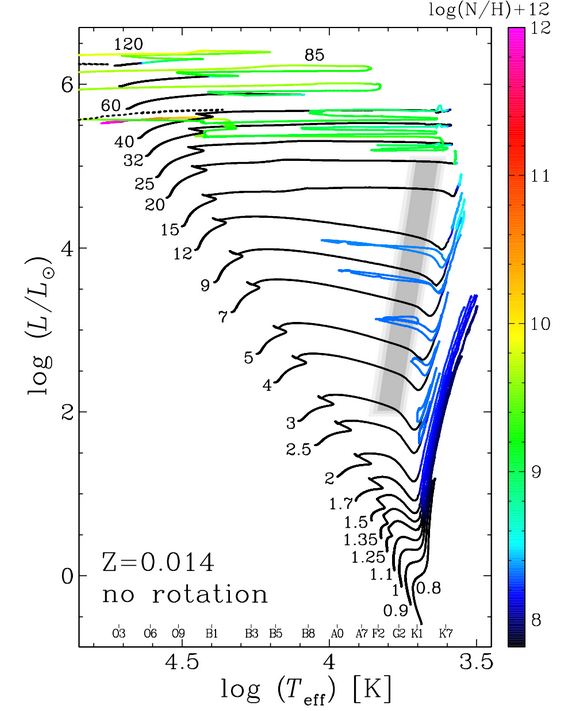
\includegraphics[width=0.65\textwidth]{intro/HRD}
 \caption[Hertzsprung-Russell diagram (HRD) of stars]{
Hertzsprung-Russell diagram (HRD) displaying the surface temperature (increasing to the left) against luminosity of stellar evolutionary models in the mass range
0.8~$<$~M/M$_{\odot}<$~120 taken from
\protect\citet{2012A&A...537A.146E}.
Each line represents a model, at Solar-like metallicity computed without stellar rotation, with an initial mass given on the left hand side (the start) of the evolutionary models.
Models are highlighted based on their nitrogen enhancements.
The MS is displayed on the left hand side of the evolutionary tracks where stars spend most of the lives.
Later stages in evolution are where the tracks evolve towards the left of the diagram (cooler temperatures).
 \label{fig:HRD}}
\end{figure}


During core hydrogen-burning, stars more massive than 1.1\,M$_{\odot}$ fuse hydrogen to helium through the carbon-nitrogen-oxygen (CNO) cycle.
In this case, convection is induced owing to the large temperature gradient established as a result of the high temperature dependence of the rate of the CNO cycle (T$^{14}$).
As a result of convective mixing, the core can be described as homogeneous during the hydrogen-burning phase~\citep{2012sse..book.....K}.
Convection is an important feature of this stage of evolution as it increases the MS lifetime by increasing the amount of material available for fusion.

Some of the main issues with the current theory of convection are characterising the size of the convective overshoot region and the effects of semi-convection on stellar evolution.
Convective overshooting acts to increase the mixing of material beyond the convective boundary, within a stable region.
As a convective cell is accelerated towards the boundary of the convective layer, its momentum carries the cell beyond this region into a region of convective stability.
This has several consequences for the evolution of the hydrogen-burning phase, which are direct results of convective overshooting increasing the amount of fuel available for consumption within the convective core.
How large an evolutionary effect convective overshooting produces is not well constrained.

Convective overshooting is characterised by the parameter $\alpha$ in units of the local pressure scale height ($H_{P}$)~\citep{2012sse..book.....K}.
% What is the local pressure scale height?
Various authors have placed constraints upon $\alpha$ by using observational techniques including, for example, measuring the width of the main sequence~\citep{Schroder97,Brott11}.
These studies (along with many others) find values of $\alpha$~=~0.1--0.6~\citep[a recent example is][finding $\alpha = 0.335$]{Brott11}.

Semi-convection is also an issue for more massive stars.
This is because, in massive stars, opacity is dominated by electron scattering~\citep{b:Bohm-vitense92.v3}.
Semi-convection is named as such because of a discrepancy between two different criterion for convection.
This situation arises outside a fully convective zone where a chemical gradient ($\nabla _{\mu}$) is established.
Semi-convection acts to smooth out the chemical gradient outside the fully convective regions.
% [This is not a good explanation of semiconvection!]
% What implications does semi-convection have for massive stars?
% Why does semi-convection only occur in massive stars on the MS?
%% In massive stars the opacity is dominated by electron scattering
%%
%% convection occurs if the radiatve temperature gradient exceeds the adiabatic temperature gradient


As the star evolves and more hydrogen is consumed, the mass of the convective core decreases~\citep{2012sse..book.....K}.
Eventually, the star consists of a pure helium core surrounded by a hydrogen-burning shell.
The maximum mass of the helium core, with respect to the total stellar mass is determined by the Sch\"onberg-Chandrasekhar limit
(q$_{SC}\geq\frac{M_{c}}{M_{tot}}$; usually derived as q$_{SC}\sim$~0.1), above which an inert helium core is unstable to gravitational collapse.
In stars in the mass range 3~$<$~M/M$_{\odot}<$~12, the Sch\"onberg-Chandrasekhar limit is usually reached at the end of the hydrogen-burning phase~\citep{b:SalarisCassisi05}.
At this point, the helium core collapses, increasing the core temperature and density sufficiently that core helium-burning can occur, halting the collapse in the process.
In more massive stars ($>$12\,$M_{\odot}$), core helium-burning can smoothly proceed without the need for core collapse, as the central temperature in these stars is sufficiently high (10$^{8}$\,K).

During this phase of evolution hydrogen-burning proceeds within a shell outside the core.
For stars which exceed the Sch\"onberg-Chandrasekhar limit, during core contraction the outer hydrogen envelope will expand owing to the \textquoteleft mirror principle\textquoteright ~of shell fusion.\footnotemark
\footnotetext{This principle is not well understood, but its effects appear to be a universal feature of shell fusion.}
As the outer envelope expands, the effective temperature decreases.
In Figure~\ref{fig:HRD}, the star moves to the right (towards redder colours) where massive stars evolve into the RSG phase and lower mass stars become red giant branch stars.
This phase of evolution proceeds on a Kelvin-Helmholtz timescale, which for a 7\,M$_{\odot}$ star is around 5~$\times$~10$^{5}$\,yr~\citep{2012sse..book.....K}, i.e. incredibly short on an evolutionary timescale.
The short timescale on which this evolutionary phase proceeds accounts for the observed Hertzsprung gap.
The evolution towards the red is halted as core helium-burning switches on.

In massive stars above 12\,M$_{\odot}$, core helium-burning is thought to ignite when the star appears as a blue supergiant (BSG)~\citep{Meynet11,2012A&A...537A.146E,Langer12,Saio13}.
The redward migration of BSG stars is dictated by an intermediate convective zone~\citep{Meynet11} present in the atmosphere of the star, and is more gradual than the redward evolution of less massive stars.
Stars more massive than around 40\,$M_{\odot}$ never become RSGs~\citep{Massey03,Meynet11,2012A&A...537A.146E} and hence, there is a peak luminosity of RSGs in any given population~\citep{1979ApJ...232..409H}.
As these massive stars evolve towards the red edge of the HR diagram, their luminosities approach that of their Eddington luminosities; this induces large mass loss episodes.
As a result, these stars halt their evolution towards the RSG phase and evolve towards the blue and consequently into Wolf-Rayet (WR) stars
\citep{2007ARA&A..45..177C, Vink09}, see 60\,M$_{\odot}$ track and above in Figure~\ref{fig:HRD}.

% For a 10M$_{\odot}$ star, core helium-burning proceeds for around 4Myrs~\citep{b:SalarisCassisi05}.
As suggested above, in specific cases, not all of the helium-burning phase is spent as a RSG.
The length of time spent during the RSG phase depends upon how core helium-burning ignites.
If a star begins its helium-burning lifetime as a BSG and subsequently evolves into the RSG phase, naturally, the length of time spent as a RSG will be shorter.
In addition to this, stars with masses in the range of 25~$<$~M/M$_{\odot}<$~40 are thought to evolve back from the RSG phase to the BSG phase while still burning helium in their cores~\citep{2012A&A...537A.146E}.

This evolution of massive stars between the BSG and RSG phase seeds the idea that stars in these stages of evolution will fall into two categories:

\begin{enumerate}
    \item stars which begin helium-burning in the RSG or BSG phase, or,
    \item stars which begin helium-burning in a different evolutionary state and have since evolved into either the RSG or BSG regime.
\end{enumerate}

Distinguishing these objects observationally is challenging.
\cite{Saio13} used radial pulsations to distinguish between models of BSGs, which \textquoteleft roughly agree\textquoteright ~with observations of NGC 300 and in the Galaxy.
However, an analogue to this has not been identified in RSGs.
\cite{2012A&A...542A..79C} argued based on the nitrogen enrichment of their population of observed BSGs that these stars are in the process of evolving toward a RSGs phase.
% Convection has a big role to play here.
%% Stellar models based on the Schwartzchild criteria for convection spend more time in the blue compared to models based on the Ladaux certeria~\citep{SalarisCassisi05}
% More about mass loss from BSGs

Regardless of how extended the external envelopes in these stars are, core helium-burning proceeds in an identical manner.
Helium burning in general proceeds through the triple alpha process, via the reaction, 3$\alpha$~$\rightarrow$~$^{12}$C~+~$\gamma$.
However, as the number density of $^{12}C$ increases, the reaction $^{12}$C($\alpha+\gamma$)$^{16}O$ is of increasing importance, although the exact rates at which these reactions proceed is not well constrained.
This process of nuclear burning is highly temperature sensitive (even more so than the CNO cycle); therefore, a convective core is once again induced.
In addition to this, massive red helium-burning stars also have large outer convective envelopes~\citep{2012sse..book.....K}, which means the star appears near the Hayashi limit for a fully convective star in the HR diagram.
The convective envelope dominates the evolution of all but the most massive RSGs (30~$<$~M/M$_{\odot}<$~40) which do not not appear as close to the Hayashi limit as their lower mass counterparts~\citep[see Figure 1 in][]{Saio13}.

At the end of the core helium-burning phase, a massive star contains a carbon/oxygen core surrounded by a helium-burning shell, which is in turn surrounded by a hydrogen-burning shell.
At this point, the situation in the core now resembles that of the stage before core helium-burning.
An inert carbon/oxygen core contracts and heats up which ignites the core fuel.
Stars with initial masses greater than around 8\,M$_{\odot}$ are able to fuse carbon in their cores in a stable fashion.
In order for lower mass stars to do so, a degenerate carbon core is required.
Whether or not stars are able to begin core carbon-burning in a stable manner is usually the physical basis for distinguishing between ``intermediate'' and ``high'' mass stars.
During this process, carbon fuses to form an unstable form of $^{24}$Mg which then decays through three channels:

\begin{enumerate}
    \item $^{24}$Mg$^{*}\rightarrow ^{23}$Mg$+n+\gamma$,
    \item $^{24}$Mg$^{*}\rightarrow ^{20}$Ne~+~$\alpha+\gamma$,
    \item $^{24}$Mg$^{*}\rightarrow ^{23}$Na~+~$p+\gamma$.
\end{enumerate}

Oxygen does not fuse at this stage of the evolution of the star and therefore the length of time a star spends fusing carbon depends strongly on the amount of carbon processing present in the helium-burning phase (namely, the reaction $^{12}$C($\alpha+\gamma$)$^{16}O$).

Once the carbon fuel has been exhausted in the core, shell carbon-burning proceeds.
The cycle of core contraction with new core reactants begins and subsequent neon-, oxygen- and silicon-burning in the core follow~\citep{Woosley02}.
As each new fuel in the core is exhausted, subsequent shell burning follows.
Fusion reactions cease with $^{56}$Fe as fusion reactions beyond this point are no longer energetically favourable.

Eventually, this leads to an \textquoteleft onion structure\textquoteright
~star, with an inert iron core surrounded by layers of lighter elements fusing in shells.
These fusion reactions proceed on such a short timescale that the outer envelope does not have the time to react to the changing conditions in the core.
This effectively \textquoteleft freezes out\textquoteright ~the outer envelope and the spectral type of the star does not change significantly during this period~\citep{Meynet11}.

% subsection life_cycle (end)

\subsection{Death} % (fold)
\label{sub:death}

Massive stars ($>$8\,M$_{\odot}$) end their lives as core-collapse supernovae (CCSN).
These violent explosions are responsible for distributing elements synthesised within massive stars during their nuclear-burning lifetime, as well as during the explosion event.
Observationally, CCSN are classed as type II, type Ib and type Ic.\footnotemark
\footnotetext{Type Ib and type Ic are often grouped as type Ibc, as the differences between these two types are difficult to distinguish~\citep[for example see][]{Eldridge13}.}
The classification of supernovae (SNe) is based on their optical spectra, specifically on the appearance of spectral features such as hydrogen and helium.

There are several different types of CCSN which occur as a result of the different conditions present in the cores of massive stars.
For an in depth review see~\cite{Janka12}.
For the purpose of this literature review, it will suffice to mention the four main CCSN channels: electron-capture SNe, iron-core SNe, gamma-ray burst SNe and pair-instability SNe.
This review will focus on iron-core SNe in particular.

Iron-core SNe account for the majority of observed CCSN~\citep{Smartt09,Janka12,Eldridge13}.
This type of SNe are produced by massive stars which have initial masses above $\sim$9\,M$_{\odot}$~\citep{Poelarends08}.
As mentioned in the previous section, massive stars conclude their nuclear-burning lifetimes with inert iron cores.
Owing to a lack of energy generation, the core contracts and heats up.
As the temperature reaches 10$^{10}$K, photons in the core of the star now have enough energy to photo-dissociate iron-group elements into $\alpha$ particles.
The increasing density forces electrons into nuclei and free protons, creating a neutron rich environment.
As densities approach nuclear density, core contraction halts as a result of the repulsive force of the strong interaction~\citep{Janka12}.
The in-falling outer layers crash into the core and the resulting shock-wave disrupts the entire star and produces the SN.

The exact mechanism which produces the SN explosion is subject to intense research, the subtleties of which will not be covered in this literature review.
Recently, two extensive review articles~\citep{Janka12, Burrows13} have been published on the subject giving a more in depth and complete overview of the subject.

In recent years, many SN progenitors have been discovered by reviewing extensive archival data available in the Local Group as well as through extensive dedicated SN surveys.
These studies (or a quick review of the Central Bureau for Astronomical Telegrams (CBAT) list of SNe\footnotemark) reveal that type II-P SNe are by far the most numerous type of CCSNe ($\sim$ 60\%) and RSG stars are firmly established as their progenitors~\citep[][and references therein]{Smartt09}.
\footnotetext{http://www.cbat.eps.harvard.edu/iau/cbat.html}
However, CCSN are observed in a variety of different types and hence, RSG stars are not the only type of massive star which can end their lives as SNe.
Figure~\ref{fig:SNe-Smartt} illustrates the many possible channels towards SNe; this includes RSGs, BSGs, WRs and recently luminous blue variable (LBV) stars are being established as a part of this list~\citep[e.g.][]{Smartt09, Groh13}.

 \begin{figure}
 \centering
 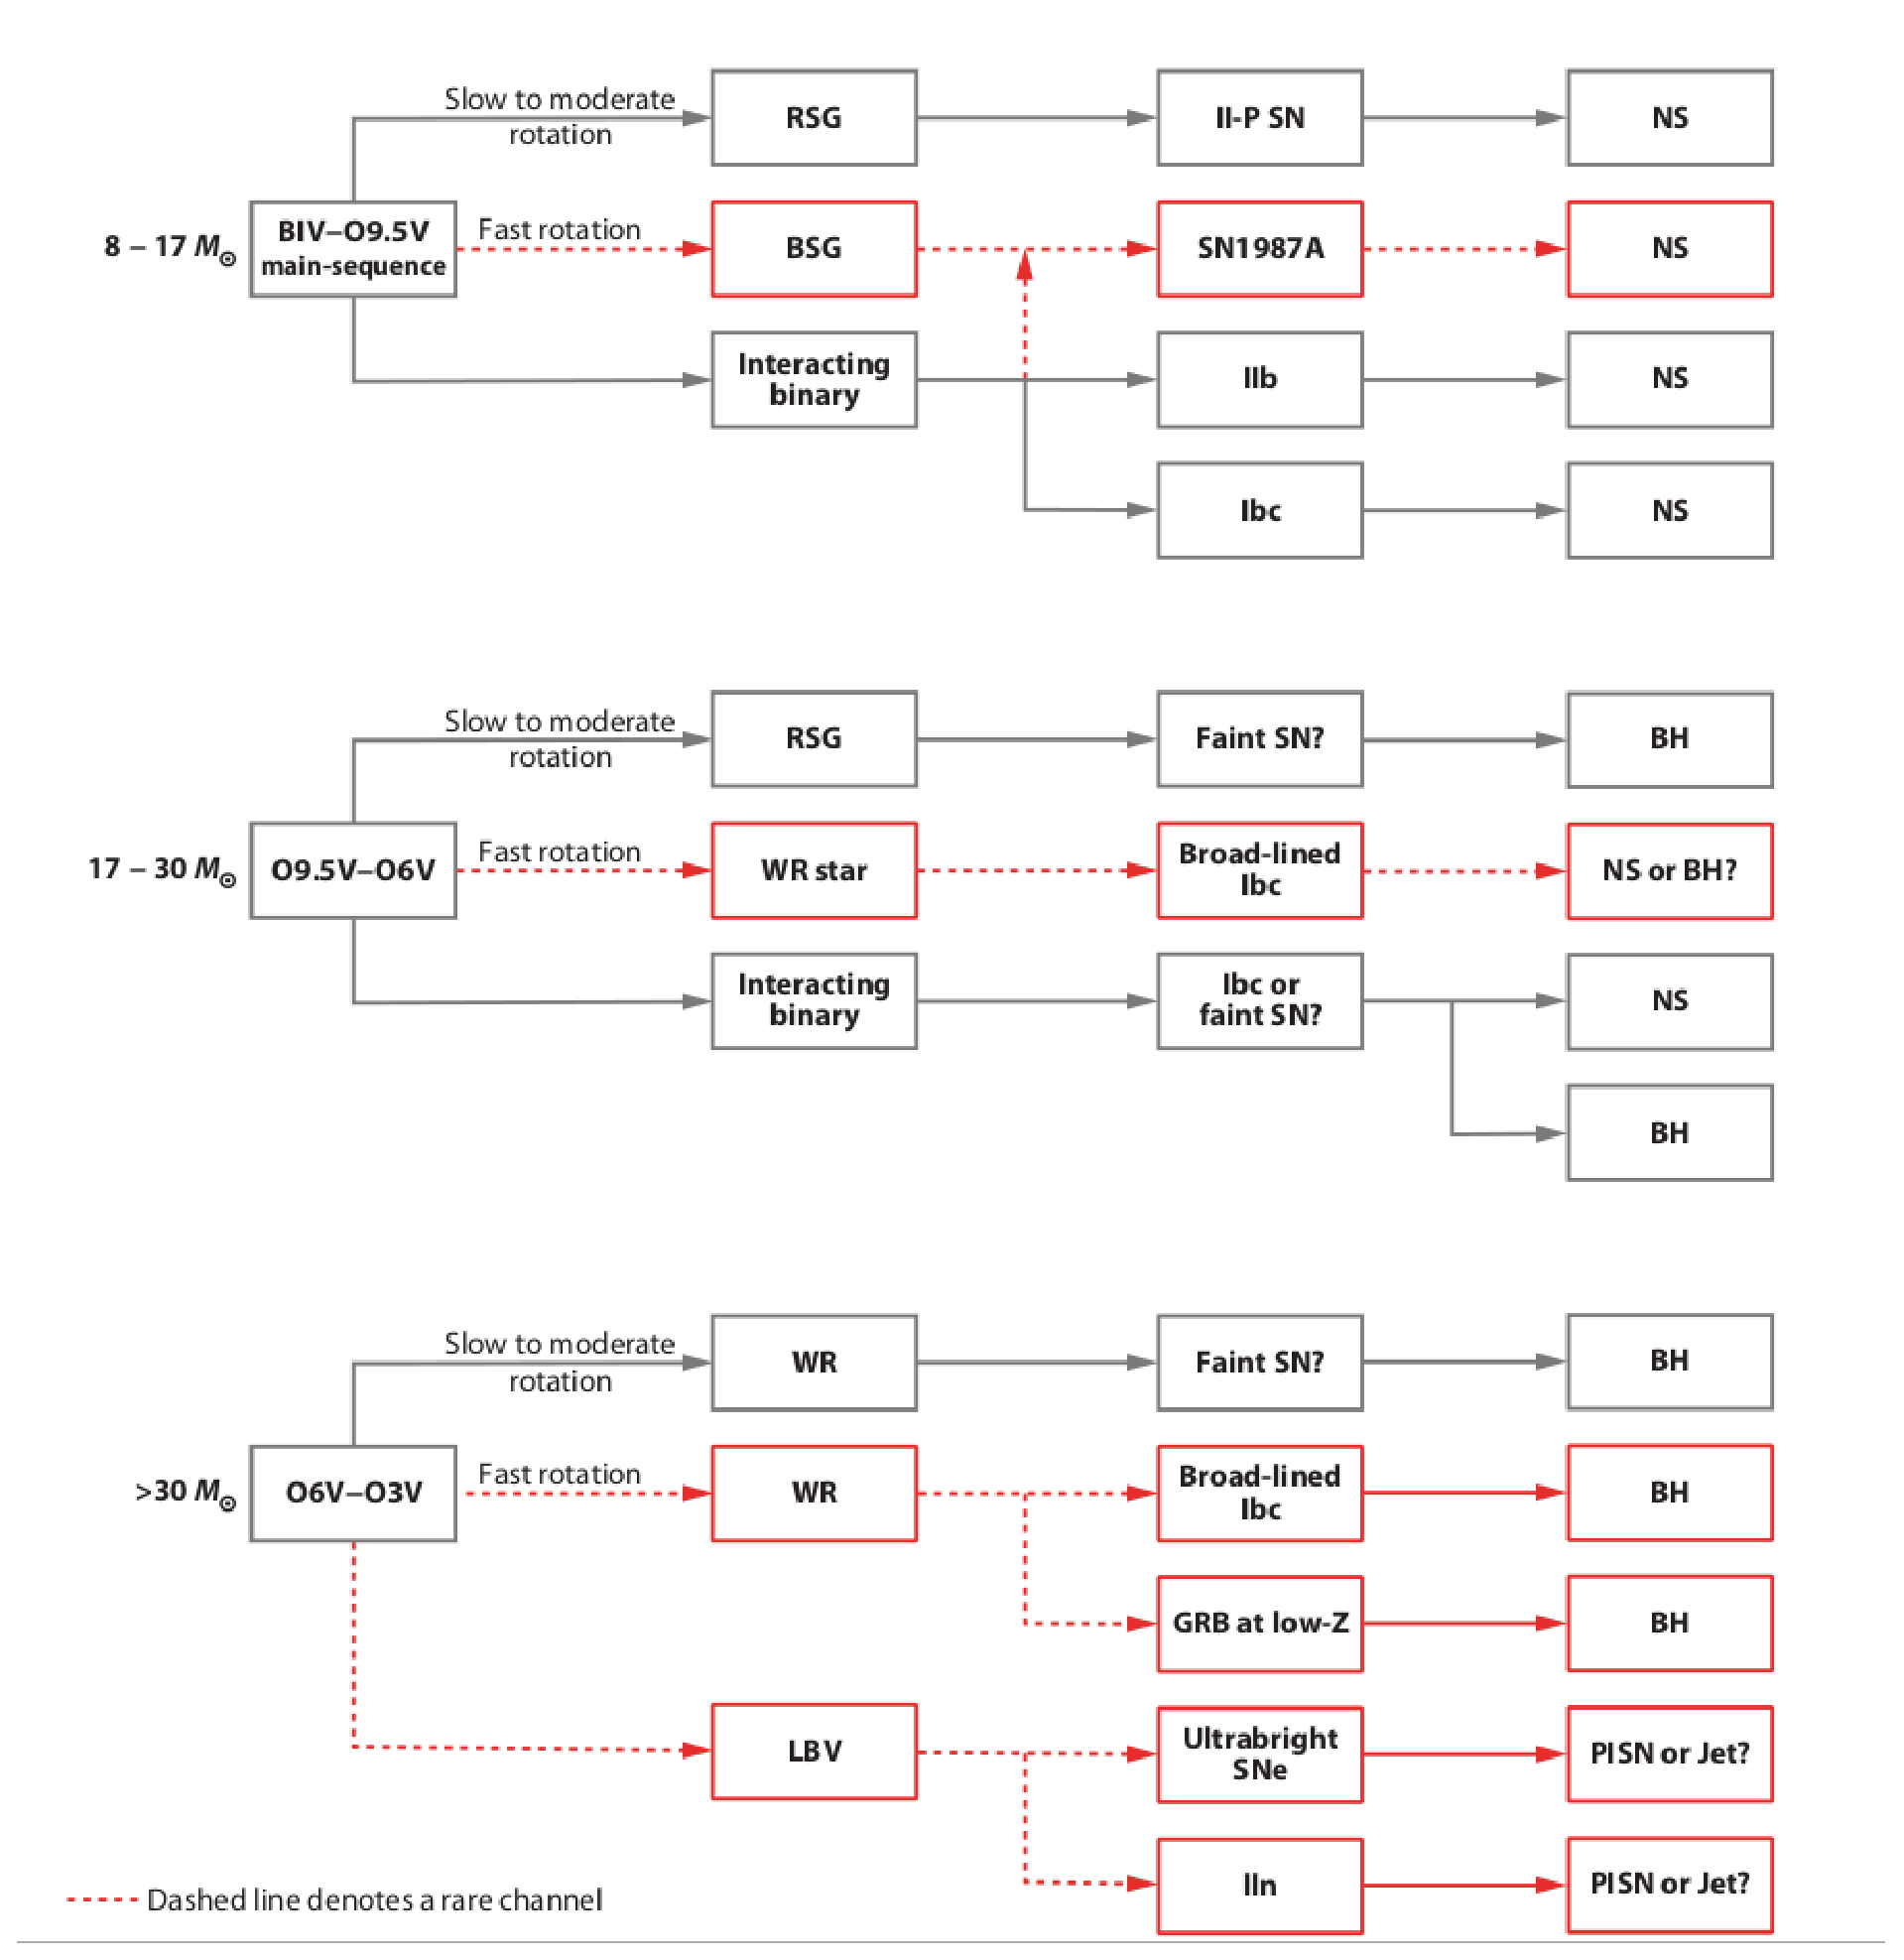
\includegraphics[width=0.65\textwidth]{intro/Smartt09fig12}
 \caption[Endpoints of massive stars]{The evolutionary diversity of the end points of massive stars and their associated observed SN classification. Figure reproduced from~\cite{Smartt09}. Acronym definitions: RSG, red supergiant; BSG, blue supergiant; LBV, luminous blue variable; WR, Wolf-Rayet; NS, neutron star; BH, black hole; GRB, gamma-ray burst; PISN, pair-instability supernova.
 \label{fig:SNe-Smartt}}
\end{figure}

% subsection death (end)
% section the_life_of_a_red_supergiant (end)

\section{Observations of RSGs at Home and Abroad} % (fold)
\label{sec:rsg_observations}

Red supergiant (RSG) stars are massive, bright, evolved stars located in recent star-forming environments.
As mentioned above, any star with an initial mass 8~$<$~M/M$_{\odot}<$~40 is expected to spend a portion of its life cycle as a RSG~\citep{2000A&A...361..101M,Massey03, 2007ARA&A..45..177C, Meynet11}.
As RSGs are so luminous, these objects can be studied in external star forming galaxies supplemented of course by more detailed studies of individual stars within our own Galaxy.
However, before one can study a RSGs they need to accurately identified and classified. In Section~\ref{sub:selection_of_rsgs} I deal with how this can be achieved, where I then go on to highlight some of the key observational results from Galactic and extragalactic studies of RSGs in Section~\ref{sub:galactic_and_extragalactic}.

\subsection{Identification and Classification of RSGs} % (fold)
\label{sub:selection_of_rsgs}

The classification of stars is based on the morphology of their spectra, with particular focus upon the absorption lines of hydrogen and other elemental features such as helium and calcium.
RSG stars have spectral type K or M, classified as such based on the appearance of strong molecular lines arising from their cool atmospheres.
Additionally, cool main sequence dwarfs and evolved giant stars also have spectral type K or M.
To distinguish between these populations of stars, luminosity is taken into account.
The luminosity of a star ($L$) is given by the equation,

\begin{equation}
    L = 4\pi R^2\sigma_{SB}T_{\rm eff}^4
\end{equation}

\noindent where $R$ is the radius of the star, $T_{\rm eff}$ is the effective temperature of the star and $\sigma_{SB}$ is the Stefan-Boltzmann constant (which in Chapter~\ref{ch:janal} is defined later as one of the fundamental equations of a star).

For a given spectral type the effective temperature of a star is roughly constant, therefore, luminosity is dependent solely upon the radius of the star.
The largest and most luminous stars, the supergiants, are labelled as class~\1, giants as class~\3 and dwarf or main sequence stars, with the smallest radii and hence the lowest luminosity, as class~\5.

In general, spectral features which are sensitive to luminosity are directly related to the physical size of the star rather than a product of the luminosity.
Supergiants have large extended atmospheres; hence, their radii are considerably larger than the more compact dwarfs and giants.
This distinction in physical size of stars results in various characteristic spectral features which are used to determine luminosity class.
In the optical regime, there are various different luminosity class indicators.
For K-type stars, the ratio of the Y\,\2 (4376\,\AA) line with Fe\,\1 (4383\,\AA) or the morphology of the Ca\,\2 H and K lines (for early K-type stars) are some of the most prominent~\citep{b:GrayCorbally}.
While for M-type stars, a system of molecular TiO lines centred on 5000\,\AA ~or the negative luminosity effect of the Ca\,\1 (4226\,\AA) line are clear indicators of luminosity~\citep{b:GrayCorbally}.
In the infrared, the 0-0 band of the CN molecule is the main luminosity discriminator at $\sim$1.1\,$\mu$m for both K- and M-type stars~\citep{b:GrayCorbally}.


% I want to include a section about why these lines change with luminosity class but I'm struggling to find reasons ...
%These features are sensitive to luminosity for a many different reasons. For example, the CaII H \& K lines in supergiants display broad wings, whereas in dwarfs and giants, the lines are narrower.
%Diminishing Stark effect is more extended atmospheres~\citep{b:GrayCorbally}

%Eg. lower densities and pressures cause atomic species with low ionisation energies to be pushed more towards an ionised electron + ion

Distinguishing between dwarfs, giants and supergiants for a given spectral type is important as these stars are different in terms of their stage of evolution and mass.
RSG stars are young, evolved stars which are fusing helium or heavier elements in their cores.
In contrast, dwarf M- and K-type stars are low mass, old stars which are still in the core hydrogen fusion stage.
Giant M- and K-type stars are evolved stars of intermediate mass and intermediate age currently on the asymptotic giant branch (AGB).
The exact divide between AGB stars and RSGs stars is, like all classification sequences which attempt to bin a continuous range of data, somewhat ambiguous and great care must be taken to separate these classes of stars.

The most effective method of classifying stars is to obtain spectroscopic observations which cover some of the important diagnostic luminosity indicators with sufficient resolution to distinguish between unique observational signatures.
However, spectroscopic observations are expensive.
In the absence of spectroscopic observations, the selection of stars in general is often done using broad band photometry.
% This section will describe some of the various methods used to isolate a population of stars using magnitudes derived from broad band filters.
Isolating a population of stars using photometric selection techniques is important as photometry can target a large number of stars with a relatively small amount of observing time which can be used to optimise follow up observing programmes to target specific types of stars.

The appearance of colour-magnitude diagrams (CMDs) are often used to isolate particular types of stars.
Colour is defined as the difference between two magnitudes at different wavelengths.
Essentially, a colour traces the shape of the spectrum of the star (which is defined to first order by the effective temperature), and the brightness of a star in a given filter (magnitude) can be used to approximate luminosity.
Therefore, theoretically a CMD should allow for the separation of a population of stars with distinct luminosities and temperatures.
The situation is simplified in the case of the RSGs as these stars are expected to be among the brightest in a stellar population.
However, this method assumes that the sample consists purely of one population of stars at a fixed distance.
When a population of stars is distributed over a significant range of distances, a brighter star with a larger distance is degenerate with a nearby fainter star.
In addition, dust extinction can affect the colours of stars which can cause a star with a bluer colour which is significantly extincted by dust to appear as a redder star with a smaller contribution from extinction.

An example of an optical CMD of NGC\,6822 is given in Figure~\ref{fig:CMD}.
In this figure one can see large scale structures arising as different types of stars distinguish themselves based on their properties.
However, this figure also demonstrates some of the potential issues with using these types of diagrams to select targets.
The large feature at $B-V \sim$~1.0 is attributed to foreground contaminants.
RSGs are found on this figure at the tip of the reddest plume with $B-V >$~1.5.

\begin{figure}
 \centering
 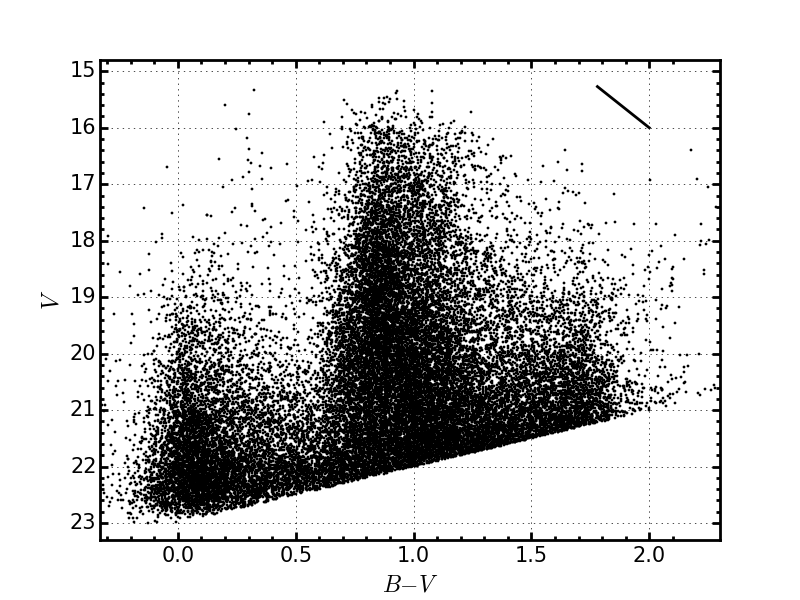
\includegraphics[width=0.65\textwidth]{intro/NGC6822_bv_CMD}
 \caption[Optical colour-magnitude diagram of NGC\,6822]{Optical colour-magnitude diagram (CMD) of NGC\,6822, in which the absolute V-band magnitude M$_{V}$, (corrected to the distance of NGC 6822) is plotted against $B-V$ colour.
This figure illustrates how CMDs can be used to separate stars based on spectral type. Redder colours indicate later spectral types.
This figure also demonstrates that CMDs have inherent degeneracies between different populations of stars.
 \label{fig:CMD}}
\end{figure}

To break the degeneracy between luminosity and distance as well as distance and reddening, one can use colour-colour diagrams.
Using multiple colour diagnostics can isolate stars based on more than just spectral type and absolute magnitude.
\cite{1998ApJ...501..153M} show that at a given $V-R$ colour, the $B-V$ colour is sensitive to the surface gravity of a star.
Therefore, RSGs can be isolated from other stars of similar $B-V$ colours owing to their low surface gravity.
An example of such a colour-colour diagram is shown in Figure~\ref{fig:CCD} where one can clearly see the distinction between low surface gravity RSG stars (with slightly redder $B-V$ colours) and the dwarf high surface gravity stars.

\begin{figure}
 \centering
 \includegraphics[width=0.65\textwidth]{intro/N6822_bvr}
 \caption[$B-V$, $V-R$]{Optical colour-colour diagram of NGC 6822. This figure illustrates the surface gravity dependence of the $B-V$ colour at a given $V-R$ colour where the dashed line separates the population of RSGs from stars with similar spectral types.
 \label{fig:CCD}}
\end{figure}

The selection of RSGs is typically done using a $B-V$, $V-R$ colour-colour diagram as this diagram has had much success in selecting RSGs and is known to contain a small number of contaminants.
However, a potential issue with these diagrams as we move to extragalactic systems, which at the time of writing has not been quantified, is that RSGs are known to reside in dense regions and/or clusters with many bluer, younger stars.
When viewing these stars in the optical, the colours from RSGs could potentially be contaminated to bluer colours by the blue stars which also reside nearby.
In a $B-V$, $V-R$ diagram, this contamination would affect the completeness of the population of RSGs selected.
As stated, this is not quantified and would require a comparison between the $B-V$, $V-R$ selection method with another known selection method and an analysis of the locations of the potentially contaminated RSG stars.
A potential solution to this problem would be to select RSGs based on their near-IR colours, which is where these stars are brightest and hence would be less subject to contamination to nearby blue objects.
% This argument could be reversed and in the near-IR we could push blue stars towards our RSG targets. Would this be a problem?

Working in the near-IR, authors have used the J, J-K CMD~\citep[e.g.][]{2000ApJ...542..804N,2006A&A...452..195C,Neugent12} to select red stars (RSGs and asymptotic giant branch (AGB) stars) and much work has been done in identifying contaminants and the parameter space where individual populations reside in~\citep{2006A&A...452..195C}.
As mentioned above, the main contaminants with this selection method are foreground dwarfs.

In the mid-IR, authors have used the [3.6] - [4.5] CMD to distinguish between RSGs and various types of AGB stars~\citep{2006AJ....132.2034B,2014A&A...562A..75B,2015A&A...584A..33B,2015ApJ...800...51B,2015A&A...578A.100W} and using these longer wavelengths has proved a useful tool to study the dust properties of these cool stars.

% subsection selection_of_rsgs (end)


\subsection{Galactic and Extragalactic studies} % (fold)
\label{sub:galactic_and_extragalactic}

The intrinsic brightness of RSGs, particularly in the near-IR, makes these stars popular candidates for observations within and beyond the Galaxy.
Studies of Galactic RSGs are used to test theories of stellar evolution and estimate fundamental stellar parameters such as radii, masses and distances.
Galactic RSGs are also a natural starting point for extragalactic studies of larger populations of RSGs.
Extragalactic observations have identified populations of RSG stars in a large range of galaxies within the Local Group and (in rarer cases) out to larger distances~\citep[e.g.][]{Elias85,Humphreys86, Massey06, 2007AJ....134.2474M, Groenewegen09,Massey13}. % how do I put "table 1 in massey"?
These studies provide important results on RSGs in different environments.

% \subsubsection{Fundamental Parameters in Galactic RSGs}\label{Galactic RSGs}

As RSGs are intrinsically rare within stellar populations given their masses and, consequently, short lifetimes.
Within the Galaxy there are examples of prominent individual RSGs such as $\alpha$ Orionis (Betelgeuse), VY Canis Majoris and Antares which have gained considerable attention for countess years\footnotemark.
In addition to individual RSGs there are examples of Galactic (and extragalactic) young massive clusters (YMCs) whose light output are dominated by RSGs and contain tens of these objects.
Examples include, the {\it h} and $\chi$ double cluster and more recently discovered clusters such as  red supergiant clusters 1, 2 and 3~\citep[RSGC01, RSGC02, RSGC03][respectively]{2006ApJ...643.1166F,2007ApJ...671..781D,2009A&A...498..109C} and Alicante 8~\citep{2010A&A...513A..74N}, each contain a large concentration of RSGs.

\footnotetext{\cite{2003UppOR..59...51R} suggested that cave markings in Germany dating to around 30\,000\,BCE represented the constellation Orion, of which Betelgeuse is part of.}

Research into individual Galactic RSGs typically is concentrated on estimating structural or dynamical properties of atmospheres or on circumstellar material surrounding these stars where one can test detailed stellar evolutionary and atmospheric models against high quality observations~\citep[e.g.][]{2014A&A...561A..15C}.
A useful reference to obtain an overview of what research is being conducted on individual RSGs in the galaxy is~\cite{2013EAS....60.....K}, the conference proceedings for an entire workshop centred around Betelgeuse.

Observations of Galactic RSGs reveal that they have large mass-loss rates
\citep[10$^{-(6\pm 1)}$\,M$_{\odot}$\,yr$^{-1}$;][]{Danchi94, Richards13,2016AJ....151...51S} and extended circumstellar environments~\citep{Smith01,2014MNRAS.437L...1W} which may contain masers~\citep[e.g.][]{Schuster06,2012ApJ...744...23Z}.
Mass loss during this phase of evolution is critical for the understanding of subsequent evolutionary stages as well as understanding SN progenitors.
For example, the remnant of SN 1987A displays loops which are thought to have originated in mass loss events during the RSG phase of evolution of its progenitor star~\citep[][and references therein]{Humphreys13}.
Galactic RSGs act as an important sample to study and understand the mechanisms of mass loss, as extragalactic observations are unable to resolve the structure which can be seen in nearby Galactic stars.

One of the main uncertainties with studies of these nearby stars are the relatively poorly constrained distances e.g. Betelgeuse~\citep[197\,$\pm$\,45\,pc;][]{Harper08} and VY CMa
\citep[$\sim$1300\,$\pm$\,120\,pc;][]{Wittowski12,2012ApJ...744...23Z} which are attributed to large variations of surface structure~\citep{2011A&A...528A.120C}.
In order to (partially) remove the distance uncertainty problem, RSGs can be observed in Galactic clusters of known distances~\citep[e.g.][]{Humphreys78, Mel'Nik95}.
%% MS fitting, observe spectral type and fit cluster onto a HR diagram to estimate the absolute magnitude, distance modulus
This technique is useful to study large populations of RSGs which can be used to test theories of star formation and models of RSGs and their atmospheres.

% \subsubsection{Extragalactic Studies and Results}\label{extragalactic RSGs}

Extragalactic studies of RSGs are advantaged in that it is possible to accumulate large samples of RSGs, at a fixed distance, with which to test stellar evolution theories and estimate stellar parameters.
By using the different environments available in the Local Group, studies of extragalactic RSGs can probe a wide range of host galaxy parameter space.
For example, M31 (Z$>$1.0Z$_{\odot}$ in the central regions), a massive, metal-rich spiral galaxy and the Wolf-Lundmark-Melotte (WLM; Z=0.1Z$_{\odot}$), a dwarf irregular, metal-poor galaxy, both contain a significant population of RSGs.

Through an analysis of RSGs in different metallicity environments, some authors have reported that the average spectral type of a RSG population is dependent upon metallicity~\citep{Elias85, MasseyOlsen03, 2012AJ....144....2L}, where lower metal abundances give rise to earlier average spectral types.
In addition to this, RSGs can be used to measure abundances in Local Group galaxies, which yield important results by mapping metallicity gradients.
This work had typically been done using high-resolution spectra at near-IR wavelengths~\citep{Cunha07, Davies09a,Davies09b}.
However, in order to optimise these studies,~\cite{2010MNRAS.407.1203D} adapted a method for determining the chemical properties of BSG stars in the optical
\citep{2008ApJ...681..269K,2010AN....331..459K}, to RSGs in the near-IR.

These studies exploit that fact that even though RSGs are evolved objects, for massive stars, the hydrogen-burning lifetime is short~\citep[just over 25\,Myr for a 8\,M$_{\odot}$ star and consequently shorter for higher mass stars][]{2012A&A...537A.146E}.
Therefore, although RSG stars are in an evolved state, they are in actual fact still remarkably young stellar objects ($<$30\,Myr old, as that subsequent generations of nuclear fusion are significantly shorter than the time scale for hydrogen fusion).
Given the fact that these stars are very young, in general they have not had the time to travel a significant distance from their birth place.
Therefore, their chemical composition must closely match that of their surrounding environment (accounting sufficiently for a certain amount of nuclear processing).
This means that studies of RSGs in extragalactic environments can probe the present day metallicities of their surrounding environments which are comparable to H\,\2 region studies (see Section~\ref{sec:chemical evolution}).

In addition to their young ages, RSGs are also intrinsically attractive objects to study at near-IR wavelengths.
% There are many reasons to study RSG stars at near-IR wavelengths.
From a technological point of view, the next generation of optical-infrared telescope (e.g. European Extremely Large Telescope, Thirty Metre Telescope, James Webb Space Telescope) will be optimised for studies in the near-IR; therefore, in order to make the best use of these facilities in the future, we must refine and optimise our observational strategy on facilities today.

There are also many intrinsic properties of RSGs themselves which make  which make them desirable objects to study in the near-IR.
As noted earlier, RSGs are among the most luminous objects in any star-forming galaxies and given their cool atmospheres the peak luminosity for RSGs is $\sim$1.1\,$\mu$m.
Coupled with this is the fact that near-IR observations are less affected by dust obscuration which is important as, by definition, RSGs are dusty objects, owing to their high mass-loss rates.
Therefore, near-IR observations are the optimal wavelength to observe RSG stars at large distances.

Measurements of the temperatures of RSGs have also provided insight through using observations of extragalactic RSGs in the near-IR.
The temperatures of RSG stars have been subject to debate for many years which again is likely a product of their complex atmosphere and surface structure.
There are many methods by which to estimate the effective temperature of a RSG star.
The most popular of which is to fit the spectral energy distribution (SED) of the star with 1D model atmospheres~\citep{Levesque05,Levesque06}.
However,~\cite{2013ApJ...767....3D} demonstrated that observations fitting models around the BVRI region, where molecular TiO lines dominate the absorption, result in a systematically lower temperature compared with fitting the line-free continuum regions of the SED.
This is due to the fact that the TiO molecular line forms higher in the atmosphere of the star than the continuum.
This means that fitting the TiO region and assuming that the best fitting effective temperature is representative of the entire SED is not a good assumption.
\cite{2013ApJ...767....3D} advocate using the entire SED \textit{except} those regions dominated by the TiO absorption features.
Estimating temperatures of extragalactic RSGs will be an important test for stellar evolution models and an excellent way in which to test models at different metallicities and in different environments.
\cite{2015ApJ...803...14P} highlighted the interesting result that the temperature of RSGs in different environments appears to be insensitive to the metallicity of the RSG. (This result is presented and commented upon in Chapter~\ref{ch:ngc6822})

In summary, I have highlighted some of the ways in which one can take measurements of RSGs in both at home (in our own galaxy) and abroad (in external galaxies).
Owing to various factors I have demonstrated that studies in the near-IR can have a significant impact on the understanding of RSGs and their environments.
RSGs and massive stars in general play a key role in distributing material throughout their host galaxies and understanding the physical process which affect these environments is key to furthering studies of galactic chemical evolution.



% section observations_of_red_supergiant_stars_at_home_and_abroad (end)

\section{Chemical Evolution of Galaxies as probed by red supergiant stars} % (fold)
\label{sec:chemical evolution}


The evolution of galaxies is a vast area of study which can be broadly split up into three main fields: dynamical, thermal and chemical evolution.
%In reality these topics depend upon each other, but given certain crude approximation can to an extent be studied independently.
The chemical evolution of galaxies governs the origin and distribution of elements within the host galaxy.
This evolution principally depends upon galaxy and star formation where
the initial distribution of the chemical elements is defined by how the galaxy is formed.
Star formation acts to alter these quantities by creating, redistributing and removing chemical elements from the interstellar medium (ISM).

The lowest mass stars remove elements from the ISM by storing their gas and never evolving off the MS.
Stars massive enough to evolve off the MS eject some mass during an AGB phase, but subsequently end their lives by removing elements from the ISM as passively cooling white dwarf stars.
%These stars could also end up as Type Ia SNe
More massive stars undergo large amounts of mass loss during all phases of their evolution and end their lives by exploding as CCSNe, both of which act to alter the chemical composition of their surrounding gas clouds.

All three of these processes are important to take into account when studying how galaxies chemically evolve over time.
However, quantifying contributions from these quantities is an involved process, complicated by a minefield of caveats and uncertainties.

Extragalactic observations of fundamental properties of galaxies play important roles in refining theories of galaxy formation and evolution.
The mass-metallicity relationship~\citep[MZR;][]{Lequeux79} of galaxies relates two fundamental parameters of galaxies.
The stellar mass represents the amount of gas which star formation has removed from the ISM, whereas the present day galaxy metallicity represents how star formation has altered the initial ISM.
Various authors have shown that galaxy mass is proportional to metallicity~\citep{Tremonti04, Maiolino08,Kewley08}.
This relationship can be interpreted by considering multiple factors.
In low-mass galaxies, outflows and SNe have a greater affect on the amount of material ejected from the host galaxy into the intracluster medium, owing to their shallower potential wells~\citep[e.g.][]{Tremonti04}.
Additionally, low-mass galaxies represent an early stage in Galactic evolution and hence, these galaxies have not had time to process their gas into stars.
As the host galaxy evolves, subsequent episodes of star formation increase the metal content of the galaxy~\citep[e.g.][and references therein]{Maiolino08}.

MZR observations have typically relied upon ratios of strong oxygen emission lines (usually [O\,\2], [O\,\3] relative to H$\beta$) from H\,\2 regions to estimate metallicities of individual galaxies.
This technique is used owing to its applicability over a large distance range:
\cite{2001MNRAS.323..887C} use this technique in nearby galaxies whereas~\cite{Maiolino08} estimate metallicity using this method in galaxies at z$>$3.
However, these measurements are known to be highly dependent upon the calibration method used~\citep{Kewley08,2008ApJ...681..269K,Bresolin09}.
In order to provide an independent calibration of this method, BSG stars have been used to determine metallicity and abundance gradients in external galaxies~\citep{Kudritzki12}.
In addition to using BSGs, this thesis describes and builds on a method which uses RSGs as abundance probes of external galaxies which can be used to calibrate the MZR by building up large numbers of observations of RSGs in external galaxies.

Independent calibration of the MZR is essential to study how galaxies chemically evolve.
The MZR has been shown to exist in the Local Universe as well as at earlier epochs within many different types of galaxies~\citep[e.g.][]{2011ApJ...730..137Z,2013ApJ...765..140A,2014ApJ...795..165S,2014MNRAS.440.2300C,2014MNRAS.437.3647Y,2015ApJ...799..138S} and is thought to be a ubiquitous property of galaxy formation.

% section chemical evolution (end)


\section{Motivation and Outline} % (fold)
\label{sec:motivation_and_outline}

This thesis aims to develop and expand the use of RSGs as abundance probes in external galaxies with the eventual goal of independently calibrating the MZR of galaxy evolution.
By using state-of-the-art model stellar atmospheres and high quality spectroscopic observations of RSGs, in this thesis I will demonstrate the ability of this analysis method to study large populations of RSGs in external galaxies, measuring not only fundamental stellar parameters in a wide range of different environments, but also using RSGs as probes of how metals are distributed within external galaxies.

In addition, this thesis forms the basis on which all studies of RSGs with the $K$-band multi-object spectrograph (KMOS) will be founded upon.
As I continue to learn about this instrument and make the most of the observations which have been obtained, I find that KMOS can not only be used for chemical studies of galaxies, but also to study the kinematics of massive populations within these galaxies.

RSGs have enormous potential to become important indicators of galaxy metallicity and this project has allowed me to become involved in the early phases of this project.
In addition, with the coming generations of facilities and the realisation that near-IR studies have unique insights and qualities, near-IR spectroscopy (in general) will also become an increasingly prominent tool in the toolbox of the astronomer.
Developing these analysis techniques and techniques of observation today is fundamental to make the best use of upcoming observatories.
I feel, this thesis has contributed significantly to this development.

This thesis is organised as follows.
In Chapter~\ref{ch:kmos} I describe the principles of spectroscopy and go on to describe KMOS, the instrument which is used extensively in this thesis, and some of the modifications which I have developed to obtain the best results from this instrument.

Chapter~\ref{ch:janal} outlines the underlying physics which is used when constructing stellar model atmospheres and describes the state-of-the-art models which are used to analyse RSG spectra.
This leads on to a description of the analysis technique which is used to measure stellar parameters of RSGs and tests this method on various different data sets.

Chapter~\ref{ch:ngc2100} describes KMOS observations of 14 RSGs within NGC\,2100, a YMC in the LMC, where the chemistry and kinematics of the star cluster are assessed.
Using the analysis routines described in Chapter~\ref{ch:janal} stellar parameters are estimated and compared to previous results. An upper limit to the line-of-sight velocity dispersion is measured for the cluster and the dynamical mass is estimated for the first time.
By combining the individual RSG spectra, I demonstrate that this analysis technique can be used to estimated the integrated properties of unresolved clusters at larger distances at LMC-like metallicity.

Chapter~\ref{ch:ngc6822} describes observations of 18 RSGs in NGC\,6822, dwarf irregular galaxy on the edges of the Local Group with a turbulent past.
I test different strategies for reducing this data and quantify the spatial variations in metallicity within this galaxy, finding intriguing evidence for an abundance gradient.
I demonstrate that using a simple, closed, chemical evolution model the young and old populations of NGC\,6822 are well explained. An important result as NGC\,6822 displays evidence for recent interactions.
In this chapter I also highlight the result that the temperature of RSGs does not depend upon the metallicity, something which is not predicted by evolutionary models.

Chapter~\ref{ch:ngc55} presents observations of 22 RSGs in NGC\,55, a large spiral galaxy outside the Local Group of galaxies.
Stellar parameters are estimated using the technique described in Chapter~\ref{ch:janal} and I discuss how to optimise the data reduction strategy to obtain results from a challenging data set.
Spatial variations in metallicity are examined and the evolution of NGC\,55 is commented upon.

Chapter~\ref{ch:mzr} provides a first look at the calibration to the MZR using RSGs in the Local Universe.
Using the results of the previous three chapters I estimate the MZR from three data points.

Finally, Chapter~\ref{ch:conclusions} presents concluding remarks and outlines future directions.

% \bibliography{../journals,../books}

% section motivation_and_outline (end)
% \chapter{Spectroscopy and the {\it K}-band Multi-Object Spectrograph}
\label{ch:kmos}
\section{Opening Remarks} % (fold)
\label{sec:opening_remarks}
KMOS warrants an individual chapter in this thesis as all of the spectroscopic observations are from this instrument.
This chapter initially describes the basic design of a spectrograph and outlines some of the more commonly used spectroscopic techniques in Section~\ref{sec:intro_to_spec}.
I then move on to describe integral field spectroscopy, a more complex spectroscopic technique, in Section~\ref{sec:IFS}.
I then go on to describe KMOS in Section~\ref{sec:KMOS} and the KMOS data reduction process in Section~\ref{sec:3Ddata}.
Finally, I conclude the chapter in Section~\ref{sec:conclusions}.


% section opening_remarks (end)

\section{Introduction to Spectroscopic Techniques} % (fold)
\label{sec:intro_to_spec}

Spectroscopy is the study of the dispersion of light into its constituents and has been at the forefront of astronomy for roughly the last 200 years.
Sir Isaac Newton demonstrated the principles of spectroscopy (and coined the term ``spectrum'') using light from The Sun in his seminal ``Opticks'' work~\citep{b:Newton}.
By using the groove spacings on a diffraction grating, Thomas Young first quantified the wavelengths of different colours of light~\citep{1802PTRSL.92.12Y}.
The simple set-up of a spectrograph, which has - more or less - been used since the early spectroscopic experiments, consists of five basic elements:


\begin{enumerate}
    \item Slit
    \item Collimator
    \item Dispersive element
    \item Camera
    \item Detector
\end{enumerate}

A simple spectrograph is illustrated in Figure~\ref{fig:spectrograph}.
In Newton's demonstration he used a small hole in his window blinds as a slit and a screen as a detector.
The slit in modern spectroscopic observations can take various forms.
The most widely used type of slit, in modern observations, is long-slit spectroscopy.
Using a long slit, a spectrum is taken for each spatial pixel along the length of the slit.
This is demonstrated in Figure~\ref{fig:long-slit}, where the final panel shows that each pixel illuminated within the slit produces a spectrum.
This can be thought of a 2-dimensional spectroscopy, which is particularly useful when attempting to take a spectrum of an extended object
(rather than a point source).

\begin{figure}
 \centering
 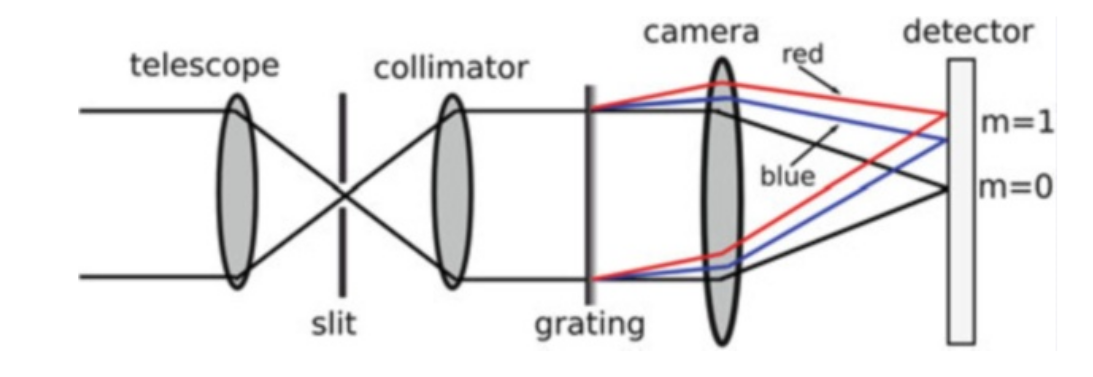
\includegraphics[width=0.65\textwidth]{kmos/Lawrence-spectrograph}
 \caption[Simple Spectrograph]{A simple spectrograph detailing the five basic elements a spectrograph posseses: slit, collimator, dispersive element, camera and detector.
 Credit:~\cite{2014amcg.book.....L}.
 \label{fig:spectrograph}}
\end{figure}

\begin{figure}
 \centering
 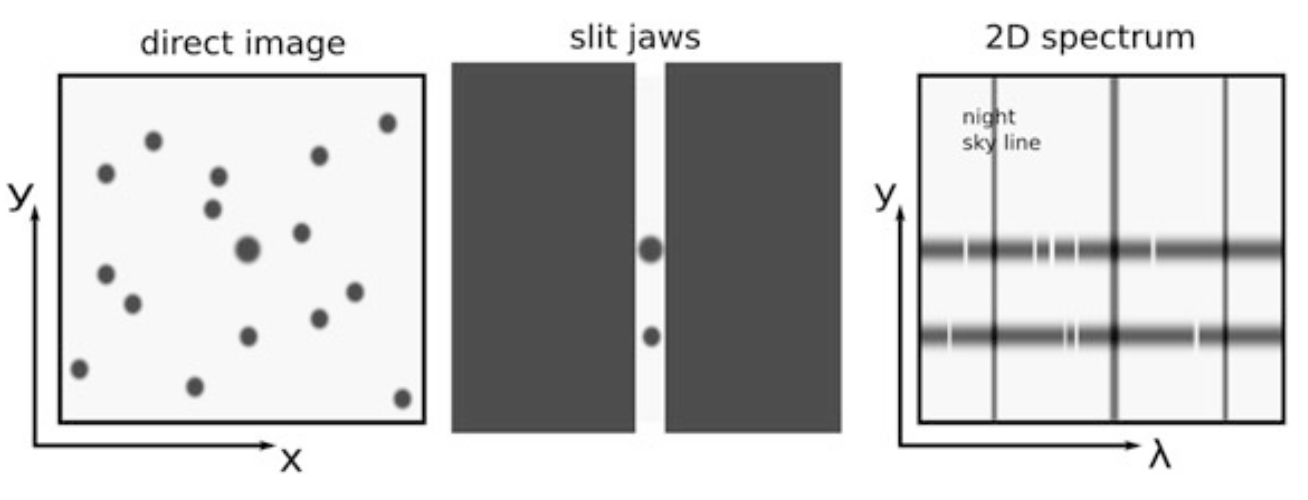
\includegraphics[width=0.65\textwidth]{kmos/Lawrence-long-slit}
 \caption[Long-slit Spectroscopy]{Three panels demonstrating long-slit spectroscopy.
 The left panel shows what an image of the FoV would see.
 The central panel illustrates that the long slit selects only the slit width in the $x$-axis, while including the full $y$-axis range.
 The right panel shows that for each pixel in the $y$ direction, a spectrum is obtained.
 Credit:~\cite{2014amcg.book.....L}.
 \label{fig:long-slit}}
\end{figure}

An alternative to using a long-slit to remove contamination from other sources is to use a small hole or fibre to select the target flux.
By precisely drilling a hole in a metal plate, a slit is created which can be used to select the target flux.
One of the advantages of using this method is that more than one object can be selected for a single exposure.
By creating multiple slits within a single plate, spectroscopy of multiple objects can be obtained where contamination from other sources is minimised.
An improvement to this method was to use optical-fibres positioned within the holes (e.g. Figure~\ref{fig:multi-obj}).
The fibres could then be led to an instrument which was not directly attached to the telescope, which has the advantage that the instrument will not suffer from the changing gravitational force as the telescope moves.
In addition, the conditions within the instrument room can be controlled.
This is particularly important for near-IR spectrographs and detectors.

However, using a plate with several holes drilled into it has some drawbacks.
These include the time in which it takes to create the slit mask, the lack of flexibility while observing and the operational costs of creating a new mask each time a different field is to be observed~\citep{1986SPIE..627..118P}.
These reasons, in addition to improved computing power, led to the development of instruments which were able to automatically position fibres~\citep{1982SPIE..331..289T}.
Most modern fibre-fed spectrographs have automatic fibre-positioning technology which is broadly split up into two approaches.

\begin{enumerate}
    \item Each fibre has a magnetic button attached and a single robot is charged with moving each fibre sequentially.
    This is an effective method to place large numbers of fibres, but does however, take a significant length of time for each configuration.
    \item Each fibre is mounted upon a computer-controlled arm.
    This method is generally less time consuming.
\end{enumerate}

As a variant on the five basic elements of a spectrograph, slitless spectroscopy is also a feasible option which is not discussed in detail here.
For a thorough overview on slitless spectroscopy see~\citet{2014PhDT.........C}.

\begin{figure}
 \centering
 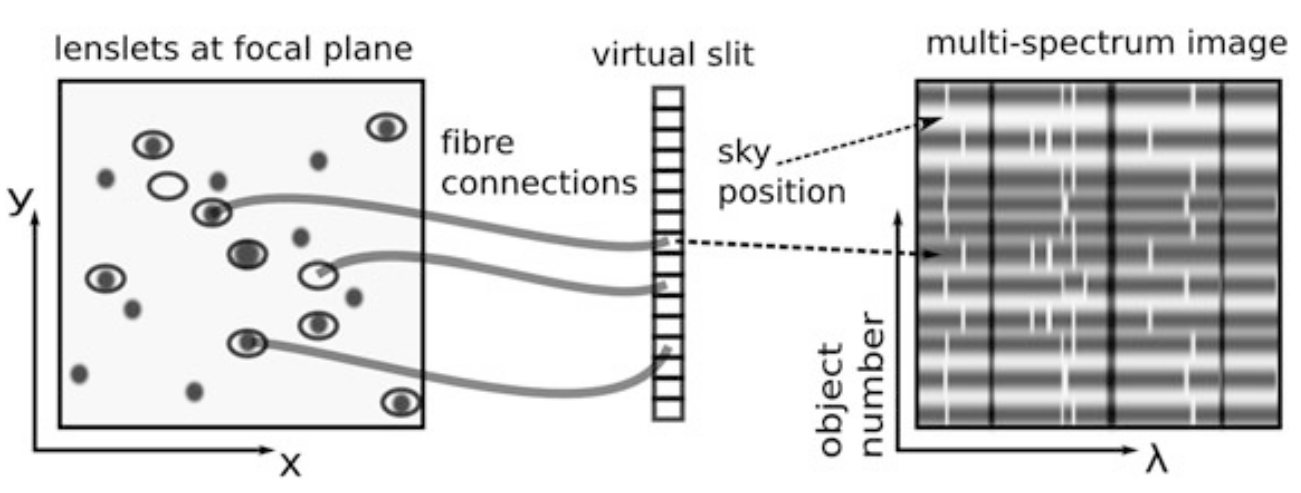
\includegraphics[width=0.65\textwidth]{kmos/Lawrence-multi-object}
 \caption[Multi-object Spectroscopy]{Three panels demonstrating multi-object spectroscopy.
 The left panel shows what an image of the FoV would see.
 The central panel illustrates that each fibre in this simple multi-object spectrograph can be positioned at any point throughout the field of view and is rearranged into a pseudoslit.
 The right panel shows that for each pixel in the $y$ direction, a spectrum is obtained.
 Credit:~\cite{2014amcg.book.....L}.
 \label{fig:multi-obj}}
\end{figure}

A key element to any spectrograph is the dispersive element.
In Newton's original experiments this took the form of a glass triangular prism.
A prism disperses light based on the wavelength dependence of the refractive index of glass: differential refraction.
This produces a low-resolution spectrum spanning a large spectral range.

Typically in modern spectrographs the dispersive element is a diffraction grating.
A diffraction grating consists of a reflective surface with many parallel grooves.
These grooves act as slits and disperse the light which is then combined on the detector through interference using the same principles as a double slit experiment.
Figure~\ref{fig:doubleslit} shows the interference pattern for monochromatic light striking two slits of width $a$ with separation $d$ at a wavelength $\lambda$.
By increasing the number of slits the fringe maxima remain stationary while becoming narrower and more intense.
The angular positions ($\theta$) of the fringe maxima are,


\begin{figure}
 \centering
 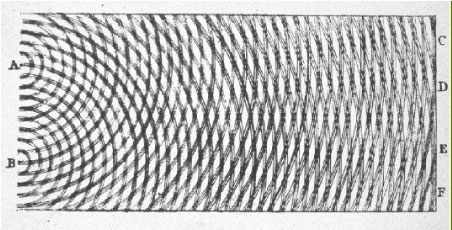
\includegraphics[width=0.65\textwidth]{kmos/youngslits}
 \caption[Double slit interference pattern]{A double slit interference pattern from Thomas Young's original experiments.
 \label{fig:doubleslit}}
\end{figure}


\begin{equation}
    sin\,\theta = \frac{m\lambda}{d},\label{eq:a}
\end{equation}

\noindent where $m$ is an integer and refers to the fringe order ($m$~=~0 for the central undispersed peak).
As the number of secondary peaks depends upon the number of rulings $N$, the angular positions of the zero positions also depend upon $N$,

\begin{equation}
    sin\,\theta = \frac{m'\lambda}{Nd}.\label{eq:b}
\end{equation}

\noindent Therefore, the angular width of the principle maximum between the first two zero positions ($\Delta\theta$ or $W$) is obtained by defining,
\begin{equation}
     W = \Delta m'\frac{d\theta}{dm'},\label{eq:c}
\end{equation}

\noindent and by differentiating equation~\ref{eq:b},

\begin{equation}
    W = \frac{2\lambda}{Nd\,cos\,\theta}.\label{eq:d}
\end{equation}

\noindent The Rayleigh Criterion states: ``Two point sources are regarded as just resolved when the principal diffraction maximum of one image coincides with the first minimum of the other''~\citep{1880MNRAS..40..254R}.
By the application of this criterion one can define the spectral resolution in terms of the angular separation as,

\begin{equation}
    W = \frac{\lambda}{Nd\,cos\,\theta}.\label{eq:e}
\end{equation}

\noindent which does not depend upon the fringe order.
Typically, the spectral resolution is quoted in terms of the smallest wavelength which can be separated in the spectrum.
This is given by converting the angular width into the corresponding wavelength width using $\Delta\lambda = \Delta\theta\,d\lambda/d\theta$ which gives,

\begin{equation}
    \Delta\lambda = \frac{\lambda}{Nm},\label{eq:f}
\end{equation}

\noindent more commonly quoted as the ratio of the operating wavelength to the spectral resolution,

\begin{equation}
    R = \frac{\lambda}{\Delta\lambda} = Nm,\label{eq:g}
\end{equation}

\noindent where $R$ is typically termed the spectral resolving power (or incorrectly as the resolution).

Separation of the spectral orders is an important consideration in diffraction grating spectroscopy which is usually taken into account using a broadband blocking filter to limit the spectral range to a single order only.
In principle, higher spectral resolving power can be obtained by viewing higher spectral orders, however, both the intensity of the spectra and spectral range are diminished.
Typically low spectral orders are used in astrophysical observations.

Diffraction gratings have many intrinsic advantages over glass prisms when used for quantitative spectroscopy however they are used in tandem for some applications.
Echelle spectrographs working in higher orders for larger resolving powers make use of an additional dispersive element, which is often a prism, to spatially separate different orders so that they can be simultaneously recorded on the detector.

% If I can find an expample of this I can re-include it ...
% Alternatively, prisms can be arranged to counteract the dispersive properties of a grating.
% This allows the instrument to operate using an imaging mode without moving any of the essential optical elements (i.e. the camera).

Even though prisms are used rarely in modern astronomical spectroscopy they still have some important application.
The upcoming James Webb Space Telescope (JWST) near infrared spectrograph NIRSpec will contain a prism (in addition to several diffraction gratings) to obtain low-resolution spectroscopy of a very large spectral range (0.6--5.3\,$\mu$m).

% section introduction_to_spectroscopic_techniques (end)

\section{Integral field spectroscopy} % (fold)
\label{sec:IFS}

The overall goal with integral field spectroscopy (IFS) is to obtain a spectrum of everything (targets and their surroundings) within a given field of view (FoV).
This concept builds on the idea that a long-slit spectrograph obtains spectra for targets within the extent of the slit.
A natural extension of this technique would be to use a long-slit spectrograph to obtain a spectrum for each pixel within a 2-D FoV on the sky.

There are many intrinsic advantages to having a specifically designed instrument to perform this task rather than simply repeating observations with a long-slit spectrograph.
These advantages include,

\begin{enumerate}
    \item slit-losses are eliminated,
    \item accurate target acquisition is not required,
    \item the target position can be recovered from data,
    \item reduced radial velocity errors from positional issues in the slit when comparing target and reference object,
    \item the velocity field is recovered without biases.
    % \item IFS always optimally samples object point spread function (PSF).
\end{enumerate}

In addition, potentially the most compelling argument is that to perform IFS with a long-slit spectrograph one is required to take $N$ exposures all of length $t_{exp}$, however, using IFS, a spectrum for each spaxel is obtained with a single exposure. Therefore efficiency on-sky is increased.


\subsection{Techniques of integral field spectroscopy} % (fold)
\label{sub:techniques_of_integral_field_spectroscopy}

IFS may be achieved using a variety of different and novel methods.
Potentially, the simplest of these is (and most cost effective in the short term) is to take multiple exposures using an existing spectrograph over a small FoV.
Another, conceptually simple, approach is to take photometric data of the same field using multiple narrow-band filters which can be stitched together to create effectively low-resolution spectra of a FoV~\citep[e.g. GTC-OSIRIS][]{2011PASP..123.1107M}.


There are three main techniques which are more commonly used to generate spectra over a 2-dimensional FoV.
A spectrograph specialised for integral fields adds an additional element to the five basic elements of a spectrograph outlined previously.
This additional element is an integral field unit (IFU) which acts to split up the image obtained by the telescope into elements or slices which are constructed into a slit and dispersed by the dispersive element.
The difference between the techniques is in the way in which they split up the image.
In this section I will detail each of these techniques in turn and conclude by providing a comparison between them.

A lenslet array splits the input image using a tight array of small lenses~\citep{1995A&AS..113..347B}.
The lenses then focus the light of each sub-field separately which are then dispersed.
This technique limits the length of the spectrum measured on the detector.
To improve this the spectra are tilted about the optical axis to minimise overlapping of spectra, which leads to inefficient packing of the resulting spectra on the detector (e.g. Figure~\ref{sec:IFS}).

Fibre arrays use a tightly packed bundle of fibre-optic cables to split the telescope image.
The fibres then reposition the image onto a linear slit.
Figure~\ref{fig:IFS} shows a cartoon of this process.
As the fibre cables are intrinsically cylindrical objects, much light is lost between fibres in the focal plane.
To minimise the light lost, this technique can be improved upon by using an array of lenses to focus the light from each element into the fibre, effectively combining this technique with the previous method.

The final technique is to use an image slicer to split the image from the telescope~\citep{1997SPIE.2871.1295C}.
Figure~\ref{fig:image_slicer} shows an image slicer used in the KMOS instrument.
An image slicer is a type of segmented mirror where each linear segment reflects light in a slightly different direction.
A second segmented mirror then arranges the images into a pseudoslit where it is then dispersed.
As~\cite{2006NewAR..50..244A} demonstrate, this method is intrinsically efficient as complete slices of the field are imaged by the detector.
In addition, this method is also particularly applicable for IR studies as the optical system consists mainly of mirrors which are easily cooled to low temperatures.
Drawbacks with this technique include that a large and complex optical system is required with a surface roughness ($\sigma$) of $\sigma \leq$~10\,nm in the IR.


\begin{figure}
 \centering
 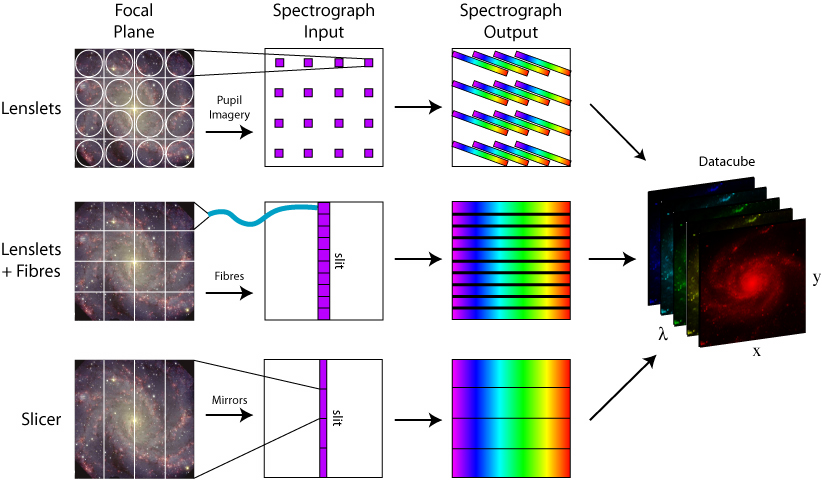
\includegraphics[width=0.65\textwidth]{kmos/ifu_designs}
 \caption[Integral Field Spectrosopic methods]{Three diagrams demonstrating the techniques of IFS
 Credit: M. Westmoquette, adapted from~\citep{2006NewAR..50..244A}.
 \label{fig:IFS}}
\end{figure}

\begin{figure}
 \centering
 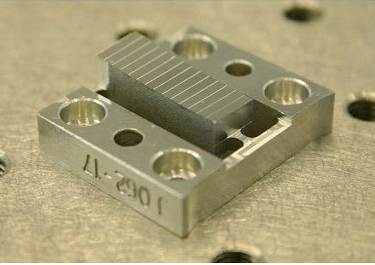
\includegraphics[width=0.65\textwidth]{kmos/kmos-image-slicer}
 \caption[The KMOS image slicer]{An image slicer from one of the arms used in the KMOS instrument.
 An image slicer is a type of segmented mirror which, in this case, slices the image into 14 different segments where each segment focuses the light in a slightly different direction.
 KMOS has 24 of these image slicers.
 Note: Image retrieved from the ESO website: https://www.eso.org/sci/facilities/develop/instruments/kmos.html
 \label{fig:image_slicer}}
\end{figure}


\cite{2006NewAR..50..244A} perform a detailed theoretical comparison between these three techniques and conclude that using an image slicer to split up the telescope image is the most efficient, by a considerable margin.
Using fibres or lenslet arrays give similar performances, although lenslet arrays are easier to construct.
Image slicer instruments, however, are the most complicated to construct owing to their complex optical systems.

% subsection techniques_of_integral_field_spectroscopy (end)


% section integral_field_spectroscopy (end)


\section{The {\it K}-band Multi Object Spectrograph} % (fold)
\label{sec:KMOS}
KMOS is a second generation instrument on the Very Large Telescope (VLT), Chile which completed its design review in 2008 and completed commissioning in April 2013.
As its name suggests, KMOS is a multi-object spectrograph operating at near-IR wavelengths (providing coverage from 0.8--2.5\,$\mu$m), which hosts 24 IFUs.
Therefore, KMOS can be described as a multi-object integral field spectrograph.

KMOS was designed specifically to provide spatially-resolved spectroscopy, while allowing multiple spectroscopic observations at near-IR wavelengths and was constructed by a consortium of UK and German institutes in collaboration with the European Southern Observatory (ESO).
The final design of KMOS boasts 24 configurable arms, each hosting an IFU with a 2.8"~$\times$~2.8" FoV which can be placed at user-specified positions within a 7.2' FoV.
These IFUs anamorphically magnify their individual sub-field onto one of the 24 advanced image slicers which partition each sub-field into 14 slices each with 14 spatial pixels.
Therefore one KMOS IFU obtains 14$\times$14 contiguous spectra in a single exposure.

The optical design of KMOS includes a three-fold symmetry about the Nasmyth optical-axis (see Figure~\ref{fig:kmoslight}).
Each segment is designed to receive the light from 8/24 of the configurable IFUs which is then passed to a cryogenic spectrograph containing five diffraction gratings (IZ, YJ, H, K and HK).
Therefore, KMOS has three quasi-identical spectrographs which can be independently configured and set up.

\begin{figure}
 \centering
 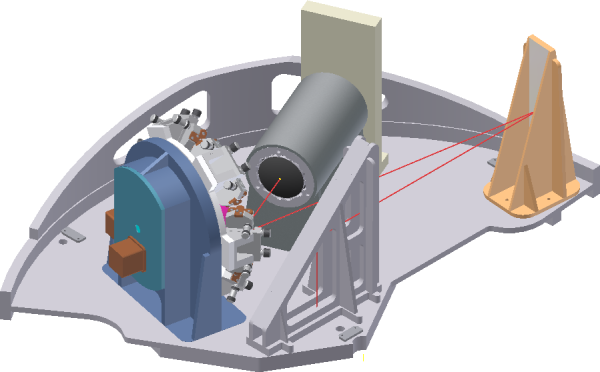
\includegraphics[width=0.65\textwidth]{kmos/kmos-spectrograph}
 \caption[The KMOS light path]{The light path for a KMOS spectrograph demonstrated by the solid red line.
 The IFU entrance slit is located underneath the baseplate.
 The light path comes from the slit entrance and is redirected by the fold mirror toward the collimator (right, highlighted in yellow), where the light then is directed to the grating (left, housed in the blue filter wheel containing all 5 gratings) which disperses the light in camera barrel which finally focuses the light onto the detector (where the detector mount is in beige).
 \label{fig:kmoslight}}
\end{figure}

KMOS was designed with specific science goals which revolved around the case for spatially resolving the structure in galaxies across a large range of redshifts and environments~\citep{2006NewAR..50..370S} and,
as the most-efficient near-IR multi-object spectrograph in the southern hemisphere,
KMOS has gained significant attention from the wider community.
Following successful commissioning runs KMOS underwent two science verification (SV) runs before being made available to the community for general observing in October 2013~\citep{2015IAUS..309...11S}.
Since then KMOS has been used to study many different science goals and has already had an impact in the fields of some of its key science drivers~\citep{2016MNRAS.456.1195H,2016MNRAS.456.4533M} as well as some intriguing results in other areas~\citep{2015A&A...584A...2F,2015MNRAS.453.3875P}

In addition, KMOS has been exploited as a multi-object spectrograph to study the metallicities of star-forming galaxies using RSGs as cosmic abundance probes~\citep{2015ApJ...805..182G,2015ApJ...812..160L,2015ApJ...803...14P}.
% This programme is described in detail~\ref{ch:janal}.
This thesis makes extensive use of KMOS and would not be possible without this state-of-the-art instrument.


% section the_instrument (end)

\section{Production of Three-dimensional Data Cubes} % (fold)
\label{sec:3Ddata}

The nature of IFS is to obtain spatial and spectral information for each pixel on a detector.
The final data product is, therefore, a three dimensional data cube consisting of two spatial and one spectral dimension.
Therefore, the goal of the data reduction and calibration process is to create this regularly-sampled data cube from (often) several raw detector images.

As mentioned, KMOS is arranged into three identical segments.
Each segment contains eight IFUs which are arranged to project data onto a single detector.
Each IFU contains an advanced image slicer which slices the field into 14 slices (see Figure~\ref{fig:image_slicer}) each of which contain 14 spatial pixels.
Therefore, one IFU produces 196 individual spectra which means a single detector contains information on over 1500 spectra.
An example of a raw data product with KMOS is illustrated in Figure~\ref{fig:kmosdata} and highlights that each IFU contains 14 spectra each of width 14 pixels on the detector.
This figure demonstrates how the dispersed spectra are arranged on the detector.

\begin{figure}
 \centering
 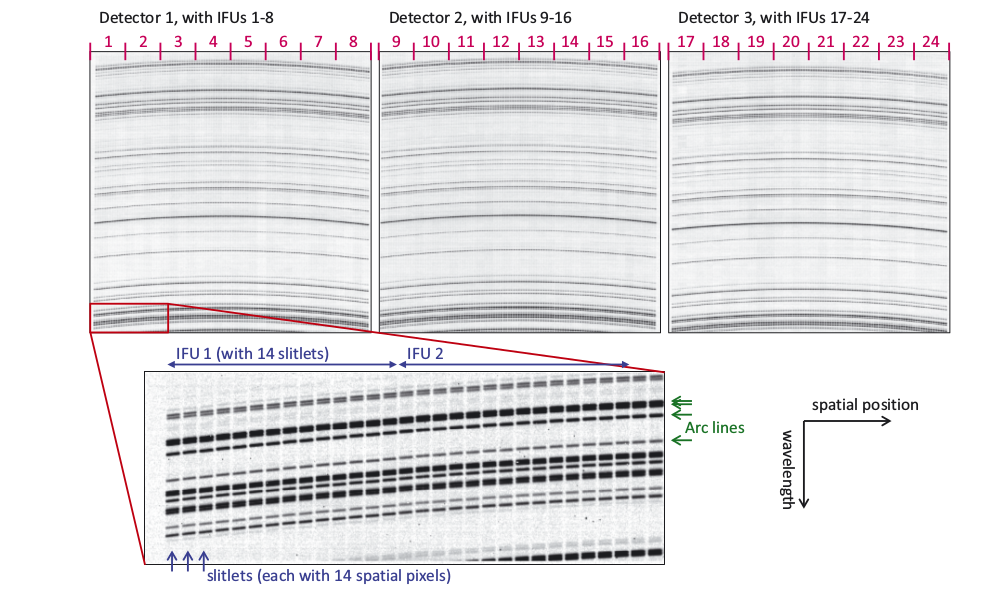
\includegraphics[width=0.65\textwidth]{kmos/kmos-data-Davies13}
 \caption[An example of KMOS raw data]{An example of a raw data product form KMOS taken from~\citet{2013A&A...558A..56D}. This figure  illustrates that in one frame, light is dispersed onto one of three detectors.
 Each detector records light from eight IFUs which is dispersed roughly in alignment with the $y$-axis on the detector.
 Each IFU contains 14 spectra with a width of 14 detector pixels and therefore the $x$-axis roughly corresponds to the spatial axis.\label{fig:kmosdata}}
\end{figure}

KMOS is designed so that on the detector, the y-axis roughly corresponds to the spectral axis.
However, on the detector there is no concept of spatial and spectral axes,
only information which can be calibrated and reconstructed into a regularly sampled cube with spatial and spectral axes.


\subsection{Calibration} % (fold)
\label{sub:calibration}

To calibrate KMOS data each value recorded by the detector must be assigned spatial and spectral information.
To do this one can use the projection of the light onto the detector, and the reliability of this projection, as a detailed diagnostic.
Slitlets are positioned on the detector to $\pm$\,1\,$\mu$m
\citep[roughly 1/18$^{\rm th}$ of a pixel;][]{2013A&A...558A..56D} and
the mean slit-width across the detector is 13.6\,$\pm$\,0.1\,pixels,
where the error quoted here is the standard deviation of the mean from all slitlets.
This pattern is so stable that subtle imprints of the opto-mechanical design of the instrument can be seen in the patterns~\citep[see Fig. 2 of ][]{2013A&A...558A..56D}.

The main factor that affects this pattern is the temperature of the spectrograph.
As with any IR instrument, the detector must be cryogenically cooled to minimise the effects of photons from the thermal background promoting electrons into the conduction band of the semi-conducting diode of the detector which are then confused with signal from the target.
For KMOS the detectors are cooled to $\le$~80\,K.
In addition to the cooling of the detector, the optical bench -- which houses the spectrographs -- is also cooled to $\le$~140\,K.
However, the temperature of the optical bench is not controlled and can therefore vary with the ambient temperature of the surroundings by several Kelvin which has a small, but significant, effect on the positions of the slitlet edges when the positions of the slitlets are compared between calibration frames and science frames (described below).
The implications of this potential temperature variation of the optical bench are that during calibration frames, the temperature must be within $\pm$\,1\,K of the science frames.

To make use of the pattern of the slitlets on the detector to calibrate the raw data, two types of calibration frames are obtained.
Flat lamp calibrations use a halogen lamp with a white-light spectral appearance to fully illuminate each slitlet and are used to calibrate the spatial positions of each detector pixel.
Arc lamp calibrations use halogen lamps which create a spectrum containing several diagnostic spectral features which are used to calibrate the wavelength of each detector pixel.
These calibration frames are then compared with the science frames to construct a three dimensional data cube for each IFU.
An example of a reconstructed IFU is given in Figure~\ref{fig:kmosIFU}.
This figure is a snapshot of the reconstructed IFU at a particular wavelength.

\begin{figure}
 \centering
 
\includegraphics[width=0.65\textwidth]{kmos/kmos-ifu}
 \caption[Example of a KMOS IFU]{An image of reconstructed KMOS IFU demonstrating, how each of the 14 slices of the field contains 14 pixels.
 This image is at a wavelength of 1.100\,$\mu$m.
 A spectrum is produced for each pixel and the current image is a snapshot at one particular spectral pixel.
 \label{fig:kmosIFU}}
\end{figure}

Calibration of the KMOS data can be split into three distinct processes:

\begin{enumerate}
    \item Flatfielding,
    \item Mapping data onto a regularly-sampled cube,
    \item Correction for atmospheric emission/absorption and instrument transmission.
\end{enumerate}

All of these processes are required to calibrate spectroscopic data in general, however, mapping the distortions of an instrument and transforming the data into a regularly sampled cube is necessarily an instrument-dependent approach and,
because of the complexity involved in arranging eight IFUs onto a detector, is the most important set-up in calibrating KMOS data.

Flatfielding is the process which corrects for the difference in response from detector pixels and is performed in a standard fashion using halogen lamps.
Flatfielding is also used to correct for variations in the illumination of the KMOS IFUs.
This is done directly using exposures from halogen lamps (lamp flats) and can be improved upon by using the twilight sky to illuminate the detector (sky flats).
Using the twilight sky is generally (not just for KMOS but within spectroscopy in general) preferred as the light path is identical to that of the science exposures.
However, observing in twilight conditions is extremely time dependent and in practice is difficult to undertake for an instrument as complex as KMOS.

To create the three dimensional data cube from KMOS raw data, a look-up table is created containing information relating each detector value with spatial and spectral locations.
This look-up table is implemented by creating three calibration files containing $x, y$ and $\lambda$ information for each pixel.
These calibration frames are created by making use of the repeatability of the pattern of the slitlets on the detector.
By fully illuminating the slitlets using the lamp-flat exposures the edge positions can be matched between the calibration and the science frames.
This provides the two spatial coordinates for each detector value.

To calibrate the wavelength of the each detector pixel one must illuminate the detector with a spectrum where the wavelength of each spectral feature is precisely known (i.e. the arc flats).
This is achieved with KMOS using a halogen lamp containing Neon and Argon where strong spectral features of known wavelengths cover the full detector range.
By identifying a few isolated spectral lines within these exposures, which are then traced across the length of the detector, a polynomial function is used to assign each pixel with a wavelength value.

As KMOS is a roughly three tonne instrument, the effects of flexure can be significant and are mainly caused by rotation of the instrument on the Nasmyth platform.
To account for this, calibration frames are taken at various rotator angles which are chosen to match the rotator angle of the science observations.
Using calibration files at a more appropriate rotator angle can make a reasonable correction to the most serious sources of flexure.


At this stage, all the information needed to create the three dimensional data cube is available in three calibration files.
This information is now used to transform the detector values onto a regularly sampled three dimensional data cube for each IFU.
It is necessary to perform multiple interpolations to the detector values, rather than simply rearranging these values, as -- in the frame of reference of the regularly sampled three dimensional data cube -- the detector values are irregularly sampled.
This is obvious from Figure~\ref{fig:kmosdata} which illustrates that the spectral and spatial axes are \textit{roughly} aligned with the $x$ and $y$ axes of the detector respectively.

There are, in principle, many different methods to create the data cube which affect the spectral and spatial resolution of the final data product.
The method which typically produces the highest quality data uses two (or three) one dimensional interpolations, the so-called ``cubic spline interpolation'' routine in the pipeline.
This method makes use of two properties of the IFUs:

\begin{enumerate}
    \item each slitlet is a straight line when projected onto the sky,
    \item the spacing across each slitlet is fixed and uniform (as a result of the properties of the image slicers).
\end{enumerate}

By exploiting these properties this method is able to assign each detector pixel an $x$, $y$ and $\lambda$ value.
This is achieved by -- using ii -- rearranging the detector values across each slitlet where no interpolation is necessary.\footnotemark
Subsequently a one dimensional cubic spline interpolation is performed along each slitlet, using i.
A final one dimensional cubic spline interpolation is performed in the spectral direction.
This method produces the best spectral resolution as well as giving highly consistent spatial resolution within each IFU.

\footnotetext{This is the case when the default sampling is used, when any other sampling is requested this step requires an additional interpolation performed using the cubic spline method.}


The final step in calibrating KMOS data is to take into account the effects of the Earth's atmosphere.
Observing from within the Earth's atmosphere affects the quality of the data in two different ways.
Intrinsically, when observing an astrophysical source through the Earth's atmosphere, each illuminated detector pixel contains a combination of source and sky photons.
Molecules and dust within the Earth's atmosphere scatter, absorb and emit light from the Earth and Moon which contaminates spectroscopic and photometric observations.
To account for this one typically attempts to observe a sky spectrum without any signal from the astrophysical source.
This usually takes the form of observing offset sky positions, where between each target exposure, sky targets are observed which are chosen to minimise contamination.
This results in an additional set of sky frames which are then used to calibrate the science frames using the same IFU in both science and sky exposures.
A simple example of the sky subtraction procedure is illustrated in Figure~\ref{fig:skysub}.
This figure shows that the signal from the sky is significantly larger than the signal from the object.
These sky frames are dealt with in the same manner as science frames in terms of calibration.
Typically, before the reconstruction of the three-dimensional data cubes however, the sky frame which is nearest in time to the science frame in question is subtracted.
% This correction can be improved upon by making small corrections to the sky cube using a sample of spatial pixels containing a smallest amount of target flux.

\begin{figure}
 \centering
 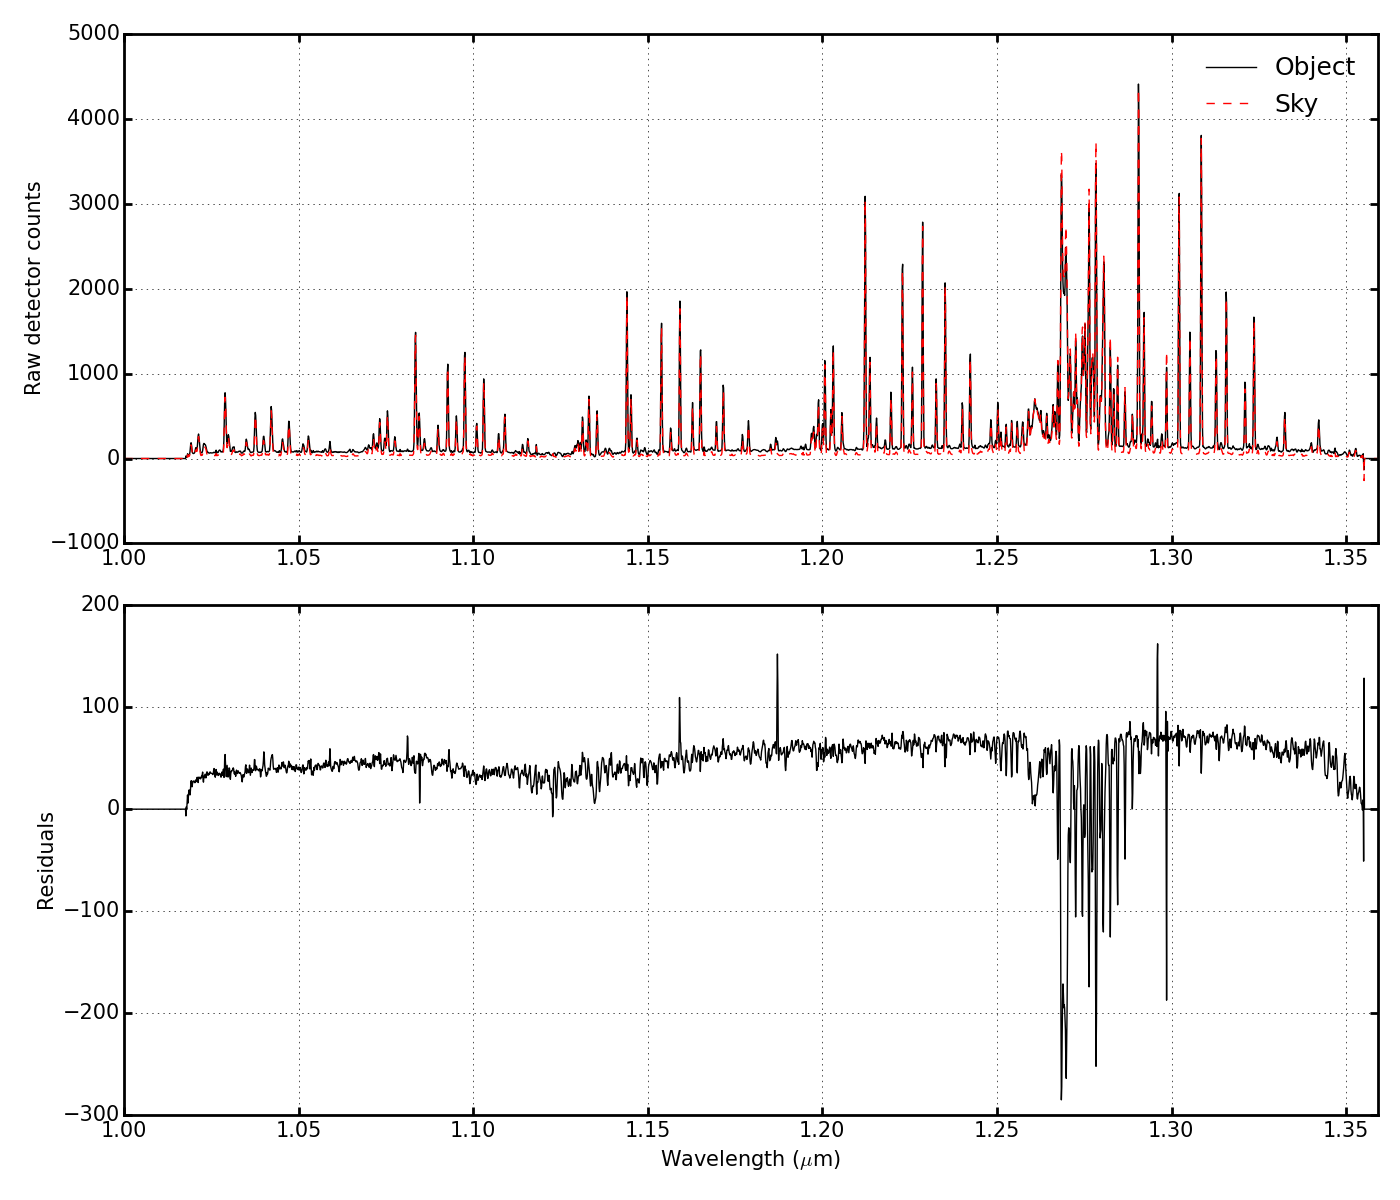
\includegraphics[width=0.85\textwidth]{kmos/NGC55-19-skysub_basic}
 \caption[Example of the sky subtraction procedure]{An example of the sky subtraction procedure. The top panel shows an object spectrum in black and an associated sky spectrum overlaid in red.
 The bottom panel shows the sky subtracted spectrum by simply subtracting the two spectra in the top panel.
 Note the difference in scale between the two panels illustrating that the signal from the sky is significantly larger than that from the object.
 \label{fig:skysub}}
\end{figure}

The second correction accounts for the absorption and re-emission of light from the science target by molecules within the Earth's atmosphere.
As the sophistication of this step is highly dependent upon the science case of the observations, for the general user this is implemented in a simplistic manner.
Typically, to perform this correction one observes an additional target of known spectral appearance: a telluric standard star.
This star is observed in each of the 24 KMOS IFUs in turn (or three IFUs depending upon the quality of the correction required) and the frames are calibrated using the same process as the science observations.

A spectrum is extracted from each IFU which is then divided by a model of the transmission of the atmosphere, the stellar features are then modelled with a simple Lorentzian function and removed.
This leaves a continuum spectrum of the star where the main features have been removed.
At this point the transmission model is then multiplied back into the spectrum and the shape of the spectrum is corrected with a blackbody spectrum with the effective temperature of the star.
Theoretically, these steps create a spectrum which contains only the light from the absorption of the Earth's atmosphere: the telluric spectrum.
The final target spectrum from an individual IFU is then divided by the telluric spectrum.

% subsection calibration (end)
% section data (end)

\section{Conclusions} % (fold)
\label{sec:conclusions}

In this chapter I have detailed the principles of spectroscopy and have outlined some of the key spectroscopic tools used to undertake astrophysical measurements, focussing on the diffraction grating and its uses in astronomy.
I have described IFS in detail and outlined some of the innovations which make this novel method possible.
I focus on using an advanced image slicer to perform IFS and outline why this method is superior to other approaches.
This leads onto a description of the instrument which is used for the observations in this thesis: KMOS.
In this section I detail some of the key features which make this instrument unique and highlight that KMOS has been applied to a range of science cases.
Finally, I describe the data products from KMOS and detail the process of calibration of the raw data.

% section conclusions (end)
% %%%%%%%%%%%%%%%%%%%%%%%%%
% Set up to be stand alone document
% All declerations in the header to be removed when added into thesis
%%%%%%%%%%%%%%%%%%%%%%%%%
% \documentclass[12pt]{article}

% \usepackage{booktabs} % booktabs provides professional formatting commands for tables
% \usepackage{amsmath} % amsmath provides extra maths symbols
% \usepackage{textcomp} % textcomp provides extra text symbols (like a degrees celsius symbol)
% \usepackage{../customisations}
% \usepackage{natbib}

% \title{$J$-band Sythentic Spectral Fitting}
% \date{\today}

% \begin{document}
% \maketitle
%%%%%%%%%%%%%%%%%%%%%%%%%
% To be included when added into thesis
\chapter{J-band Sythentic Spectral Fitting}
\label{ch:janal}

\section{Opening Remarks} % (fold)
\label{sec:opening}

In this chapter I describe in detail the process by which I implement an analysis
routine to fit synthetic spectra to observed data with the aim of estimating stellar parameters.
This analysis builds on existing methods while providing a fresh approach to various aspects of the routine.
I have developed this implementation in the public domain and the source code for this project is made publicly available
via an online repository.\footnotemark

\footnotetext{Souce code available from: https://github.com/lrpatrick/rsg-janal
although the interested reader should be aware that these routines are, at the time of writing, in development mode
in the sense that they are highly specialised to one machine and (particularly) one set of model grids}

In this chapter I first outline the principles of model atmospheres~\ref{sub:model_atmospheres}.
Where I discus the physics which is included in these models, some of their strengths and their limitations.
I then focus the discussion on the grid of synthetic stellar spectra which forms the base of this analysis routine in~\ref{sub:model_grid}.
In~\ref{sub:continuum_fitting} I detail the procedure of matching the continuum level of the observations with that of the models,
which leads on to~\ref{sub:best_fit_parameters} where the method by which the best fit parameters are selected is described.

Having described the analysis routine thoroughly I then test this routine and compare the results of this method to different implementations in~\ref{sub:compare}.
Finally, I conclude the chapter in~\ref{sub:conclusions}.

% section opening (end)
\section{Introduction to Stellar Model Atmospheres} % (fold)
\label{sub:model_atmospheres}

A stellar atmosphere is defined as the outer layers within a star which emitt radiation.
Therefore, by definition, the photons which we observe from a star have originated in the atmosphere.
Photons which have originated from deeper layers within the star have been absorbed and re-emitted by particles within the stellar atmosphere.
Stellar atmospheres are therefore vitally important in observational studies of stars, even though the fraction of the total mass of the star contained within the atmosphere is tiny ($\sim$~10$^{-10}$).
A nice analogy for visualising this layer and its thickness comes from the preface of~\cite{1989isa2.book.....B}, where these authors compared the skin of an apple to a hypothetical star which has been shrunk to the same scale and note that the skin of the apple is far thicker than the stellar atmosphere.


Even though stellar atmospheres contain a tiny fraction of the total stellar mass, these layers can have an enormous impact on the evolution of a star via stellar winds.
For example, in evolved massive stars, winds arising from the atmosphere can strip off the outer layers of the star to leave an exposed hydrogen and helium dominated core or push the star in a completed different evolutionary direction to become a RSG (see Chapter~\ref{ch:intro}).
In addition to having an impact on the evolution of the star, winds also help distribute material throughout their host galaxy and feed subsequent generations of star formation~\citep[e.g.][]{2011MNRAS.417..950H,2012MNRAS.421.3522H} thereby not only affecting the evolution of the star which the wind is produced, but by acting as part of a larger stellar population, affecting the evolution of their host galaxy.

By modelling stellar atmospheres, one can estimate fundamental stellar parameters by a comparison with observations.
The background theory and underlying physical assumptions of these models is the subject of the current section.
This is important to detail as without this background it is impossible to asses the effectiveness of the models and their limitations.

Two of the most fundamental equations which govern the properties of stellar atmospheres are,

\begin{equation}
    g = \frac{GM}{R^2},\label{eq:grav}
\end{equation}

\noindent and,

\begin{equation}
    T_{\rm eff} = \frac{F}{\sigma_{SB}} = \left(\frac{L}{4\pi \sigma_{SB}R^2}\right)^\frac{1}{4},\label{eq:Teff}
\end{equation}

\noindent where $g$ is the acceleration due to gravity, $M$ is the total mass of the star of radius $R$, $T_{\rm eff}$ is the effective temperature of the star, $F$ is the total flux per unit area, $L$ is the total luminosity of the star, $\sigma_{SB}$ is the Stefan-Boltzmann constant,  and $G$ is Newton's gravitational constant.

These equations define some fundamental observational properties of the model stellar atmospheres, using fundamental parameters of the models.
Equation~\ref{eq:grav} is defined by the density stratification of the model and equation~\ref{eq:Teff} is defined through the total flux emitted from the model.

In the following sections I detail three of the principle assumptions which are used to create a ``classical'' one dimensional stellar model atmosphere.
These assumptions underpin some of the most widely used model atmospheres.


\subsection{Hydrostatic Equilibrium} % (fold)
\label{sub:hydrostatic_equilibrium}

Any model of a star consists of a balance bewteen gravity and pressure in a gaseous material (or plasma considering the typical temperatures and densities within a star).
If a model is assumed to be static (i.e. not varying with time) the equation of hydrostatic equilibrium can be derived by considering the balance between the forces acting upon a small element of stellar material,

\begin{equation}
    \frac{dP(r)}{dr} = -\frac{\rho GM(r)}{r^2},\label{eq:hydro}
\end{equation}

\noindent where $P$ is the total pressure exerted within a radius $r$, $M$ is the total mass within a radius $r$, $\rho$ is the matter density~\citep[see Chapter 9 of ][for a simple derivation of this equation]{1989isa2.book.....B}.
As stated above, the mass contained within the atmosphere of a star is a negliable fraction of the total mass, therefore $M(r) = M_{tot}$ when considering this equation in the outer layers of the star.

The force exerted by pressure acting on an element of stellar material ($dP/dr$) can be considered as the sum of the forces acting upon it from gas pressure ($P_{g}$), radiation pressure ($P_{rad}$) and turbulent pressure ($P_{turb}$),

\begin{equation}
    \frac{dP_{tot}}{dr} = \frac{dP_{g}}{dr} + \frac{dP_{rad}}{dr} + \frac{dP_{turb}}{dr}.\label{eq:pressure}
\end{equation}

Equation~\ref{eq:pressure} illustrates that even though we have assumed the model is static, small scale turbulent motions must still be taken into account to accurately model stellar atmospheres.


% subsection hydrostatic_equilibrium (end)

\subsection{Mixing Length Convection} % (fold)
\label{sub:mlt}

Mixing length theory describes how convection is treated within the stellar atmosphere.
Typically, within a star, radiation is the main source of energy transport as the coefficient of diffusion is far smaller for particles (conduction) than for photons (radiation).
Only in degenerate cores does energy transport via conduction become important.

Convection is a very efficient form of energy transport where a macroscopic element of higher temperature rises an average distance into a region of lower temperature where it dissipates the excess energy being carried and mixes.
However, in order for convection to be effective, a driving mechanism must be established.
The atmosphere is unstable to convection if the Schwarzschild certerion is met,

\begin{equation}
    \nabla_{rad} > \nabla_{ad}
\end{equation}

\noindent where $\nabla_{rad} = (d~{\rm ln}\,T/d~{\rm ln}\,P)_{rad}$ is the radiative temperature gradient and $\nabla_{ad}$ is the adiabatic temperature gradient.
The driving mechamism for convection is usually a large temperature gradient within a particularly part of the star.
This can occur at various stages within the lifetime of a star, for example, most main sequence stars have a convective core which is a result of the temperature sensitivity of the CNO cycle which establishes a steep temperature profile.

The theory of convection is very difficult to to treat thoroughly.
The ``simple'' theory of mixing length convection~\cite{1958ZA.....46..108B,1965ApJ...142..841H} is widely used to implement convection within stellar atmospheres which assumes that the shapes and sizes of the elements which transport energy is fixed and that, on average, an element rises a characteristic length ($l_m$) before it dissipates energy.

If the Schwarzschild criterio is satisfied, the total flux ($F$) for a star is given by,

\begin{equation}
    F(r) = F_{conv} + F_{rad} = \sigma T_{eff}^4,\label{eq:flux}
\end{equation}

\noindent where $F_{conv}$ and $F_{rad}$ are the convective and radiative flux respectively.
An expression for the convective flux can be obtained by considering the excess energy dissipated by a rising element moving a distance
($\Delta r = l_m/2$) with an average velocity ($v_{conv}$).
The convective flux can therefore be expressed as,

\begin{equation}
    F_{conv} = \rho C_pv_{conv}\Delta T
\end{equation}

\noindent where $C_p$ is the specific heat at constant pressure and $\Delta T$ is the temperature difference between the element and surroundings, which can be expressed in terms of the different in temperature gradients.
Here the pressure scale height can be introduced using the assumption of hydrostatic equilibrium $H_p = dr / d{\rm ln} P = p/\rho g$ and an expression for the convective velocity can be estimated by assuming that half the work done by bouyancy is converted into kinetic energy,

\begin{equation}
    \frac{1}{2}\langle w\rangle \approx \frac{1}{2}\rho v_{conv}^2.
\end{equation}

The parameter $\alpha = l_m/H_p$ is introduced which typically takes the value $\alpha = 1.5--2.0$.
As a side note, in stellar evolutionary models, the value of $\alpha$ used can have a significant effect on the temperature of the models at the end of the RSG phase of evolution.


% subsection mlt (end)

\subsection{Local Thermodynamic Equilibrium} % (fold)
\label{sub:local_thermodynamic_equilibrium}

The assumption of thermodynamic equilibrium is where the temperature and density of a material can be considered constant (i.e. there are no net flows of energy).
Which is equivalent to assuming that the emitting source is a perfect black body.
Local thermodynamic equilibrium (LTE) is an approximation whereby the {\it local} properties of material can be assumed to be in thermodynamic equilibrium.
Stellar atmospheres can be approxmiated to be in LTE as their densities are sufficiently high that and density gradients are sufficiently low that their local properties are closely related to thermal equilibrium.

The three fundamental equations which can be defined assuming LTE are:

\begin{enumerate}
    \item The Boltzmann equation,
    \begin{equation}
        \frac{n_i}{N_I} = \frac{g_i}{U_I}e^{-E_i/kT},
    \end{equation}
    \item The Saha equation,
    \begin{equation}
        \frac{N_I}{N_{I+1}} = n_e\frac{U_I}{U_{I+1}}\left(\frac{h^2}{2\pi m_ekT}\right)^\frac{3}{2} e^{\chi/kT},
    \end{equation}
    \item The Maxwellian distribution of particles,
    \begin{equation}
        f(v)dv = \left(\frac{m}{2\pi kT}\right)^\frac{3}{2} \exp\left(\frac{-mv^2}{2kT}\right)4\pi v^2dv,
    \end{equation}
\end{enumerate}

\noindent where $n_i$, $g_i$ and $E_i$ are the population, statistical weight and energy of level $i$ respectively,
$N_I$, $U_I$ and $\chi_I$ are the total number density, partition function and ionisation potential of ionisation state $I$ (to which $i$ belongs),
$m$ is the mass of the particle, $v$ is the velocity of the particle, $T$ is the temperature of the particle and $k$ is the Boltzmann constant.

% These three equations describe the


% In addition the radiation source function (in the MARCS models -- not always the case) is assumed be be

% \begin{equation}
%     S_\lambda = \frac{\kappa_\lambda}{\kappa_\lambda + \sigma\lambda}B_\lambda(T) + \frac{\sigma_\lambda}{\kappa_\lambda + \sigma\lambda}J_\lambda
% \end{equation}

% More generally, in thermodynamic equilibrium $S_\lambda = B_\lambda$.
% In LTE

% subsection local_thermodynamic_equilibrium (end)

\subsection{Analysis of Assumptions and Summary} % (fold)
\label{sub:assumptions_summary}

The assumptions listed above allow one to obtain to create a ``standard'' stellar model atmosphere.
The assumptions listed above are known to be simplifications of the true picutre witih a stellar atmosphere.
For example, the assumption of LTE definitely breaks down in the atmospheres of stars as they are observed, and by definition emitt radiation.
However, using the above assumptions one can build a consistent model that, in general, agrees reasonably well with observations.

The treatment of convection is knowingly a large simplification as the shape and size assumed for the convective elements is constant whereas in reality the shapes of these elements could be described as funnel-like.
Full two- and three-dimensional hydrodynamical simulations are required to asses the assumption of mixing length convection which generally show that convective fluxes are smaller than those in more sophisticated prescriptions
\citep{2012sse..book.....K}.

The assumption of LTE typically holds in dense low levels of a star, however, in the atmosphere, where radiation is emitted, this is known to be a poor approximation.
This is particularly true in evolved stars where departures from LTE are expected owing to the low densities and surface gravities of their atmospheres.

Full non-LTE stellar model atmospheres are expensive to produce and as of yet, there exists no homogenous grid of model atmospheres which include these effects.
As a first step, one can use a homogeneous set of model grids computed in LTE and select particular elements with which to compute non-LTE deviations.
This is far less time expensive and produces reliable results over a large range of stellar parameters.


% subsection analysis_of_assumptions_and_summary (end)

% section model_atmospheres (end)

\section{Measuring Stellar Parameters with Synthetic Spectra} % (fold)
\label{sub:model_grid}

\begin{itemize}
    \item What are Synthetic Spectra?
    \item Why are they useful?
    \item Background to the J-band method
\end{itemize}

The spectra cover the $J$-band, specifically the $1.16-1.22\mu$m region, where there are various prominent spectral features.
These spectral features, arising from elemental absorption, are compared in the observed and model spectra,
where the $\chi^{2}$-statistic is calculated to asses the goodness of fit for each model.
The stellar parameters which are fit for in this analysis are global metallicity ($log (Z/Z_{\odot})$~=~[Z]), effective temperature (T$_{\rm eff}$), microturblence ($\xi$) and surface gravity ($log\,g$).
% In addition to these parameters, in the future I also hope to further develop this implementation to include the $\alpha$-to-iron ratio as a free parameter.
The observed spectra are fit with models from a set of MARCS model atmospheres
\citep{2008A&A...486..951G}.

The wavelength range, over which to perform this analysis,
is chosen based on the spectral appearance of the region.
Typically, in the spectra of cool stars, dense molecular absorption fetuares dominate the spectrum which require high-resolution spectroscopy to distinguish individual features and estimate stellar parameters in the $J$-band~\citep{Cunha07, Davies09a, Davies09b}.
However, in this small wavelength range the absorption is dominated by well separaeted elemental absorption features from iron, magnesium, silicon and titanium.
Therefore, the spectral resolution required in order to derive stellar paramters is significantly reduced.
This means that this analyis can be preformed with a relatively small amount of telescope time using multi-object spectrographs like the $K$-band multi-object spectrograph (KMOS)
or the multi-object spectrometer for infra-red exploration (MOSFIRE) and is therefore feasible for studies of red supergiant stars (RSGs) in external galaxies.

In addition to this, given the cool temperature of the outer layers of RSGs,
the peak brightness of a typical RSG is $\sim1.1\mu$m.
Combining this with the fact that dust attenuation is significantly lower in the near-IR, compared to the optical regime, RSGs are ideal candidates to be studied at large distances.

Previous implemenations of this analysis include that of
\cite{2010MNRAS.407.1203D} and Gazak (2014).
This implemenation includes aspects of both of these previous implementations and could be described as a hybrid of the two.
Eventually this analysis routine will be made publicly available will should encourage the community to engage with these routines.



The synthetic spectra used in this analysis is based on model atmospheres computed from the
MARCS model atmospheres project~\citep{2008A&A...486..951G}.
These model atmospheres are one-dimensional models (i.e. spherically symmetric)
computed within local thermodynamic equilibrium (LTE).
% where standard mixing-length theory is assumed.
The MARCS models are particularly general and widely applicable to many different types of stars and as such are well used and tested.
However, for the atmospheres of RSGs the assumptions which go into these models are known to break down
\citep{2002AN....323..213F,2010ASPC..425..124P},
therefore, in order to accurately analyse the spectra of RSGs additional corrections must be applied.

The MARCS model atmospheres used for this analysis are computed with a mass of $15M_{\odot}$.
The typical mass range of a RSG is $8~\textendash~40M_{\odot}$, however,
using this mass is applicable owing to the fact that altering the mass of these models affects only the extension
(or geometrical thickness) of the models which does not change for red giants or supergiants
\citep{2010MNRAS.407.1203D}.

To improve the accuracy of the model atmospheres,
non-LTE calculations have been performed for all elements which give rise to the diagnostic features within the wavelength range studied
\citep{2012ApJ...751..156B,2013ApJ...764..115B,2014arXiv1412.6527B}.
% and therefore all of the lines used as diagnostic lines have non-LTE calculations preformed.
Line profiles and non-LTE corrections are calculated using an updated version of the SIU code
\citep{1999PhDT.........3R,2012ApJ...751..156B}.

The parameters of the resulting grid of model spectra are detailed in
Table~\ref{tb:grid}.
The model spectra are at $R~=~10\,000$,
which is chosen to be significantly higher than the typical resolution of the observed spectra
(i.e. $R~\sim~3000$).
The sensitivity of each diagnostic line for a given free parameter is illustrated in figures~\ref{fig:mod-z} through~\ref{fig:mod-micro}.

From an analysis of figures~\ref{fig:mod-z} and~\ref{fig:mod-g} it can be seen that the effect of increasing the metallicity of the models is similar to that of decreasing the surface gravity.
It is therefore expected that a degeneracy exists between metallicity and surface gravity.
This degeneracy is explored further in~\ref{sub:best_fit_parameters}.

The effect of varying the temperature of the models changes the relative strengths of the lines of different spectral species.
For example, see the left panel in Figure~\ref{fig:mod-t} where the ratio of the iron
($\lambda\,1.188285$) to titanium ($\lambda\,1.189289$) lines is strongly affected by varying the temperature of the models.
Also note that each species does not respond linearly to temperature.
This can be seen by a comparison between the strength of the iron line
($\lambda\,1.197305$) in the right hand panel of figure~\ref{fig:mod-t} to that of the silicon lines
($\lambda\lambda\,1.198419, 1.199157$) in the same panel.
This is clearly distinguishable from all the effects of all other parameters.


Increasing the microturblence has the effect of increasing the equivalent widths
of the strongest lines preferentially as well as affecting the relative strengths of the lines arising from the same spectral species.
Therefore, features arising from the same element will be most sensitive to this
parameter.
This is illustrated by a comparison between the two strong iron lines
($\lambda\lambda\,1.188285, 1.197305$) in the left and
right panel of Figure~\ref{fig:mod-micro}.
We see that at $\xi~=~1.0$ the iron line in the left panel is strongest,
whereas at $\xi~=~5.0$, the iron line in the right panel is the stronger of the two.


\begin{table}
\caption{Model grid parameter space\label{tb:grid}}
\scriptsize
\begin{center}
\begin{tabular}{lccc}
 \hline
 \hline
Parameter & Abbreviation & Range & Increment \\
 \hline
Global Metallicitiy & $[Z]$ & $+1.0~\textendash~-1.0$ & 0.1\,$dex$ \\
Effective Temperature & $T_{\rm eff}$ & $3400 ~ \textendash~4400$ & 100\,$K$ \\
Log gravity & $log g$ & $+1.0~ \textendash~-1.0$ & 0.25\,$dex$ \\
Microturblence & $\xi$ & $1.0~ \textendash~5.0$ & 0.2\,$km\,s^{-1}$ \\
 \hline
\end{tabular}
\end{center}
\end{table}


\begin{figure}
 \centering
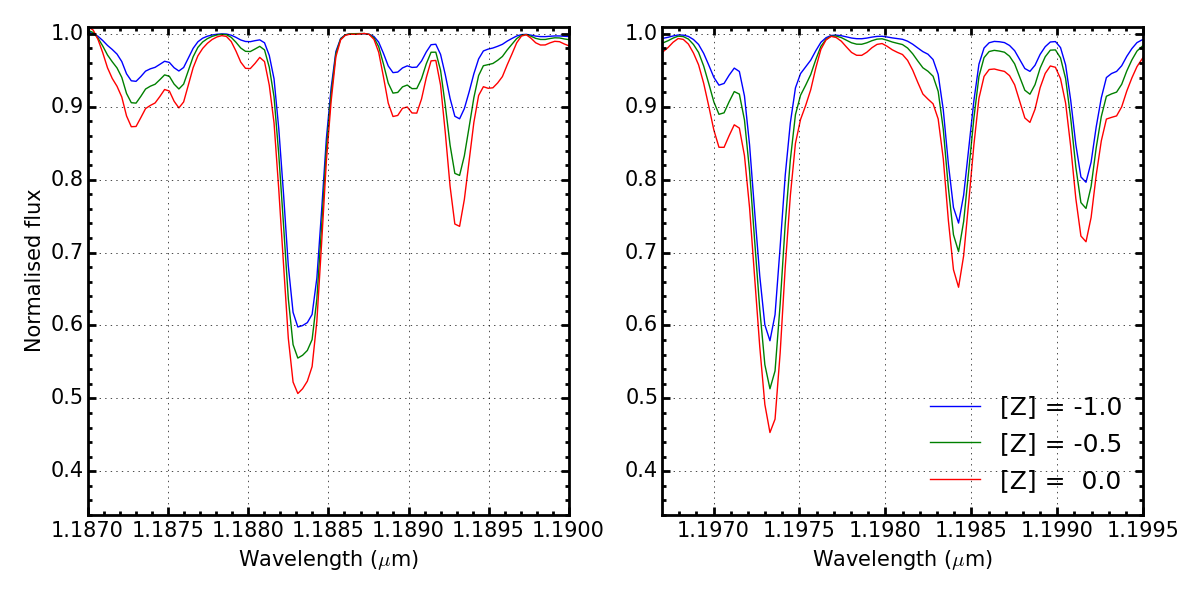
\includegraphics[width=0.65\textwidth]{JAnal/varyZv2}
\caption{
Three models where only the metallicitiy is varied.
Five diagnostic lines are shown in two panels.
Left: Fe\,I $\lambda$1.188285 and Ti\,I $\lambda$ 1.189289.
Right: Fe\,I $\lambda$ and Si\,I $\lambda\lambda$ 1.198419, 1.199157.\label{fig:mod-z}
         }
\end{figure}

\begin{figure}
 \centering
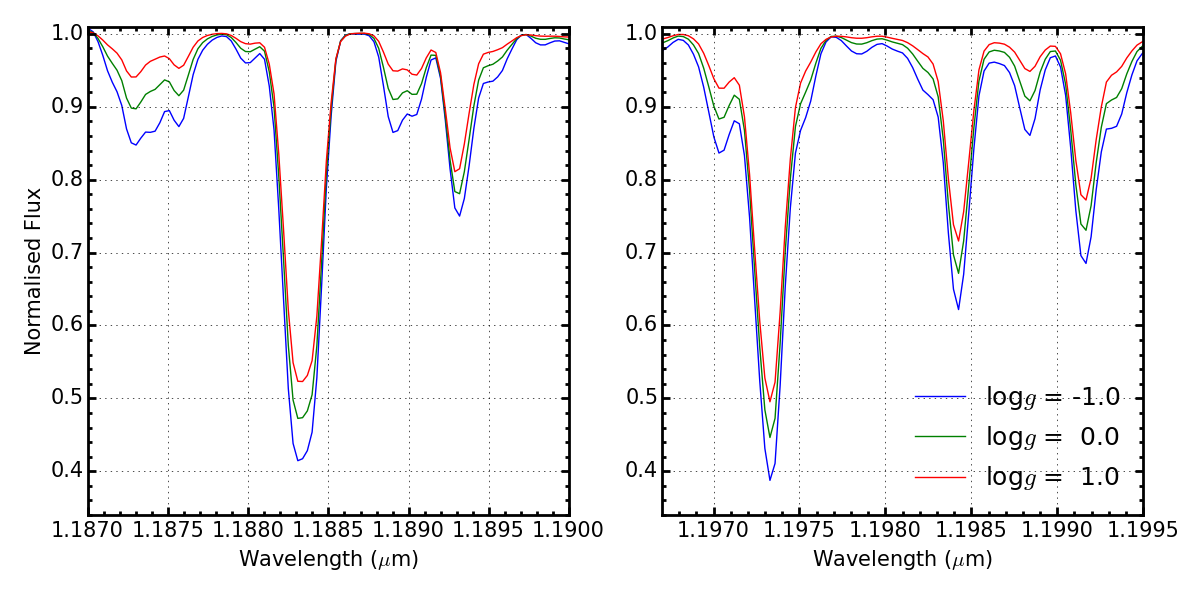
\includegraphics[width=0.65\textwidth]{JAnal/varygv2}
\caption{
As in Figure~\ref{fig:mod-z} where however surface gravity is varied.\label{fig:mod-g}
         }
\end{figure}

\begin{figure}
 \centering
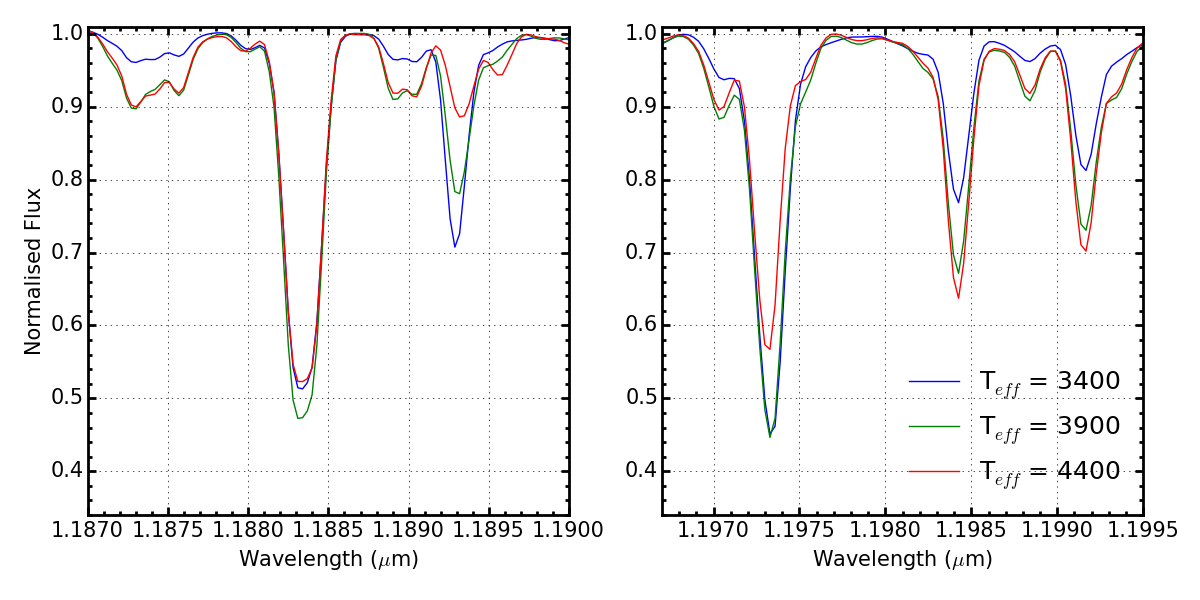
\includegraphics[width=0.65\textwidth]{JAnal/varyTv2}
\caption{
As in Figure~\ref{fig:mod-z} where however effective temperature is varied.\label{fig:mod-t}
         }
\end{figure}

\begin{figure}
 \centering
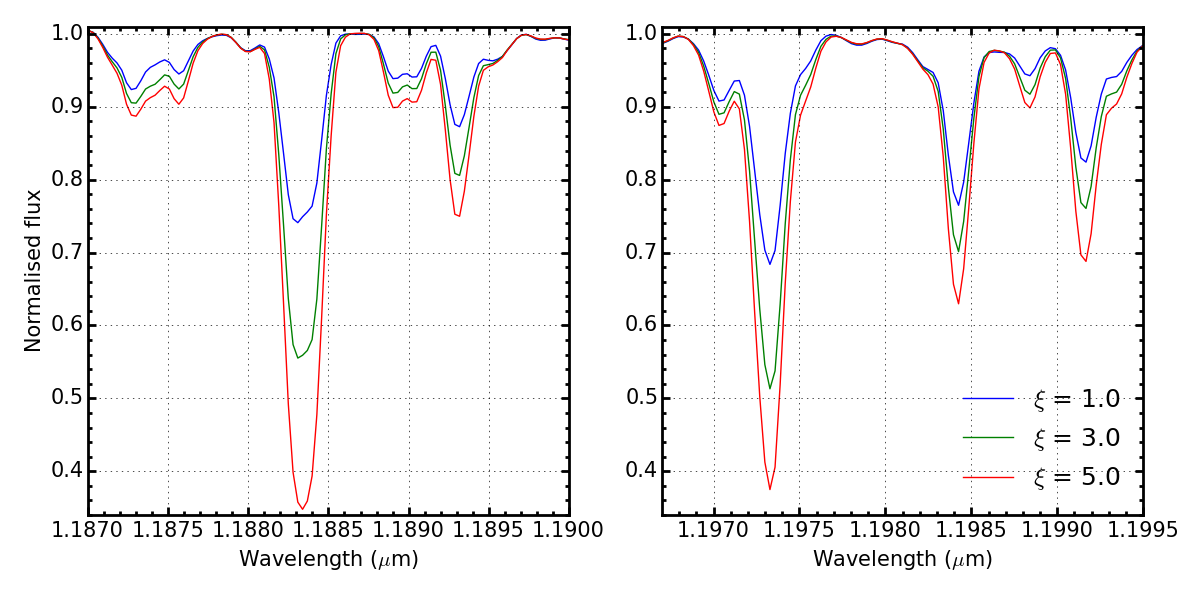
\includegraphics[width=0.65\textwidth]{JAnal/varymicrov2}
\caption{
As in Figure~\ref{fig:mod-z} where however microturblence is varied.\label{fig:mod-micro}
         }
\end{figure}

The current model grid is sufficient to explore the parameters for a typical RSG.
However, when using this technique at larger distances,
many different metallicity environments are encountered (e.g. the low metallicity environment ofI\,Zw\,18 with $Z=(1/32)Z_{\odot}$~\citep{1998ApJ...508..248V}).
In order to study these extremely low-metallicity systems,
the metallicity parameter space would need to be extended.
The $\alpha$-to-iron ratio of these stars is taken to be that of the solar value and is not left as a free parameter in the models.
This is applicable as young stars are known to have solar-like $\alpha$-to-iron ratios in different metallicity galaxies
~\citep[see tables 3 and 4 in][and references therein]{2015ApJ...806...21D}.

% \begin{itemize}
%     \item How are the grids generated?
%     \item What are the non-LTE corrections?
%     \item What do the current grids look like?
%     \item How could they be improved?
% \end{itemize}
% section model_grid (end)
\section{Continuum Fitting} % (fold)
\label{sub:continuum_fitting}

Accurately matching the continuum levels in the observed
spectrum provides a base with which to anchor the diagnostic lines of the models.
An incorrectly placed continuum level would bias the analysis and result in the
strength of the diagnostic lines being over or under estimated producing inaccurate stellar parameters.

% The continuum fitting procedure is important because determining the base of the
% diagnostic lines defines their overall strength which is used to distinguish
% between models.
There are many factors that effect the level of the continuum and continuum placement,
including the resolution of the observations as well as the stellar parameters themselves.
Therefore it is vital that when attempting to derive stellar parameters,
in crowded regions such as this, the continuum placement is performed
consistently and accurately.
Intrinsically, when studying RSGs at medium resolution - owing  to their cool atmospheres -
there are many instances of blended spectral features.
At this resolution the density of blended spectral features creates a pseudo-continuum which, in practice,
is never at the ture continnum level.
Figure~\ref{fig:mod-res} illustrates the varying continuum levels for models where the resolution is varied and
Figure~\ref{fig:mod-zcont} shows this affect when varying only the metallicity.
It can also be seen in figures~\ref{fig:mod-z}---\ref{fig:mod-micro} that each of the parameters affects the continuum in a subtly different manner.

\begin{figure}
 \centering
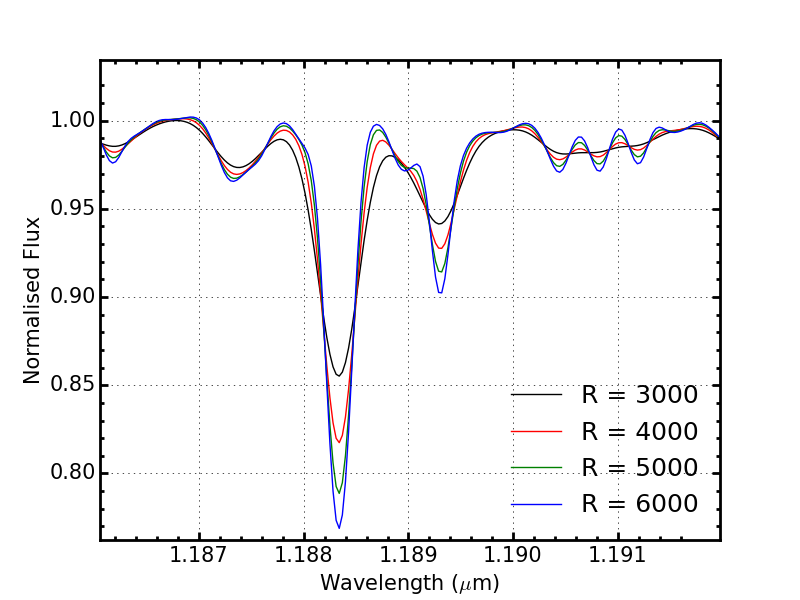
\includegraphics[width=0.65\textwidth]{JAnal/Resolution}
\caption{
One model degraded to four different resolution values.
This figure demonstrates the how the continuum level changes depending upon
the resolution of the spectrum.
We see at around 1.191$\mu$m at $R=3000$ the continuum level is perturbed by blended lines.\label{fig:mod-res}
         }
\end{figure}

\begin{figure}
 \centering
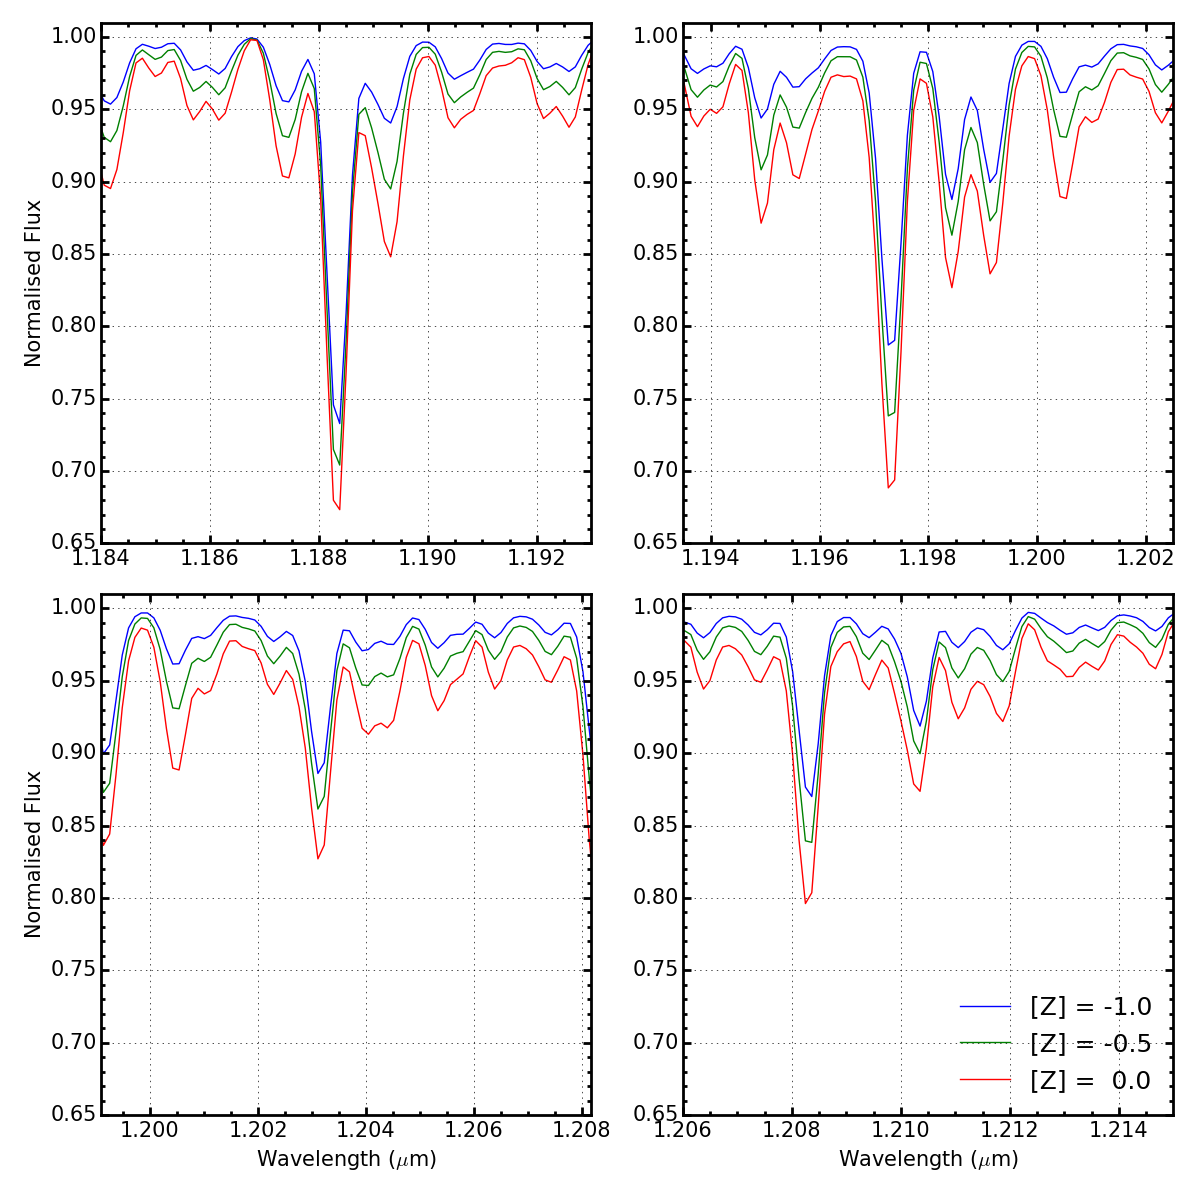
\includegraphics[width=0.65\textwidth]{JAnal/varyZ}
\caption{
Three models where only the metallicitiy is varied.
Each panel shows one or more diagnostic line.
Metallicity of the model intrinsically affects the continuum level of the spectrum,
such that at higher metallicities, there is greater departure from the true continuum level, which in the case of the models is 1.00.\label{fig:mod-zcont}
         }
\end{figure}


Given that it is impossible to know the true continuum level from any given observation,
the scaling applied must be consistent between the models and observations.
Scaling is required not only to match the levels of the continuum placement, but also to match the line strengths between the models and observations.
Providing the treatment of the models and observations are consistent, the fact that the true continuum is never attained is not significant
\citep{2014ApJ...788...58G}.
For the process of continuum matching to work effectively,
the observed and model spectra should be at the same resolution,
have a consistent wavelength calibration
and have identical spectral sampling.

In order to account for differences in the spectral sampling of the observed and model spectra,
each model spectrum is resampled onto the wavelength scale of the observations by means of a spline interpolation routine.
The model spectrum is then degraded to the resolution of the observations by a
convolution with a Gaussian filter where the width of the Gaussian is defined by the observed resolution ($FWHM~=~\sqrt{(\lambda/R)^{2} -(\lambda/R_{mod})^{2}}$ where $R$ is the resolution of the observed spectrum).
The resolution of the KMOS observations is estimated using the KMOS/esorex pipeline from arc lamp exposures at the appropriate rotator angle for the observations.
This is measured for each spectrograph and is assumed to be constant (to within $\pm 100$) across individual IFU's as well as across the detector.

% This is accounted for by degrading the sampling of the models to that of the observations by means of a linear interpolation.
% The sampling of the models are degraded to that of the observations by means of a cublic-spline interpolation.
To ensure the spectra are on the same wavelength scale, the observed specturm is cross-correlated with the model spectrum;
a shift is then applied to the observed spectrum in order to minimise the cross-correlation matrix.
This procedure is repeated until the shift between the observed and model spectra is less than $0.1\,pix$.
Over this small wavelength range, one would not expect significant variations in the spectral resolution of the observations to perturb the cross-correlation.

Once the spectra have been correctly matched they are now suitable to be compared over the wavelength range $1.165-1.215\mu$m.
To estimate the amount of scaling required first I define the continuum width ($cw$) as:

\begin{equation}
    cw~=~\frac{\lambda}{R}, %\times S,
\end{equation}
\noindent where $R$ is the resolution of the spectrum and
$\lambda$ is the wavelength at which the width is taken
(in principle this wavelength varies across the spectrum, however, given our spectral window is sufficiently small, I assume $\lambda~=~1.20\mu$m).
% and $S$ is a scale factor which takes the range $0.5 < S < 1.0$.
The continuum width is essentially the resolution element of the spectrum at a wavelength of
$\lambda~=~1.20\mu$m and defines the width in which we expect to find a combination of pixels from a spectral feature and the continuum.

% multiplied by the scale factor $S$.
% In Gazak et al. (2015) this scale factor is fixed at 0.5.
% The scale factor is introduced because ... ?

The model spectrum is divided into wavelength slices each of width $cw\mu$m and the maximum of each slice is taken.
Using this array of maxima any major feature is systematically removed by rejecting data points more than 3$\sigma$ from the mean of the distribution.
Figure~\ref{fig:cw} illustrates the width of these slices and how this technique  removes prominent spectral features.
In this figure blue points represent the boundaries between the slices of width $cw\mu$m and the maximum of each slice is shown in red.
 % using this technique systematically removes absorption features from the spectrum.
% Any remaining features in this maximum spectrum are removed by rejecting outliers which are more than 3$\sigma$ from the mean of the distribution.
% In figure~\ref{fig:cw} the $cw~max.$ points have been through this procedure.
% This can be seen by noting that the cores of the absorption lines no $cw max.$
% points present.

\begin{figure}
 \centering
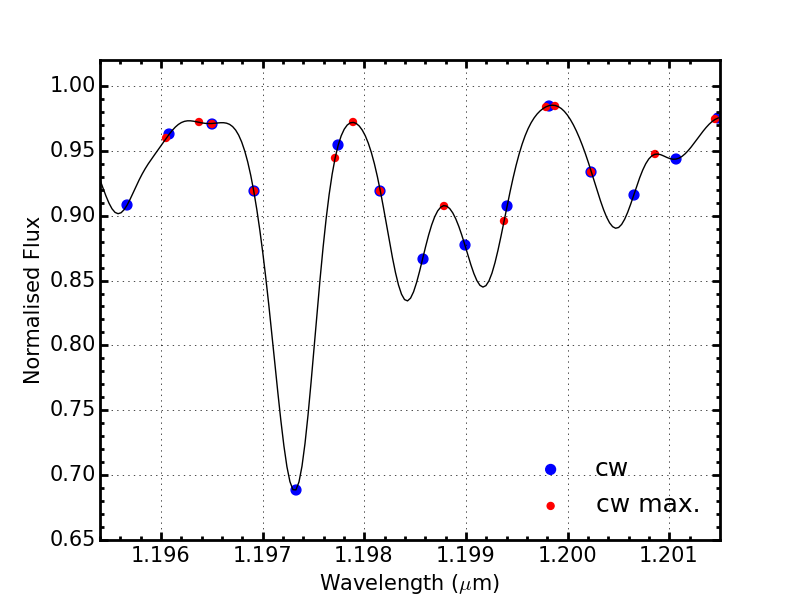
\includegraphics[width=0.65\textwidth]{JAnal/cw}
\caption[Illustration of continuum width slices and maxima]{
Illustration of the continuum width ($cw$) and slicing the model spectrum into regions of $cw\mu$m is able to remove structure in order to fit the continuum.
The solid black line shows an example of a model spectrum degraded to a resolution of 3000,
blue points show the boundaries between the slices and red points show the maximum of each slice.\label{fig:cw}
         }
\end{figure}


The remaining data points ($P_{cont}$) are used to derive an initial correction function
($cf_{1}$) by fitting a third-order polynomial to the ratio of the model to observed continuum points (red points in figure~\ref{fig:cw}), defined using the equation:
\begin{equation}
    cf_{1}~=~f(\frac{F_{mod}(P_{cont})}{F_{obs}(P_{cont})}),
\end{equation}

\noindent where $F_{mod}$ and $F_{obs}$ are the flux in the model and observed spectrum respectively.
The final correction function ($cf_{2}$), a refinement of $cf_{1}$,
is defined by removing any remaining outliers more than 3$\sigma$ from the mean of the correction function $cf_{1}$.
This method assumes that over the small wavelength range considered,
$cf_{1}$ does not vary significantly from the mean and as such, any significant deviation is considered originating from a spectral feature or noise.

The final correction function, $cf_{2}$,
is used to define the amount of scaling required for the model.
Figure~\ref{fig:cftaction} shows how the continuum fitting process works using a model spectrum as the observed spectrum (black) and a second model spectrum
(blue dashed) which is scaled to match the continuum level of the observed
(red dot-dashed).
It can be seen that the continuum placement of the example observed spectrum and that of the scaled model spectrum is well matched, even though the line strengths don't match well.

\begin{figure}
 \centering
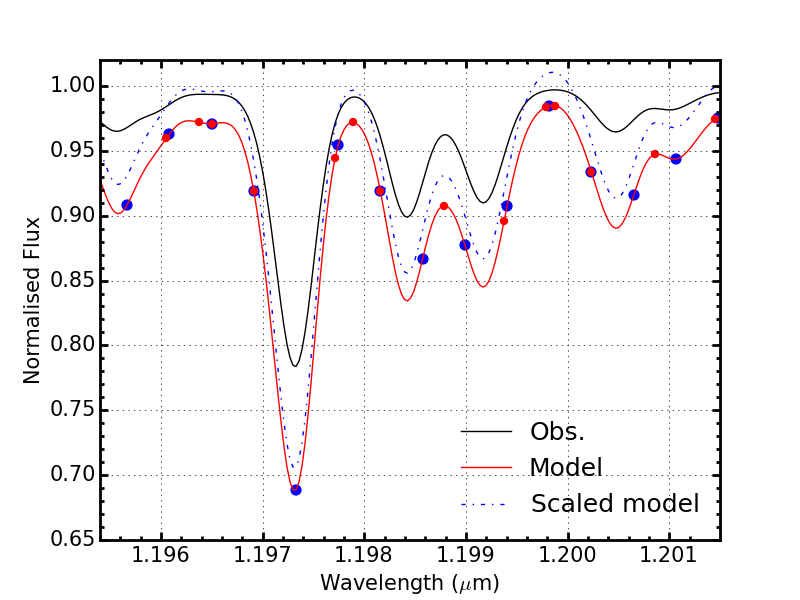
\includegraphics[width=0.65\textwidth]{JAnal/cftaction}
\caption[Example of continuum fitting]{
An example of how the continuum fitting procedure works using a model spectrum as
an example observed spectrum (black solid line)
and a separate model spectrum to match the level of the continuum.
The dashed blue spectrum denotes the model spectrum before any scaling has taken place.
The dot-dashed red spectrum denotes the model spectrum after the continuum fitting scaling has been applied.
The red and blue points the edges of the slices made and maxima of these regions respectively.
For these models, the true continuum level is at 1.00.\label{fig:cftaction}
         }
\end{figure}


% The green dashed line shows a third order polynomial fit to the ratio of the model spectrum to a simulated observed spectrum at only the red points ($~=~\frac{F_{mod}(cf_{1})}{F_{obs}(cf_{1})}$).

Alternative methods of continuum fitting are discussed in~\cite{2010MNRAS.407.1203D} and~\cite{2011A&A...527A..50E}.
These methods select pseduo-continuum pixels in the models based on ranking the model pixels and selecting a percentage of the pixels with the largest flux.
Providing the pixels from the model are selected in this manner and not those in the observations, this is a reliable method with which to derive the continuum level as demonstrated by~\cite{2015ApJ...806...21D}.
% \textbf{What advantage (if any) does the method applied here have over the one used in Davies et al. (2015 in prep.)?}

% section continuum_fitting (end)
\section{Best Fit Parameters} % (fold)
\label{sub:best_fit_parameters}

Best fit parameters are calculated using a chi-squared minimisation approach.
Each model is compared to the observed spectrum
and the chi-squared statistic is calculated using the equation,

\begin{equation}
    \chi^{2}~=~\frac{1}{N_{pix}}\sum\limits_{i}{\frac{(O_{i} - M_{i})^{2}}{\sigma^{2}}},
\end{equation}

where $N_{pix}$ is the number of pixels used and
$\sigma$ is determined by the S/N of the spectrum.
This statistic is calculated over each of the diagnostic lines and here $N_{pix}$ is the total number of pixels used to perform this calculation.
Table~\ref{tb:lines} details the diagnostic lines used in this analysis.
The amount of continuum included to compute the $\chi^{2}$-statistic is important to consider.
If this wavelength range is too small, the wings of the lines will be neglected,
which would discard vital information used to constrain the model parameters.
However, if too much of the pseudo-continuum is included, the parameters could be biased by noise features in the observations or by inaccuracies within the models.
For example,
~\cite{2014PhDT.........G} identify several spectral features present in the observed spectra which are missing in the model spectra.
The regions which are used in the calculation of the $\chi^{2}$-statistic are highlighted red in
figure~\ref{fig:lines}.
There are multiple cases where the diagnostic lines are sufficiently close together that, at R$\sim$3000,
the lines are not clearly separated.
In these instances, the most appropriate course of action is to define a region which encompasses all of the spectral features in question,
% the region where the $\chi^{2}$ is computed over all of the lines in question and to deal with the region as a whole,
as illustrated in Figure~\ref{fig:lines}.
This ensures that an individual pixel is not counted multiple times and provides a more applicable edge for which to compute the $\chi^{2}$-statistic.

\begin{figure}
 \centering
 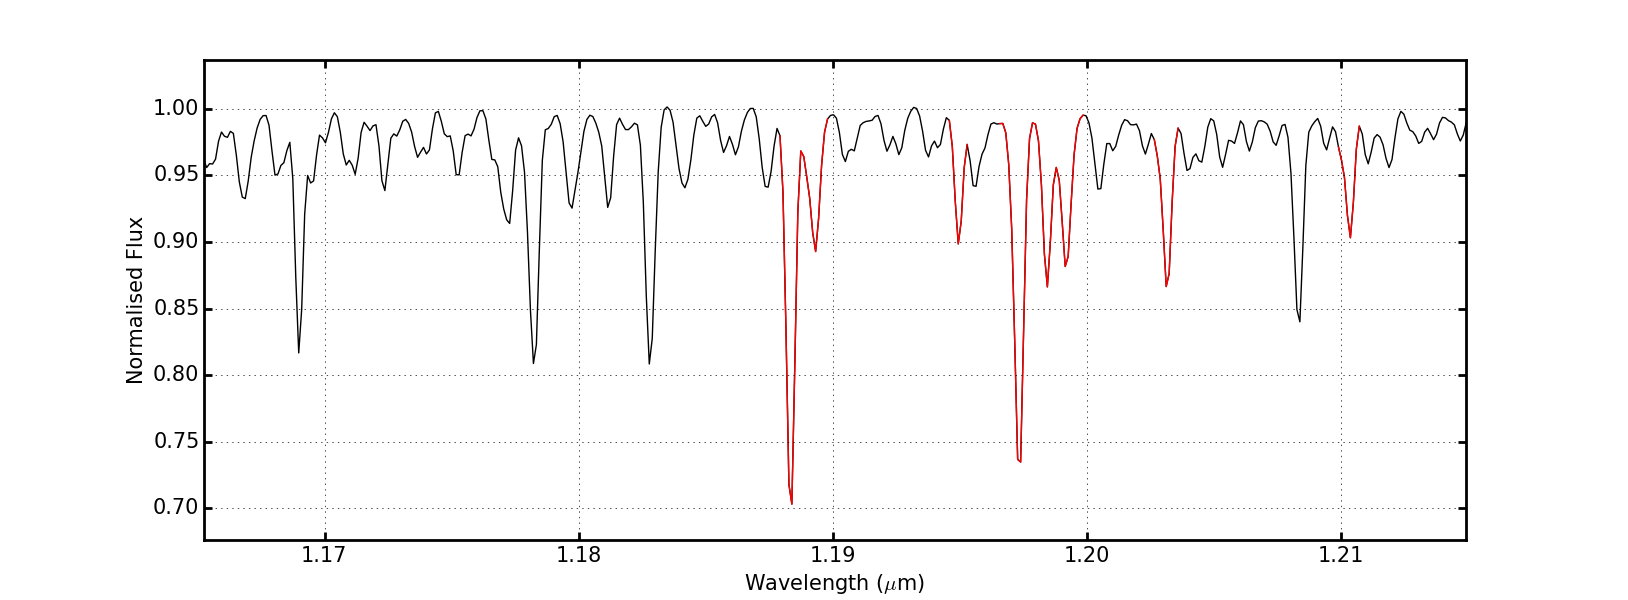
\includegraphics[width=0.65\textwidth]{JAnal/Diag-lines}
 \caption[Diagnostic lines]{
An example of a model spectrum, degraded and resampled to that of a typical observed spectrum (in this case NGC6822-RSG01), where the regions used to compute the $\chi^{2}$ calculation is highlighted in red.\label{fig:lines}
         }
\end{figure}

\begin{table}
\caption[Diagnostic lines]{Diagnostic lines\label{tb:lines}}
\scriptsize
\begin{center}
\begin{tabular}{cc}
 \hline
 \hline
Species & Line Centre \\
 \hline
Fe\,I & 1.188285 \\
Fe\,I & 1.197305 \\
Si\,I & 1.198419 \\
Si\,I & 1.199157 \\
Si\,I & 1.203151 \\
Si\,I & 1.210353 \\
Ti\,I & 1.189289 \\
Ti\,I & 1.194954 \\
Mg\,I & \\
Mg\,I & \\
 \hline
\end{tabular}
\end{center}
\end{table}

Each best fit parameter is estimated based on a weighted average,
where the weights are determined by the $\chi^{2}$ value of the model:

\begin{equation}
    w~=~exp(-\chi^{2}/2).
\end{equation}

The average is performed using the 100 models with the lowest $\chi^{2}$ value.
\begin{itemize}
    \item Why is 100 chosen?
    \item Doesn't this bias models at the edge of the grid? (e.g. figure~\ref{fig:test2})
    \item I need more on this in general!
\end{itemize}

Errors on the parameters are determined by defining
$\Delta\chi^{2}~=~\chi^{2}_{min} + 3$.
The standard deviation of the models parameters for all models which have a
$\chi^{2}$ value within this range define the errors.
For a purely Gaussin distribution the 1$\sigma$ deviation is $\Delta\chi^{2}~=~2.3$.
However, assuming one of the diagnostic lines is only fit to within 2$\sigma$ while the rest being fit to within 1$\sigma$, we obtain $(n_{l}~-~1)~\times~1^{2}~+~1~\times~2^{2}~=~n_{l}~+~3$
where $n_{l}$ is the number of lines used.

As mentioned previouslly (in~\ref{sub:model_grid}) and as demonstrated in
~\cite{2015ApJ...806...21D} there exists a degeneracy between the effect of decreasing the metallicity and increasing the surface gravity of the models.
To help break this degeneracy, I implement an additional gravity restraint.
This works by calcualting the luminosity of the observed star using near-IR photometry and the bolometric correction given in~\cite{Davies13b}.
Having calculated the luminosity, the relationship,
\begin{equation}
    \frac{g}{T^{4}_{\rm eff}}~\propto~\frac{M}{L},
\end{equation}
can be used to restrict the $log\,g$-T$_{\rm eff}$
parameter space using sensible limits for the mass of a RSG
($8~\leq~M/M_{\odot}~\leq~40$).
Where $M$ is the mass of the star,
$T_{\rm eff}$ is the effective temperature and $g$ is the surface gravity of the star.
These regions of parameter space are rejected from the analysis as unphyiscal.

To test the accuracy of the analysis routine, I begin with the most simple test I can imagine:
do I recover the parameters when using a model spectrum as input?
In every test performed in this fashion the model parameters are recovered within 1$\sigma$ across the full model grid.
To increase complexity, a small amount of noise is added to this model spectrum prior to the analysis.
Again, with all models tested (which span the full grid of model parameters) the input stellar parameters are derived to within the 1$\sigma$ errors.

The second test performed, which is a small step up in complexity, is to use a model spectrum as input, degraded to the resolution and sampling of a typical observation (in this case I use $R~=~3000$ with a sampling equal to that of the KMOS YJ grating at its natural sampling).
In addition, Gaussian noise is added to the input spectrum with the S/N~=~100
(characteristic of the poorest S/N typically observed).
The results of this test are illustrated in figure~\ref{fig:test2}.
From this figure it can be seen again that typically we see excellent agreement between the input parameters and the output parameters.
Note, all of these tests assume that the luminosity of the model is known
(idential to the assumption made when using this analysis on real data).

\begin{figure}
 \centering
 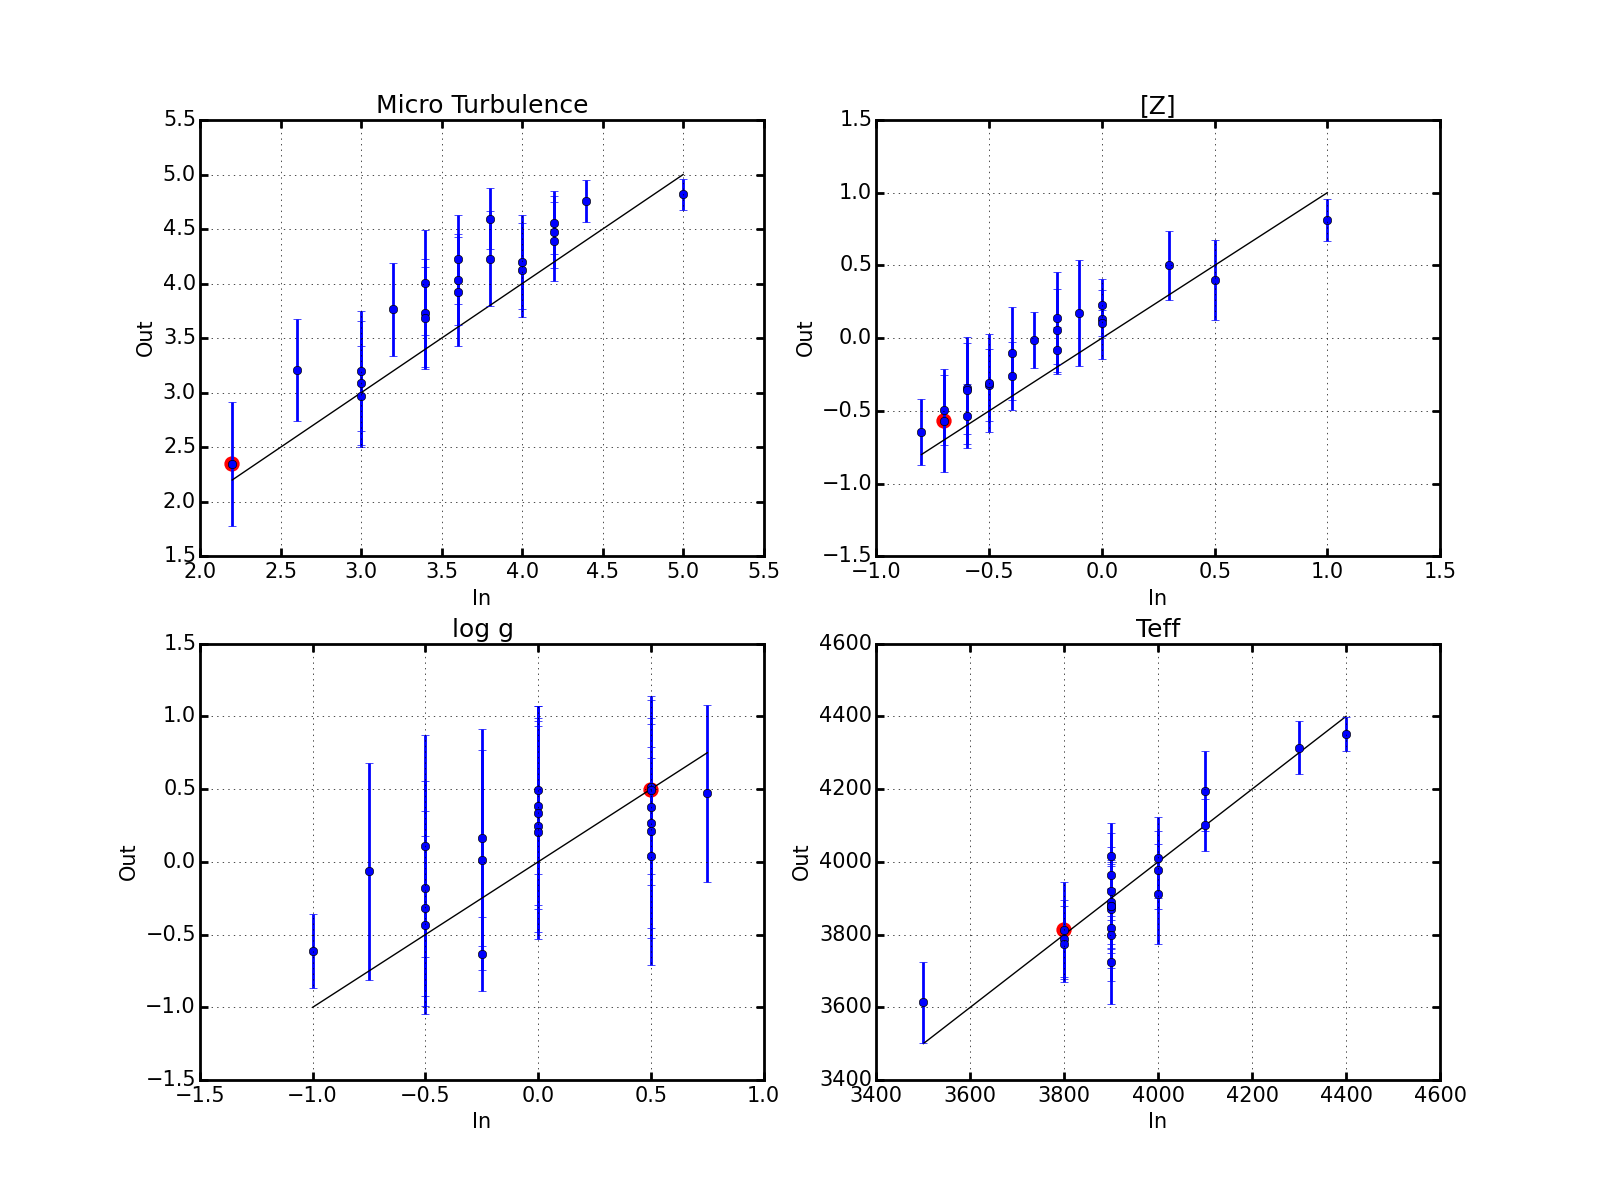
\includegraphics[width=0.65\textwidth]{JAnal/lineonly-test2v22}
 \caption[Test ]{
Results of the analysis routine using 21 fake RSG spectra as input.
The spectra span a wide range of stellar parameters and are degraded to $R~=~3000$ and resampled onto a typical sampling for the real data with random Gaussian noise added of S/N~=~100.
\label{fig:test2}
         }
\end{figure}

\section{Comparisons With Previous Implementations} % (fold)
\label{sub:compare}
To increase confidence in the accuracy and reliability of this implementation of the $J$-band synthetic spectral fitting methods,
where applicable, these routines have been compared to the results based on previous implementations of this analysis.

To date, there are currently two other published implementations using medium resolution $J$-band spectra of RSGs to derive stellar parameters,
that of~\cite[][DFK10]{2010MNRAS.407.1203D} and that of
\cite[][G14]{2014PhDT.........G}.
Both of these implementations are subtly different and use different assumptions to derive the stellar parameters.
They are both broadly based on the same techniques used in this analysis,
however, the main differences between the two methods are that DFK10 uses just the line strengths of the diagnostic lines to calculate the $\chi^{2}$ statistic,
while G14 uses the entire $1.165-1.215\,\mu$m region (with some exceptions).

In the current implementation, the diagnostic lines themselves are used to calculate the $\chi^{2}$ statistic.
This is preferred to the two aforementioned techniques for the following reasons:

1. The models used in the analysis are not perfect representations of RSG spectra.
The line list which builds these spectra are known to be incomplete and the effect of including these wavelength regions within the $\chi^{2}$ calculation could be to perturb the fit. G14 is very careful to exclude all known instances of missed lines within the models, however, this can not be assumed to be a complete consensus of missed lines.

2. Using the full line profile of the diagnostic lines provides information on the shape of the lines which using the line strength does not.

\subsection{DFK10} % (fold)
\label{sub:dfk10}
To date there have been several published articles using the DFK10 implementation
~\citep{2010MNRAS.407.1203D,2015ApJ...803...14P,2015ApJ...806...21D}.
The original implemetation was updated and tested rigourously on VLT-XSHOOTER spectra of RSGs in the Magellanic clouds in
~\cite{2015ApJ...806...21D} and in~\cite{2015ApJ...803...14P} this was applied to KMOS spectra in NGC\,6822.
In this section we compare the analysis routine detailed above with that of DFK10 on the set of 10 RSG KMOS spectra in NGC\,6822.
Figure~\ref{fig:n6822DFK} shows the comparison of the output parmaters of the stars in this sample for the two analysis routines.
This figure shows that the agreement between the two routines is acceptable for all stellar parameters.
The mean of each of the parmeters is calculated in Table~\ref{tb:DFK10} and is shown to agree within the errors.

\begin{figure}
 \centering
 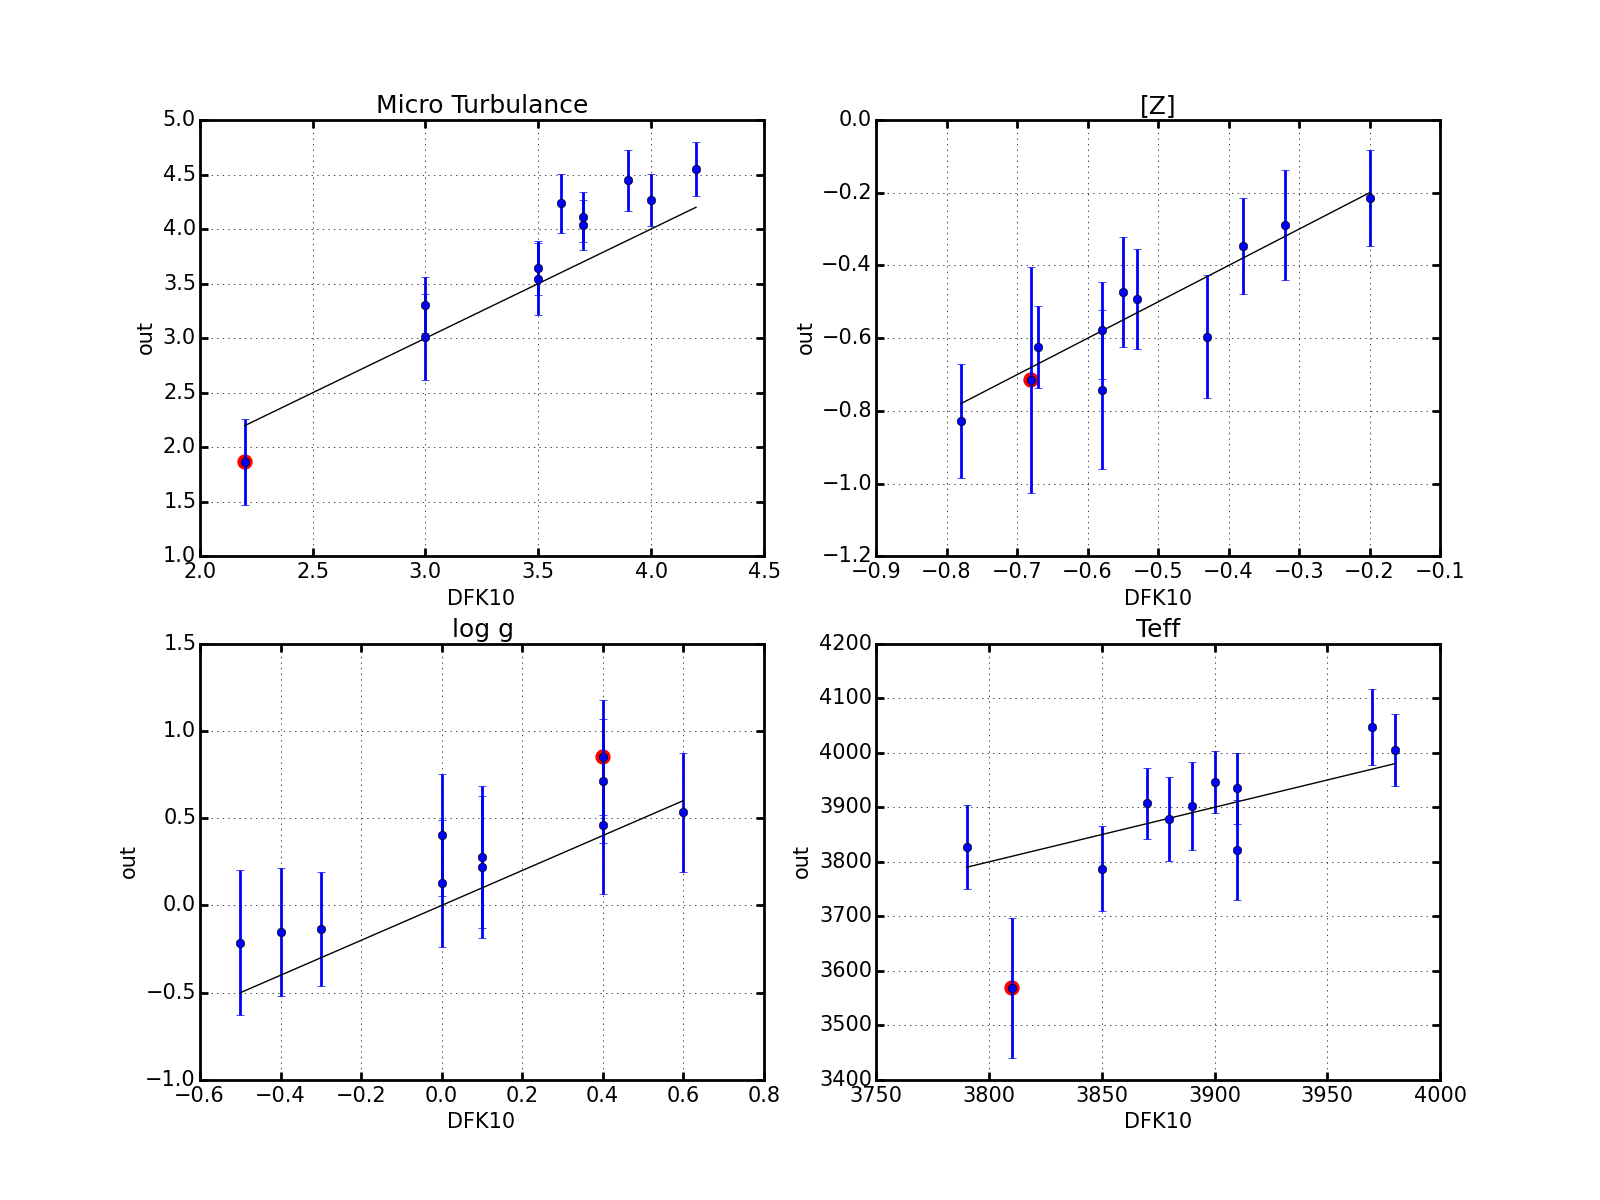
\includegraphics[width=0.65\textwidth]{JAnal/compare-DFK10}
 \caption[NGC\,6822 DFK10]{
A comparison between the parameters derived for 11 RSGs in NGC\,6822.
DFK10 results are those published in~\cite{2015ApJ...803...14P}.
\textbf{Note: I haven't commented on the offset between the parameters as I'm assuming I will be able to crack this soon!}\label{fig:n6822DFK}
         }
\end{figure}

\begin{table}
\caption[Parameter comparisons DFK10]{Average parameters for 10 RSGs in NGC\,6822 using the DFK10 implementation and the implemetation discribed here\label{tb:DFK10}}
\scriptsize
\begin{center}
\begin{tabular}{ccc}
 \hline
 \hline
Parameter & DFK10 Average & Patrick Average \\
 \hline
[Z]       & $-0.52~\pm~0.16$ &  \\
T$_{\rm eff}$ & $3887~\pm~55$ &  \\
$log\,g$  & $0.1~\pm~0.3$ &  \\
$\xi$     & $3.9~\pm~0.5$ &  \\
 \hline
\end{tabular}
\end{center}
\end{table}
% section dfk10 (end)

\section{G14} % (fold)
\label{sub:g14}
The second implementation of the $J$-band analysis technique using $J$-band spectra of RSGs was that presented and rigorously tested in~\cite{2014PhDT.........G}.
This implementation was set up to be complementary to that of DFK10 and was tested on high resolution spectra of RSGs in the Perseus OB-1 cluster.
In addition to this, this analysis was applied to KMOS spectra of 27 RSGs of NGC\,300
\citep{2015ApJ...805..182G}.

Stellar parameters have been for all spectra in NGC\,300 using the presented analysis.
In figure~\ref{fig:n300G14} I compare the results derived using the analysis presented here with those published in~\citep{2015ApJ...805..182G}.
Table~\ref{tb:G14} shows a comparison between the the mean and standard deviation of the four parameters.
The metallicity gradient is also derived for these observations and is found to compare ...

As part of the analysis G14 also fit for the resolution of the observations as a free parameter.
The resolution for each spectrum is compared to that of the values quoted in the KMOS arc-lamp calibrations.
\textbf{I'm expecting to see that these numbers are very similar}


\begin{figure}
 \centering
 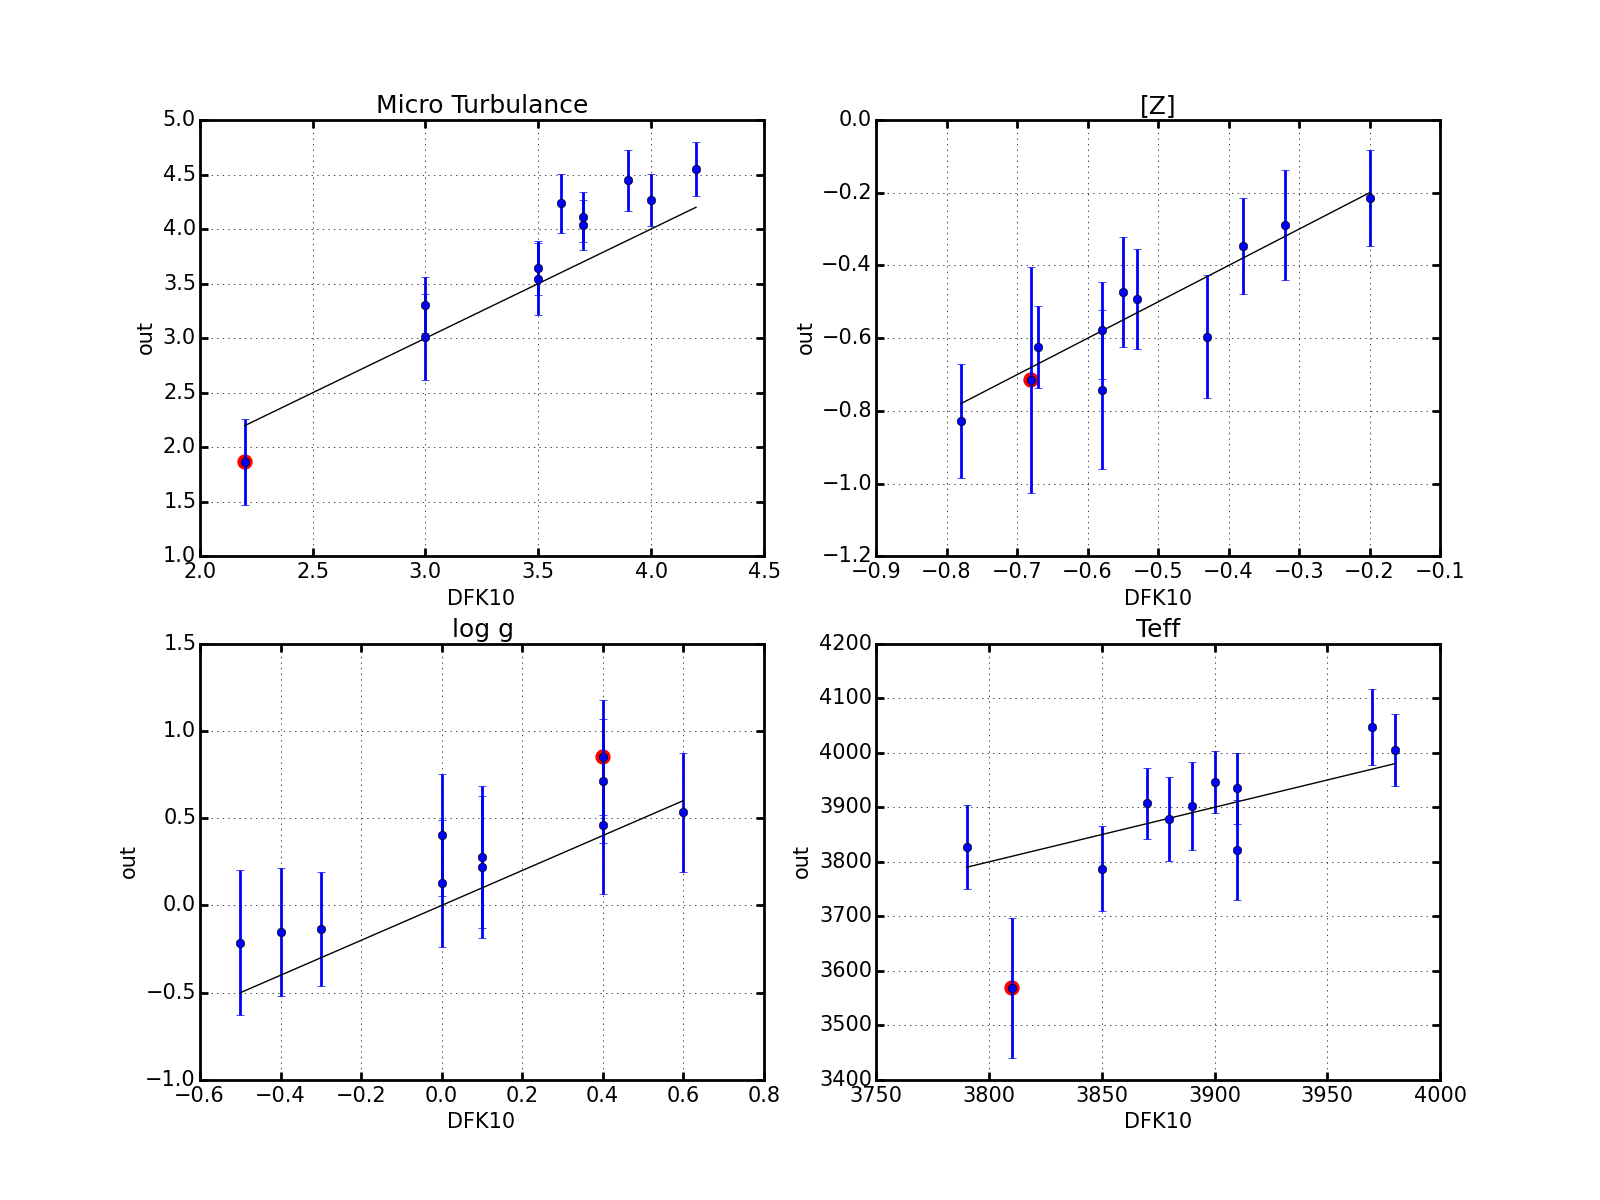
\includegraphics[width=0.65\textwidth]{JAnal/compare-DFK10}
 \caption[NGC\,300 G14]{
A comparison between the parameters derived for 27 RSGs in NGC\,300.
DFK10 results are those published in~\cite{2015ApJ...805..182G}.
\textbf{Place holder!}\label{fig:n300G14}
         }
\end{figure}

\begin{table}
\caption[Parameter comparisons G14]{Average parameters for 27 RSGs in NGC\,300 using the G14 implementation and the implementation described here
\textbf{Place holder!}\label{tb:G14}}
\scriptsize
\begin{center}
\begin{tabular}{ccc}
 \hline
 \hline
Parameter & G14 Average & Patrick Average \\
 \hline
[Z]       & $-0.52~\pm~0.16$ &  \\
T$_{\rm eff}$ & $3887~\pm~55$ &  \\
$log\,g$  & $0.1~\pm~0.3$ &  \\
$\xi$     & $3.9~\pm~0.5$ &  \\
 \hline
\end{tabular}
\end{center}
\end{table}
% section g14 (end)
% section compare (end)

\section{Conclusions} % (fold)
\label{sub:conclusions}
In this chapter I present an analysis to derive stellar parameters from RSGs using medium resolution $J$-band spectroscopy.
I detail the important aspects of this analysis including a recipe for fitting the continuum of an observed spectrum.
I describe in detail the process by which the best fit parameters and their associated errors are estimated.
I then go on to compare the results of this analysis with that of all known implementations of this analysis method and (hopefully) show that results derived between the implementations are consistent.

% subsection conclusions (end)

% % \chapter{Near-IR selection of Red Supergiants}

\textbf{Completeness:} \textbf{30\%} \\
Observations complete, still currently working with the pipeline team to fix,
the data reduction pipeline for this instrument.

\textbf{Description:} \\
This chapter will discuss how to select RSGs based on their near-IR properties.
A more robust selection criteria will be establised based on a J-band colour-
magnitude diagram.
These results will be tested on a set of observations in M33 where effectiveness
of the technique will be estimated.

These results will be compared to the recently developed \textquoteleft
Q-parameter\textquoteright.

% \chapter{Chemistry and Kinematics of NGC\,2100}\label{ch:ngc2100}

\section{Opening Remarks} % (fold)
\label{sec:opening_remarks}

This chapter is based on the study which is accepted for publication in~\cite{2016arXiv160202702P} and represents the first application of the analysis technique presented in Chapter~\ref{ch:janal}.
Although this study was conducted after that of Chapter~\ref{ch:ngc6822}, Chapters 4, 5 and 6 are orderd by their distance from the Milky Way, rather than when they were undertaken.

% section opening_remarks (end)

\section{Introduction} % (fold)
\label{sec:ngc2100intro}

Young massive clusters (YMCs\footnotemark) are important probes of the early evolution of star clusters and have increasingly been used as tracers of star formation in galaxies~\citep[e.g.][]{1995AJ....109..960W,1997AJ....114.2381M,1999AJ....118..752Z}.
Known to contain large populations of massive stars, YMCs are also important tracers of massive star formation, which is heavily clustered~\citep{2003ARA&A..41...57L,2005A&A...437..247D,2007MNRAS.380.1271P}.
In addition to being the birthplace of most of the massive stars in the Local Universe~\citep[$>200\,$M$_{\odot}$ stars in R136;][]{2010MNRAS.408..731C}, owing to the density of stars, YMCs are thought to be the birthplace of some of the rich stellar exotica
(e.g. blue stragglers, X-ray binaries and radio pulsars) found in the old population of globular clusters~\citep[GCs;][]{2010ARA&A..48..431P}.

\footnotetext{A YMC is defined as having an age of $<100\,$Myr and a stellar mass of $>10^{4}\,$M$_{\odot}$~\citep{2010ARA&A..48..431P}.}

Recently, the idea that GCs are simple stellar populations has been called into question based on chemical anomalies of light elements~\citep[C, N, O, Na and Al; e.g.][]{2012A&ARv..20...50G}.
These anomalies are considered by most authors to be the signature of multiple stellar populations within GCs.
Studying YMCs could therefore potentially help to constrain some of the proposed models for creating multiple stellar populations within GCs~\citep[e.g.][]{2014MNRAS.441.2754C}.

Investigating the link between YMCs and older clusters is an important, uncertain, factor in the evolution of young clusters.
As most stellar systems are thought to dissolve shortly after formation~\citep{2003ARA&A..41...57L}, determining how long bound systems can remain so is an important question to answer.
Studying the dynamical properties of YMCs is, therefore, an important tool to evaluate the likelihood that young clusters will survive.
In addition, the study of YMCs in different environments can help bridge the gap between the understanding of star formation in the Solar neighbourhood and that in the high-redshift Universe.


% Over the last few years, medium resolution ($R~\geq~3000$) near-IR spectroscopy has been shown to be a powerful tool to estimate stellar parameters for red supergiant stars~\citep[RSGs;][]{2010MNRAS.407.1203D}.
% RSGs are the final evolutionary stage of a massive star and, owing to their cool atmospheres~\citep[T$_{\rm eff}\sim$~4000\,K;][]{2013ApJ...767....3D}, are brightest at $\sim1.1\,\mu$m.
% In star-forming galaxies, RSGs are the most luminous near-IR sources, therefore, they can be observed out to large distances at these wavelengths.
% Given that dust extinction is intrinsically lower at near-IR wavelengths and that the next generation of ground-/space-based telescopes will be optimised for observations at these wavelengths, RSGs are likely to become increasingly attractive targets by which to study distant star-forming galaxies.

% The $J$-band analysis technique for estimating metallicities and stellar parameters of RSGs has been rigorously tested by~\cite{2014ApJ...788...58G} and~\cite{2015ApJ...806...21D}.
% These authors show that metallicities can be estimated in extragalactic systems to a high level of accuracy and to a precision of $<0.15$\,dex.

% The availability of the $K$-band multi-object spectrograph~\citep[KMOS;][]{2013Msngr.151...21S} at the Very Large Telescope (VLT), has presented new opportunities for efficient observations of samples of RSGs in external galaxies to study their distribution and build-up of metals.
% \cite{2015ApJ...803...14P} used KMOS observations to investigate the present-day metallicity of NGC\,6822 ($d$~=~0.5\,Mpc) and~\cite{2015ApJ...805..182G} determined the metallicity gradient of NGC\,300, a grand design spiral galaxy outside the Local Group ($d$~=~1.9\,Mpc), finding striking agreement with previous measurements from stars and H\,\2 regions.


\citet{2013MNRAS.430L..35G} demonstrated that, after the appearance of the first RSGs within a YMC, the overall near-IR flux from the cluster is dominated by the RSGs (F$_{J, RSG}/$F$_{J}>0.90$).
Using this result, these authors showed that the spectrum from an unresolved star cluster can be used to estimate the average properties of the RSG population of the cluster using exactly the same analysis method as for single stars.
\citet{2015ApJ...812..160L} demonstrated this with KMOS spectroscopy of three unresolved YMCs in NGC\,4038 in the Antennae ($d$~=~20\,Mpc), at Solar-like metallicity, finding good agreement with previous studies.
With a multi-object spectrograph operating on the European Extremely Large Telescope, this technique could be used to measure metallicities of individual RSGs at distances of $>10\,$Mpc and from YMCs out to potentially $>100\,$Mpc~\citep{2011A&A...527A..50E}.

NGC\,2100 is a YMC in the Large Magellanic Cloud (LMC), located near the large star-forming 30 Doradus region.
With an age of $\sim$\,20\,Myr~\citep{1991ApJS...76..185E,2015A&A...575A..62N}, and a photometric mass of $4.6~\times~10^4M_{\odot}$~\citep[assuming~\cite{1966AJ.....71...64K} profiles]{2005ApJS..161..304M}, NGC\,2100 falls within the mass and age range where the near-IR cluster light is dominated by RSGs~\citep{2013MNRAS.430L..35G}.
This is supported by the large number of RSGs identified within this cluster (see Figure~\ref{fig:targets}).

NGC\,2100 is not a cluster in isolation.
It is located in one of the most actively star-forming regions within the Local Group of galaxies.
At $\sim$\,20\,Myr old, the most massive members of this star cluster will have already exploded as supernovae.
This should have had a profound effect on the surrounding gas and dust, and has potentially shaped the surrounding LMC\,2 supershell~\citep[see][]{1999ApJ...518..298P}.

In this chapter I estimate stellar parameters from KMOS spectroscopy for 14 RSGs which appear to be associated with NGC\,2100.
Section~\ref{sec:ngc2100obs} describes the observations and data reduction, and I detail the results in Section~\ref{sec:ngc2100results}, focusing on radial velocities of the target stars where I derive the line-of-sight velocity dispersion,
the dynamical mass of NGC\,2100 and stellar parameters.
The results are discussed in Section~\ref{sec:ngc2100disc} and conclusions are presented in Section~\ref{sec:ngc2100conc}.

% section introduction (end)

\section{Observations and Data Reduction} % (fold)
\label{sec:ngc2100obs}
These observations were obtained as part of the KMOS Guaranteed Time Observations (PI: Evans 095.B-0022) in March 2015.
The observations consisted of $8\times10$\,s exposures (seeing conditions $\sim$1\farcs0) taken with the $YJ$ grating with sky offset exposures (S) interleaved between the object exposures (O) in an O,~S,~O observing pattern.
In addition, a standard set of KMOS calibration frames were obtained as well as observations of HD\,51506 (B5) as the telluric standard star.
Figure~\ref{fig:targets} shows the observed RSGs overlaid on a {\it J}-band VISTA image of the surrounding region~\citep{2011A&A...527A.116C}.

\begin{figure}
\centering
 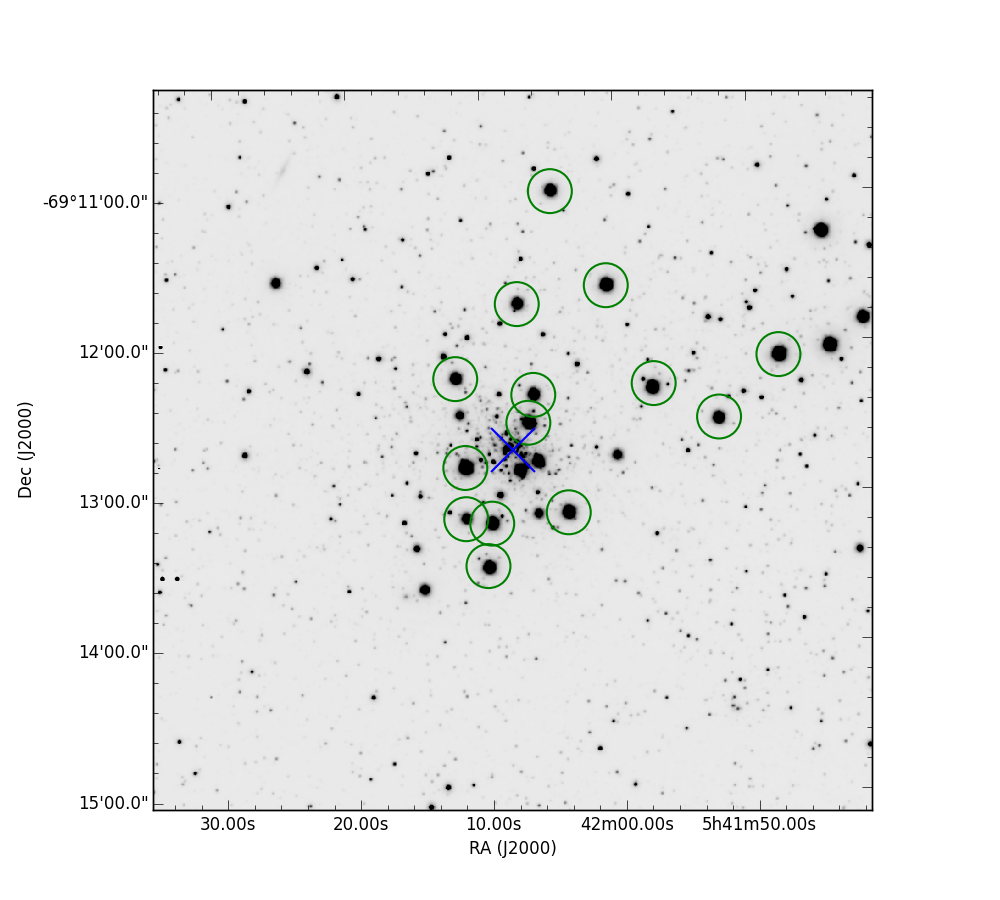
\includegraphics[width=0.65\textwidth]{ngc2100/NGC2100-targets}
 \caption[NGC\,2100 Targets]{Positions of the KMOS targets in NGC\,2100 overlaid on a VISTA $J$-band image~\citep{2011A&A...527A.116C}.
          Green circles indicate KMOS targets.
          The adopted cluster centre has been marked by a blue cross.\label{fig:targets}
          }
\end{figure}

The standard KMOS/esorex routines~\citep[SPARK;][]{2013A&A...558A..56D} were used to calibrate and reconstruct the data cubes.
Telluric correction was performed using the 24-arm telluric-correction routine using the methodology described in detail by
\citet{2015ApJ...803...14P}.
Briefly, corrections are made to the standard telluric recipe to account for slight differences in wavelength calibration between the telluric and science spectra.
This is implemented using an iterative cross-correlation approach.
Additionally, differences in the strength of the telluric features are corrected by applying a simple scaling using the equation:

\begin{equation}
  T_{2} = (T_{1} + c) / (1 + c)
\end{equation}

\noindent where $T_{2}$ is the scaled telluric-standard spectrum, $T_{1}$ is the uncorrected telluric-standard spectrum and {\it c} is the scaling parameter which is varied from {\it c}~=~$-$0.5 to {\it c}~=~0.5 in increments of 0.02.
The best value of {\it c} is chosen based on the overall standard deviation of the spectrum, i.e. the {\it c} value producing the smallest $\sigma$ is selected.
Once these corrections are accounted for, the science spectra are divided by the appropriate telluric spectrum for that particular KMOS integral field unit (IFU).


\begin{table*}
\caption{
        Observed properties of VLT-KMOS targets in NGC\,2100.\label{tb:obs-params}
        }
\scriptsize
\begin{center}
\begin{threeparttable}
\begin{tabular}{lrccccccl }
 \hline
 \hline
ID & S/N & $J$\tnote{a} & $H$\tnote{a} & $K_{\rm s}$\tnote{a} & RV (\kms) & \multicolumn{2}{c}{Probabilities\tnote{c}}& Notes\tnote{b} \\
& & & & & & P1 & P2\\
 \hline
 % Note: The table is now sorted by RA
J054147.86$-$691205.9 & 320 &\o9.525 &\o8.603 & 8.200 & 250.3\,$\pm$\,4.7 & 92 & 8\o  & D15\\
J054152.51$-$691230.8 & 200 & 10.413 &\o9.526 & 9.155 & 249.3\,$\pm$\,2.6 & 93 & 7\o  & D16\\
J054157.44$-$691218.1 & 200 &\o9.811 &\o9.036 & 8.738 & 245.6\,$\pm$\,3.5 & 90 & 10  & C2\\ % 2" off in DEC
J054200.74$-$691137.0 & 260 &\o9.900 &\o9.017 & 8.683 & 248.8\,$\pm$\,2.7 & 93 & 7\o  & C8\\
J054203.90$-$691307.4 & 250 &\o9.839 &\o8.996 & 8.740 & 251.1\,$\pm$\,2.8 & 92 & 8\o  & B4\\
J054204.78$-$691058.8 & 210 & 10.319 &\o9.427 & 9.159 & 256.1\,$\pm$\,4.0 & 74 & 26  & \ldots\\
J054206.36$-$691220.2 & 200 & 10.371 &\o9.480 & 9.159 & 255.7\,$\pm$\,4.9 & 77 & 23  & B17\\
J054206.77$-$691231.1 & 250 &\o9.977 &\o9.150 & 8.807 & 250.6\,$\pm$\,3.4 & 92 & 8\o  & A127\\
J054207.45$-$691143.8 & 200 & 10.482 &\o9.610 & 9.351 & 252.5\,$\pm$\,3.0 & 90 & 10  & C12\\
J054209.66$-$691311.2 & 240 &\o9.976 &\o9.136 & 8.841 & 254.3\,$\pm$\,4.1 & 84 & 16  & B47\\
J054209.98$-$691328.8 & 250 & 10.021 &\o9.150 & 8.823 & 250.2\,$\pm$\,3.0 & 93 & 7\o  & C32\\
J054211.56$-$691248.7 & 300 &\o9.557 &\o8.617 & 8.264 & 255.5\,$\pm$\,4.3 & 78 & 22  & B40\\
J054211.61$-$691309.2 & 150 & 10.943 & 10.090 & 9.788 & 256.6\,$\pm$\,6.1 & 72 & 28  & B46\\
J054212.20$-$691213.3 & 200 & 10.440 &\o9.622 & 9.335 & 260.0\,$\pm$\,4.8 & 34 & 66  & B22\\

% J054147.86-691205.9 0207-0134568 & 05:41:47.873 & -69:12:05.959
% J054152.51-691230.8 0207-0134683 & 05:41:52.430 & -69:12:30.410
% J054157.44-691218.1 0207-0134811 & 05:41:57.286 & -69:12:16.480 % 2" off in DEC
% J054200.74-691137.0 0208-0135292 & 05:42:00.722 & -69:11:36.925
% J054203.90-691307.4 0207-0134979 & 05:42:03.877 & -69:13:07.410
% J054204.78-691058.8 0208-0135383 & 05:42:04.762 & -69:10:58.816
% J054206.36-691220.2 0207-0135059 & 05:42:06.348 & -69:12:20.150
% J054206.77-691231.1 0207-0135069 & 05:42:06.764 & -69:12:31.245
% J054207.45-691143.8 0208-0135446 & 05:42:07.435 & -69:11:43.692
% J054209.66-691311.2 0207-0135150 & 05:42:09.647 & -69:13:11.263
% J054209.98-691328.8 0207-0135162 & 05:42:10.001 & -69:13:28.210
% J054211.56-691248.7 0207-0135205 & 05:42:11.574 & -69:12:48.770
% J054211.61-691309.2 0207-0135206 & 05:42:11.592 & -69:13:09.257
% J054212.20-691213.3 0207-0135220 & 05:42:12.182 & -69:12:13.144
\hline
\end{tabular}
\begin{tablenotes}
\item [a] Photometric data from 2MASS, with typical errors on $J$, $H$, and $K_{\rm s}$ of 0.024, 0.026 and 0.022\,mag respectively.
\item [b] Cross-identifications in final column from~\cite{1974A&AS...15..261R}.
\item [c] Probabilities $P1=P(x|\{\mu, \sigma\}_{NGC\,2100}, \{\mu, \sigma\}_{LMC-field})$,\\
                        $P2=P(x|\{\mu, \sigma\}_{LMC-field}, \{\mu, \sigma\}_{NGC\,2100})$
\end{tablenotes}
\end{threeparttable}
\end{center}
\end{table*}

% section observations (end)

\section{Results} % (fold)
\label{sec:ngc2100results}

% section results (end)

\subsection{Radial velocities and velocity dispersion} % (fold)
\label{sub:radial_velocities}
Radial velocities are estimated using an iterative cross-correlation method.
To ensure systematic shifts are removed, the observed spectra are first cross-correlated against a spectrum of the Earth's atmosphere, taken from the European Southern Observatory web pages\footnotemark, at a much higher spectral resolution than that of KMOS.
This spectrum is then degraded to the resolution of the observations using a simple Gaussian filter.
The cross-correlation is performed within the 1.140--1.155\,$\mu$m region, as a strong set of reliable telluric features dominates this region, with minimal contamination from stellar features.
The shift arising from this comparison is typically 0--10\,\kms~and is then applied to the science spectra so that they are on a consistent wavelength solution.

\footnotetext{Retrieved from http://www.eso.org/sci/facilities/paranal/\\
decommissioned/isaac/tools/spectroscopic\_standards.html}

Stellar radial velocities are estimated following a similar approach to the methods used by~\citet{2015ApJ...798...23L} and~\citet{2015ApJ...803...14P}. An initial radial-velocity estimate is found for each star from cross-correlation of the KMOS spectra with an appropriate model spectrum in the 1.16--1.22\,$\mu$m region
(selected owing to the dominance of atomic features in RSG spectra at these wavelengths).
The initial estimate is improved upon via an independent cross-correlation of the observed and model spectra for seven strong absorption lines in this region.

The quoted radial velocity for each star is the mean of these estimates, where the quoted uncertainty is the standard error of the mean
(i.e. $\sigma$/$\sqrt{n_{\rm lines}}$).
Obvious outliers (with $\delta$RVs of tens of \kms) were excluded in calculating the mean estimates; such outliers arise occasionally from spurious peaks in the cross-correlation functions from noise/systematics in the spectra.

In order to sample from the posterior probability distribution for the intrinsic velocity dispersion and mean cluster velocity (given the observed radial velocity estimates and their uncertainties), \texttt{emcee}~\citep{2013PASP..125..306F},
an implementation of the affine-invariant ensemble sampler for Markov chain Monte Carlo (MCMC) of \cite{2010CAMCS.5..65G}, is used. The likelihood function is given by

\begin{equation}
p(D|\{\sigma_{1D}, v_0\}) = \prod_i \frac{1}{\sqrt{2 \pi (\sigma_{1D}^2+ \sigma_{v, i}^2)}}  \exp{\left(\frac{-(v_i - v_0)^2}{2 (\sigma_{1D}^2+ \sigma_{v, i}^2)}\right)},
\label{eq:like}
\end{equation}

\noindent where $\sigma_{1D}$ is the intrinsic velocity dispersion of the cluster, $v_0$ is the mean cluster velocity, and the data consists of the set of radial velocity measurements $v_i$ and their uncertainties $\sigma_{v, i}$.
The intrinsic cluster dispersion is assumed to be Gaussian with no variations in the dispersion across the sample.
The systemic radial velocity ($v_0$) of the sample is estimated to be 251.6\,$\pm$\,1.1\,\kms.

Figure~\ref{fig:rvs} shows the stellar radial velocity estimates as a function of distance from the centre of the cluster, compared with the average radial velocity of $\sim$200 massive stars within the LMC from~\citet[][green dashed line]{2015A&A...584A...5E}.
To quantify the likelihood that the measured velocities are consistent with the NGC\,2100 mean cluster velocity the probability that each measured velocity is drawn from a two-component mixture of Gaussian distributions with
$P(x|\{\mu, \sigma\}_{NGC\,2100}) + P(x|\{\mu, \sigma\}_{LMC-field}) = 1$ is calculated,
where the {\it LMC-field} distribution is defined by~\cite{2015A&A...584A...5E}.
This allows calculation of the ratio of the probabilities using the equation,

\begin{equation}
    P(x|\{\mu, \sigma\}_X,\{\mu, \sigma\}_Y) = \frac{P(x|\{\mu, \sigma\}_X)}{P(x|\{\mu, \sigma\}_X) + P(x|\{\mu, \sigma\}_Y)},
\end{equation}

where $P(x|\{\mu, \sigma\}_X)$ and $P(x|\{\mu, \sigma\}_Y)$ are the Gaussian distributions centred on the NGC\,2100 systemic velocity or the LMC-field population as defined by~\cite{2015A&A...584A...5E}.

From this analysis one target (J054212.20$-$691213.3) has a measured velocity with greater probability of being drawn from the underlying distribution of massive stars rather than the distribution centred on the NGC\,2100 systemic velocity.
Excluding this target from the sample does not alter the estimation of $v_0$ or $\sigma_{1D}$ significantly, therefore this target is included for further analysis.

I conclude that all targets have a velocity consistent with membership to the LMC (as opposed to Galactic objects) and that none display compelling evidence for being excluded from membership of NGC\,2100.

The estimated $v_0$ is in reasonable agreement with previous measurements for two OB-type stars in the cluster
\citep{2015A&A...584A...5E} as well as the results from four RSGs in NGC\,2100
\citep[henceforth JT94; three of which were observed in the current study]{1994A&A...282..717J}.
Table~\ref{tb:rvs} contains the details of previous radial velocity measurements within NGC\,2100.
I conclude that there exists no significant difference between the measurements and previous estimates within NGC\,2100.
This is an additional confirmation that absolute radial velocities can be precisely measured with KMOS spectra.

\begin{figure}
 \centering
 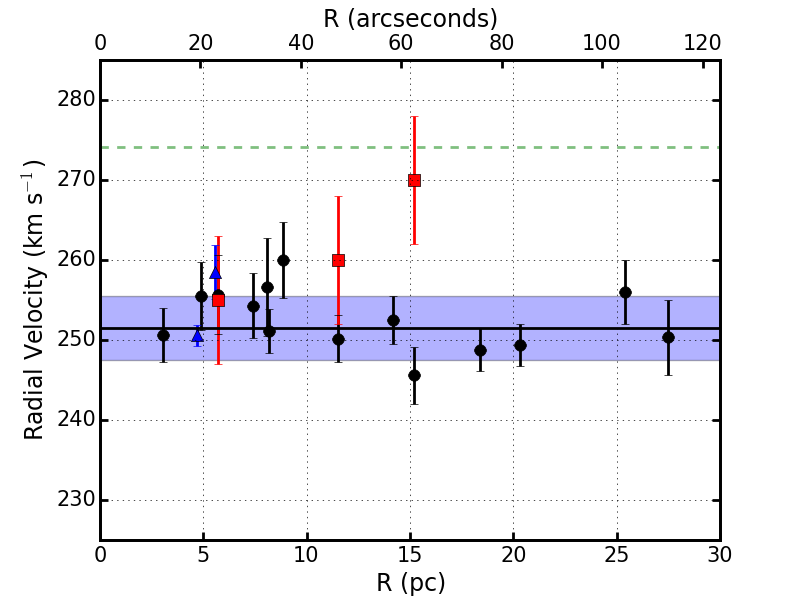
\includegraphics[width=9.0cm]{ngc2100/NGC2100-rv-v10}
 \caption[KMOS radial velocites in NGC\,2100]{Radial velocities of KMOS targets (black points) shown as a function of distance from the cluster centre.
The green dashed line shows the LMC systemic velocity of $\sim$200 massive stars from
 {\protect\citep[274.1\,$\pm$\,16.4\,\kms;][]{2015A&A...584A...5E}}.
 The solid black line shows the mean cluster velocity ($v_0$~=~251.6\,$\pm$\,1.1\,\kms) and the shaded blue region shows $v_0\,\pm\sigma_{1D}$.
 The blue triangles show estimates for two OB-type stars in NGC\,2100~\protect\citep{2015A&A...584A...5E} and the red squares show previous estimates for three targets
 {\citep{1994A&A...282..717J}}.
 The distance modulus used to produce this figure is 18.5~\citep{2013Natur.495...76P,2014AJ....147..122D}.
 \label{fig:rvs}}
\end{figure}

\begin{table*}
\begin{center}
\caption{
        Literature stellar radial-velocity measurements within NGC\,2100.\label{tb:rvs}
        }
\scriptsize
\begin{threeparttable}
\begin{tabular}{lcccll}
 \hline
 \hline
\multicolumn{2}{c}{ID} & \multicolumn{2}{c}{RV (\kms)}  & Reference & Notes \\
Lit. & current study & Lit. & current study\\
 \hline
AA$\Omega$\,30\,Dor\,407 & ---         & $258.5\pm3.4$     & \ldots        & {\cite{2015A&A...584A...5E}} &  O9.5\,II  \\
AA$\Omega$\,30\,Dor\,408 & ---         & $250.6\pm1.3$     & \ldots        & {\cite{2015A&A...584A...5E}} &  B3\,Ia    \\
R74\,B17 & J054206.36-691220.2 & $255\pm8$ & $255.7\pm4.9$ & {\cite{1994A&A...282..717J}} \\
R74\,C2  & J054157.44-691218.1 & $270\pm8$ & $245.6\pm3.5$ & {\cite{1994A&A...282..717J}} \\
R74\,C32 & J054209.98-691328.8 & $260\pm8$ & $250.2\pm3.0$ & {\cite{1994A&A...282..717J}} \\
R74\,C34 & ---         & $265\pm8$         & \ldots        & {\cite{1994A&A...282..717J}} & \\
% NGC\,2100 & ---   & $280\pm10(16)$    & \ldots        & {\cite{1972MNRAS.159..445A}} & Whole cluster\\
% NGC\,2100 & --- & $282.2\pm2.5$       & \ldots        & {\cite{1971ApJ...169..271S}} & Gas\\
% NGC\,2100 & --- & $253\pm17$          & \ldots        & {\cite{1970PhD...........F}} & \\

\hline
\end{tabular}

\begin{tablenotes}
\item ID and RV columns: the first value is from the literature and the second is from the current study.
\end{tablenotes}
\end{threeparttable}
\end{center}
\end{table*}

As shown in Figure~\ref{fig:sig1d}, the line-of-sight velocity dispersion ($\sigma_{1D}$) of NGC\,2100 is unresolved given the current data.
Therefore an upper limit on $\sigma_{1D} <$~3.9\,\kms~at the 95\% confidence level is adopted.
Figure~\ref{fig:sig1dbins} demonstrates that there is no evidence for spatial variations in the measured $\sigma_{1D}$ and it is noted that in each radial bin (which contain 5, 4 and 5 stars respectively), the measured dispersion is unresolved.


\begin{figure}
\centering
 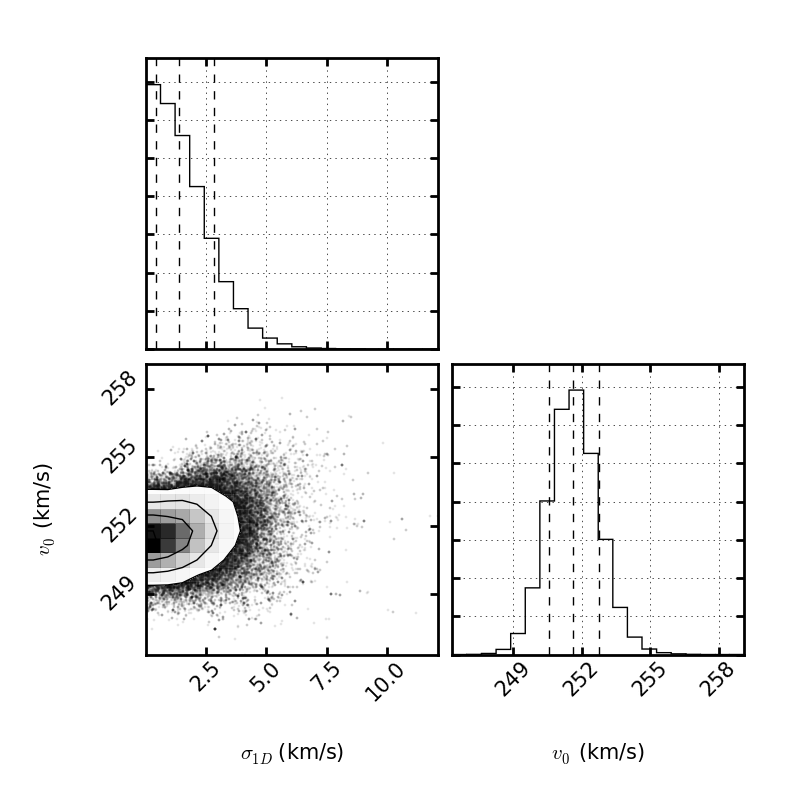
\includegraphics[width=0.65\textwidth]{ngc2100/NGC2100-sigRV-triangle}
 \caption[One- and two-dimensional projections of $\sigma_{1D}$ and $v_{0}$]{One- and two-dimensional projections of the posterior probability distributions of the line-of-sight velocity dispersion ($\sigma_{1D}$) and systemic velocity ($v_{0}$) for NGC\,2100 assuming the dispersion is Gaussian and constant over the range measured using.
 Using this method the velocity of NGC\,2100 is 251.6\,$\pm$\,1.1\,\kms.
 This figure also demonstrates that the velocity dispersion for the sample is unresolved and therefore an upper limit is placed on $\sigma_{1D} <$~3.9\,\kms~at the 95\% confidence level.
\label{fig:sig1d}
          }
\end{figure}

\begin{figure}
\centering
 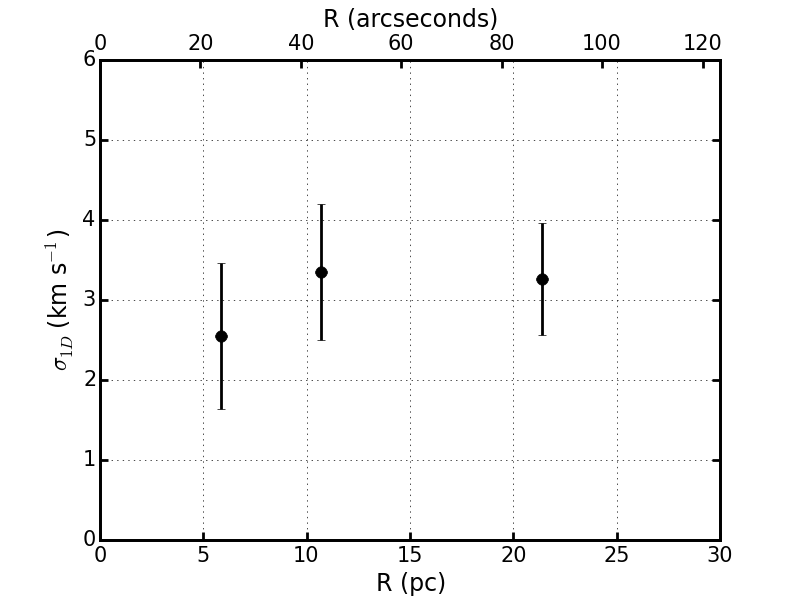
\includegraphics[width=0.65\textwidth]{ngc2100/NGC2100-sig1d-bins}
 \caption[$\sigma_{1D}$ as a function of radial distance from the cluster centre]{Upper limits to the line-of-sight velocity dispersion for the NGC\,2100 RSGs in three radial bins as a function of the distance from the centre of NGC\,2100.
 This figure demonstrates that there is no evidence for spatial variations in $\sigma_{1D}$.
 However, it is noted that in each radial bin the underlying dispersion is unresolved (see Figure~\ref{fig:sig1d}).
\label{fig:sig1dbins}
          }
\end{figure}

% section radial_velocities (end)

\subsection{Dynamical mass} % (fold)
\label{sub:dynamical_mass}
Using $\sigma_{1D}$ as an upper limit on the velocity distribution, one can calculate an upper limit on dynamical mass of the cluster using the virial equation:

\begin{equation}
  M_{dyn} = \frac{\eta\sigma_{1D}^{2}r_{\rm eff}}{G}
  \label{eq:vir}
\end{equation}

\noindent where $M_{dyn}$ is the dynamical mass and $\eta$~=~6$r_{vir}/r_{\rm eff}$~=~9.75 -- providing the density profile of the cluster is sufficiently steep~\citep{2010ARA&A..48..431P} --
where $r_{\rm eff}$~=~4.41\,pc for NGC\,2100~\citep{2005ApJS..161..304M}.
However, NGC\,2100 has a relatively shallow density profile~\citep[$\gamma$~=~$2.44\pm0.14$;][]{2003MNRAS.338...85M}
which means $\eta$~$<$~9.75.
Using $\sigma_{1D}$~=~$3.9$\,\kms~and equation~\ref{eq:vir}, an upper limit on the dynamical mass of NGC\,2100 is $M_{dyn}$~=~$15.2\times 10^{4}M_{\odot}$.
Comparing this to the photometric mass $M_{phot}$~=~$(2.3\pm1.0)\times 10^{4}M_{\odot}$~\citep{2005ApJS..161..304M},
the upper limit on the dynamical mass is larger.

As discussed by~\citet{2010MNRAS.402.1750G}, binary motions can increase the measured velocity dispersion profile~\citep[e.g. see][]{2012A&A...546A..73H}.
However, as~\citet{2010MNRAS.402.1750G} note, the mean lifetime for RSGs in binary systems is significantly decreased and, where mass transfer occurs, their number decrease dramatically~\citep{2008MNRAS.384.1109E}.
Therefore it is expected that the number of RSGs in close binaries is small~\citep{1979MNRAS.186..831F,2009ApJ...696.2014D}.
The fraction of RSGs in longer-period systems is less certain, but these would contribute substantially less to the line-of-sight velocity distribution.

These arguments suggest that the estimate for the velocity dispersion in NGC\,2100 is not significantly increased by binary motions as the target stars are expected to be (predominantly) single objects. As the true dispersion of the cluster appears to be unresolved (Figure~\ref{fig:sig1d}), it is concluded therefore that the upper limit of the dynamical mass is consistent with the published photometric mass.

Evidence in the literature suggests that J054211.61$-$691309.2 is an eclipsing binary system VV Cep~\citep{1979MNRAS.186..831F}.
However, the radial velocity of this star (256.6\,$\pm$\,6.1\,\kms) does not appear to be increased as a result of binary motions, with respect to the sample studied here.

% subsection dynamical_mass (end)

\subsection{Stellar parameters} % (fold)
\label{sub:stellar_parameters}

Stellar parameters are estimated for each target using the $J$-band analysis technique described initially by~\cite{2010MNRAS.407.1203D}
and tested rigorously by~\cite{2014ApJ...788...58G} and~\cite{2015ApJ...806...21D}.
These studies show that by using a narrow spectral window within the $J$-band one can accurately derive overall metallicities
([Z]~=~$\log$(Z/Z$_{\odot}$)) to better than
$\pm$\,0.15\,dex at the resolution of KMOS observations with S/N~$\ge~100$.
\cite{2015ApJ...803...14P} built on this by demonstrating the feasibility of this technique using KMOS spectra.

The analysis uses synthetic RSG spectra, extracted from {\sc marcs} model atmospheres~\citep{2008A&A...486..951G},
computed with corrections for non-local thermodynamic equilibrium for lines from titanium, iron, silicon and magnesium
\citep{2012ApJ...751..156B,2013ApJ...764..115B,2015ApJ...804..113B}.
The parameter ranges for the grid of synthetic RSG spectra are listed in Table~\ref{tb:mod_range}.
The synthetic spectra are compared with observations using the $\chi$-squared statistic and the synthetic spectra are degraded to the resolution and sampling of the observations.
The diagnostic spectral features used to estimate stellar parameters have equal weighting in the analysis.


Estimated stellar parameters are listed in Table~\ref{tb:stellar-params}.
Figure~\ref{fig:model_fits} shows the observed KMOS spectra (black) compared to their best-fitting models (red).
The average metallicity for the 14 RSGs is [Z]~=~$-$0.38\,$\pm$\,0.20\,dex where the large scatter is a result of the contribution from (J054211.61$-$691309.2).
Excluding this apparent outlier yields an average metallicity of [Z]~=~$-$0.43\,$\pm$\,0.10\,dex, which reduces the scatter and does not alter the result significantly.
The model fit parameters of J054211.61$-$691309.2 suggest a considerably ($\times$1.7) super-solar
metallicity.
This appears unlikely given its apparent membership of the LMC, and it is notable that the estimates for the surface gravity and microturbulence parameters are also outliers compared to the rest of the sample.
In addition, as noted above, this star was flagged as a potential eclipsing binary by~\citep{1979MNRAS.186..831F}, therefore this target is excluded from the sample in further analysis.

The average metallicity in NGC\,2100 estimated here is in good agreement with estimates of the cluster metallicity using isochrone fitting to the optical colour-magnitude diagram~\citep[$-$0.34\,dex;][]{2015A&A...575A..62N}.
The only other estimate of stellar metallicity within this cluster is from JT94
who estimated metallicities using optical spectroscopy of four RSGs.
These authors found an average metallicity for NGC\,2100 of [Fe/H]~=~$-$0.32\,$\pm$\,0.03\,dex, which is in reasonable agreement with the estimate presented here.
There are three targets in common with the current study: B17, C2 and C32
\citep[using the][nomenclature]{1974A&AS...15..261R}.
Given the differences in the analyses (i.e. optical cf. infrared, and the different models used) the estimated parameters are in reasonable agreement for all three stars
(aside from the spectroscopic gravities quoted by JT94, but with reasonable agreement with their photometric gravity estimates).

Using the same analysis technique as in this study,
\cite{2015ApJ...806...21D} estimate metallicities for nine RSGs within the LMC,
finding an average value of [Z]~=~$-$0.37\,$\pm$\,0.14\,dex, which agrees well with the estimated presented in this chapter.
In Figure~\ref{fig:TeffvsZ}, the effective temperatures and metallicities from NGC\,2100 are compared with those estimated for RSGs elsewhere in the LMC.
Good agreement is found in the distribution of temperatures from the two studies, with the average agreeing well.
The range in [Z] from the LMC population is slightly larger than that of the NGC\,2100 RSGs, which is expected when comparing a star cluster with an entire galaxy; however, the averages for the two studies agree very well.

\begin{figure*}
 %\vspace{302pt}
 \begin{center}
 \centering
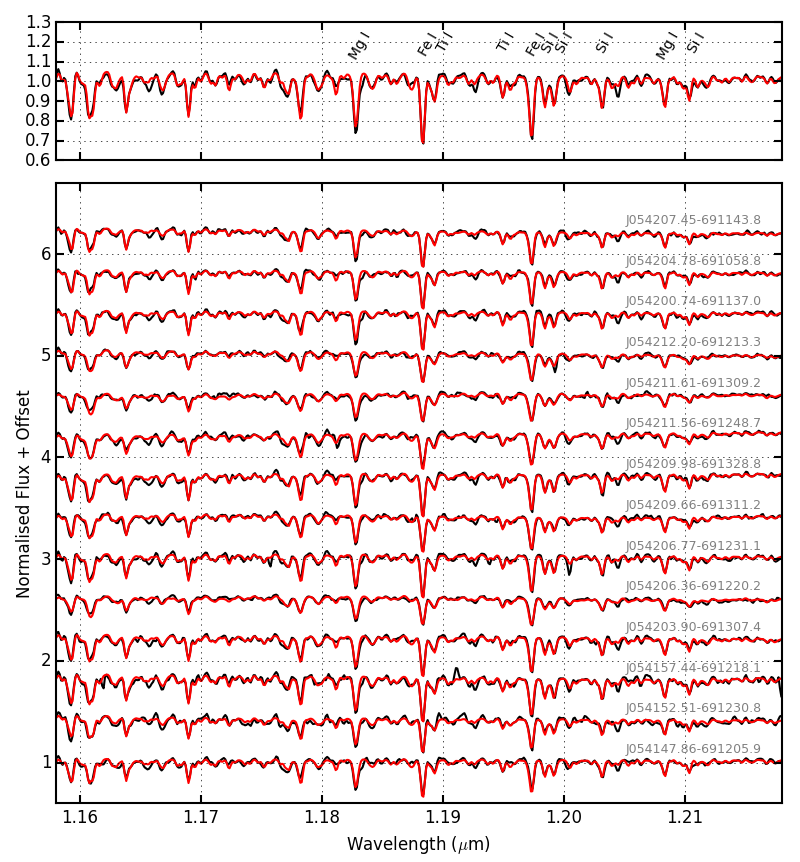
\includegraphics[width=0.75\textwidth]{ngc2100/NGC2100-model-fits}
\caption[KMOS spectra and best-fit model spectra in NGC\,2100]{KMOS spectra of RSGs in NGC\,2100 and their associated best-fit models
(black and red lines, respectively).
The upper panel shows the simulated integrated-light cluster spectrum;
the lower panel shows spectra for the individual RSGs.
The lines used for the analysis, from left-to-right by species, are
Fe\,{\scriptsize I}$\,\lambda\lambda$1.188285,
1.197305;
Mg\,{\scriptsize I}$\,\lambda\lambda$1.182819,
1.208335;
Si\,{\scriptsize I}$\,\lambda\lambda$1.198419,
1.199157,
1.203151,
1.210353;
Ti\,{\scriptsize I}$\,\lambda\lambda$1.189289,
1.194954.\label{fig:model_fits}}
\end{center}
\end{figure*}

\begin{figure}
\centering
 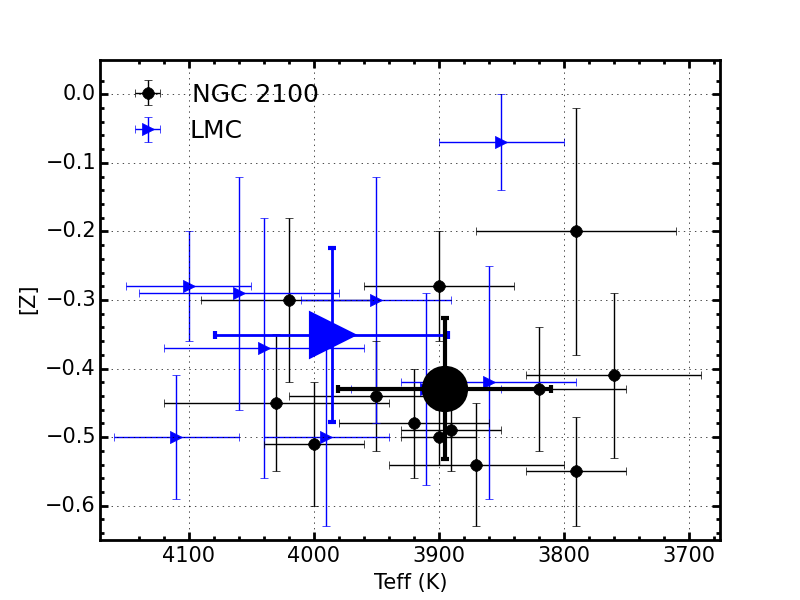
\includegraphics[width=0.65\textwidth]{ngc2100/NGC2100-TeffvsZ-2100-LMC}
 \caption[Effective temperature as a function of metallicity for NGC\,2100]{Estimated metallicities for NGC\,2100 RSGs in this study shown against effective temperature (black points).
        For comparison the distribution of LMC RSGs from~\citet[][blue triangles]{2015ApJ...806...21D} is shown with good agreement between the means of the two samples.
\label{fig:TeffvsZ}
          }
\end{figure}

\begin{table}
\caption{
Model grid used for the spectroscopic analysis.\label{tb:mod_range}
         }
\scriptsize
\begin{center}
\begin{tabular}{lccc}
 \hline
 \hline
  Model Parameter & Min. & Max. & Step size \\
 \hline
T$_{\rm eff}$ (K)       & 3400 & 4400 & 100 \\
$[$Z$]$ (dex)   & $-$1.0\o & 1.0\o  & 0.1\o\\
log\,$g$ (cgs)  & $-$1.00 & 1.00 & 0.25\\
 $\xi$ (\kms)  & \pp1.0\o & 5.0\o & 0.2\o\\
 \hline
\end{tabular}
\end{center}
\end{table}

\begin{table*}
\begin{center}
\caption{
Physical parameters determined for the KMOS targets in NGC\,2100.
\label{tb:stellar-params}
         }
\scriptsize
\begin{threeparttable}
\begin{tabular}{lc ccccl}
 \hline
 \hline
  Target  & IFU & $\xi$ (\kms) & [Z] & log\,$g$ & T$_{\rm eff}$ (K) & Notes\tnote{a}\\
  \hline
J054147.86$-$691205.9 & 7  & 3.6\,$\pm$\,0.2 & $-$0.45\,$\pm$\,0.10 & 0.10\,$\pm$\,0.16 & 4030\,$\pm$\, 90 & D15\\
J054152.51$-$691230.8 & 9  & 3.6\,$\pm$\,0.2 & $-$0.51\,$\pm$\,0.09 & 0.43\,$\pm$\,0.18 & 4000\,$\pm$\, 40 & D16\\
J054157.44$-$691218.1 & 6  & 4.9\,$\pm$\,0.1 & $-$0.44\,$\pm$\,0.08 & 0.15\,$\pm$\,0.20 & 3950\,$\pm$\, 70 & C2\\ % 2" off in DEC
J054200.74$-$691137.0 & 4  & 4.2\,$\pm$\,0.2 & $-$0.55\,$\pm$\,0.08 & 0.23\,$\pm$\,0.10 & 3790\,$\pm$\, 40 & C8\\
J054203.90$-$691307.4 & 12 & 4.5\,$\pm$\,0.2 & $-$0.49\,$\pm$\,0.06 & 0.23\,$\pm$\,0.09 & 3890\,$\pm$\, 40 & B4\\
J054204.78$-$691058.8 & 3  & 4.2\,$\pm$\,0.2 & $-$0.54\,$\pm$\,0.09 & 0.46\,$\pm$\,0.15 & 3870\,$\pm$\, 70 & \ldots\\
J054206.36$-$691220.2 & 24 & 2.8\,$\pm$\,0.4 & $-$0.20\,$\pm$\,0.18 & 0.42\,$\pm$\,0.18 & 3790\,$\pm$\, 80 & B17\\
J054206.77$-$691231.1 & 10 & 4.9\,$\pm$\,0.2 & $-$0.50\,$\pm$\,0.04 & 0.25\,$\pm$\,0.09 & 3900\,$\pm$\, 30 & A127\\
J054207.45$-$691143.8 & 2  & 4.0\,$\pm$\,0.2 & $-$0.43\,$\pm$\,0.09 & 0.45\,$\pm$\,0.17 & 3820\,$\pm$\, 70 & C12\\
J054209.66$-$691311.2 & 14 & 3.8\,$\pm$\,0.2 & $-$0.41\,$\pm$\,0.12 & 0.06\,$\pm$\,0.20 & 3760\,$\pm$\, 70 & B47\\
J054209.98$-$691328.8 & 11 & 4.8\,$\pm$\,0.1 & $-$0.48\,$\pm$\,0.08 & 0.17\,$\pm$\,0.22 & 3920\,$\pm$\, 60 & C32\\
J054211.56$-$691248.7 & 20 & 3.8\,$\pm$\,0.2 & $-$0.28\,$\pm$\,0.08 & 0.01\,$\pm$\,0.16 & 3900\,$\pm$\, 60 & B40\\
J054211.61$-$691309.2 & 18 & 2.2\,$\pm$\,0.4 & \pp0.23\,$\pm$\,0.23 & 0.65\,$\pm$\,0.19 & 3800\,$\pm$\,100 & B46\\
J054212.20$-$691213.3 & 22 & 3.3\,$\pm$\,0.2 & $-$0.30\,$\pm$\,0.12 & 0.33\,$\pm$\,0.31 & 4020\,$\pm$\, 70 & B22\\
\\
NGC\,2100 average\tnote{b} & & 4.0\,$\pm$\,0.6 & $-$0.43\,$\pm$\,0.10 & 0.25\,$\pm$\,0.15 & 3900\,$\pm$\,85\o\\
\\
Integrated-light spectrum\tnote{c}             & & 4.6\,$\pm$\,0.3 & $-$0.42\,$\pm$\,0.14 & 0.37\,$\pm$\,0.22 & 3860\,$\pm$\,85\o\\
  \hline
  \end{tabular}
\begin{tablenotes}
    \item [a] ID in final column from{~\cite{1974A&AS...15..261R}}.
    \item [b] Averages computed excluding J054211.61$-$691309.2. See text for details.
    \item [c] Simulated integrated light cluster spectrum parameters estimated excluding J054211.61$-$691309.2.
\end{tablenotes}
  \end{threeparttable}
  \end{center}
\end{table*}

% section stellar_parameters (end)

\section{Discussion} % (fold)
\label{sec:ngc2100disc}

\subsection{Stellar parameters} % (fold)
\label{sub:stellar_parameters_disc}

Luminosities have been estimated for the target stars from {\it K}-band photometry (see Table~\ref{tb:obs-params}) using the bolometric correction from~\cite{2013ApJ...767....3D} with a small contribution from interstellar extinction using E(B$-$V)~=~0.17~\citep{2015A&A...575A..62N} assuming $R_V$~=~3.5~\citep{2013A&A...558A.134D} and $A_K/A_V$~=~0.112~\citep{1985ApJ...288..618R}.
The H--R diagram for the cluster is presented in Figure~\ref{fig:HRD}.
Overlaid on this H--R diagram are {\sc syclist} stellar isochrones for SMC-like~\citep[solid lines;][]{2013A&A...558A.103G} and Solar-like~\citep[dashed lines;][]{2012A&A...537A.146E} models, where stellar rotation is 40\% of break-up velocity.
Even though the temperatures covered by the SMC-like models do not represent the distribution of temperatures observed in this study, they remain useful to constrain the age of NGC\,2100.
The Solar-like models (dashed) demonstrate that, when compared with the SMC-like models, increasing the metallicity of the sample
\begin{enumerate}
\item decreases the average temperature of the RSGs~\citep[something which is not observed by][see Chapter~\ref{ch:ngc6822}]{2015ApJ...803...14P},
\item induces so called `blue loop' behaviour for the youngest models and
\item decreases the luminosity for the youngest models.
\end{enumerate}

\begin{figure}
\centering
 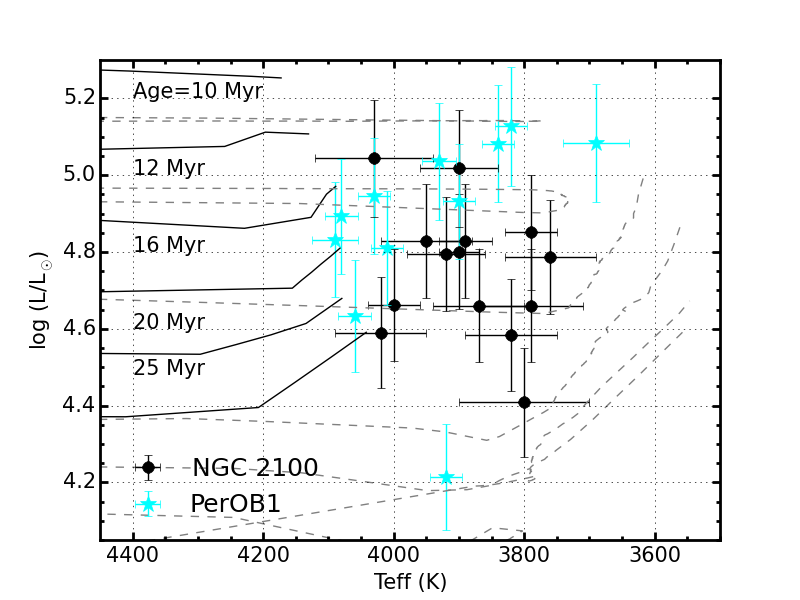
\includegraphics[width=0.65\textwidth]{ngc2100/NGC2100-HRD-perOB1}
 \caption[NGC\,2100 Hertzsprung--Russell diagram for RSGs]{Hertzsprung--Russell diagram for 14 RSGs in NGC\,2100 (black points).
  % Bolometric corrections computed using~\citet{2013ApJ...767....3D}.
  Isochrones for solar~\citep[dashed grey lines;][]{2012A&A...537A.146E} and SMC-like~\citep[solid black lines;][]{2013A&A...558A.103G} metal abundances,
  in which stellar rotation is 40\% of the break-up velocity, are shown for ages of 10-32\,Myr. For comparison, 11 RSGs from the Galactic YMC Perseus OB-1 are overlaid with cyan stars~\citep{2014ApJ...788...58G}.
  The best-fit isochrone to the observed data has an age of 20\,$\pm$\,5\,Myr for both SMC- and solar-like metallicities.
  \label{fig:HRD}
          }
\end{figure}

In addition, results for 11 RSGs from the Galactic star cluster Perseus OB-1~\citep[PerOB1;][]{2014ApJ...787..142G} are overlaid in Figure~\ref{fig:HRD} (blue stars) for which stellar parameters were estimated using the same analysis technique as in this study.
PerOB1 is a cluster with a similar mass and age~\citep[$2\times10^{4}\,$M$_{\odot}$ and 14\,Myr respectively;][]{2010ApJS..186..191C}
as NGC\,2100, and a comparison between the stellar components of these two clusters using a consistent analysis technique is useful to highlight differences in stellar evolution within clusters at this range of metallicities.

From Figure~\ref{fig:HRD}, generally, the estimated temperatures are in good agreement between the two clusters.
The median luminosity for the PerOB1 targets ($10^{4.93\pm0.15}\,$L$_{\odot}$) is slightly above that of NGC\,2100 ($10^{4.77\pm0.15}\,$L$_{\odot}$) which could represent the slight difference in the ages of the two clusters.
As PerOB1 is younger, the average mass for a RSG in the cluster will be larger than the average in NGC\,2100.
Therefore, I would expect to see higher luminosity RSGs in PerOB1.
However, the difference between the two samples is barely significant and is consistent with a constant luminosity.
The average effective temperatures for the two data sets (NGC\,2100: 3910\,$\pm$\,15\,K, PerOB1: 3940\,$\pm$\,10\,K) are in reasonable agreement, where the spread in temperatures is slightly larger for PerOB1
($\sigma_{\rm PerOB1}$~=~120\,K, $\sigma_{\rm NGC\,2100}$~=~90),
particularly so for the highest luminosity targets within the PerOB1 sample.
Overall, by comparing these two star clusters with a similar mass, age and stellar population, I conclude that there exists no significant difference in appearance on the H--R diagram of RSGs within star clusters of different metallicities.

% subsection stellar_parameters (end)

\subsection{Simulated cluster spectrum analysis} % (fold)
\label{sub:integrated_light_cluster_analysis}

The individual stars in NGC\,2100 can be used to simulate the analysis of a YMC in the more distant Universe, assuming that RSGs dominate the near-IR flux from such a cluster~\citep{2013MNRAS.430L..35G}.
\cite{2014ApJ...788...58G} use this assumption to create a simulated integrated-light cluster spectrum for PerOB1 and show that, by analysing the combined spectrum from their 11 RSGs, the resulting parameters are consistent with the average parameters estimated using the individual stars.
NGC\,2100 has a similar mass and age to PerOB1 and~\cite{2014ApJ...788...58G} analysed a similar number of RSGs to this study,
therefore, a direct comparison between the two clusters is useful to investigate potential metallicity dependencies.

To create a simulated integrated-light cluster spectrum the individual RSG spectra are summed and weighted by their $J$-band luminosities.
The resulting spectrum is then degraded to the lowest resolution spectrum of the sample using a simple Gaussian filter.
The top panel of Figure~\ref{fig:model_fits} shows the resulting integrated-light cluster spectrum.
This spectrum is then analysed in the same way described in Section~\ref{sub:stellar_parameters} for a single RSG.
The results of this analysis are what one would expect from KMOS observations of more distant YMCs where individual stars cannot be resolved.
The estimated parameters for this spectrum are, a metallicity of $-$0.35\,$\pm$\,0.07\,dex, an effective temperature of $3960\pm70\,$K,
a surface gravity of 0.64\,$\pm$\,0.19\,dex and a microturbulent velocity of $4.6\pm0.2\,$\kms~which agree well with the averages of the individual RSG parameters.

% subsection integrated_light_cluster_analysis (end)

\subsection{Velocity dispersion and dynamical mass} % (fold)
\label{sub:velocity_dispersion_Mdyn}

This study represents the first estimate of an upper limit to the line-of-sight velocity dispersion profile for NGC\,2100.
Comparing this estimate with that of other YMCs in the Local Universe is useful to ascertain if this cluster shares similar properties with other YMCs.
The properties NGC\,2100 are well matched by other clusters with similar masses and ages, particularly so with RSGC01, a Galactic YMC~\citep{2007ApJ...671..781D}.

Owing to the non-negligible contribution from measurement errors, the $\sigma_{1D}$ adopted here is an upper limit to the true dispersion within the cluster which is likely to be significantly smaller.
Using the data available, $\sigma_{1D}$~$<$~3.9\,\kms to the 95\% confidence level, however,
the true dispersion of the cluster is unresolved.

By extension, the dynamical mass estimated here is therefore also an upper limit to the true mass of the cluster.
There are several factors that could alter the value of the dynamical mass estimate.
The likely value of the $\eta$ parameter is discussed in Section~\ref{sub:dynamical_mass} and any change in this value will act to decrease the estimated dynamical mass.

% subsection velocity_dispersion (end)
% section discussion (end)

\section{Conclusions} % (fold)
\label{sec:ngc2100conc}

Using KMOS spectra of 14 RSGs in NGC\,2100 for the first time the dynamical properties of this cluster have been estimated.
Radial velocities have been estimated using KMOS, to a precision of $<~5$\,\kms, demonstrating that this instrument can be used to study the dynamical properties of star clusters in external galaxies.

An upper limit to the average line-of-sight velocity dispersion of has been estimated to be $\sigma_{1D}$~=~3.9\,\kms, at the 95\% confidence level, and no evidence is found for spatial variations.
Using the average velocity dispersion within NGC\,2100 allows an upper limit on the dynamical mass to be calculated
(assuming virial equilibrium) as $M_{dyn}$~=~$15.2\times 10^{4}M_{\odot}$.
This measurement is consistent with the literature measurement of the photometric mass~\citep{2005ApJS..161..304M} as the true dispersion is unresolved.

In addition to estimating the dynamical properties of NGC\,2100,
stellar parameters have been estimated for 14 RSGs in NGC\,2100 using the $J$-band analysis technique~\citep{2010MNRAS.407.1203D}.
The average metallicity for RSGs in NGC\,2100 is [Z]~=~$-$0.43\,$\pm$\,0.10\,dex, which agrees well with previous studies within this cluster and with studies of the young stellar population of the LMC.

The H--R diagram of NGC\,2100 is compared with that of PerOB1: a Galactic YMC with a similar age, mass and stellar population.
Using stellar parameters estimated from RSGs using the same analysis technique as in this study,
this study demonstrates that there exists no significant difference in the appearance of the H--R diagram of YMCs between these Solar- and LMC-like metallicities.

By combining the individual RSG spectra within NGC\,2100, I have simulated an integrated-light cluster spectrum and proceeded to analyse this spectrum using the same techniques for that of the individual RSGs, as RSGs dominate the cluster light in the $J$-band~\citep{2013MNRAS.430L..35G}.
The results of this technique demonstrate the potential of this analysis for integrated light spectra of more distant YMCs in low-metallicity environments.
I find good agreement using the integrated-light cluster spectrum with the average results of the individual RSGs.

% section conclusions (end)

% \chapter{KMOS Observations in NGC\,6822}
\label{ch:6822}
% \begin{figure}
%  \centering
% \centering
% \subfloat[Science One caption]{
\includegraphics[width=0.65\textwidth]{ngc6822/figure1}}
% \subfloat[Science Two caption]{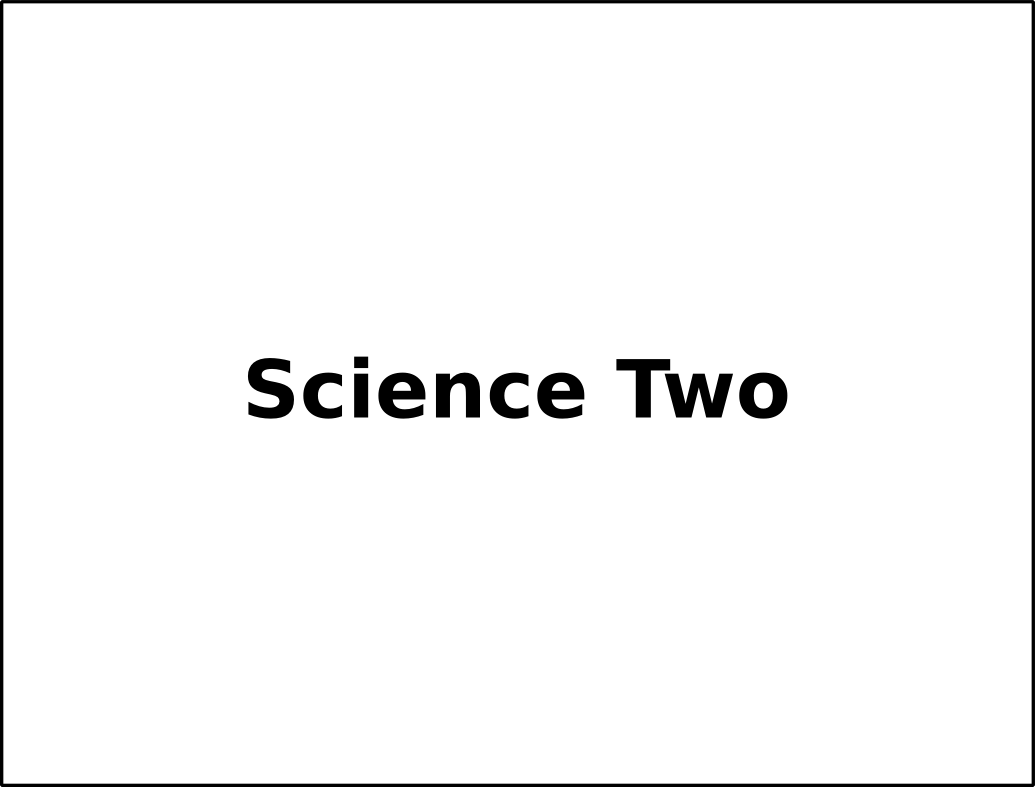
\includegraphics[width=0.65\textwidth]{ngc6822/figure2}}
% \caption[Short caption]{A long and descriptive caption about the two subfigures included above.}
% \label{fig:figures1+2}
% \end{figure}

% \section{Section One}

% \begin{table}
% \centering
% \caption{An example table, illustrating the use of the booktabs package.}
% \begin{tabular}{cccc}
% \toprule
% Here & is & a & table \\
% \midrule
% 1 & 2 & 3 & 4 \\
% 5 & 6 & 7 & 8 \\% \bottomrule
% \end{tabular}
% \label{tab:example}
% \end{table}


\section{Introduction}

\label{sec:introduction}
A promising new method to directly probe chemical abundances in external galaxies is with $J$-band spectroscopy of red supergiant (RSG) stars.
With their peak flux at
$\sim$~1\,$\mu$m and luminosities in excess of
10$^4$\,L$_\odot$, RSGs are extremely bright in the near-IR,
making them potentially useful tracers of the chemical abundances of star-forming galaxies out to large distances.
To realise this goal,
\cite{2010MNRAS.407.1203D} outlined a technique to derive metallicities of RSGs at moderate spectral resolving power
($R$~$\sim$~3000).
This technique has recently been refined using observations of RSGs in the Magellanic Clouds
\citep{2015ApJ...806...21D} and Perseus OB-1
\citep{2014ApJ...788...58G}.
Using absorption lines in the $J$-band from iron, silicon and titanium, one can estimate metallicity
([Z]~=~log\,Z/Z$_{\odot}$) as well as other stellar parameters
(effective temperature, surface gravity and microturbulence) by fitting synthetic spectra to the observations.
Owing to their intrinsic brightness,
RSGs are ideal candidates for studies of extragalactic environments in the near-IR.

To make full use of the potential of RSGs for this science, multi-object spectrographs operating in the near-IR on 8-m class telescopes are essential.
These instruments allow us to observe a large sample of RSGs in a given galaxy, at a wavelength where RSGs are brightest.
In this context, the $K$-band Multi-Object Spectrograph
\citep[KMOS;][]{2013Msngr.151...21S} at the Very Large Telescope (VLT), Chile, is a powerful facility.
KMOS will enable determination of stellar abundances for RSGs out to distances of $\sim$~10\,Mpc.
Further ahead, a near-IR multi-object spectrograph on a 40-m class telescope, combined with the excellent image quality from adaptive optics,
will enable abundance estimates for individual stars in galaxies out to tens of Mpc,
a significant volume of the local universe containing entire galaxy clusters
\citep{2011A&A...527A..50E}.

Here we present KMOS observations of RSGs in the dwarf irregular galaxy NGC\,6822,
at a distance of $\sim$~0.46\,Mpc
\citep[][and references therein]{2012AJ....144....4M}.
Chemical abundances have been determined for its old stellar population
\citep[e.g.][]{2001MNRAS.327..918T,2013ApJ...779..102K},
but knowledge of its recent chemical evolution and present-day abundances is
somewhat limited.
Observations of two A-type supergiants by
\cite{2001ApJ...547..765V} provided a first estimate of stellar abundances, finding
log\,(Fe/H)~+~12~=~7.01$\pm$0.22 and
log\,(O/H)~+~12~=~8.36$\pm$0.19, based on line-formation calculations for these elements
assuming local thermodynamic equilibrium (LTE).
A detailed non-LTE study for one of these objects confirmed the results finding
$6.96\pm 0.09$ for iron and $8.30\pm0.02$ for oxygen
\citep{2002PhDT.........3P}.
Compared to solar values of 7.50 and 8.69, respectively
\citep{2009ARA&A..47..481A},
this indicates abundances that are approximately one third solar in NGC\,6822.
A study of oxygen abundances in H\,\2 regions
\citep{2006ApJ...642..813L} found a value of $8.11\pm0.1$, confirming the low metallicity.

NGC\, 6822 is a relatively isolated Local Group galaxy, which does not seem to be associated with either M31 or the Milky Way.
It appears to have a large extended stellar halo
\citep{2002AJ....123..832L,2014ApJ...783...49H}
as well as an extended HI disk containing tidal arms and a possible HI companion
\citep{2000ApJ...537L..95D}.
The HI disk is orientated perpendicular to the distribution of old halo stars and has an associated population of blue stars
\citep{2003MNRAS.341L..39D,2003ApJ...590L..17K}.
This led \cite{2006ApJ...636L..85D} to label the system as a ``polar ring galaxy''.
A population of remote star clusters aligned with the elongated old stellar halo have been discovered
\citep{2011ApJ...738...58H,2013MNRAS.429.1039H}.
In summary, the extended structures of NGC\,6822 suggest some form of recent interaction.

In addition, there is evidence for a relatively constant star-formation history within the central 5\,kpc
\citep{2014ApJ...789..147W}
with multiple stellar populations
\citep{2006A&A...451...99B,2012A&A...540A.135S}.
This includes evidence for recent star formation in the form of a known population of massive stars, as well as a number of H\,\2 regions
\citep{2001ApJ...547..765V,2006AJ....131..343D,2009A&A...505.1027H,2012AJ....144....2L}.

In this chapter I present near-IR KMOS spectroscopy of RSGs in NGC\,6822 to investigate their chemical abundances.
In Section~\ref{sec:observations} the details of the observations are described.
Section~\ref{sec:data_reduction} describes the data reduction and
Section~\ref{sec:results} details the derived stellar parameters and investigates the spatial distribution of the estimated metallicities in NGC\,6822.
A discussion of the key results is presented in Section~\ref{sec:discussion} and
Section~\ref{sec:conclusions} concludes the chapter.

% section introduction (end)

\section{Observations}
\label{sec:observations}

\subsection{Target Selection} % (fold)
\label{sub:target_selection}

Targets were selected from optical photometry
\citep{2007AJ....134.2474M}, combined with near-IR ($JHK{_s}$) photometry
\cite[for details see][]{2012A&A...540A.135S} from the Wide-Field Camera (WFCAM) on the United Kingdom Infra-Red Telescope (UKIRT).
The two catalogues were cross-matched and only sources classified as stellar in the photometry for all filters were considered.

Our spectroscopic targets were selected principally based on their optical colours, as defined by
\cite{1998ApJ...501..153M} and
\cite{2012AJ....144....2L}.
Figure~\ref{fig:BVR} shows cross-matched stars, with the dividing line at
$(B - V)$~=~1.25~$\times (V - R)$~+~0.45.
All stars redder than this line, above a given magnitude threshold and with
$V - R >$~0.6, are potential RSGs.

Distinguishing between RSGs and the most luminous stars on the asymptotic giant branch
(AGB) is difficult owing to their similar temperatures and overlapping luminosities.
Near-IR photometry can help to delineate these populations,
with RSGs located in a relatively well-defined region in the near-IR ($J-K$) colour-magnitude diagram (CMD), as discussed by
\cite{2000ApJ...542..804N}.
The near-IR CMD from the WFCAM data is shown in
Figure~\ref{fig:JK} and was used to further inform our target selection.
Employing the updated CMD criteria from
\cite{2014A&A...562A..32C}  -- modified for the distance and reddening to NGC\,6822 --
all of our potential targets from the combined optical and near-IR criteria are (notionally) RSGs.


The combined selection methods yielded 58 candidate RSGs, from which 18 stars were observed with KMOS, as shown in Figure
\ref{fig:N6822}.
The selection of the final targets was defined by the KMOS arm allocation software {\sc karma}
\citep{2008SPIE.7019E..0TW},
where the field centre was selected to maximise the number of allocated arms,
with priority given to the brightest targets.
Optical spectroscopy of eight of our observed stars, confirming them as RSGs, was presented by
\cite{2012AJ....144....2L}.


\begin{figure}
 \centering
 \includegraphics[width=0.65\textwidth]{ngc6822/N6822_bvr}
 \caption[$B-V$ against $V-R$ two colour diagram]{
          Two-colour diagram for stars with good detections in the optical and near-IR photometry in NGC\,6822.
          The black dashed line marks the selection criteria using optical colours, as defined by
          \protect\cite{2012AJ....144....2L}.
          Red circles mark all stars which satisfied our selection criteria.
           % and our $J$-$K$, $K$ cut.
          Large blue stars denote targets observed with KMOS.
          The solid black line marks the foreground reddening vector for $E(B-V)$~=~0.22
          \protect\citep{1998ApJ...500..525S}.
         }
 \label{fig:BVR}
\end{figure}

\begin{figure}
 \centering
 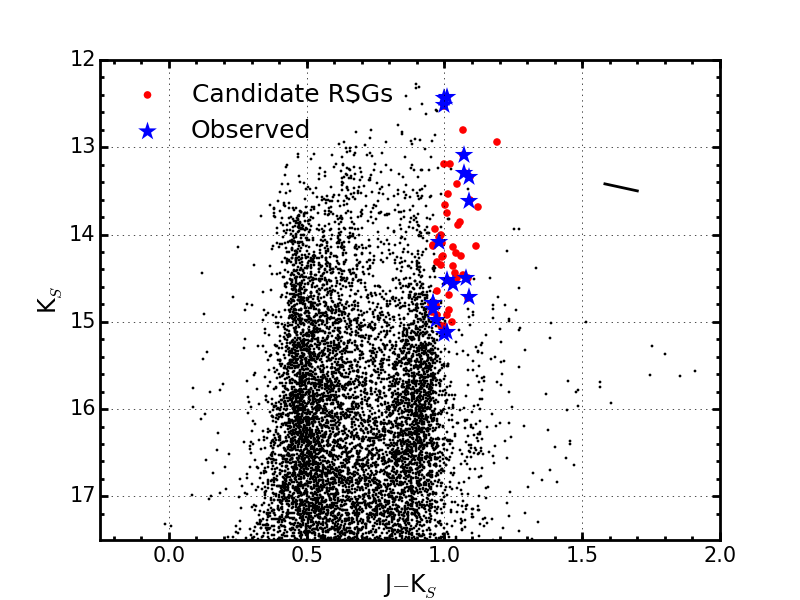
\includegraphics[width=0.65\textwidth]{ngc6822/N6822_jk}
 \caption[$J-K$ colour magnitude diagram]{
          Near-IR colour-magnitude diagram (CMD) for stars classified as stellar sources in the optical and near-IR catalogues, plotted using the same symbols as Figure~\ref{fig:BVR}.
          This CMD is used to supplement the optical selection.
          The solid black line marks the foreground reddening vector for $E(B-V)$~=~0.22
          \protect\citep{1998ApJ...500..525S}.
          % The green solid box indicates the region defined by
          % \protect\cite{2014A&A...562A..32C} as containing supergiants.
         }
 \label{fig:JK}
\end{figure}


\begin{figure}
 \centering
 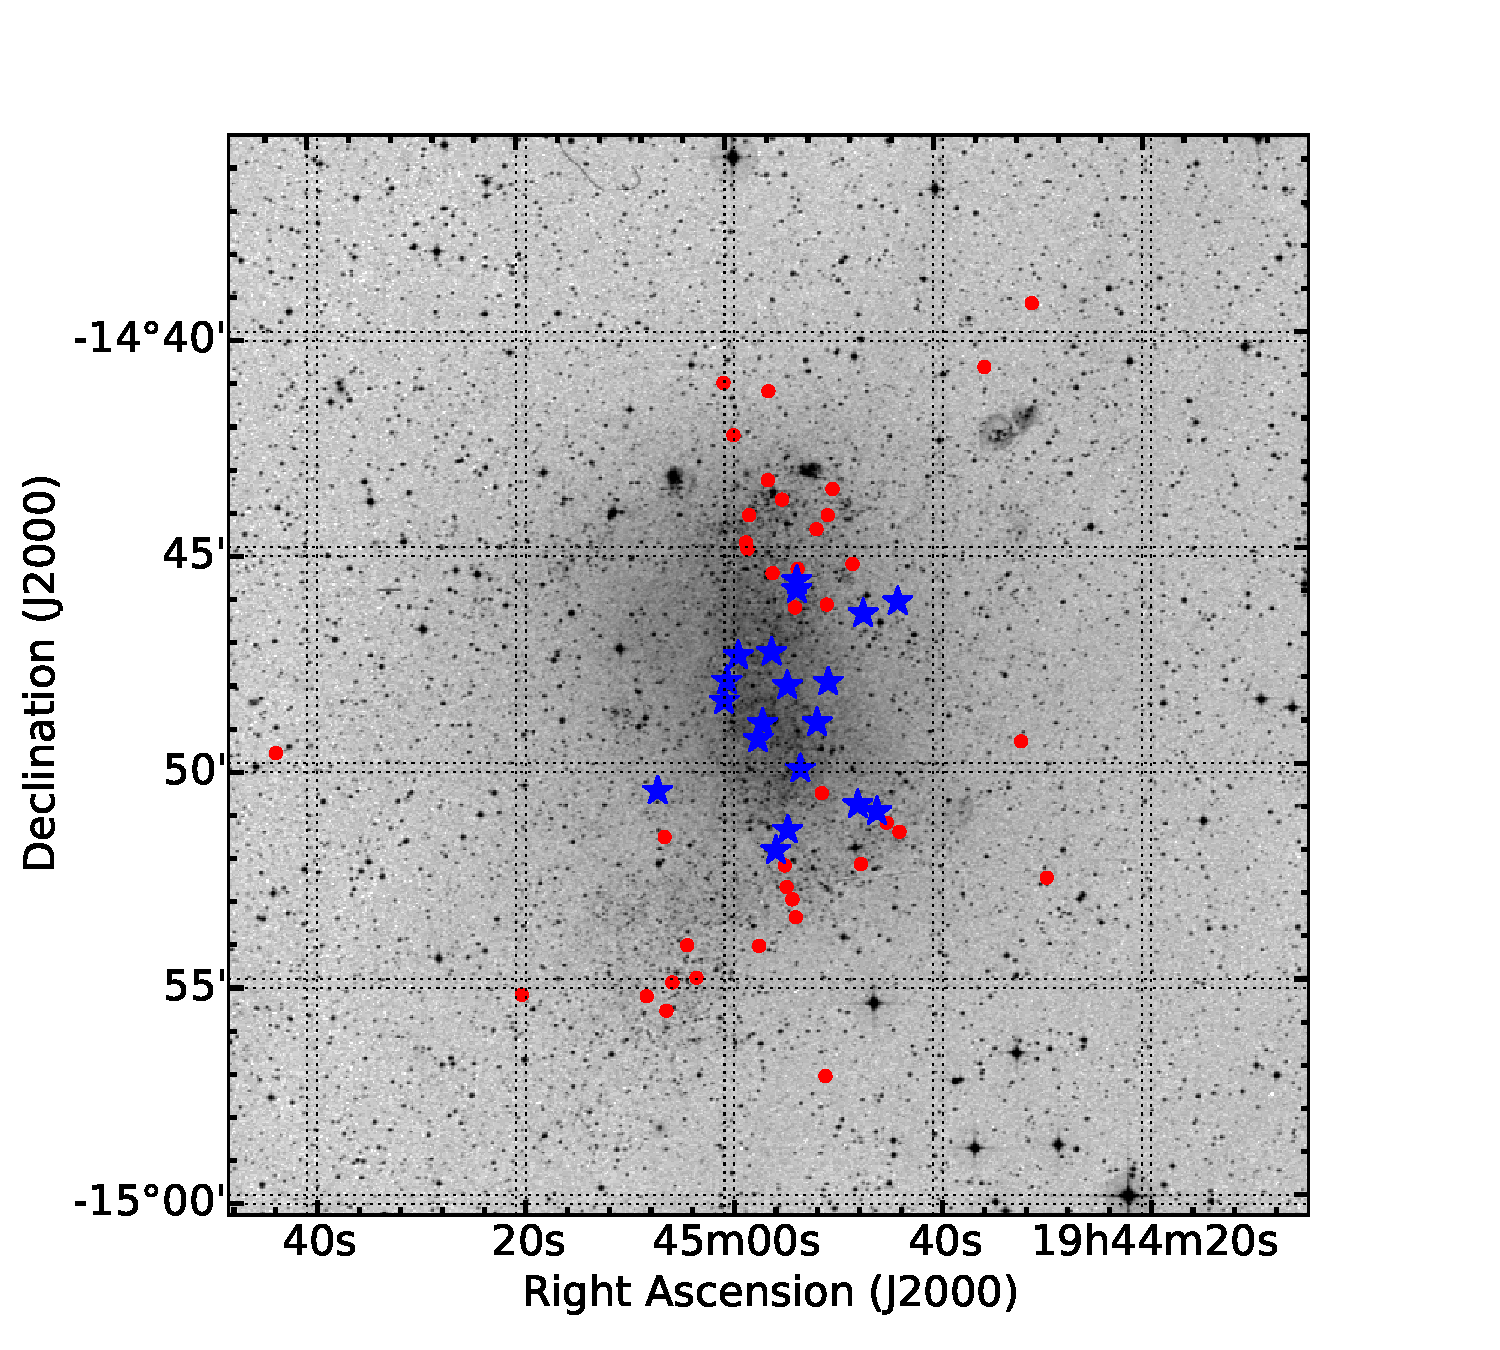
\includegraphics[width=0.65\textwidth]{ngc6822/N6822_RSGs_thesis}
 \caption[Targets identified in on-sky image]{Spatial extent of the KMOS targets over a Digital Sky Survey (DSS) image of NGC\,6822.
          Blue stars indicate the locations of the observed red supergiant stars.
          Red filled circles indicate the positions of red supergiant candidates selected using out photometric criteria (see Section~\ref{sub:target_selection}).
          }
 \label{fig:N6822}
\end{figure}

% section target_selection (end)

\subsection{KMOS Observations} % (fold)
\label{sub:observations}

The observations were obtained as part of the KMOS Science Verification program on 30 June 2013 (PI: Evans, 60.A-9452(A)),
with a total exposure time of 2400\,s
(comprising 8\,$\times$\,300\,s detector integrations).
% Observations for this study are from the new KMOS instrument on the VLT, Chile.
KMOS has 24 deployable integral-field units (IFUs) each of which covers an area of
2\farcs8 $\times$ 2\farcs8 within a 7\farcm2 field-of-view.
The 24 IFUs are split into three groups of eight, with the light from each group relayed to different spectrographs.
KMOS is described in more detail in \textbf{Chapter x.x}.

Offset sky frames
(0\farcm5 to the east) were interleaved between the science observations in an object (O), sky (S) sequence of:
O,\,S,\,O,\,O.
This observing sequence was chosen over a more standard O\,S,\,O sequence to increase time spent on science objects.
The observations were performed with the $YJ$ grating
(giving coverage from 1.02 to 1.36$\mu$m);
estimates of the mean delivered resolving power for each spectrograph (obtained from the KMOS/esorex pipeline for two arc lines) are listed in Table~\ref{tb:res}.

In addition to the science observations, a standard set of KMOS calibration frames were obtained consisting of dark, flat and arc-lamp calibrations (with flats and arcs taken at six different rotator angles).
A telluric standard star was observed with the arms configured in the science positions, i.e. using the {\em KMOS\_spec\_cal\_stdstarscipatt} template in which the standard star is observed sequentially through all IFUs.
The observed standard was HIP97618, with a spectral type of B6\,III
\citep{1988mcts.book.....H}.

A summary of the observed targets is given in
Table~\ref{tb:obs-params}.
A signal-to-noise (S/N) ratio of $>~100$ per resolution element is required for satisfactory results from this analysis method
\citep[see][]{2014ApJ...788...58G}.
We estimated the S/N ratio of the spectra by comparing the counts in the brightest spatial pixels
(within the 1.15-1.22$\mu$m region) of each source with the counts in equivalent spatial pixels in the corresponding sky exposures
(between the sky lines).
The S/N estimated is knowingly an underestimate of the true S/N achieved.

% \footnotetext{http://www.usm.uni-muenchen.de/people/wegner/kmos/en/karma.php}

\begin{table*}
\caption{Measured velocity resolution and resolving power across each detector.\label{tb:res}}
\scriptsize
\begin{center}
\begin{tabular}{crcccc}
\hline
\hline
Det. & IFUs & \multicolumn{2}{c}{Ne\,\lam1.17700\,$\mu$m}
            & \multicolumn{2}{c}{Ar\,\lam1.21430\,$\mu$m} \\
 & & FWHM [\kms] & $R$ & FWHM [\kms] & $R$ \\
  \hline
1 & 1-8 &  \a88.04\,$\pm$\,2.67 & 3\,408\,$\pm$\,103 &
           \o85.45\,$\pm$\,2.67 & 3\,511\,$\pm$\,110 \\
2 & 9-16 & \a82.83\,$\pm$\,2.48 & 3\,622\,$\pm$\,108 &
           \o80.30\,$\pm$\,3.05 & 3\,736\,$\pm$\,142 \\
3 & 17-24 & 103.23\,$\pm$\,2.73 & 2\,906\,$\pm$\,77\a &
            101.25\,$\pm$\,2.99 & 2\,963\,$\pm$\,87\a \\
\hline
\end{tabular}
\end{center}
\end{table*}

\begin{sidewaystable}
\caption[Summary of VLT-KMOS targets in NGC\,6822]{Summary of VLT-KMOS targets in NGC\,6822.\label{tb:obs-params}}
\scriptsize
\begin{threeparttable}
\centering
\begin{tabular}{lrcccccccccl}
 \hline
 \hline
ID & S/N & $\alpha$ (J2000) & $\delta$ (J2000) & $B$ & $V$ & $R$ & $J$ & $H$ & $K_{\rm s}$ & RV (\kms) & Notes \\
 \hline
NGC6822-RSG01 & 223 &   19:44:43.81  &  $-$14:46:10.7  &  20.83  &  18.59  &  17.23  &  14.16  &  13.37  &  13.09  &  $-$63.8$\pm$3.2 & Sample\\
NGC6822-RSG02 & 120 &   19:44:45.98  &  $-$14:51:02.4  &  20.91  &  18.96  &  17.89  &  15.53  &  14.72  &  14.52  &  $-$60.6$\pm$5.5 & Sample\\
NGC6822-RSG03 &  94 &   19:44:47.13  &  $-$14:46:27.1  &  21.30  &  19.41  &  18.41  &  16.13  &  15.35  &  15.12  &  $-$69.8$\pm$6.5 \\
NGC6822-RSG04 & 211 &   19:44:47.81  &  $-$14:50:52.5  &  20.74  &  18.51  &  17.22  &  14.37  &  13.58  &  13.30  &  $-$65.5$\pm$4.4 & LM12 (M1), Sample \\
NGC6822-RSG05 & 104 &   19:44:50.54  &  $-$14:48:01.6  &  20.83  &  18.95  &  17.97  &  15.75  &  14.98  &  14.79  &  $-$74.8$\pm$5.0 \\
NGC6822-RSG06 & 105 &   19:44:51.64  &  $-$14:48:58.0  &  21.33  &  19.45  &  18.32  &  15.81  &  14.95  &  14.72  &  $-$65.3$\pm$6.0 \\
NGC6822-RSG07 & 145 &   19:44:53.46  &  $-$14:45:52.6  &  20.36  &  18.43  &  17.38  &  15.06  &  14.30  &  14.08  &  $-$53.8$\pm$5.1 & LM12 (M4.5), Sample \\
NGC6822-RSG08 & 103 &   19:44:53.46  &  $-$14:45:40.1  &  20.88  &  19.14  &  18.17  &  15.95  &  15.16  &  14.98  &  $-$51.6$\pm$4.1 & LM12 (K5), Sample \\
NGC6822-RSG09 & 201 &   19:44:54.46  &  $-$14:48:06.2  &  20.56  &  18.56  &  17.35  &  14.43  &  13.67  &  13.34  &  $-$47.4$\pm$2.1 & LM12 (M1), Sample\\
NGC6822-RSG10 & 302 &   19:44:54.54  &  $-$14:51:27.1  &  19.29  &  17.05  &  15.86  &  13.43  &  12.66  &  12.42  &  $-$75.7$\pm$3.5 & LM12 (M0), Sample \\
NGC6822-RSG11 & 327 &   19:44:55.70  &  $-$14:51:55.4  &  19.11  &  16.91  &  15.74  &  13.43  &  12.70  &  12.43  &  $-$59.3$\pm$4.0 & LM12 (M0), Sample \\
NGC6822-RSG12 & 100 &   19:44:55.93  &  $-$14:47:19.6  &  21.43  &  19.56  &  18.52  &  16.14  &  15.33  &  15.14  &  $-$39.2$\pm$4.6 & LM12 (K5) \\
NGC6822-RSG13 & 106 &   19:44:56.86  &  $-$14:48:58.5  &  21.05  &  19.06  &  18.04  &  15.81  &  15.05  &  14.85  &  $-$55.7$\pm$7.4 \\
NGC6822-RSG14 & 284 &   19:44:57.31  &  $-$14:49:20.2  &  19.69  &  17.41  &  16.20  &  13.52  &  12.76  &  12.52  &  $-$84.2$\pm$1.9 & LM12 (M1), Sample \\
NGC6822-RSG15 & 124 &   19:44:59.14  &  $-$14:47:23.9  &  21.30  &  19.17  &  18.05  &  15.58  &  14.74  &  14.50  &  $-$86.9$\pm$6.6 \\
NGC6822-RSG16 & 107 &   19:45:00.24  &  $-$14:47:58.9  &  21.27  &  19.20  &  18.10  &  15.60  &  14.80  &  14.57  &  $-$67.7$\pm$3.1 \\
NGC6822-RSG17 & 167 &   19:45:00.53  &  $-$14:48:26.5  &  20.84  &  18.75  &  17.51  &  14.70  &  13.86  &  13.61  &  $-$64.8$\pm$4.2 & Sample\\
NGC6822-RSG18 & 104 &   19:45:06.98  &  $-$14:50:31.1  &  21.06  &  19.12  &  18.06  &  15.74  &  14.94  &  14.78  &\a$-$33.8$\pm$11.7& Sample\\
\hline
\end{tabular}

\begin{tablenotes}
  \item Optical data from
  \protect\cite{2007AJ....134.2474M}, with typical photometric uncertainty 0.016, 0.006, 0.010 in $B, V$ and $R$ bands respectively.
  Near-IR data from the UKIRT survey
  \protect\cite[see][for details]{2012A&A...540A.135S}, with typical errors 0.015, 0.010, 0.012, in $J, H$ and $K$ bands respectively.
  Targets observed by
  \protect\cite{2012AJ....144....2L}
  are indicated by \textquoteleft
  LM12\textquoteright~ in the final column (with their spectral classifications in parentheses).
  Targets used for abundance analysis are indicated by the comment
  \textquoteleft Sample\textquoteright
  .
\end{tablenotes}
\end{threeparttable}
\end{sidewaystable}


% subsection KMOS observations (end)
% section observations (end)

\section{Data Reduction} % (fold)
\label{sec:data_reduction}

The observations were reduced using the recipes provided by the Software Package for Astronomical Reduction with KMOS
\citep[SPARK;][]{2013A&A...558A..56D}.
The standard KMOS/esorex routines were used to calibrate and reconstruct the science and standard-star data cubes as outlined by
\cite{2013A&A...558A..56D}.
Sky subtraction was performed using the standard KMOS recipes and telluric correction was performed using two different strategies.
Throughout the following analysis all spectra have been extracted from their respective data cubes using a consistent method (i.e. the optimal extractions within the pipeline).

\subsection{KMOS/esorex pipeline} % (fold)
\label{sub:kmos_esorex_pipeline}

The KMOS/esorex pipeline performs the initial calibrations by using a set of dark, flat and arc-lamp calibrations.
These calibrations are all performed on raw KMOS images which contain 14$\times$14 spectra from each IFU from the three spectrographs.
The flat-field calibrations allow one to trace the spatial coordinates of each spectrum on the raw images.
This information is then combined with the wavelength calibration information,
obtained from the arc-lamp calibrations, to give a 14$\times$14$\times$2056 3-D spectrum for each IFU across the detector.
A snapshot of the 14$\times$14 spatial pixels is shown in Figure~\ref{fig:IFU_snapshot}.
When reducing multiple exposures of a single object, this cube is then combined to produce the final data cube.

There are many routines with which to extract spectra from this final data cube.
The simplest way to do this is to take the single brightest spectral pixel within the cube and extract a spectrum from that.
However, higher signal-to-noise can be achieved by extracting the spectrum from a circular pixel mask centred on the brightest pixel, where each pixel is weighted by the integrated flux in that pixel.
However, within each IFU, the resolution of the spectrum varies between spatial pixels.
Therefore, in order to combine the spectra more precisely, one must first standardise the resolution across the IFU before combining~\citep{2015ApJ...805..182G}.

% subsection kmos_esorex_pipeline (end)

\subsection{Sky Subtraction} % (fold)
\label{sub:sky_subtraction}

Sky subtraction is performed within the pipeline before IFU reconstruction where the science frame is matched with its nearest in time sky frame.
Initial inspection of the extracted stellar spectra revealed minor residuals from the sky subtraction process.
Reducing these cases with the \textquoteleft sky\_tweak\textquoteright
~option within the KMOS/esorex reduction pipeline was ineffective to improve the subtraction of these features.
Any residual sky features could potentially influence our results by perturbing the continuum placement within the model fits, which is an important aspect of the fitting process
\citep[see][for more discussion]{2014ApJ...788...58G,2015ApJ...806...21D}.
Thus, pending a more rigorous treatment of the data
(e.g. to take into account the changing spectral resolution across the array),
we exclude objects showing sky residuals from our analysis.
Of the 18 observed targets, 11 were used to derive stellar parameters
(as indicated in Table~\ref{tb:obs-params}).

\subsubsection{In-house Sky Subtraction} % (fold)
\label{sub:in_house_sky_subtraction}

An alternative method of sky subtraction would to to subtract the sky from spatial pixels within the object IFU.
This is possible as within each IFU the target does not extend over the entire set of spatial pixels as Figure~\ref{fig:IFU_snapshot} demonstrates.
Using a collection of these spatial pixels which contain little or no object flux can be a potential method for sky subtraction.
Clearly this method has large potential benefits with respect to observing efficiency as less sky exposures would be needed for a given observing run.
Theoretically, the sky subtraction from a region which is nearer in space to the object in question is beneficial in two different ways:
\begin{enumerate}
  \item The sky being subtracted more closely represents the sky background which the object is contaminated with.
For comparison, during the sky exposures the telescope is offset by $\sim$~10 arc-minutes, therefore, this sky exposure samples an intrinsically different atmospheric column when compared to the science exposure.
Even though the differences in the sky lines on this spatial scale is small, as the signal originating from the sky is roughly an order of magnitude larger than that of our object, a small sky residual could affect the shape and/or strength of a genuine stellar feature.
% Quantify this!
\item The region of the host galaxy which the target object occupies will often contain contaminating flux.
By sampling a region of space closer to the position of the target object, the underlying galaxy flux will be more accurately subtracted.
\end{enumerate}

However, an inherent issue with this method of sky subtraction is that one may well remove some of the object flux in this process.
Additionally, (as mentioned in~\ref{sub:kmos_esorex_pipeline}) there is know to exist a slight difference in resolution over the spatial extent of the IFU which could make comparisons between spatial pixels complicated.
By standardising the resolution across the IFU one can potentially obtain a more reliable sky subtraction at the expense of the resolution of the spectrum.


\begin{figure}
 \centering

\includegraphics[width=0.55\textwidth]{ngc6822/N6822_RSG17-snapshot}
 \caption[IFU Snapshot]{
          Snapshot of a reconstructed KMOS IFU (at $\lambda$~=~1.16\,$\mu$m) containing the science target NGC6822-RSG17.
          Darker shades indicate higher flux.
          This image serves to demonstrate that the target objects do not entirely fill the KMOS IFU.
          This therefore, presents the possibility for using several pixels which do not contain flux from the object in the sky subtraction process.
          }
 \label{fig:IFU_snapshot}
\end{figure}

  % subsection in_house_sky_subtraction (end)

% subsection sky_subtraction (end)
\subsection{Telluric Correction} % (fold)
\label{sub:telluric_correction}

One of the most important stages within the data reduction process for spectroscopic observations from ground-based observatories concerned with measuring absorption, rather than emission, features is the correction for the effects of the Earth's atmosphere.
As starlight passes through the atmosphere it is absorbed and re-emitted by various different molecules.
These strong molecular features contaminate and blend genuine stellar features.
In order to recover the stellar features a spectrum is derived which contains only the atmospheric absorption features.
This spectrum is then used to correct the science spectrum.
% To illustrate this I could show a plot of the transmission model in the near-IR

Typically, one generates a telluric spectrum by observing an additional star of known spectral type.
If the stellar features are well characterised for this spectral type, any additional features are assumed to be owing to the Earth's atmosphere.
The spectral type is usually chosen to minimize the number of stellar features present in the region of interest.
In the $J$-band an A0V star has few lines of note and is therefore a good choice of telluric standard star in this regime.
% Show a plot of an A0V star in the near-IR
This method of telluric correction is robust and well tested and is the preferred method for many different studies.
However, it does have some fairly fundamental limitations which include the fact that it is impossible to sample precisely the same atmospheric column in both the science and telluric observations, as well as the additional time it takes to observe a standard star.

Recently, a tool for telluric correction which does not require standard star observations has been developed and tested on some VLT instruments~\citep{2015A&A...576A..77S}.
This package uses atmospheric modelling techniques to derive a telluric spectrum.
The package is briefly explained in section~\ref{sub:molecfit},
however, see~\citet{2015A&A...576A..77S} for a more thorough description.


% subsection telluric_correction (end)

\subsection{Three-arm vs 24 arm Telluric Correction} % (fold)
\label{sub:three_arm_vs_24_arm_telluric_correction}

The default template for telluric observations with KMOS is to observe a standard star in one IFU in each of the three spectrographs.
However, there is an alternative template which allows users to observe a standard star in each of the 24 IFUs.
This strategy should provide an optimum telluric correction for the KMOS IFUs but reduces observing efficiency.

A comparison between the two methods in the $H$-band was given by
\cite{2013A&A...558A..56D},
who concluded that using the more efficient three-arm method was suitable for most science purposes.
However, an equivalent analysis in the $YJ$-band was not available.
To determine if the more rigorous telluric approach is required for our analysis,
we observed a telluric standard star (HIP97618) in each of the 24 IFUs.
This gave us the data to investigate both telluric correction methods and to directly compare the results.

We first compared the standard-star spectrum in each IFU with that used by the pipeline routines for the three-arm template in each of the spectrographs.
Figure~\ref{fig:IFU_compare} shows the differences between the standard-star spectra across the IFUs,
where the differences in the $YJ$-band are comparable to those in the $H$-band
\cite[cf. Fig.7 from][]{2013A&A...558A..56D}.
The qualitative agreement between the IFUs in our region of interest (1.16-1.22$\mu$m) is generally very good.


\begin{figure*}
 \centering
 \begin{center}
 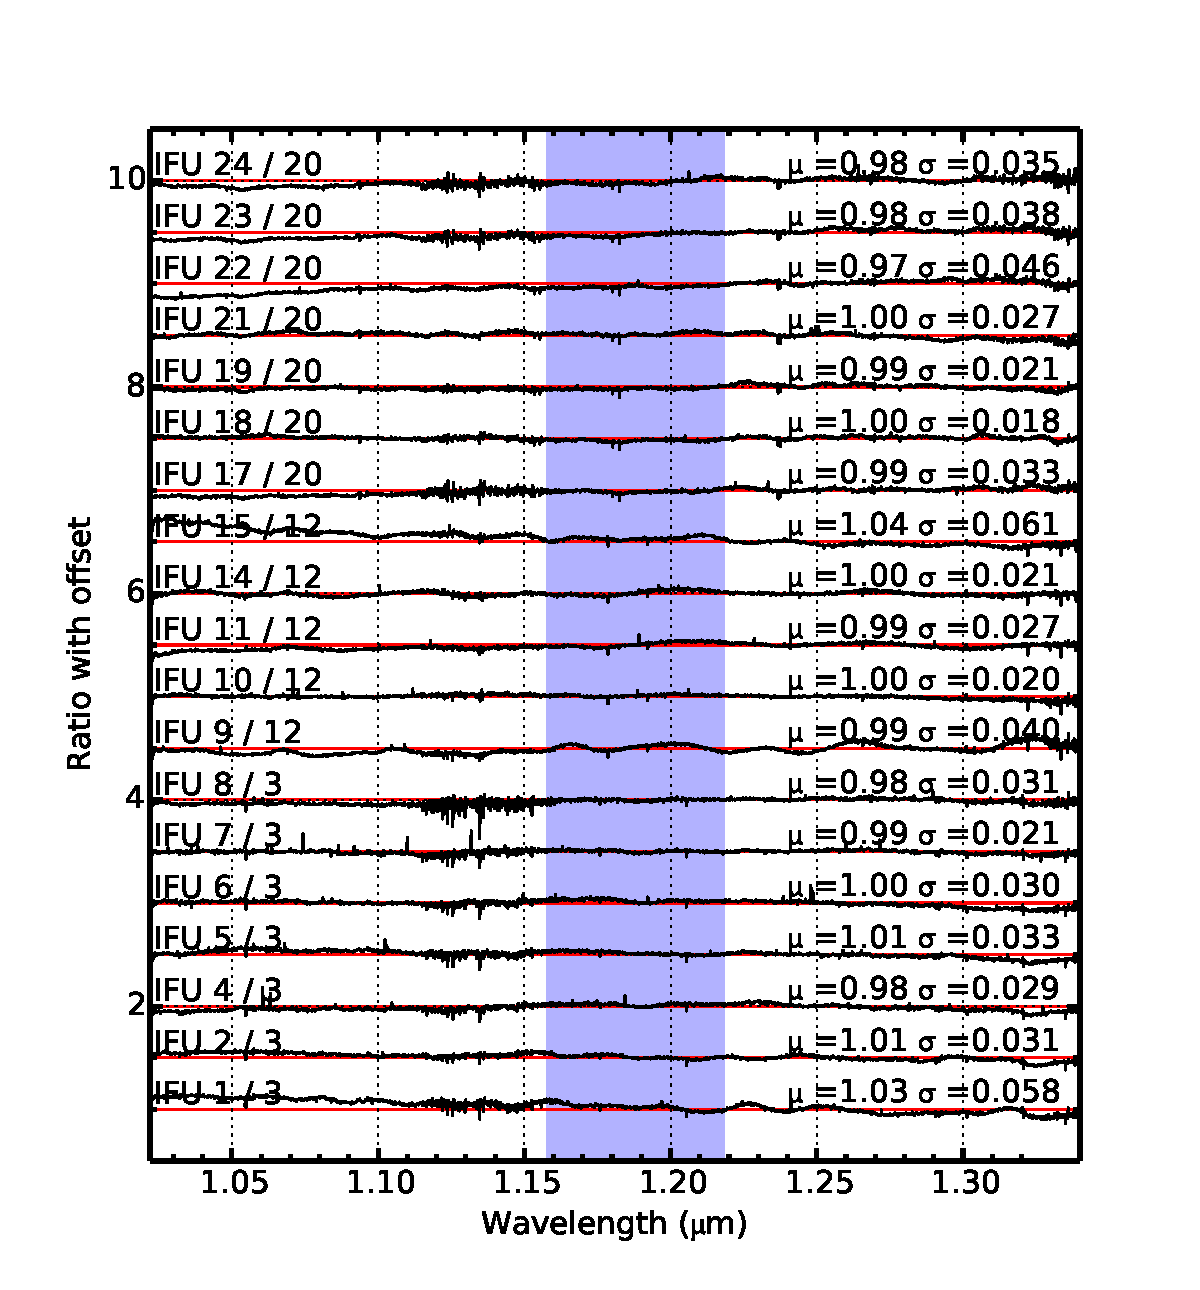
\includegraphics[width=12.0cm]{ngc6822/N6822_t_compare}
 \caption[Comparison of uniformity IFU spectra]{
    Comparison of $J$-band spectra of the same standard star in each IFU.
    The ratio of each spectrum compared to that from the IFU used in the three-arm telluric method is shown,
    with their respective mean and standard deviation ($\mu$ and $\sigma$).
    Red lines indicate $\mu$~=~1.0, $\sigma$~=~0.0 for each ratio.
    The blue shaded area signifies the region used in our analysis,
    within which, the discrepancies between the IFUs are generally small.
    This is reflected in the standard deviation values when only considering this region.
    (IFUs 13 and 16 are omitted as no data were taken with these IFUs.) \label{fig:IFU_compare}
          }
 \end{center}
\end{figure*}

To quantify the difference the two telluric methods would make to our analysis,
we performed the steps described in
Section~\ref{sub:ngc6822_telluric_correction} for both templates.
We then used the two sets of reduced science data
(reduced with both methods of the telluric correction) to compute stellar parameters for our targets.
The results of this comparison are detailed in Section
\ref{sub:telluric_comparison}.

% subsection three_arm_vs_24_arm_telluric_correction (end)

\subsection{Telluric Correction Implementation} % (fold)
\label{sub:ngc6822_telluric_correction}

To improve the accuracy of the telluric correction,
for both methods mentioned above,
we implemented additional recipes beyond those of the KMOS/esorex pipeline.
These recipes were employed to account for two effects which could potentially degrade the quality of the telluric correction.
The first corrects for any potential shift in wavelength between each science spectrum and its associated telluric standard.
The most effective way to implement this is to cross-correlate each pair of science and telluric-standard spectra.
Any shift between the two is then applied to the telluric standard using a cubic-spline interpolation routine.

The second correction applied is a simple spectral scaling algorithm.
This routine corrects for differences in line intensity of the most prominent features common to both the telluric and science spectra.
To find the optimal scaling parameter the following formula is used,

\begin{equation} \label{eq:shiftandres}
T_{2} = (T_{1} + c) / (1 + c),
\end{equation}

\noindent where $T_{2}$ is the corrected telluric-standard spectrum,
$T_{1}$ is the initial telluric standard spectrum and $c$ is the scaling parameter.

To determine the required scaling,
telluric spectra are computed for $-0.5<c<0.5$, in increments of 0.02
(where a perfect value, i.e. no difference in line strength, would be $c$~=~0).
Each telluric spectrum is used to correct the science data and the standard deviation of the counts across the spectral region is computed for each corrected spectrum.
The minimum value of the standard-deviation matrix defines the optimum scaling.
For this algorithm, only the region of interest for our analysis is considered
(i.e. 1.16-1.22\,$\mu$m).

The final set of telluric-standard spectra from the KMOS/esorex reductions were modified using these additional routines and were then used to correct the science observations for the effects of the Earth's atmosphere.



\begin{figure*}
 \centering
 %\vspace{302pt}
 \begin{center}
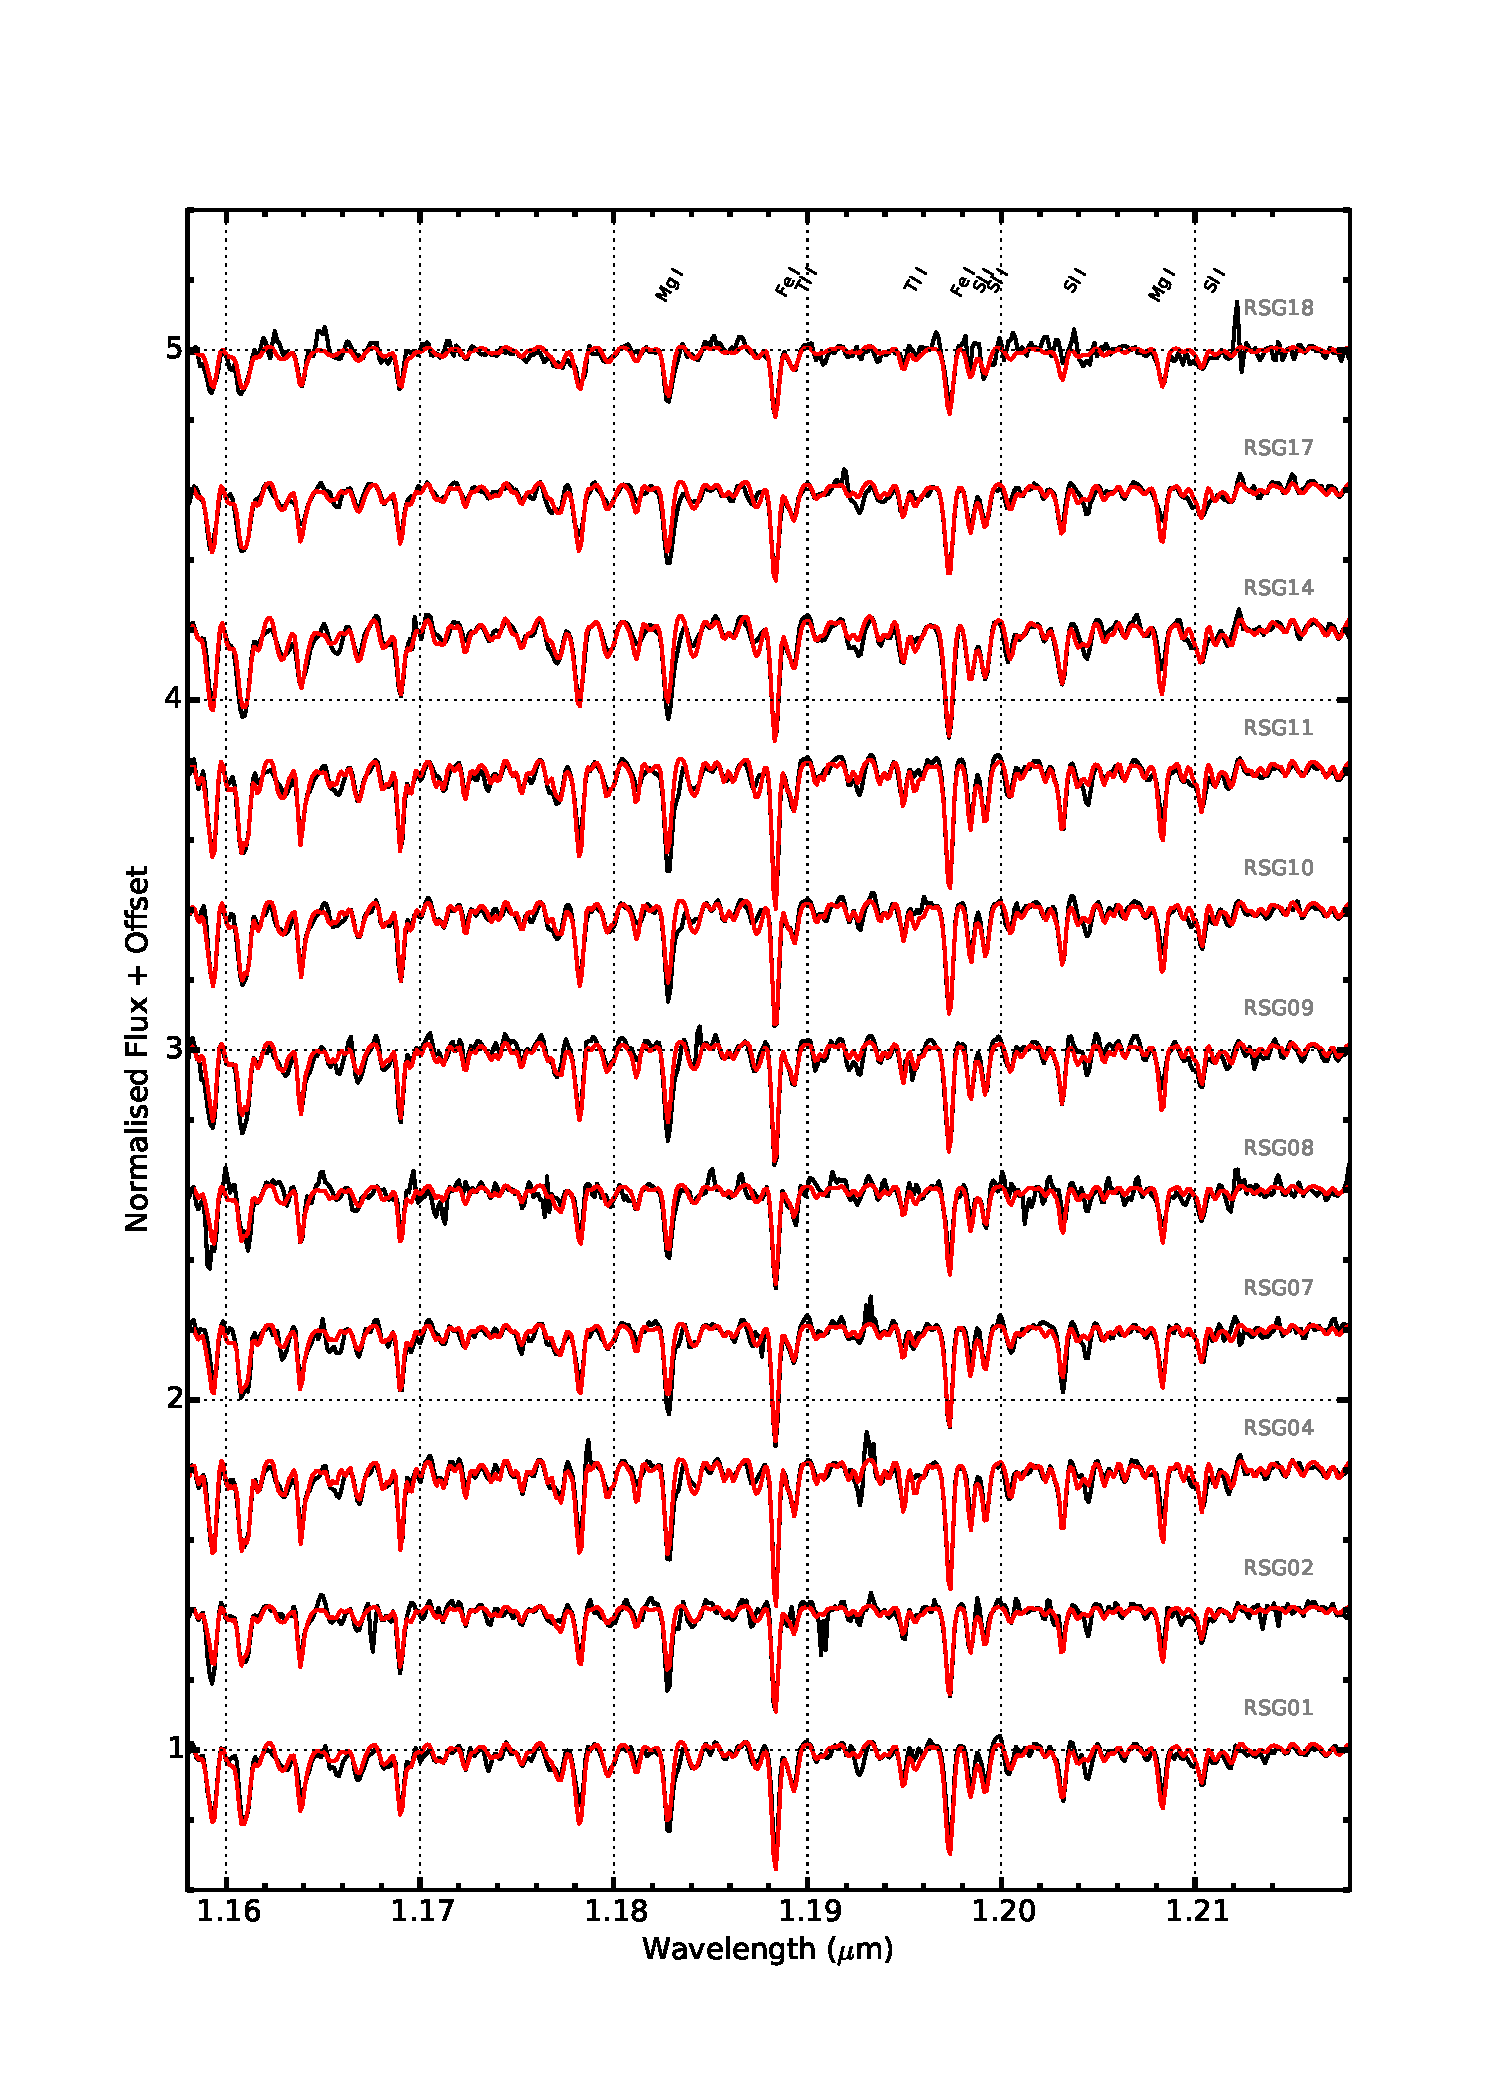
\includegraphics[width=\textwidth]{ngc6822/N6822_mod_fit.pdf}
\caption[Observed and best-fit model spectra]{
KMOS spectra of the NGC\,6822 RSGs and their associated best-fit model spectra
(black and red lines, respectively).
The lines used for the analysis from left-to-right by species are:
Fe\,\1$\lambda\lambda$1.188285,
1.197305,
Si\,\1$\lambda\lambda$1.198419,
1.199157,
1.203151,
1.210353,
Ti\,\1$\lambda\lambda$1.189289,
1.194954.
The two strong Mg\,\1 lines are also labelled, but are not used in the fits
(see Section~\ref{sec:results}).
         }
\label{fig:model_fits}
\end{center}
\end{figure*}


\begin{table*}
\scriptsize
 \caption[$c$-values]{
    Cross-correlation shift values and rescaling ($c$) values.
    }
 \label{c value}
 \begin{center}
  \begin{tabular}{lccccc}
   \hline
 Name  & \multicolumn{2}{c}{24 AT}  & \multicolumn{2}{c}{3 AT} \\
 &  Shift &  $c$  & Shift &  $c$\\
   \hline
   NGC6822-RSG01 &  0.143 & 0.112  &  0.051 & 0.130  \\ % N6822\_5  & J194443.81-144610.7
   NGC6822-RSG02 &  0.135 & 0.140  &  0.184 & 0.216  \\ % N6822\_8  & J194445.98-145102.4
   NGC6822-RSG03 &  0.115 & 0.104  &  0.036 & 0.112  \\ % N6822\_9  & J194447.13-144627.1
   NGC6822-RSG04 &  0.133 & 0.122  &  0.133 & 0.122  \\ % N6822\_12 & J194447.81-145052.5
   NGC6822-RSG05 &  0.054 & 0.198  & -0.017 & 0.206  \\ % N6822\_16 & J194450.54-144801.6
   NGC6822-RSG06 &  0.127 & 0.224  &  0.163 & 0.226  \\ % N6822\_21 & J194451.64-144858.0
   NGC6822-RSG07 & -0.048 & 0.148  &  0.052 & 0.092  \\ % N6822\_24 & J194453.46-144552.6
   NGC6822-RSG08 &  0.062 & 0.180  &  0.062 & 0.180  \\ % N6822\_25 & J194453.46-144540.1
   NGC6822-RSG09 &  0.077 & 0.060  &  0.012 & 0.090  \\ % N6822\_29 & J194454.46-144806.2
   NGC6822-RSG10 & -0.014 & 0.102  &  0.150 & 0.134  \\ % N6822\_30 & J194454.54-145127.1
   NGC6822-RSG11 &  0.067 & 0.134  &  0.060 & 0.110  \\ % N6822\_34 & J194455.70-145155.4
   NGC6822-RSG12 &  0.007 & 0.228  & -0.019 & 0.182  \\ % N6822\_36 & J194455.93-144719.6
   NGC6822-RSG13 & -0.329 & 0.290  & -0.310 & 0.342  \\ % N6822\_39 & J194456.86-144858.5
   NGC6822-RSG14 & -0.464 & 0.138  & -0.021 & 0.258  \\ % N6822\_40 & J194457.31-144920.2
   NGC6822-RSG15 & -0.324 & 0.206  & -0.585 & 0.250  \\ % N6822\_45 & J194459.14-144723.9
   NGC6822-RSG16 & -0.230 & 0.196  & -0.207 & 0.244  \\ % N6822\_47 & J194500.24-144758.9
   NGC6822-RSG17 & -0.192 & 0.160  & -0.192 & 0.160  \\ % N6822\_49 & J194500.53-144826.5
   NGC6822-RSG18 & -0.521 & 0.366  & -0.458 & 0.364  \\ % N6822\_55 & J194506.98-145031.1
   \hline
  \end{tabular}
 \end{center}
\end{table*}


% subsection ngc6822_telluric_correction (end)

\subsection{MOLECFIT} % (fold)
\label{sub:molecfit}

As an alternative to observing telluric standard stars, a new telluric correction package, {\sc molecfit}, allows one to calculate a telluric spectrum based on atmospheric modelling.
Briefly, the software uses a reference atmospheric profile to estimate the true profile for the time and location of the science observation.
This model is then used to create a telluric spectrum which can be used to correct the observations.

This software has been shown to work well, on a variety of VLT instruments
\citep{2015A&A...576A..77S} and has been rigorously tested using X-shooter spectra
\citep{2015A&A...576A..78K}.
However, the package has yet to be tested thoroughly on lower-resolution observations such as those from KMOS.
Our first tests appear encouraging, however, pending further characterisation of the KMOS data cubes
(e.g., small variations in spectral resolving power leading to sky residuals,
see Section~\ref{sub:sky_subtraction}),
I will investigate the potential of the {\sc molecfit} package with KMOS in the future.
% subsection molecfit (end)


\subsection{Stellar Radial Velocities} % (fold)
\label{sub:RVs}


Radial velocities for each target are listed in Table~\ref{tb:obs-params}.
The method used here to measure radial velocity values is consistent with that presented in \textbf{Chapter x.xx (i.e. as NGC\,2100)}.
Briefly, radial velocities are calculated using an iterative cross-correlation method.
Initially, the accuracy of the wavelength solution provided by the data reduction pipeline is checked against a spectrum of the Earth's telluric features.
Any offset is accounted for and the science spectrum is now assumed to be at ``rest'' wavelength.

Once the science spectra are at ``rest'' wavelength, the spectra are then cross-correlated again an appropriate synthetic RSG model using a large region where stellar features are known to dominate ($1.16-1.22\mu$m).
This initial guess is then improved on by selecting seven of the strongest spectral lines in this region and a radial velocity is calculated for each of these lines.
The final radial velocity is the mean of these seven strong lines where the error on the measurement is the standard deviation of the measurements normalised by the number of measurements
($err$~=~$\sigma_{rv}/N$).


Radial velocities estimates are shown as a function of distance to the centre of NGC\,6822 in Figure~\ref{fig:RvsRV}.
The average radial velocity for our targets is $-62\pm13$\,\kms,
in good agreement with the systemic radial velocity of the H\,\1 disk
\citep[$-57\pm2$\,\kms;][]{2004AJ....128...16K}.
Our radial velocities also agree with estimates for the two A-type supergiants from
\cite{2001ApJ...547..765V}.
This result confirms that our candidates are NGC\,6822 members.

\begin{figure}
 \centering
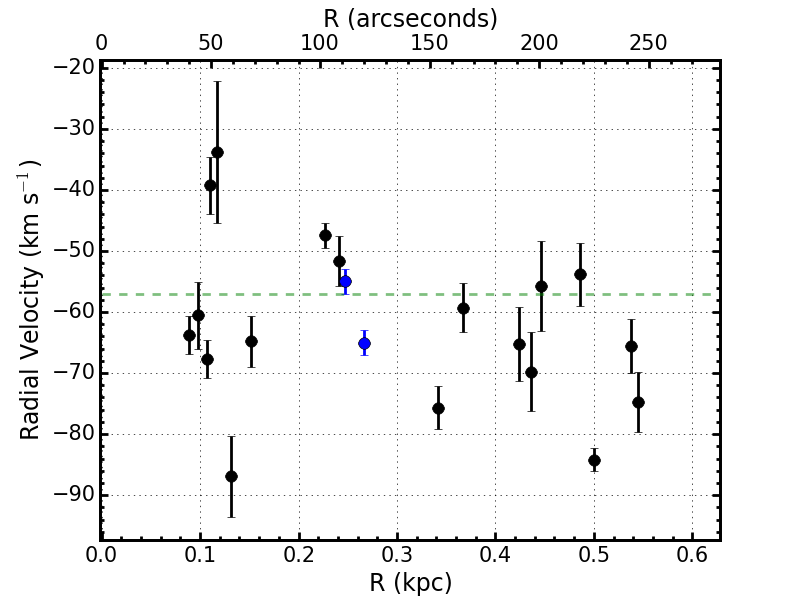
\includegraphics[width=0.65\textwidth]{ngc6822/N6822_RvsRV-v2}
\caption[Radial velocities shown against distance from galaxy centre]{
Radial velocities of targets shown against their distance from the galaxy centre.
The average radial velocity for the sample is $-62\pm13$\,\kms.
The green dashed line indicates H\,\1 systemic velocity
\protect\citep[$-57\pm2$\,\kms;][]{2004AJ....128...16K}.
The radial velocities of two A-type supergiants from
\protect\cite{2001ApJ...547..765V} are shown in blue.
        }
\label{fig:RvsRV}
\end{figure}

% subsection RVs (end)
% section data_reduction_and_analysis (end)


\section{Results} % (fold)
\label{sec:results}

Stellar parameters
(metallicity, effective temperature, surface gravity and microturbulence)
have been derived using the $J$-band analysis technique described by
\cite{2010MNRAS.407.1203D} and demonstrated by
\cite{2014ApJ...788...58G} and
\cite{2015ApJ...806...21D}.
To estimate physical parameters this technique uses a grid of synthetic spectra to fit observational data,
in which the models are degraded to the resolution of the observed spectra
(Table~\ref{tb:res}).
Model atmospheres were generated using the {\sc marcs} code
{\citep{2008A&A...486..951G}} where the range of parameters are defined in
Table~\ref{tb:mod_range}.
The precision of the models is increased by including departures from LTE in some of the strongest Fe, Ti and Si atomic lines
\citep{2012ApJ...751..156B,2013ApJ...764..115B}.
The two strong magnesium lines in our diagnostic spectral region are initially excluded from the analysis as these lines are known to be affected strongly by non-LTE effects
(see Figure~\ref{fig:model_fits}, where the two Mg\,\1 lines are systematically under- and over-estimated, respectively).
This is discussed further in Section~\ref{sub:with_mg}.


\begin{table}
\caption{
Model grid used for analysis.\label{tb:mod_range}
         }
\scriptsize
\begin{center}
\begin{tabular}{lccc}
 \hline
 \hline
  Model Parameter & Min. & Max. & Step size \\
 \hline
T$_{eff}$ (K)        & 3400 & 4000 & 100 \\
                     & 4000 & 4400 & 200 \\
$[$Z$]$ (dex)   & $-$1.50 & 1.00  & 0.25\\
log\,$g$ (cgs)  & $-$1.0\o & 1.0\o & 0.5\o \\
 $\xi$ (\kms)  & \pp1.0\o & 6.0\o & 1.0\o\\
 \hline
\end{tabular}
\end{center}
\end{table}

% subsection telluric_comparison (end)

\subsection{Telluric Comparison} % (fold)
\label{sub:telluric_comparison}

We used these Science Verification data to determine which of the two telluric standard methods is most appropriate for our analysis.
Table~\ref{tb:stellar-params} details the stellar parameters estimated for each target using both telluric methods and these parameters are compared in
Figure~\ref{fig:3vs24AT}.
The mean difference in the parameters between the two methods is
$<\Delta \xi>$~=~$-0.1 \pm 0.1$,
$\Delta [$Z$]$~=~$0.04\pm 0.07$,
$<\Delta$ log\,$g>$~=~$-0.06 \pm 0.12$ and
$<\Delta $T$_{\rm eff}>$~=~$-14 \pm 42$.
Therefore, for our analysis, there appears to be no significant difference between the two telluric approaches.


\begin{figure*}
 \centering
 \begin{center}$
  \centering
  \begin{array}{cc}
  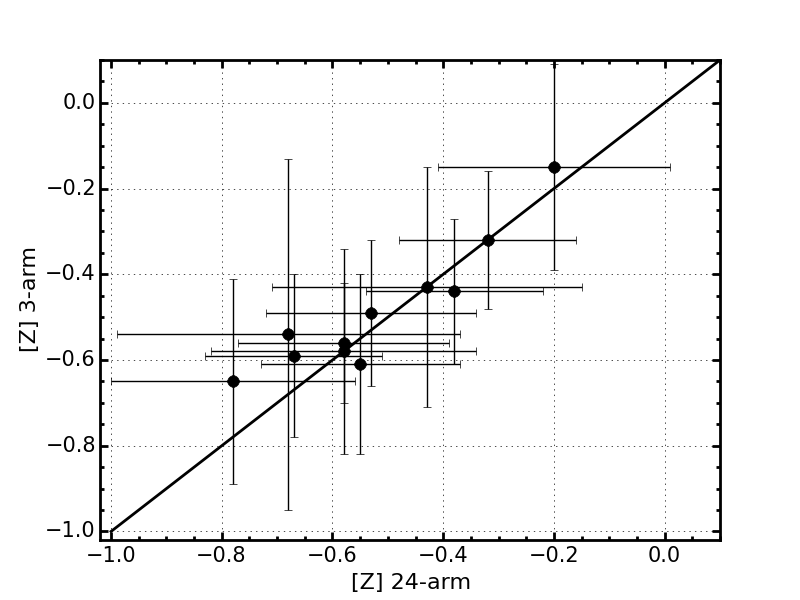
\includegraphics[width=0.5\textwidth]{ngc6822/N6822_24vs3AT_Z} &
  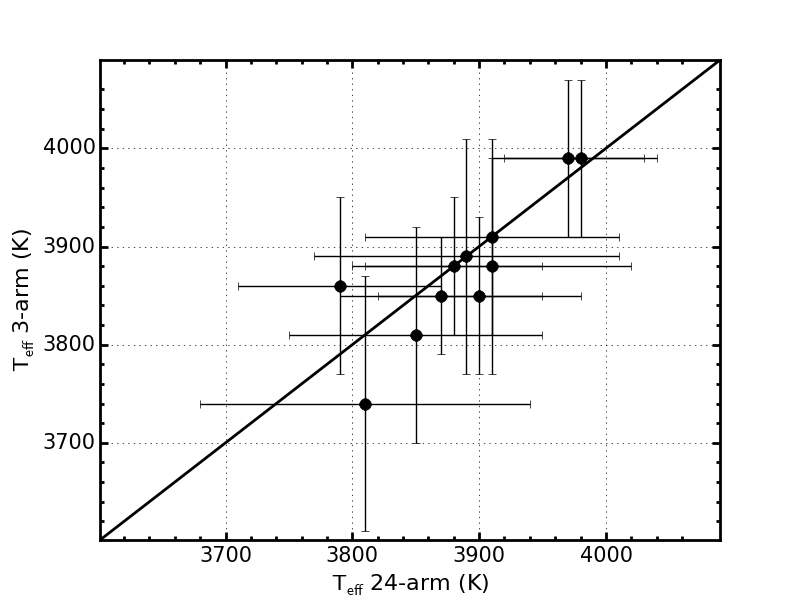
\includegraphics[width=0.5\textwidth]{ngc6822/N6822_24vs3AT_Teff} \\
  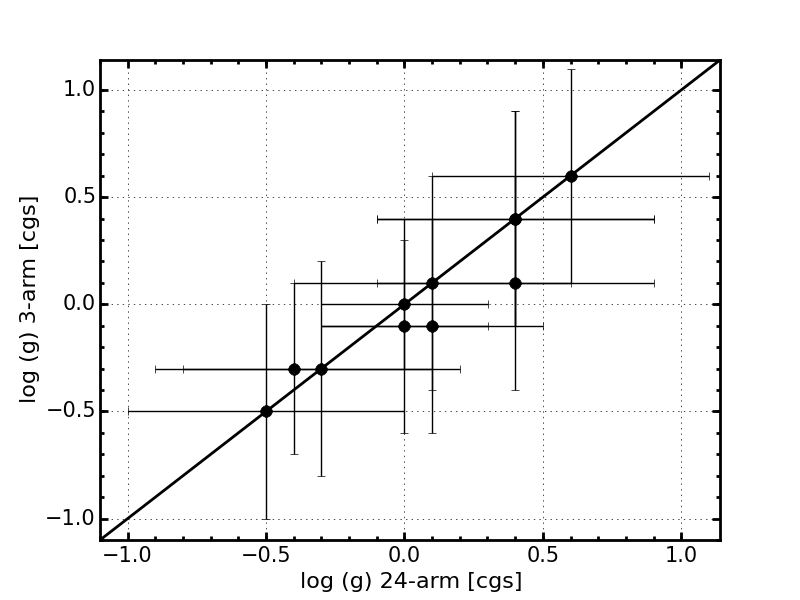
\includegraphics[width=0.5\textwidth]{ngc6822/N6822_24vs3AT_logg} &
  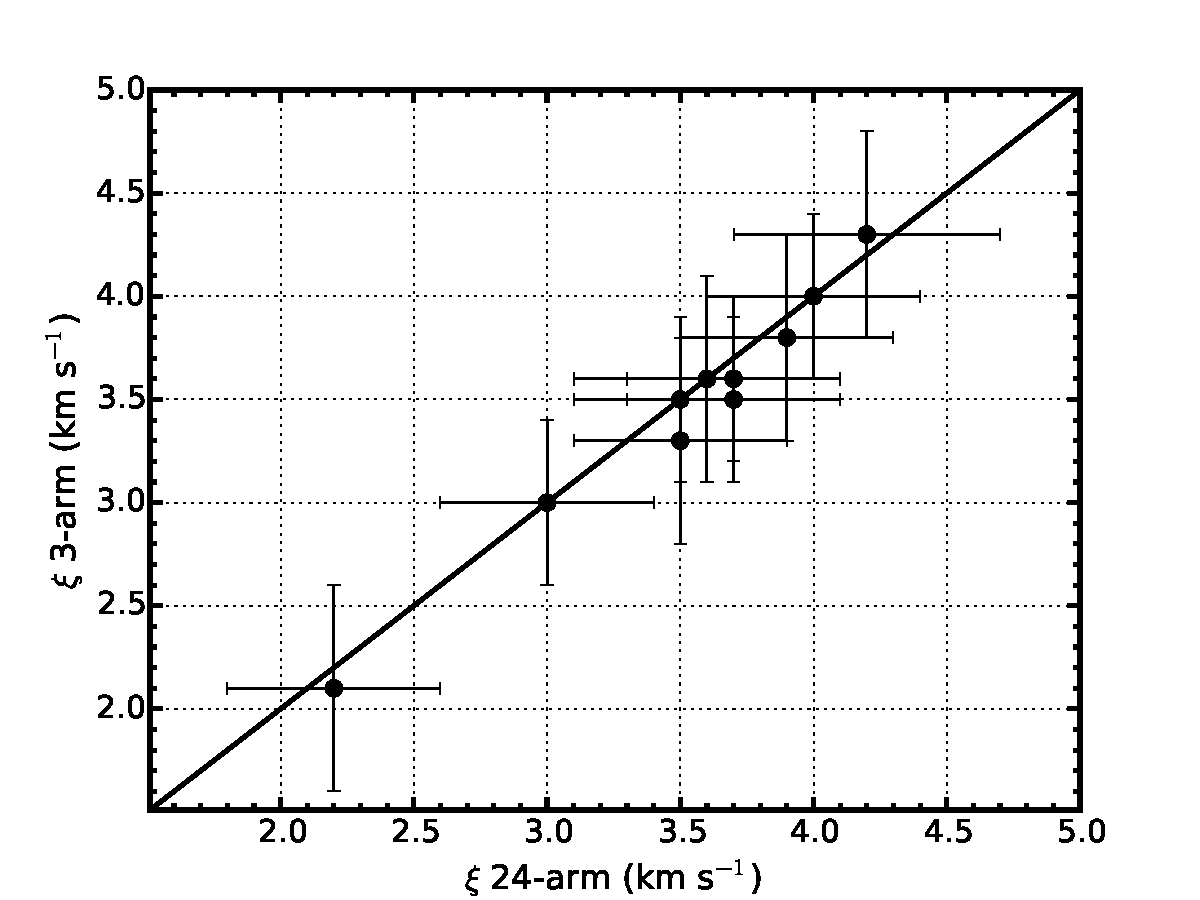
\includegraphics[width=0.5\textwidth]{ngc6822/N6822_24vs3AT_Xi} \\
  \end{array}$
 \end{center}
 \caption[Best-fit parameter comparison using the two telluric methods]{
            Comparison of the model parameters using the two different telluric methods.
            In each panel, the x-axis represents stellar parameters estimated using the 3 arm telluric
            method and the y-axis represents those estimated using the 24 arm telluric method.
            Top left: metallicity ([Z]), mean difference
            $<\Delta[$Z$]>$~=~$0.04 \pm 0.07$.
            Top right: effective temperature (T$_{\rm eff}$), mean difference
            $<\Delta $T$_{\rm eff}>$~=~$-14 \pm 42$.
            Bottom left: surface gravity (log\,$g$), mean difference
            $<\Delta$ log\,$g>$~=~$-0.06 \pm 0.12$.
            Bottom right: Microturbulence ($\xi$), mean difference
            $<\Delta \xi>$~=~$-0.1 \pm 0.1$.
            % Green dashed lines indicates linear best fits to the data.
            In all cases, the distributions are statistically consistent with a one-to-one ratio (black lines).
          }
 \label{fig:3vs24AT}
\end{figure*}


\begin{sidewaystable}
\begin{center}
\caption{
Fit parameters for reductions using the two different telluric methods.
\label{tb:stellar-params}
         }
\scriptsize
\begin{tabular}{lc cccc c cccc}
 \hline
 \hline
  Target  & IFU &  \multicolumn{4}{c}{24 Arm Telluric} & \multicolumn{4}{c}{3 Arm Telluric}\\
  \cline{3-6}  \cline{8-11}
 &  & T$_{eff}$ (K) & log\,$g$ & $\xi$ (\kms) & [Z] & & T$_{eff}$ (K) & log\,$g$ & $\xi$ (\kms) & [Z]\\
  \hline
NGC6822-RSG01 & 6 & 3790 $\pm$ 80\o & $-$0.0 $\pm$ 0.3 & 3.5 $\pm$ 0.4 & $-$0.55 $\pm$ 0.18 & & 3860 $\pm$ 90\o & $-$0.1 $\pm$ 0.5 &  3.5 $\pm$ 0.4 & $-$0.61 $\pm$ 0.21 \\
NGC6822-RSG02 & 11& 3850 $\pm$ 100  & \pp0.4 $\pm$ 0.5 & 3.5 $\pm$ 0.4 & $-$0.78 $\pm$ 0.22 & & 3810 $\pm$ 110  & \pp0.4 $\pm$ 0.5 &  3.3 $\pm$ 0.5 & $-$0.65 $\pm$ 0.24 \\
NGC6822-RSG04 & 12& 3880 $\pm$ 70\o & \pp0.0 $\pm$ 0.3 & 4.0 $\pm$ 0.4 & $-$0.32 $\pm$ 0.16 & & 3880 $\pm$ 70\o & \pp0.0 $\pm$ 0.3 &  4.0 $\pm$ 0.4 & $-$0.32 $\pm$ 0.16 \\
NGC6822-RSG07 & 2 & 3970 $\pm$ 60\o & \pp0.4 $\pm$ 0.5 & 3.9 $\pm$ 0.4 & $-$0.58 $\pm$ 0.19 & & 3990 $\pm$ 80\o & \pp0.1 $\pm$ 0.5 &  3.8 $\pm$ 0.5 & $-$0.56 $\pm$ 0.14 \\
NGC6822-RSG08 & 3 & 3910 $\pm$ 100  & \pp0.6 $\pm$ 0.5 & 3.0 $\pm$ 0.4 & $-$0.58 $\pm$ 0.24 & & 3910 $\pm$ 100  & \pp0.6 $\pm$ 0.5 &  3.0 $\pm$ 0.4 & $-$0.58 $\pm$ 0.24 \\
NGC6822-RSG09 & 4 & 3980 $\pm$ 60\o & \pp0.1 $\pm$ 0.4 & 3.7 $\pm$ 0.4 & $-$0.38 $\pm$ 0.16 & & 3990 $\pm$ 80\o & $-$0.1 $\pm$ 0.5 &  3.6 $\pm$ 0.4 & $-$0.44 $\pm$ 0.17 \\
NGC6822-RSG10 & 14& 3900 $\pm$ 80\o & $-$0.3 $\pm$ 0.5 & 3.7 $\pm$ 0.4 & $-$0.67 $\pm$ 0.16 & & 3850 $\pm$ 80\o & $-$0.3 $\pm$ 0.5 &  3.5 $\pm$ 0.4 & $-$0.59 $\pm$ 0.19 \\
NGC6822-RSG11 & 15& 3870 $\pm$ 80\o & $-$0.4 $\pm$ 0.5 & 4.2 $\pm$ 0.5 & $-$0.53 $\pm$ 0.19 & & 3850 $\pm$ 60\o & $-$0.3 $\pm$ 0.4 &  4.3 $\pm$ 0.5 & $-$0.49 $\pm$ 0.17 \\
NGC6822-RSG14 & 17& 3910 $\pm$ 110  & $-$0.5 $\pm$ 0.5 & 3.6 $\pm$ 0.5 & $-$0.20 $\pm$ 0.21 & & 3880 $\pm$ 110  & $-$0.5 $\pm$ 0.5 &  3.6 $\pm$ 0.5 & $-$0.15 $\pm$ 0.24 \\
NGC6822-RSG17 & 21& 3890 $\pm$ 120  & \pp0.1 $\pm$ 0.5 & 3.0 $\pm$ 0.4 & $-$0.43 $\pm$ 0.28 & & 3890 $\pm$ 120  & \pp0.1 $\pm$ 0.5 &  3.0 $\pm$ 0.4 & $-$0.43 $\pm$ 0.28 \\
NGC6822-RSG18 & 18& 3810 $\pm$ 130  & \pp0.4 $\pm$ 0.5 & 2.2 $\pm$ 0.4 & $-$0.68 $\pm$ 0.31 & & 3740 $\pm$ 130  & \pp0.4 $\pm$ 0.5 &  2.1 $\pm$ 0.5 & $-$0.54 $\pm$ 0.41 \\

% Stars not included in the sample:

% RSG9  & 5 & 4040 $\pm$ 130  & \pp0.8 $\pm$ 0.3 & 3.8 $\pm$ 0.6 & \pp0.14 $\pm$ 0.24 & 2500 & & 3990 $\pm$ 130  & \pp0.8 $\pm$ 0.3 &  3.8 $\pm$ 0.6 & \pp0.09 $\pm$ 0.24 & 2500 \\
% RSG16 & 7 & 4200 $\pm$ 50\o & \pp0.5 $\pm$ 0.4 & 2.3 $\pm$ 0.3 & $-$0.51 $\pm$ 0.16 & 4400 & & 4230 $\pm$ 100  & \pp0.5 $\pm$ 0.2 &  2.4 $\pm$ 0.3 & $-$0.54 $\pm$ 0.15 & 4400 \\
% RSG21 & 10& 3780 $\pm$ 110  & \pp0.4 $\pm$ 0.5 & 2.3 $\pm$ 0.4 & $-$0.55 $\pm$ 0.32 & 3800 & & 3790 $\pm$ 90\o & \pp0.5 $\pm$ 0.5 &  2.2 $\pm$ 0.4 & $-$0.46 $\pm$ 0.33 & 3800 \\
% RSG36 & 1 & 3840 $\pm$ 120  & \pp0.6 $\pm$ 0.5 & 3.0 $\pm$ 0.4 & $-$0.52 $\pm$ 0.26 & 3300 & & 3930 $\pm$ 100  & \pp0.6 $\pm$ 0.4 &  2.9 $\pm$ 0.4 & $-$0.39 $\pm$ 0.25 & 3300 \\
% RSG39 & 19& 3870 $\pm$ 130  & \pp0.5 $\pm$ 0.5 & 2.4 $\pm$ 0.5 & $-$0.73 $\pm$ 0.26 & 3000 & & 3800 $\pm$ 120  & \pp0.4 $\pm$ 0.5 &  2.1 $\pm$ 0.5 & $-$0.58 $\pm$ 0.33 & 3000 \\
% RSG45 & 24& 4220 $\pm$ 120  & \pp0.6 $\pm$ 0.5 & 2.9 $\pm$ 0.4 & $-$0.24 $\pm$ 0.20 & 3200 & & 4290 $\pm$ 120  & \pp0.6 $\pm$ 0.5 &  3.0 $\pm$ 0.5 & $-$0.27 $\pm$ 0.22 & 3200 \\
% RSG47 & 22& 3980 $\pm$ 90\o & \pp0.4 $\pm$ 0.4 & 3.2 $\pm$ 0.4 & $-$0.57 $\pm$ 0.23 & 2700 & & 3950 $\pm$ 100  & \pp0.4 $\pm$ 0.4 &  3.3 $\pm$ 0.4 & $-$0.64 $\pm$ 0.24 & 2700 \\

  \hline
  \end{tabular}
  \end{center}
\end{sidewaystable}

\subsection{The Introduction of Magnesium} % (fold)
\label{sub:with_mg}

Since the publication of~\citet[][where the results from this chapter are published]{2015ApJ...803...14P}, non-LTE corrections have been calculated by~\cite{2015ApJ...804..113B}.
Using these results, the model grids have now been updated to include the corrections for non-LTE for the Mg\,\1 lines.
As an additional calibration to these corrections~\citep[to the extensive testing in][]{2015ApJ...804..113B} I have used the updated model grids to re-analyse the NGC\,6822 KMOS spectra.
This allows a direct comparison between results including and excluding the Mg\,\1 lines.


% By implementing these corrections to the model grid stellar parameters can now be calculated including the Mg\,\1 lines.

Figure~\ref{fig:24ATvs24Mg} displays the stellar parameters estimated including and excluding the two Mg\,\1 lines.
This figure shows that there exists no significant difference between the results when the Mg\,\1 lines are included.
Table~\ref{tb:stellar-params-Mg} details the parameters.

For the remainder of this chapter we adopt the updated stellar parameters including the non-LTE effects of Magnesium.

\begin{figure*}
 \centering
 \begin{center}
  \centering
  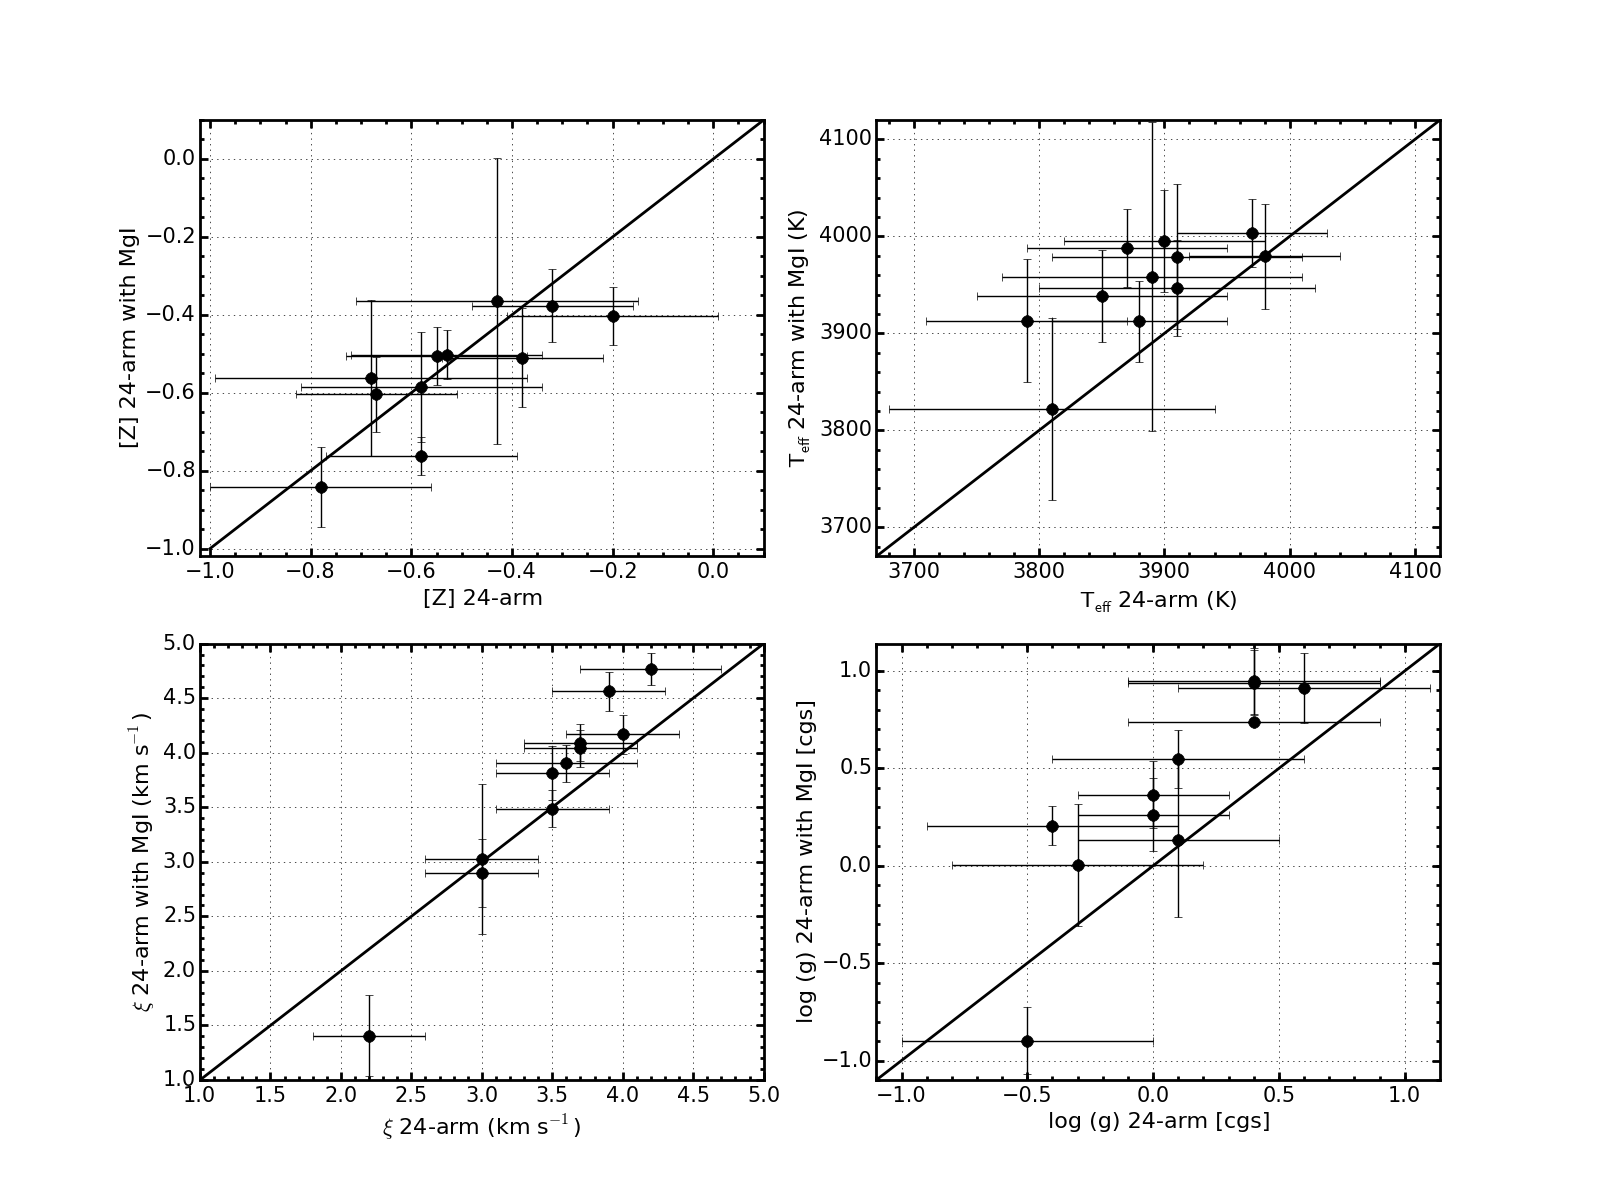
\includegraphics[width=\textwidth]{ngc6822/N6822-Mg-compare}
 \end{center}
 \caption[Best-fit parameter comparison using including and excluding Mg\,\1]{
            Comparison of the model parameters including and excluding Mg\,\1 lines.
            In each panel, the x-axis represents stellar parameters estimated excluding the Mg\,\1 lines
            and the y-axis represents those estimated including the Mg\,\1 lines.
            Top left: metallicity ([Z]), mean difference
            $<\Delta[$Z$]>$~=~0.03$\pm$0.10.
            Top right: effective temperature (T$_{\rm eff}$), mean difference
            $<\Delta$T$_{\rm eff}>$~=~$-$61$\pm$39.
            Bottom left: surface gravity (log\,$g$), mean difference
            $<\Delta$log\,$g>$~=~$-$0.11$\pm$0.37.
            Bottom right: Microturbulence ($\xi$), mean difference
            $<\Delta \xi>$~=~$-$0.17$\pm$0.38.
            % Green dashed lines indicates linear best fits to the data.
            In all cases, the distributions are statistically consistent with a one-to-one ratio (black lines).
          }
 \label{fig:24ATvs24Mg}
\end{figure*}


\begin{sidewaystable}
\begin{center}
\caption{
Fit parameters including and excluding Mg\,\1 lines.
\label{tb:stellar-params-Mg}
         }
\scriptsize
\begin{tabular}{lc cccc c cccc}
 \hline
 \hline
  Target  & IFU &  \multicolumn{4}{c}{24 Arm Telluric with Mg\,\1} & \multicolumn{4}{c}{24 Arm Telluric with Mg\,\1}\\
  \cline{3-6}  \cline{8-11}
 &  & $\xi$ (\kms) & [Z] & log\,$g$ & T$_{eff}$ (K) & & $\xi$ (\kms) & [Z] & log\,$g$ & T$_{eff}$ (K)\\
  \hline
NGC6822-RSG01 & 6 & 3.5$\pm$0.4 & $-$0.55$\pm$0.18 & $-$0.0$\pm$0.3 & 3790$\pm$80\o & & 3.5$\pm$0.2 & $-$0.51$\pm$0.07 & \pp0.26$\pm$0.19 & 3910$\pm$60\o\\
NGC6822-RSG02 & 11& 3.5$\pm$0.4 & $-$0.78$\pm$0.22 & \pp0.4$\pm$0.5 & 3850$\pm$100  & & 3.8$\pm$0.2 & $-$0.84$\pm$0.10 & \pp0.94$\pm$0.17 & 3940$\pm$50\o\\
NGC6822-RSG04 & 12& 4.0$\pm$0.4 & $-$0.32$\pm$0.16 & \pp0.0$\pm$0.3 & 3880$\pm$70\o & & 4.2$\pm$0.2 & $-$0.38$\pm$0.09 & \pp0.36$\pm$0.17 & 3910$\pm$40\o\\
NGC6822-RSG07 & 2 & 3.9$\pm$0.4 & $-$0.58$\pm$0.19 & \pp0.4$\pm$0.5 & 3970$\pm$60\o & & 4.6$\pm$0.2 & $-$0.76$\pm$0.05 & \pp0.74$\pm$0.00 & 4000$\pm$40\o\\
NGC6822-RSG08 & 3 & 3.0$\pm$0.4 & $-$0.58$\pm$0.24 & \pp0.6$\pm$0.5 & 3910$\pm$100  & & 2.9$\pm$0.3 & $-$0.59$\pm$0.14 & \pp0.91$\pm$0.18 & 3980$\pm$80\o\\
NGC6822-RSG09 & 4 & 3.7$\pm$0.4 & $-$0.38$\pm$0.16 & \pp0.1$\pm$0.4 & 3980$\pm$60\o & & 4.1$\pm$0.2 & $-$0.51$\pm$0.13 & \pp0.13$\pm$0.40 & 3980$\pm$50\o\\
NGC6822-RSG10 & 14& 3.7$\pm$0.4 & $-$0.67$\pm$0.16 & $-$0.3$\pm$0.5 & 3900$\pm$80\o & & 4.0$\pm$0.2 & $-$0.60$\pm$0.10 & \pp0.00$\pm$0.31 & 4000$\pm$50\o\\
NGC6822-RSG11 & 15& 4.2$\pm$0.5 & $-$0.53$\pm$0.19 & $-$0.4$\pm$0.5 & 3870$\pm$80\o & & 4.8$\pm$0.1 & $-$0.50$\pm$0.06 & \pp0.20$\pm$0.10 & 3990$\pm$40\o\\
NGC6822-RSG14 & 17& 3.6$\pm$0.5 & $-$0.20$\pm$0.21 & $-$0.5$\pm$0.5 & 3910$\pm$110  & & 3.9$\pm$0.2 & $-$0.40$\pm$0.07 & $-$0.90$\pm$0.17 & 3950$\pm$50\o\\
NGC6822-RSG17 & 21& 3.0$\pm$0.4 & $-$0.43$\pm$0.28 & \pp0.1$\pm$0.5 & 3890$\pm$120  & & 3.0$\pm$0.7 & $-$0.36$\pm$0.37 & \pp0.55$\pm$0.15 & 3960$\pm$160\\
NGC6822-RSG18 & 18& 2.2$\pm$0.4 & $-$0.68$\pm$0.31 & \pp0.4$\pm$0.5 & 3810$\pm$130  & & 1.4$\pm$0.4 & $-$0.56$\pm$0.20 & \pp0.95$\pm$0.17 & 3820$\pm$90\o\\

% Stars not included in the sample:

% RSG9  & 5 & 4040 $\pm$ 130  & \pp0.8 $\pm$ 0.3 & 3.8 $\pm$ 0.6 & \pp0.14 $\pm$ 0.24 & 2500 & & 3990 $\pm$ 130  & \pp0.8 $\pm$ 0.3 &  3.8 $\pm$ 0.6 & \pp0.09 $\pm$ 0.24 & 2500 \\
% RSG16 & 7 & 4200 $\pm$ 50\o & \pp0.5 $\pm$ 0.4 & 2.3 $\pm$ 0.3 & $-$0.51 $\pm$ 0.16 & 4400 & & 4230 $\pm$ 100  & \pp0.5 $\pm$ 0.2 &  2.4 $\pm$ 0.3 & $-$0.54 $\pm$ 0.15 & 4400 \\
% RSG21 & 10& 3780 $\pm$ 110  & \pp0.4 $\pm$ 0.5 & 2.3 $\pm$ 0.4 & $-$0.55 $\pm$ 0.32 & 3800 & & 3790 $\pm$ 90\o & \pp0.5 $\pm$ 0.5 &  2.2 $\pm$ 0.4 & $-$0.46 $\pm$ 0.33 & 3800 \\
% RSG36 & 1 & 3840 $\pm$ 120  & \pp0.6 $\pm$ 0.5 & 3.0 $\pm$ 0.4 & $-$0.52 $\pm$ 0.26 & 3300 & & 3930 $\pm$ 100  & \pp0.6 $\pm$ 0.4 &  2.9 $\pm$ 0.4 & $-$0.39 $\pm$ 0.25 & 3300 \\
% RSG39 & 19& 3870 $\pm$ 130  & \pp0.5 $\pm$ 0.5 & 2.4 $\pm$ 0.5 & $-$0.73 $\pm$ 0.26 & 3000 & & 3800 $\pm$ 120  & \pp0.4 $\pm$ 0.5 &  2.1 $\pm$ 0.5 & $-$0.58 $\pm$ 0.33 & 3000 \\
% RSG45 & 24& 4220 $\pm$ 120  & \pp0.6 $\pm$ 0.5 & 2.9 $\pm$ 0.4 & $-$0.24 $\pm$ 0.20 & 3200 & & 4290 $\pm$ 120  & \pp0.6 $\pm$ 0.5 &  3.0 $\pm$ 0.5 & $-$0.27 $\pm$ 0.22 & 3200 \\
% RSG47 & 22& 3980 $\pm$ 90\o & \pp0.4 $\pm$ 0.4 & 3.2 $\pm$ 0.4 & $-$0.57 $\pm$ 0.23 & 2700 & & 3950 $\pm$ 100  & \pp0.4 $\pm$ 0.4 &  3.3 $\pm$ 0.4 & $-$0.64 $\pm$ 0.24 & 2700 \\

  \hline
  \end{tabular}
  \end{center}
\end{sidewaystable}


% subsection the_introduction_of_magnesium (end)

\subsection{Stellar Parameters and Metallicity} % (fold)
\label{sub:stellar_parameters_and_metallicity}

Table~\ref{tb:stellar-params-Mg} summarises the estimated stellar parameters.
For the remainder of this chapter, when discussing stellar parameters,
we adopt those estimated using the 24 arm telluric method including the Mg\,\1 lines.
(i.e. the results in the left-hand part of Table~\ref{tb:stellar-params-Mg}.)
The average metallicity for our sample of 11 RSGs in NGC\,6822 is
$\bar{Z}$~=~$-0.55\pm0.13$.
This result is in good agreement with the average metallicity estimated in
\citet[][see also Figure~\ref{fig:ZvsR}]{2015ApJ...803...14P}.
In addition the results presented here are also in good agreement with results using BSGs
\citep[BSGs;][]{1999A&A...352L..40M,2001ApJ...547..765V}.

A direct comparison with metallicities from BSGs is legitimate as the method used in the present analysis yield a global metallicity ([Z]) which
closely resembles the Fe/H ratio estimated in
\cite{2001ApJ...547..765V}.
While our [Z] measurements are also affected by Si and Ti,
we assume [Z]~=~[Fe/H] for the purposes of our discussion.
Likewise, we can compare oxygen abundances (relative to solar) obtained from H\,\2 regions as a proxy for [Z] by
introducing the solar oxygen abundance
{12+log\,(O/H)}$_{\odot}$~=~8.69
\citep{2009ARA&A..47..481A} through the relation
[Z]~=~$12 + $log\,(O/H)$ - 8.69$.
This implicitly assumes that the $\alpha$/Fe ratio remains Solar in different environments.

As outlined in \textbf{Chapter x.x} the RSG and BSG stages are different evolutionary phases within the life cycle of a massive star,
while H\,\2 regions are the birth clouds which give rise to the youngest stellar population.
As the lifetimes of RSGs and BSGs are $<50$Myr,
their metallicity estimates are also expected to be representative of their birth clouds.

To investigate the spatial distribution of chemical abundances in NGC\,6822,
in Figure~\ref{fig:ZvsR}
we show the metallicities of our RSGs as a function of radial distance from the centre of the galaxy,
as well as the results from
\cite{2001ApJ...547..765V} and the indicative estimates from
\cite{1999A&A...352L..40M}.


A least-squares fit to the results from~\cite{2015ApJ...803...14P} reveals a low-significance abundance gradient within the central 1\,kpc of NGC\,6822 of $-0.5\pm0.4\,dex\,$kpc$^{-1}$.
In addition, the extrapolated central metallicity from the fit (i.e. at R~=~0) of [Z]~=~$-0.30\pm0.15\,dex$ remains consistent with the average metallicity assuming no gradient.
However, using the updated stellar parameters the data appears consistent with no gradient ($-0.12\pm0.19\,dex\,$kpc$^{-1}$) even though statistically this is a poorer fit to the data.


\begin{figure}
 \centering
 \begin{center}$
  \centering
  \begin{array}{cc}
  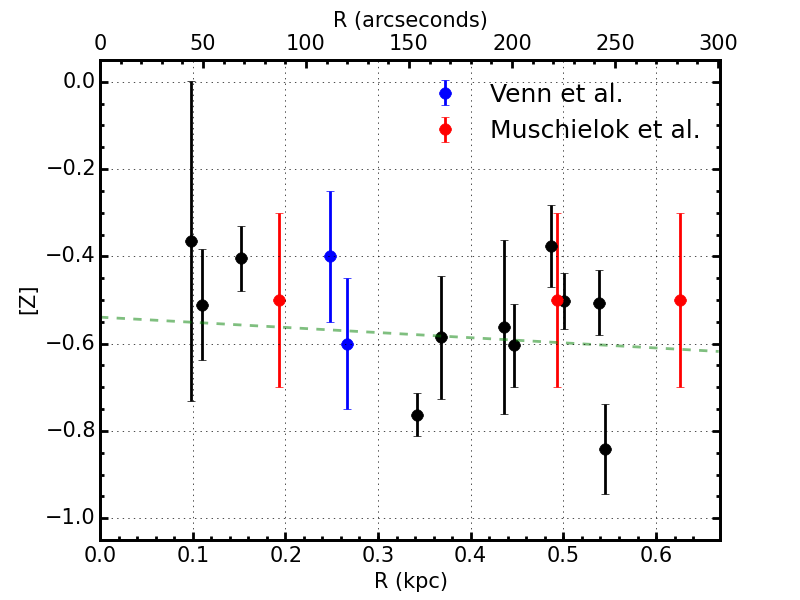
\includegraphics[width=0.5\textwidth]{ngc6822/N6822_ZvsR-thesis} &
  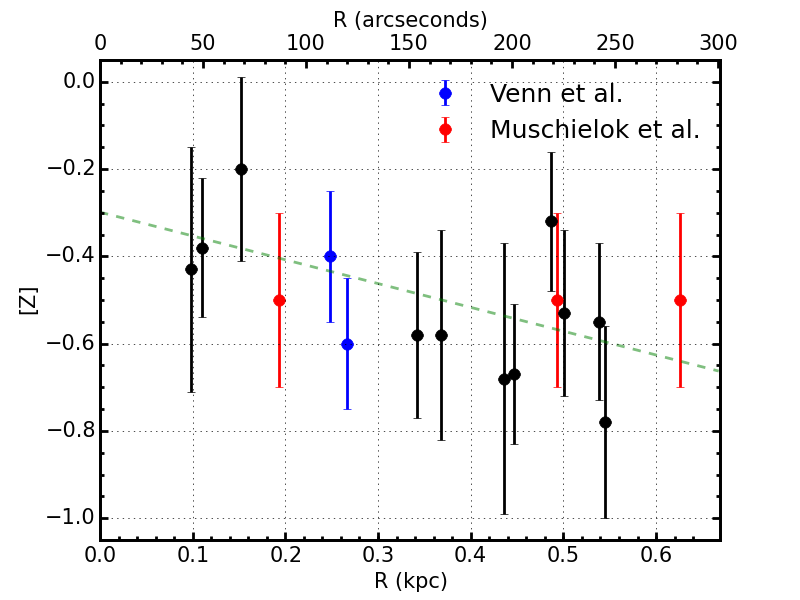
\includegraphics[width=0.5\textwidth]{ngc6822/N6822_ZvsR_BSG} \\
  \end{array}$
 \end{center}
\caption[Metallicities shown against distance from the galaxy centre]{
Estimated metallicities for 11 RSGs in NGC\,6822 shown against their distance from the galaxy centre.
The left panel shows the metallicities estimated including Mg\,\1 lines whereas the right hand panel shows metallicities excluding Mg\,\1.
Blue and red points show BSG results from
\cite{2001ApJ...547..765V} and
\cite{1999A&A...352L..40M} respectively.
The average metallicity is consistent between the two samples and the average including Mg\,\1 is adopted at
$\bar{\rm Z}$~=~$-0.55\pm0.13$.
A least-squares fit to the results excluding Mg\,\1 (right panel) reveals a low-significance abundance gradient
(see text for details).
For comparison,
R$_{25}$~=~460\,arcseconds
\protect\citep[=~1.03\,kpc;][]{2012AJ....144....4M}.
\label{fig:ZvsR}
}
\end{figure}

Figure~\ref{fig:6822HRD} shows the location of our sample in the Hertzsprung-Russell (H-R) diagram.
Bolometric corrections were computed using the calibration in
\cite{2013ApJ...767....3D}.
This figure shows that the temperatures estimated using the $J$-band method are systematically cooler than the end of the evolutionary models (which terminate at the end of the carbon-burning phase for massive stars) for
Z~=~0.002 from
\cite{2013A&A...558A.103G}.
This result is discussed in Section~\ref{sub:temperatures_of_rsgs}.


\begin{figure}
 \centering
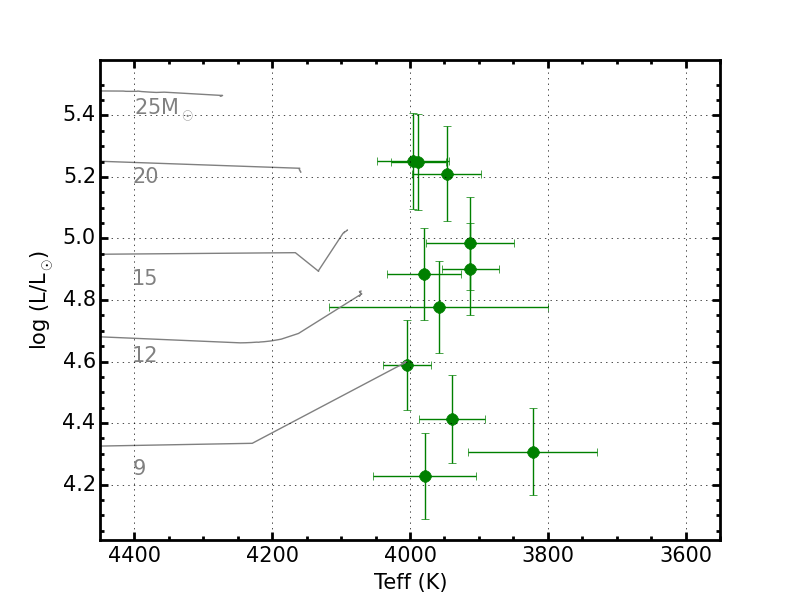
\includegraphics[width=0.65\textwidth]{ngc6822/N6822_HRD_thesis}
\caption[H-R diagram for NGC\,6822]{
H-R diagram for the 11 RSGs in NGC\,6822.
Evolutionary tracks including rotation
($v/v_{c}$~=~0.4) for SMC-like metallicity (Z~=~0.002)
are shown in grey, along with their zero-age mass
\protect\citep{2013A&A...558A.103G}.
Bolometric corrections are computed using the calibration in
\protect\cite{2013ApJ...767....3D}.
We note that compared to the evolutionary tracks,
the observed temperatures of NGC\,6822 RSGs are systematically cooler.
This is discussed in Section~\ref{sub:temperatures_of_rsgs}.
}
\label{fig:6822HRD}
\end{figure}

% subsection stellar_parameters (end)
% section results (end)


\section{Discussion} % (fold)
\label{sec:discussion}

\subsection{Metallicity Measurements} % (fold)
\label{sub:metallicity_measurements}

The average metallicity for the sample is $\bar{\rm Z}$~=~$-$0.55$\pm$0.13,
which agrees well with the results estimated from BSGs
\citep{1999A&A...352L..40M,2001ApJ...547..765V,2002PhDT.........3P} and H\,\2 regions
\citep{2006ApJ...642..813L}.
These results are consistent with no metallicity gradient within NGC\,6822.


Using the data from \citep[][i.e excluding Mg\,\1]{2015ApJ...803...14P} there exists a low-significance metallicity gradient within the central 1\,kpc of NGC\,6822
($-0.5\pm0.4\,dex\,$kpc$^{-1}$ with a $\chi^{2}_{red}$~=~1.16; see Figure~\ref{fig:ZvsR}).
The gradient estimated is consistent with the trend reported in
\cite{2001ApJ...547..765V}
from their results for the two BSGs which these authors compared with H\,\2 regions
\citep{1980MNRAS.193..219P} and two planetary nebulae
\citep{1995ApJ...445..642R} at larger galactocentric distances.
This result is also consistent with the gradient estimated from a sample of 49 local star-forming galaxies
\citep{2015MNRAS.448.2030H}.
Including the results for BSGs from
\cite{2001ApJ...547..765V}
in the analysis,
gives a consistent gradient
($-0.48\pm 0.33\,dex$\,kpc$^{-1}$)
with an improved
$\chi^{2}_{red}$~=~1.06.
Results from
\cite{1999A&A...352L..40M} are not included in the fit as these measurements were qualitative estimates of metallicity.



In contrast,
\cite{2006ApJ...642..813L} used the oxygen abundances from 19 H\,\2
regions and found no clear evidence for a metallicity gradient.
Using a subset of the highest quality H\,\2
region data available, these authors found a gradient of
$-0.16\pm0.05dex\,$kpc$^{-1}$.
Including these results into our analysis degrades the fit and changes the estimated gradient significantly
($-0.18\pm0.05dex\,$kpc$^{-1}$; $\chi^{2}_{red}$~=~1.78).
However, when this data is combined with the RSG data including the Mg\,\1 lines, a significant gradient is measured
($-0.13\pm0.04dex\,$kpc$^{-1}$; $\chi^{2}_{red}$~=~2.91).
At this point it is not clear whether the indication of a gradient obtained from the RSGs and BSGs is an artefact of the small sample size,
or indicates a difference with respect to the H\,\2 region study.


There have been a number of studies of the metallicity of the older stellar population in NGC\,6822.
From spectroscopy of red giant branch (RGB) stars,
\cite{2001MNRAS.327..918T} found a mean metallicity of [Fe/H]~=~$-0.9$
with a reasonably large spread (see their Figure 19).
More recently,
\cite{2012A&A...540A.135S} derived metallicities using a population of AGB stars within the central 4\,kpc of NGC\,6822.
They found an average metallicity of [Fe/H]~=~$-1.29\pm0.07\,dex$.
Likewise,
\cite{2013ApJ...779..102K}
used spectra of red giant stars within the central 2\,kpc and found an average metallicity of
[Fe/H]~=~$-1.05\pm0.49\,dex$.
We note that none of these studies found any compelling evidence for spatial variations in the stellar metallicities,
which is not surprising given that, in disc galaxies, radial migration is thought to smooth out any abundance gradients over time.
The stellar populations used for these studies are known to be significantly older than our sample,
therefore, owing to the chemical evolution in the time since the birth of the older populations,
we expect the measured metallicities to be significantly lower.

The low metallicity of the young stellar population and the interstellar medium (ISM) in NGC\,6822 can be understood as a consequence of the fact that it is a relatively gas-rich galaxy with a mass
M$_{HI}$~=~1.45$\times$10$^{8}$\,M$_{\odot}$
\citep{2004AJ....128...16K} and a total stellar mass of ranging from
M$_{*}$~=~$0.83$~-~$1.70\times$10$^{8}$ M$_{\odot}$
\citep{2008MNRAS.390.1453W,2013ApJ...779..102K,2014ApJ...789..147W}.

The simple closed-box chemical-evolution model relates the metallicity mass fraction $Z(t)$ at any time to the ratio of stellar to gas mass $M_{*}\over M_{g}$ through

\begin{equation}\label{closed-box}
Z(t) = {y \over 1-R } \ln \left[ 1 + {M_{*}(t)\over M_{g}(t)}  \right],
\end{equation}

\noindent where $y$ is the fraction of metals per stellar mass produced through stellar nucleosynthesis
(the so-called yield) and $R$ is the fraction of stellar mass returned to the ISM through stellar mass-loss.

According to
\citet{2015MNRAS.450..342K}, the ratio $y/(1-R)$ can be empirically determined from the fact that the metallicity of the young stellar population in the solar neighbourhood is solar, with a mass fraction Z$_{\odot}$~=~0.014
\citep{2012A&A...539A.143N}.
With a stellar-to-gas mass column density of 4.48 in the solar neighbourhood
\citep{2003ApJ...587..278W,2013ApJ...779..115B}
one then obtains $y/(1-R)$~=~0.0082~=~0.59Z\,$_{\odot}$ with an uncertainty of 15 percent dominated by the 0.05\,$dex$ uncertainty of the metallicity determination of the young population.

Accounting for the presence of helium and metals in the neutral interstellar gas we can turn the observed HI mass in NGC\,6822 into a gas mass via
M$_{g}$~=~1.36\,M$_{HI}$ and use the simple closed-box model to predict a metallicity of
[Z]~=~$-0.44$~-~$-0.69$,
in good agreement with our value obtained from RSG spectroscopy.

As discussed above, the older stellar population of AGB stars has a metallicity roughly 0.8\,$dex$ lower than the RSGs.
In the framework of the simple closed-box model this would correspond to a period in time where the ratio of stellar to gas mass was $\sim$~0.1
(much lower than the present value of 0.42-0.86).
The present star-formation rate of NGC\,6822 is $\sim$~0.02\,M$_{\odot}$yr$^{-1}$
\citep{2010A&A...512A..68G,2011ApJ...730...88E}.
At such a high level of star formation it would have taken five Gyr to produce the presently observed stellar mass and to arrive from the average metallicity of the AGB stars to that of the young stellar population
(of course, again relying on the simple closed-box model).
Evidence suggests that the star-formation rate was substantially lower in the past
\citep{2011ApJ...730...88E,2014ApJ...789..147W},
therefore, the build up of the observed stellar mass would have taken correspondingly longer.


Given the irregularities present in the stellar and gaseous morphology of NGC\,6822, this galaxy may not be a good example of a closed-box system, however it is remarkable that the closed-box model reproduces the observed metallicity so closely.

% subsection abundance_measurements (end)

\subsection{Temperatures of RSGs} % (fold)
\label{sub:temperatures_of_rsgs}

Effective temperatures have been estimated for 11 RSGs from our observed sample in NGC\,6822.
To date, this represents the fourth data set used to estimate stellar parameters in this way and the first with KMOS.
The previous three data sets which have been analysed are those of 11 RSGs in PerOB1,
a Galactic star cluster
\citep{2014ApJ...788...58G}, nine RSGs in the LMC and 10 RSGs in the SMC
\citep[both from][]{2015ApJ...806...21D}.
These results range from Z~=~Z$_{\odot}$ in PerOB1 to Z~=~0.3Z$_{\odot}$ in the SMC, around 0.5\,$dex$ in metallicity.

We compare the effective temperatures estimated in this study to those of the previous results in different environments.
Their distribution is shown as a function of metallicity in Figure~\ref{fig:TvsZ}.
Additionally, Figure~\ref{fig:HRD} shows the H-R diagram for the four sets of results.
Bolometric corrections to calculate the luminosities for each sample were computed using the calibration in
\cite{2013ApJ...767....3D}.


\begin{figure}
 \centering
\includegraphics[width=0.65\textwidth]{ngc6822/N6822_TeffvsZ-thesis}
\caption[Effective temperature as a function of metallicity in different environments]{
Effective temperatures as a function of metallicity for four different data sets using the $J$-band analysis technique.
There appears to be no significant variation in the temperatures of RSGs over a range of 0.55 dex.
These results are compiled from the LMC, SMC
\protect\citep[blue and red points respectively;][]{2015ApJ...806...21D}, PerOB1
\protect\citep[a Galactic RSG cluster; cyan;][]{2014ApJ...788...58G} and NGC\,6822 (green).
Mean values for each data set are shown as enlarged points in the same style and colour.
The x-axis is reversed for comparison with Figure~\ref{fig:HRD}.\label{fig:TvsZ}
         }
\end{figure}

\begin{figure}
 \centering
\includegraphics[width=0.65\textwidth]{ngc6822/N6822_HRD_all_thesis}
\caption[H-R diagram from four different environments]{
H-R diagram for RSGs in PerOB1 (cyan), LMC (blue), SMC (red) and NGC\,6822 (green) which have stellar parameters obtained using the $J$-band method.
This figure shows that there appears to be no significant temperature differences between the four samples.
Solid grey lines show SMC-like metallicity evolutionary models including rotation
\protect\citep{2013A&A...558A.103G}.
Dashed grey lines show solar metallicity evolutionary models including rotation
\protect\citep{2012A&A...537A.146E}.\label{fig:HRD}
        }
\end{figure}


From these figures, we see no evidence for significant variations in the average temperatures of RSGs with respect to metallicity.
This is in contrast to current evolutionary models which display a change of $\sim$~450K,
for a M~=~15\,M$_{\odot}$ model,
over a range of solar to SMC-like metallicities~\citep{2012A&A...537A.146E,2013A&A...558A.103G}.

For solar metallicity, observations in PerOB1 are in good agreement with the models
\citep[see Figure 9 in][]{2014ApJ...788...58G}.
However, at SMC-like metallicity, the end-points of the models are systematically warmer than the observations.
The temperature of the end-points of the evolutionary models of massive stars could depend on the choice of the convective mixing-length parameter
\citep{1992A&AS...96..269S}.
That the models produce a higher temperature than observed could imply that the choice of a solar-like mixing-length parameter does not hold for higher-mass stars at lower metallicity.

Lastly, we note that the average spectral type of RSGs tends towards an earlier spectral type with decreasing metallicity over this range
\citep{1979ApJ...231..384H,2012AJ....144....2L}.
Following the arguments in~\citet{1979ApJ...231..384H} this is not in contradiction to the above results.
Spectral types are measured for RSGs using the optical TiO band-heads at
$\sim$~0.65\,$\mu$m,
whereas in this study temperatures are estimated using near-IR atomic features
(as well as the line-free pseudo-continuum).
The strengths of TiO bands are dependent upon metallicity which means that
the spectral classification for RSGs at a constant temperature will differ
\citep{2013ApJ...767....3D}.
Therefore, although historically spectral type has been used as a proxy for temperature, this assumption does not provide an accurate picture for RSGs.

% Recently,
% \cite{2013ApJ...767....3D} showed that the strength of TiO bands are dependent upon metallicity and that at lower metallicity, the TiO bands are significantly weaker.
% The trend in spectral type (or strength of the TiO absorption features) can be naturally explained by the decreasing abundance of the TiO molecule in lower metallicity environments.

% subsection temperatures_of_rsgs (end)
\subsection{AGB Contamination} % (fold)
\label{sub:AGB_contamination}
As mentioned in Section~\ref{sub:target_selection}, massive AGB stars are potential contaminants to our sample.
These stars have similar properties to RSGs and can occupy similar mass ranges as lower-mass RSGs
\citep{2005ARA&A..43..435H},
however, their lifetimes are around $\sim$\,25\,Myr
\citep{2010MNRAS.401.1453D}.
\cite{1983ApJ...272...99W} argued for an AGB luminosity limit
(owing to the limit on the mass of the degenerate core) of M$_{bol}\sim -$7.1.
Using this maximum luminosity, corrected for the distance to NGC\,6822,
yields $K$~=~14.0.
Four of our analysed stars have $K$-band magnitudes fainter than this limit,
but excluding the results for these does not significantly alter any of our conclusions
(and arguably, they would still be tracing the young stellar population).

% subsection AGB_contamination (end)
% section discussion (end)

\section{Conclusions} % (fold)
\label{sec:conclusions}

KMOS spectroscopy of red supergiant stars (RSGs) in NGC\,6822 is presented.
The data were telluric corrected in two different ways and the standard 3 arm telluric method is shown to work as effectively (in most cases) as the more time expensive 24 arm telluric method.
Radial velocities of the targets are measured and are shown to be consistent with previous results in NGC\,6822, confirming their extragalactic nature.

Stellar parameters are calculated for 11 RSGs using the $J$-band analysis method outlined in
\cite{2010MNRAS.407.1203D}.
The average metallicity within NGC\,6822 is
$\bar{\rm Z}$~=~$-0.55\pm0.13\,dex$,
consistent with previous abundance studies of young stars.
We find an indication of a metallicity gradient within the central 1\,kpc,
however with a low significance caused by the small size and limited spatial extent of our RSG sample.
To conclusively assess the presence of a metallicity gradient among the young population within NGC\,6822 a larger systematic study of RSGs is needed.

The chemical abundances of the young and old stellar populations of NGC\,6822 are well explained by a simple closed-box chemical evolution model.
However, while an interesting result, we note that the closed-box model is unlikely to be a good assumption for this galaxy given its morphology.

The effective temperatures of RSGs in this study are compared to those of all RSGs analysed using the same method.
Using results which span 0.55\,$dex$ in metallicity (Solar to SMC) within four galaxies, we find no evidence for a systematic variation in average effective temperature with respect to metallicity.
This is in contrast with evolutionary models which, for a  similar change in metallicity, produces a shift in the temperature of RSGs of up to 450\,K.
We argue that an observed shift in average spectral type of RSGs over this metallicity range does not imply a shift in average temperature.

% These observations were taken as part of the KMOS Science Verification programme.
% With guaranteed time observations we have obtained data for RSGs in NGC\,300 and NGC\,55 at distances of $\sim$1.9\,Mpc,
% as well as observations of super-star clusters in M\,83 and the Antennae galaxy at 4.5 and 20\,Mpc, respectively.
% Owing to the fact that RSGs dominate the light output from super-star clusters
% \citep{2013MNRAS.430L..35G} these clusters can be analysed in a similar manner
% \citep{2014ApJ...787..142G},
% which will provide metallicity measurements at distances a factor of 10 larger than using individual RSGs!
% This work is the first step towards an ambitious proposal to survey a large number of galaxies in the Local Volume,
% motivated by the twin goals of investigating their abundance patterns,
% while also calibrating the relationship between galaxy mass and metallicity in the Local Group.

% section conclusions (end)


% \subsection{Telluric Correction}
% \label{sub:Telluric Corrections}

% One of the most important stages within the data reduction process, for our science, is the correction for the effects of the Earth's atmosphere.
% As starlight passes through the atmosphere it is absorbed and re-emitted by various different molecules.
% These strong molecular features contaminate and blend genuine stellar features.
% In order to recover the stellar features a spectrum is derived which contains only the atmospheric absorption features.
% This spectrum is then used to correct the science spectrum.
% % To illustrate this I could show a plot of the transmission model in the near-IR

% Typically, one generates a telluric spectrum by observing an additional star of known spectral type.
% If the stellar features are well characterised for this spectral type, any additional features are assumed to be owing to the Earth's atmosphere.
% The spectral type is usually chosen to minimize the number of stellar features present in the region of interest.
% In the $J$-band an A0V star has few lines of note and is therefore a good choice of telluric standard star in this regime.
% % Show a plot of an A0V star in the near-IR
% This method of telluric correction is robust and well tested, however, it does have some fairly fundamental limitations.
% These limitations include the fact that it is impossible to sample precisely the same atmospheric column in both the science and telluric observations, as well as the additional time it takes to observe a standard star.

% Recently, a tool for telluric correction which does not use standard star observations has been developed and tested on some VLT instruments~\citep{molecfit}.
% This package uses atmospheric modelling techniques to derive a telluric spectrum.
% The package is briefly explained in section~\ref{sub:molecfit}, however, see ~\cite{molecfit} for a more thorough description.

% \subsubsection{Standard Star Telluric Correction} % (fold)
% \label{sub:standard_star_telluric_correction}

% % Intro.
% In normal KMOS observing mode, the standard template for telluric observations is to observe one telluric standard star in an IFU on each of the three KMOS spectrographs.
% However, there is an alternative template which allows users to observe one standard star in each of the 24 KMOS IFUs rather than each detector.
% This strategy provides a more accurate telluric correction for most of the KMOS IFUs however it does reduce observing efficiency.
% In order to quantify the difference between these two methods and to determine if the more rigorous telluric observation is required, for these observations a telluric standard star (HIP97618) was observed in each of the 24 KMOS IFUs.
% This gave us the tools with which to check both telluric correction routines on one data set and to directly compare the two results.

% The reason that these two methods of telluric correction differ is owing to the intrinsic differences between each of the KMOS IFUs as well as the differences between the patch of sky which each IFU observes.
% With respect to the intrinsic differences between the IFUs, the KMOS/esorex pipeline uses flatfield exposures to account for these differences in their \textquoteleft kmo\_illumination\textquoteright ~recipe.
% % To complicate matters, the telluric observations between the IFUs are not identical.
% % This could be down to a number of factors, for example, the sky subtraction between the IFUs is more accurate in some  instances.
% A comparison between the two methods in the H-band is made by
% \cite{2013A&A...558A..56D}, these authors conclude that using the more time efficient telluric correction method is suitable for most science purposes.
% However, an equivalent analysis in the YJ-band is not in the literature.

% % What does the pipeline do?
% The way in which the KMOS/esorex pipeline performs the telluric correction is identical between the two methods.
% The only difference is the number of telluric spectra which are used to perform the corrections.
% The pipeline derives a telluric spectrum using various look-up tables as well as a telluric standard star (of spectral type O, B, A or G) to create a spectrum containing atmospheric absorption features only, where the stellar absorption features (arising from the standard star) have been removed.
% In order to identify the which features are stellar and which are atmospheric, the pipeline references an atmospheric transmission model which it uses to identify the position (in wavelength space) of all of the atmospheric absorption features in this wavelength regime.
% The standard star spectrum is divided by this atmospheric transmission model. %, an example of which can be seen in figure~\ref{...}.
% Any features which remain are assumed to be intrinsic to the standard star.
% These lines are then fit with a Lorentzian profile and subtracted.
% The atmospheric transmission model is then multiplied back into the data.
% The resulting spectrum is now corrected for the intrinsic shape of the telluric standard star using a look-up table of effective temperatures, defined by the luminosity class of the standard star.
% Finally, the spectrum is normalised and the result is the final telluric spectrum.


% \bibliography{../journals}

% \chapter{First steps outside the Local Group of Galaxies:\\
Red Supergiants in NGC\,55}\label{ch:ngc55}

% \textbf{Completeness:} \textbf{30\%} \\
% The observations for this section are complete and the data reduction is
% currently being optimised.

% \textbf{Description:} \\
% This chapter will outline KMOS observations of 20 RSGs in NGC\,55.
% I will descibe the work I have done in preperation for these observations.

% I will discuss the optimisations which have been made for this data set and
% describe the challenges of obtaining the best possible data from a set of
% challenging observations.

% I will comment on the spatial distribution of the chemical abundances in this
% galaxy and discuss a potential metallicity gradient previously suggested in
% the literature.

\section{Opening remarks} % (fold)
\label{sec:opening_remarks}

Owen has kindly helped reconstruct and combine the data sets

% section opening_remarks (end)

\section{Introduction} % (fold)
\label{sec:introduction}

NGC\,55 is a galaxy located outside of the Local Group of Galaxies within the Sculptor Group at a distance of 1.94\,$\pm$\,0.03\,Mpc~\citep{2006AJ....132.2556P,2008ApJ...672..266G} which, before the emergence of the Araucaria Project~\citep{2005Msngr.121...23G}, had been subject to considerable uncertainty~\citep[e.g.][]{1987ApJ...323...79P,2006A&A...455..891V}.

The Sculptor Group is considered to be the closest group of galaxies to our own and offers a fantastic laboratory with which to test theories of stellar and galactic evolution as using an 8-m class telescope, one can resolve individual stars within this group.
Association to the Sculptor group however, is a contentious issue.
Distance estimates vary to each galaxy, but typically when one references this group the main galaxies associated to this reference are: NGC\,55, NGC\,247, NGC\,253, NGC\,300 and NGC\,7793.
Where NGC\,253 is a large starbust galaxy which is the brightest and most dominant galaxy within this group.
In addition to these five large spiral galaxies, there are also numerous ($\sim$20) dwarf galaxies associated to this group.

By revising distances for nine of these dwarfs~\cite{2003A&A...404...93K} postulated that the Sculptor group was actually more like a filament of galaxies, which intersects the Milky Way group, where NGC\,55 and NGC\,300 and their surrounding satellite galaxies were potentially not associated with the main group of galaxies in this filament.
Regardless of the geometry and association to the Sculptor Group, NGC\,55 is the nearest large galaxy to the MW group in the direction of the Sculptor Group.

The morphology of NGC\,55 is asymmetric and complicated owing to the high inclination angle~\cite[up to 80\textdegree;][]{1986A&A...166...97H,2013MNRAS.434.3511W}.
\cite{1961ApJ...133..405D} classified this galaxy as an LMC-like spiral barred galaxy (SB(s)m) where the bar is seen along the line of sight~\cite{1961ApJ...133..405D}
prompting various claims that this galaxy is an edge on analogue of the LMC~\citep[e.g.][although not cited heavily -- two citations in 50 years -- the idea has propagated]{1964IAUS...20..276R}.
Figure~\ref{fig:ngc55-wide} shows NGC\,55 and its complicated morphology where one can see the edge-on disk along the major axis of the galaxy and the brighter central part of the galaxy represents the head of the bar.
In addition, to NGC\,55 being orientated nearly edge on, extending from the disk-bar system there exists many star formation features such as giant H\,\2 regions as well as supergiant filaments and shells which are thought to allow ionising radiation to be transported to the halo where star-formation is currently occurring~\citep{1996AJ....112.2567F}.

\begin{figure}
 \centering
 \includegraphics[width=0.65\textwidth]{ngc55/eso0914a}
 \caption[Image of NGC\,55]{Image of NGC\,55 where the edge on disk of the galaxy makes up the major axis and the bright central region represents the head of the bar containing intense star forming regions.
 Image from the Wide Field Imager on the 2.2-metre MPG/ESO telescope at ESO La Silla Observatory. Credit: ESO, press release
 \textbf{Should go the whole hog and bootstrap the RSGs and footprints onto this image ...}}
 \label{fig:ngc55-wide}
\end{figure}


The morphology of NGC\,55, as well as its known population of massive hot stars~\citep{2008A&A...485...41C,2012A&A...542A..79C}, points to a recent history of intense star formation.
This is supported by the infrared morphology of NGC\,55 which is dominated by young star forming features~\citep[][with a star formation rate of 0.22\,M$_{\odot}$yr$^{-1}$]{2004ApJS..154..248E} as well as indications from near-IR imaging~\citep{2005ApJ...622..279D}.

The metal content of NGC\,55 is expected to be LMC-like, which is supported by~\cite{2012A&A...542A..79C} who measured metallicities of 12 blue supergiants using optical spectroscopy and found a mean metallicity [Z]~=~$-$0.40\,$\pm$\,0.13\,dex.
In addition,~\cite{1983MNRAS.204..743W} measure abundances of seven H\,\2 regions across the disk of NGC\,55 using the strong-line method (as well as four measurements of the auroral ``direct'' line method) and found a similar LMC-like metallicity.

Even though the hot massive star population of NGC\,55 has been explored,
there currently exists no confirmed RSGs in NGC\,55, although ~\cite{2005ApJ...622..279D} note that the near-IR CMDs of fields within the disk of NGC\,55 reveal signatures of RSGs.
This study represents the first quantitative study of RSGs in NGC\,55 and, by measuring metallicities of this population, will provide a crucial test of the metallicity gradient within this galaxy.

In this chapter I describe the observations undertaken in Section~\ref{sec:obs} and highlight the target selection method and its uncertainties.
Section~\ref{sec:data_reduction} details the data reduction process and its complications owing to the poor S/N ratios of the observations.
I then present the main results of the chapter in Section~\ref{sec:results} where I first measure radial velocities for each epoch of the RGSs, confirming their membership to NGC\,55, and then go on to measure stellar parameters for each target using the $J$-band analysis technique described in detail in Chapter~\ref{ch:janal}.
Section~\ref{sec:discussion} presents a discussion of the results and the main conclusions are presented in Section~\ref{sec:conclusions}.

% section introduction (end)

\section{Observations} % (fold)
\label{sec:obs}

The observations for this study were taken using three nights of KMOS guaranteed time observations (GTO) containing xx RSG candidates, the first of which was taken in October 2013 as part of the observations which led to the publication of~\cite{2015ApJ...805..182G}.
These data consisted of six science exposures (S) of 600\,s with sky offset exposures (S) interleaved in an O, S, O observing pattern.
Seeing conditions for these data were good at 0\farcs8--1\farcs2 throughout the course of the observing block (OB).

The second data set which is made use of in this chapter comes from two nights in September 2014 where the OB used in 2013 was used as backup observations for a programme which required excellent seeing ($<$\,0\farcs6).
The seeing limits on our observations are more relaxed ($<$\,1\farcs5) which gave us an opportunity to make use of some slightly poorer quality KMOS data.
On the first night in September 2014 where this OB was observed, the seeing conditions varied widly ($>$\,1\farcs6) prompting one observer to comment that ``this is the worst recorded seeing at Paranal!''.
However, there are 24 science exposures where the seeing conditions were better than 2\farcs2, which are (potentially) useful.
The final night of observing consisted of 12 exposures with seeing conditions varying between 1\farcs1--1\farcs6.

In addition to the science exposures obtained, on each night a standard set of KMOS calibration files were obtained as well as standard star observations on each night.
The standard star observing block for each night is slightly different where in October 2013 HIP\,3820~\citep[B8\,V;][]{1978mcts.book.....H} was observed using the 24-arm telluric template (KMOS\_spec\_acq\_stdstarscipatt).
However, in September 2014 only the three-arm telluric template was observed (KMOS\_spec\_cal\_stdstar), this time with HIP\,18926~\citep[B3\,V;][]{1988mcts.book.....H} and HIP\,3820 on both nights.

\textbf{interestingly both with radial velocity measurements. Could do some nice calibration of the RV measurements? or update their measurements ... remember, we've chosen them to be featureless in this region}

Table~\ref{tb:55res} shows the mean measured resolution and resolving power, at the appropriate rotator angles, for each night where the NGC\,55 data were taken.
This table shows that the resolution can vary significant between each night, particularly on detector three where the mean resolving power changes by a factor of 1/5.

\begin{table*}
\caption[Measured velocity resolution for each night]
{Measured velocity resolution and resolving power across each detector.\label{tb:55res}}
\scriptsize
\begin{center}
\begin{tabular}{ccrcccc}
\hline
\hline
Date & Det. & IFUs & \multicolumn{2}{c}{Ne\,\lam1.17700\,$\mu$m}
            & \multicolumn{2}{c}{Ar\,\lam1.21430\,$\mu$m} \\
& & & FWHM (\kms) & $R$ & FWHM (\kms) & $R$ \\
  \hline
  \\
           & 1 & 1-8 &   95.48\,$\pm$\,2.46 & 3140\,$\pm$\,81 &
                         90.78\,$\pm$\,2.12 & 3302\,$\pm$\,77 \\
16-10-2013 & 2 & 9-16 &  88.91\,$\pm$\,1.66 & 3371\,$\pm$\,63 &
                         86.30\,$\pm$\,1.85 & 3473\,$\pm$\,74 \\
           & 3 & 17-24 & 82.96\,$\pm$\,2.14 & 3612\,$\pm$\,76 &
                         80.77\,$\pm$\,2.14 & 3712\,$\pm$\,98 \\
                         \\
\hline
\\
           & 1 & 1-8 &   84.18\,$\pm$\,1.93 & 3561\,$\pm$\,82 &
                         81.76\,$\pm$\,2.15 & 3667\,$\pm$\,96 \\
14-09-2015 & 2 & 9-16 &  87.00\,$\pm$\,1.69 & 3446\,$\pm$\,67 &
                         84.67\,$\pm$\,1.93 & 3541\,$\pm$\,81 \\
           & 3 & 17-24 & 97.14\,$\pm$\,1.88 & 3086\,$\pm$\,60 &
                         94.85\,$\pm$\,2.01 & 3161\,$\pm$\,67 \\
                         \\

\hline
\\
           & 1 & 1-8 &   82.55\,$\pm$\,1.96 & 3632\,$\pm$\,86 &
                         80.41\,$\pm$\,2.30 & 3728\,$\pm$\,106\\
15-09-2014 & 2 & 9-16 &  88.08\,$\pm$\,1.78 & 3404\,$\pm$\,69 &
                         86.03\,$\pm$\,1.96 & 3485\,$\pm$\,80\o\\
           & 3 & 17-24 & 98.04\,$\pm$\,1.91 & 3058\,$\pm$\,59 &
                         96.74\,$\pm$\,2.05 & 3099\,$\pm$\,66\o\\
                         \\
\hline
\end{tabular}
\end{center}
\end{table*}



\subsection{Target Selection} % (fold)
\label{sub:target_selection}
Targets were selected based on the optical photometry from the Araucaria Project~\citep{2005Msngr.121...23G}.
The optical CMD which is used to select targets is displayed in Figure~\ref{fig:VI}, where the RSG candidates are within the grey box and the observed targets are highlighted in red.
This method of target selection was chosen based on the limited extent of near-IR photometry in this area.
Figure~\ref{fig:ngc55} displays the footprints from the Araucaria Project
(green) and the ACS Nearby Galaxy Survey Treasury~\citep[blue; ANGST][]{2009ApJS..183...67D} in NGC\,55 overlaid on a --- image.

The selection criteria employed in this study makes use of the optical $V-I$ colours and $m_I$ magnitudes.
Owing to their cool temperatures and extreme luminosities RSGs are known to exist in a ``plume'' at the tip of a structure of cool stars in the $V-I$, $m_I$ CMD~\citep.
Figure~\ref{fig:VI} displays this CMD and the region of parameter space where RSG candidates reside is marked with a grey box.
This box has the limits $17 < m_I < 19$ and $1.2 < V-I < 3.5$ following~\cite{2015ApJ...805..182G}.
The lower limit of this box are naturally blended in to a population of super-AGB stars which can have luminosities comparable to the faintest RSGs~\citep[e.g.]{2000ApJ...542..804N}.
However, as stated in Chapter~\ref{ch:n6822} these stars are known to have lifetimes similar to the lowest mass RSGs and arguably still trace the young stellar population of this galaxy.

Table~\ref{tb:n55obs-params} shows ground- and space-based optical photometry of the KMOS targets along with their radial velocities (see section~\ref{sub:rvs}).

\begin{figure}
 \centering
 \includegraphics[width=0.65\textwidth]{ngc55/ngc55_V_I}
 \caption[$V-I$ against $V$ colour magnitude diagram for an NGC\,55 field]{
          Colour magnitude diagram for the NGC\,55 optical photometry from the Araucaria Project~\cite{2005Msngr.121...23G}.
          \textbf{placeholder! -- currently this is from the ANGST data}
         }
 \label{fig:VI}
\end{figure}

\begin{figure}
 \centering
 \includegraphics[width=0.65\textwidth]{ngc55/ngc55_fields-v2}
 \caption[Image of NGC\,55 with KMOS and photometric footprints highlighted]{
          Image of NGC\,55 with KMOS targets overlaid in green and photometric footprints from the Araucaria Project
          \protect\citep{2005Msngr.121...23G} in xx
          and the ANGST project
          \protect\citep{2009ApJS..183...67D} in white.
          \textbf{placeholder! Should do this properly and overlay the regions etc on the pretty eso image.}
         }
 \label{fig:ngc55}
\end{figure}

\begin{sidewaystable}
\caption[Summary of VLT-KMOS targets in NGC\,55]{Summary of VLT-KMOS targets in NGC\,55.\label{tb:n55obs-params}}
\scriptsize
\begin{threeparttable}
\centering
\begin{tabular}{lrcccccccccl}
 \hline
 \hline
ID & S/N & $\alpha$ (J2000) & $\delta$ (J2000) & $V$ & $I$ & $F606$ & $F814$ & \multicolumn{3}{c}{$rv$} (\kms) & Notes \\
& &  & & & & & & 16-10-2013 & 14-09-2014 & 15-09-2014\\

 \hline
NGC55-RSG19 & xx & 00:15:29.190 & $-$39:14:08.20& V & 17.73 & F606 & F814 & 178\,$\pm$\,7  & 221\,$\pm$\,10 & 195\,$\pm$\,9 & Notes\\
NGC55-RSG20 & xx & 00:15:29.520 & $-$39:15:13.00& V & 18.95 & F606 & F814 & 195\,$\pm$\,17 & \ldots & \ldots & Notes\\
NGC55-RSG22 & xx & 00:15:30.520 & $-$39:16:36.70& V & 18.56 & F606 & F814 & -17\,$\pm$\,16 & \ldots & \ldots & Notes\\
NGC55-RSG24 & xx & 00:15:31.460 & $-$39:14:46.30& V & 18.48 & F606 & F814 & 194\,$\pm$\,6  & 146\,$\pm$\,38 & 206\,$\pm$\,9 & Notes\\
NGC55-RSG25 & xx & 00:15:31.490 & $-$39:14:32.40& V & 18.39 & F606 & F814 & 217\,$\pm$\,15 & -341\,$\pm$\,29 & 209\,$\pm$\,12 & Notes\\
NGC55-RSG26 & xx & 00:15:33.160 & $-$39:13:42.00& V & 17.96 & F606 & F814 & 173\,$\pm$\,7  & \ldots & \ldots & Notes\\
NGC55-RSG28 & xx & 00:15:36.160 & $-$39:15:29.40& V & 18.99 & F606 & F814 & 161\,$\pm$\,19 & \ldots & \ldots & Notes\\
NGC55-RSG30 & xx & 00:15:38.030 & $-$39:14:50.20& V & 18.73 & F606 & F814 & 215\,$\pm$\,9  & -423\,$\pm$\,21 & 216\,$\pm$\,12 & Notes\\
NGC55-RSG35 & xx & 00:15:39.260 & $-$39:15:01.70& V & 17.87 & F606 & F814 & 206\,$\pm$\,4  & 223\,$\pm$\,12 & 214\,$\pm$\,3 & Notes\\
NGC55-RSG36 & xx & 00:15:39.520 & $-$39:16:23.10& V & 18.46 & F606 & F814 &-284\,$\pm$\,15 & -615\,$\pm$\,28 & 194\,$\pm$\,21 & Notes\\
NGC55-RSG39 & xx & 00:15:40.260 & $-$39:15:01.00& V & 17.97 & F606 & F814 & 192\,$\pm$\,5  & 23\,$\pm$\,23 & 187\,$\pm$\,6 & Notes\\
NGC55-RSG43 & xx & 00:15:40.700 & $-$39:14:50.20& V & 18.18 & F606 & F814 & 196\,$\pm$\,5  & 172\,$\pm$\,16 & 193\,$\pm$\,7 & Notes\\
NGC55-RSG46 & xx & 00:15:41.640 & $-$39:14:58.80& V & 18.44 & F606 & F814 & 208\,$\pm$\,12 & -128\,$\pm$\,17 & -119\,$\pm$\,29 & Notes\\
NGC55-RSG57 & xx & 00:15:45.590 & $-$39:15:16.40& V & 18.22 & F606 & F814 & 197\,$\pm$\,5  & 207\,$\pm$\,13 & 178\,$\pm$\,5 & Notes\\
NGC55-RSG58 & xx & 00:15:46.270 & $-$39:15:43.20& V & 18.40 & F606 & F814 & 216\,$\pm$\,3  & 214\,$\pm$\,21 & 223\,$\pm$\,12 & Notes\\
NGC55-RSG60 & xx & 00:15:49.180 & $-$39:17:19.80& V & 18.85 & F606 & F814 & 26 \,$\pm$\,25 & -500\,$\pm$\,30 & 349\,$\pm$\,30 & Notes\\
NGC55-RSG65 & xx & 00:15:51.250 & $-$39:16:26.40& V & 17.65 & F606 & F814 & 215\,$\pm$\,3  & 217\,$\pm$\,5 & 204\,$\pm$\,6 & Notes\\
NGC55-RSG67 & xx & 00:15:53.110 & $-$39:14:13.60& V & 18.05 & F606 & F814 & 33 \,$\pm$\,21 & 50\,$\pm$\,25 & 28\,$\pm$\,32 & Notes\\
NGC55-RSG69 & xx & 00:15:55.280 & $-$39:15:00.10& V & 18.67 & F606 & F814 & 195\,$\pm$\,8  & 129\,$\pm$\,14 & 202\,$\pm$\,36 & Notes\\
NGC55-RSG70 & xx & 00:15:56.310 & $-$39:16:08.60& V & 18.91 & F606 & F814 & 187\,$\pm$\,8  & 202\,$\pm$\,19 & 184\,$\pm$\,15 & Notes\\
NGC55-RSG71 & xx & 00:15:56.900 & $-$39:15:27.50& V & 18.56 & F606 & F814 & 214\,$\pm$\,10 & 319\,$\pm$\,15 & 256\,$\pm$\,32 & Notes\\
NGC55-RSG73 & xx & 00:15:57.710 & $-$39:15:41.50& V & 18.41 & F606 & F814 & 178\,$\pm$\,5  & 106\,$\pm$\,26 & 182\,$\pm$\,11 & Notes\\

\hline
\end{tabular}
\begin{tablenotes}
  \item Ground based data from the Araucaria Project
  \protect\cite{2006AJ....132.2556P}, with typical photometric uncertainty 0.01 and 0.01 in $V$ and $I$ bands respectively.
  Supplementary ANGST data from
  \protect\cite{2009ApJS..183...67D}, with typical errors 0.015, 0.010, 0.012, in $J, H$ and $K$ bands respectively.
\end{tablenotes}
\end{threeparttable}
\end{sidewaystable}

% subsection target_selection (end)

% section observations (end)

\section{Data Reduction} % (fold)
\label{sec:data_reduction}

The data reduction was performed with the KMOS/esorex pipeline with a several corrections to improve the quality of the reductions which are fully described and characterised in Turner et al. (in prep).

\begin{itemize}
    \item Split recombined sky frames into seeing bins
    \item combine by including pixel shifts between reconstructed IFUs to ensure all frames are correctly matched
    \item etc.
\end{itemize}

Would it be useful to use Skycorr to subtract the sky as in Gazak et al. (2015)

Telluric correction has been performed by combining and reconstrucitng the telluric standard exposures using the standard pipeline routines.
To improve the performance of the telluric correction I use the method described in detail in Chapter~\ref{ch:n6822}.

As mentioned above, were multiple standard star OBs for each night of observing.
The telluric spectrum used to correct each science spectrum is determined on a star-by-star basis depending upon a visual inspection of the results of the correction.

% section data_reduction (end)

\section{Results} % (fold)
\label{sec:results}

\subsection{Radial Velocities} % (fold)
\label{sub:rvs}
Radial velocities are measured using the method described first in Chapter~\ref{ch:n2100}.
This method is known to work well on KMOS stellar spectra from previous studies~\cite{2015ApJ...798...23L,2015ApJ...803...14P,2016arXiv160202702P}.
Estimated radial velocities from each KMOS pointing is listed in Table~\ref{tb:n55obs-params}.

Distance modulus~=~26.58\,$\pm$\,0.11~\citep{2011ApJ...738..150T}

\begin{itemize}
    \item Association with NGC\,55
    \item Does this desrve a subsection of its own?
    \item Radial velocity Vs. Radius from galaxy centre
    \item Comparison with previous estimates for these stars and galaxy wide
\end{itemize}

\begin{figure}
 \centering
 \includegraphics[width=0.65\textwidth]{ngc55/ngc55-RvsRV-F1}
 \caption[Radial velocities for the KMOS RSGs shown against projected radius]{
 Radial velocities for the KMOS RSGs shown against projected radius
         }

 \label{fig:ngc55}
\end{figure}
% subsection radial_velocities (end)
\subsection{Stellar Parameters} % (fold)
\label{sub:stellar_parameters}
\begin{itemize}
    \item Comparison to previous results
    \item [Z] Vs. Radius from galaxy centre
    \item MCMC parameter estimation for the fit
    \end{itemize}

% subsection stellar_parameters (end)

% section results (end)

\section{Discussion} % (fold)
\label{sec:discussion}

\begin{itemize}
    \item Orientation of NGC\,55
\end{itemize}
% section discussion (end)

\section{Conclusions} % (fold)
\label{sec:conclusions}

% section conclusions (end)


% \chapter{Calibrating the Mass-metallicity relation with RSGs}

\textbf{Completeness:} \textbf{0\%} \\


\textbf{Description:} \\
This chapter will be a compilation of the three science chapters I have
where I will estimate the mass-metallictiy relatioship using RSGs.

I will compare this with other estimates of the MZR in the local universe and
identify which of the high-z calibrations best match our local measurements.


% \chapter{Conclusions}
\label{ch:conclusions}

\section{Summary} % (fold)
\label{sec:exec-sum}
In this thesis I have used near-IR spectroscopic observations to measure the chemical abundance of RSGs in different environments within the Local Universe.
I have detailed the background theory surrounding the evolution of massive stars and their pivotal role in shaping the Universe.
In order to make the best use of the extremely luminous nature of RSGs, I have described and detailed KMOS: the only near-IR multi-object spectrograph in the suthern-hemisphere.

I have developed and tested a grid-based analysis technique to estiamte stellar parameters of RSGs using medium-resolution $J$-band spectroscopy.
I estimate parameters by sampling the posterior probability density function using a maximum-likelihood approach and shown that this technique is not only internally consistent but is also in good agreement with literature measurements.

In Chapter~\ref{ch:ngc2100} this technique is applied to measure the chemistry and kinematics of a YMC in the LMC: NGC\,2100.
KMOS spectra of 14 RSGs in NGC\,2100 are used to estimate the dynamical properties of this star cluster for the first time.
This study demonstrates that KMOS can be used to measure velocities of stars in external galaxies to a precision of $<$5\,\kms and places an upper limit on the line-of-sight velocity dispersion of NGC\,2100 at $\sigma_{1D}$~=~3.9\,\kms, at the 95\% confidence level, where no evidence is found for spatial variations in this estimate.
Using this upper limit, an upper limit to the dynamical mass of NGC\,2100 has been calculated (assuming virial equilibrium) as $M_{dyn}$~=~$15.2\times 10^{4}M_{\odot}$, in good agreement with the literature value of the photometric mass for NGC\,2100.

The chemistry of NGC\,2100 has been estimated using the analysis technique developed in this thesis where the average present-day metallicity of NGC\,2100 is [Z]~=~$-$0.43\,$\pm$\,0.10\,dex, which agrees well with previous studies in this cluster and with studies of the young stellar population of the LMC.

The observational properties of the RSGs in NGC\,2100 are compared with a star cluster of similar age and mass at Solar-like metallicity.
This comparison allows differences in the observational properties of RSGs at different metallicities to be assessed and I show that there appears to be no significant difference bewtween these Solar-like and LMC-like metallicity clusters.

As the RSGs population dominates the infrared light output of a YMC, of a particular age and mass, I combine the RSG spectra to create a simulated integrated-light cluster-spectum of NGC\,2100.
Using the same analysis technique I demonstrate that the stellar parameters estiamted using integrated-light spectroscopy of YMCs are representivive of the average parameters of the RSG population within the cluster.

In Chapter~\ref{ch:ngc6822} KMOS spectroscopy of 18 RSGs in the dwarf irregular galaxy NGC\,6822 is presented.
The KMOS data used in this chapter was obtained using KMOS-SV time before this instrument was released to the general community.
This chapter represents the first KMOS study of RSGs and forms the base of which all other studies in this area are built from.
In order to characterise the performance of the data reduction I have reduced and analysed the data using two different methods of telluric correction: the more time expensive 24-arm telluric correction and the more efficient three-arm telluric correction method.
Both methods give consistent results and the 3-arm telluric correction is shown to work as effectively (in most cases).
However, we caution, in the low signal-to-noise regime, the 24-arm telluric method will give more reliable results.

Stellar parameters are calculated using two different analysis techniques and are shown to agree well.
The present day metallicity of NGC\,6822 from RSGs is
[Z]~=~$-$0.55$\pm$0.13\,dex which is consistent with previous measurements of the young stellar population in NGC\,6822.
The data show evidence for a low-significance abunance gradient within NGC\,6822: the first of its kind in a dwarf irregular galaxy.
A larger follow-up study is required in order to fully characterise this gradient.

The chemical abundancnes of the young and old stellar populations are well explained by a simple closed-box chemical evolution model.
However, while an interesting result, we note that the closed-box model is unlikely to be a good assumption for this galaxy given its morphology.

The effective temperatures of RSGs are compared in four galaxies using the same analysis technique.
These environments span 0.55\,dex in metallicity (Solar to SMC) and no evidence is found for a significant variation in temperature with respect to metallicity.
This is in contrast with evolutionary models which, for a  similar change in metallicity, produces a shift in the temperature of RSGs of up to 450\,K.
In addition, in this chapter I argue that the observed shift the spectral type of RSGs (defined at optical wavelengths) with respect to metallicity does not imply that the temperatures of RSGs is dependent upon metallicity.


In Chapter~\ref{ch:ngc55} KMOS spectroscopy is presented of 22 RSGs in the Sculptor Group galaxy NGC\,55.
The data for this study consists of four different epochs of observing time with the largest separation between nights of $\sim$11 months.
This allows us to assess the binarity of our targets and we find that all targets are consistent with no variability in their radial velocities.

Stellar parameters are estimated, for this challenging data set, using the technique developed in this thesis for xx targets and are shown ...


% section summary (end)

\section{Future Projects} % (fold)
\label{sec:future_projects}

As the topic of this thesis explores many different environments and attempts to relate observations not only to stellar evolution but also to galaxy evolution in general, there are many future projects which build on the present study.
One of the key aims of this thesis has been to develop the use of RSGs as chemical abundance probes in external environments.
Having demonstrated the effectiveness of RSGs as useful tools to measure chemical abundances in a range of galaxies in low-metallicity environments, I can measure an initial calibration of the MZR using the results presented here.

\begin{figure}
 \centering
\includegraphics[width=\textwidth]{conclusions/MZR-RSGs}
\caption[Mass-metallicity relation from red supergiant stars]{
The mass-metallicity relation (MZR) for red supergiant stars (RSGs) in the Local Universe shown with blue points where the work included in this thesis is shown with black points.
Metallicity measurements are compiled from the small Magellanic cloud
\protect\citep{2015ApJ...806...21D}, Perseus OB-1
\protect\citep{2014ApJ...788...58G}, NGC\,300
\protect\citep{2015ApJ...805..182G},
NGC\,2100 (Chapter~\ref{ch:ngc2100}),
NGC\,6822 (Chapter~\ref{ch:ngc6822})
and NGC\,55 (Chapter~\ref{ch:ngc55}).
By introducing the Solar oxygen abundance ratio~\citep[12 + $\log$ (0/H)$_{\odot}$~=~8.69][]{2009ARA&A..47..481A} I compare these results to the local MZR for galaxies at z~$\sim$~0.1~\citep{Tremonti04}.
Here I presents the first results of the MZR as calibrated by RSGs.
From this figure it is clear that the absolute measurement of metallicity is significantly overestimated, however, to quantitatively assess this relationship requires a larger sample of RSGs in the Local Universe.
\label{fig:concMZR}
         }
\end{figure}

In Figure~\ref{fig:concMZR} I present a first-look at the calibration of the MZR in the Local Universe using RSGs as probes of chemical abundances in external galaxies.
This figure displays results for six galaxies in the Local Universe (blue points) where three of the metallicity measurements have been made in this thesis (black points).
In addition, I show the results of~\cite{Tremonti04} who measured the MZR for $\sim$50\,000 SDSS galaxies in the Local Universe (z~$\sim$~0.1) and by introducing the Solar oxygen abundance ratio~\citep[12 + $\log$ (0/H)$_{\odot}$~=~8.69][]{2009ARA&A..47..481A} I compare these two results.
This figure appears to show a significant offset between the metallicity measurements of these two data sets, however, a larger sample of measurements from RSGs is required to quantitatively assess this offset and differences in these relationships.


To solve this problem of poor sample size I am part of a collaboration which aims to measure chemical abundances from RSGs using techniques developed in this study with KMOS observations of RSGs in 13 galaxies.
This will allow us to provide a full, independent calibration of the MZR using RSGs in the Local Universe.
The observational campaign has been partially successful through use of KMOS GTO and SV data, however, the core proposal for this project was only partially completed in 2015 as a result of poor weather during observing.
I am part of the team that has re-applied for time to observe the final three galaxies in this sample.
When fully complete, this project will allow for the most precise determination of the MZR to date and will form the basis that all future extragalactic abundance work can be calibrated.


In addition to the calibration of the MZR which was known to be a project which would greater than the work of one PhD thesis, something which was an unexpected result of this thesis has been the result that there exists no significant variation in the temperature of RSGs with respect to metallicity.
In Figure~\ref{fig:TeffvsZ} I compile all observations of RSGs analysed using the same approach as the one described in this thesis.
This figure shows effective temperature as a function of the metallicity, estimated using the $J$-band analysis technique, for 81 targets in seven different metallicity environments ranging from super-Solar in PerOB1 to the low-metallicity environment of NGC\,6822 spanning a range of 0.55 dex in metallicity.
The mean of the distribution is 3990\,K with a standard deviation of 150\,K.

\begin{figure}
 \centering
\includegraphics[width=\textwidth]{conclusions/RSGTeffvsZ-all}
\caption[Effective temperature as a function of metallicity in different environments]{
Effective temperatures as a function of metallicity for five different data sets using the $J$-band analysis technique.
There appears to be no significant variation in the temperatures of RSGs over a range of 0.55 dex.
These results are compiled from the LMC, SMC
\protect\citep[blue and red points respectively;][]{2015ApJ...806...21D}, PerOB1
\protect\citep[a Galactic RSG cluster; cyan;][]{2014ApJ...788...58G} and
NGC\,2100 (Chapter~\ref{ch:ngc2100}),
NGC\,6822 ((Chapter~\ref{ch:ngc6822})
and NGC\,55 ((Chapter~\ref{ch:ngc55}).
The work included in this thesis is shown with black points.
\label{fig:TeffvsZ}
         }
\end{figure}

From this figure I find no evidence for a temperature variation with respect to metallicity.
However, to quantify this fully, a larger sample of RSGs must be studied in a range of different metallicity environments.
Large spiral galaxies are star-forming environments that typically contain hundreds of RSGs and large spatial variations in abundances.
Therefore, a study of a (near) complete population of RSGs in a nearby grand design spiral galaxy e.g. M\,31, NGC\,300 would be a good starting point to quantitatively assess this interesting result.

In stellar evolutionary models the temperature of RSGs is affected by the choice of the convective mixing length parameter $\alpha_{MLT}$, which is usually fixed at the Solar value ($\alpha$~=~2.0).
A dependence of $\alpha$ on the metallicity of the star could account for the lack of observed temperatures of RSGs.

In Chapter~\ref{ch:ngc6822} I present low-significance evidence for a metallicity gradient within NGC\,6822. Previously in the literature there have been claims for a weak radial metallicity gradient however these claims have been hampered by a lack of precision in metallicity and/or small sample size.
By targeting all candidate RSGs within NGC\,6822 using KMOS GTO in April 2016 I will measure metallicities for $\sim$60 RSG candidates across the full spatial extent of NGC\,6822 (see Chapter~\ref{ch:ngc6822}, Figure~\ref{fig:N6822}).
These follow-up observations will allow me to definitively quantify the spatial distribution of metallicity within NGC\,6822.
This is an important result to quantify as a radial metallicity gradient would be direct evidence for a disk structure with NGC\,6822.



\begin{itemize}
    \item The MZR
    \item Temperatures of RSGs and their dependancies
    \item Three obvious areas of follow up:
    \begin{itemize}
        \item NGC\,6822
        \item NGC\,55
        \item More detailed radial velocity study of NGC\,2100
    \end{itemize}
    \item Other areas:
    \item {\sc molecfit}
    \item Applying this technique to lower-mass stars AGBs red giants, Cepheids etc.
\end{itemize}

% section future_projects (end)

\section{Closing Remarks} % (fold)
\label{sec:closing_remarks}

% section closing_remarks (end)

% \bibliography{../journals,../books}


\appendix
\addtocontents{toc}{\protect\tocappendix}
% \chapter{Accronyns}\label{ch:acc}
2MASS Two Micron All Sky Survey\\
BSG Blue supergiant\\
CCD Colour--colour diagram (not to be confused with CCD: Charged coupled device; not an accroyn used in this thesis)\\
CCSN Core-collapse supernova\\
c.g.s Centimeter-gram-second measurement system\\
CMD Colour--magnitude diagram\\
DSS Digial sky survey\\
ESO European southern observatory\\
FoV Field of view\\
GRB Gamma-ray burst\\
GTO Guaranteed time observations\\
H-R Hertzsprung--Russell\\
IFS Integral field spectroscopy\\
IFU Integral field unit\\
IR Infrared\\
ISM Interstellar medium\\
KMOS {\it K}-band multi-object spectrograph (see Chapter~\ref{ch:kmos})\\
LBV Luminous blue variable\\
LMC Large Magellanic cloud\\
LTE Local thermodynamic equilibrium (see Chapter~\ref{ch:janal})\\
MOSFIRE Multi-object spectrometer for infra-red exploration\\
MS Main sequence\\
MZR Mass-metallicity relationship\\
NGC New general catalogue\\
NS Neutron star\\
OB Observing block\\
OSIRIS Optical system for imaging and low-intermediate-resolution integrated spectroscopy\\
PISN Pair instability supernova\\
PSF Point spread function\\
RSG Red supergiant\\
RSGC Red supergiant cluster\\
SDSS Sloan digital sky survey\\
SMC Small magellanic cloud\\
SN Supernova\\
SV Science verification\\
VLT Very large telescope\\
WLT Wolf-Lundmark-Melotte\\
WR Wolf-Rayet\\
YMC Yound massive cluster\\


\backmatter

\singlespace

\phantomsection
\addcontentsline{toc}{chapter}{\bibname}
% Choose a bibliography style to suit your taste here
% This one was downloaded from http://web.reed.edu/cis/help/latex/bibtexstyles.html (June 2012)
\bibliographystyle{mn2e}
\bibliography{journals,books}

\end{document}
